%Preamble--------------------------------------------------------------------------------------------

\documentclass[11pt,a4paper,twoside,openright]{report}

%End-preamble----------------------------------------------------------------------------------------

\begin{document}

%Frontmatter-----------------------------------------------------------------------------------------

 %Title page
\begin{titlepage}
\begin{center}
\vspace*{1in}
\LARGE {Molecular Study of Saline Antarctic Lakes from a Whole Ecosystem Perspective}
\par
\vspace{1.5in}
\large {Sheree Yau}
\par
\vfill
A Thesis submitted for the degree of Doctor of Philosophy
\par
\vspace{0.5in}
School of Biotechnology and Biomolecular Sciences
\par
\vspace{0.5in}
University of New South Wales, Australia
\par
\vspace{0.5in}
\today
\end{center}
\end{titlepage}


%\title{Molecular Study of Saline Antarctic Lakes From a Whole Ecosystem Perspective}
%\author{Sheree Yau\\\\A thesis submitted for the degree of Doctor of Philosophy\\
% the School of Biotechnology and Biomolecular Sciences, \\ Faculty of Science,\\ 
%University of New South Wales,\\ Australia}
%\maketitle

\pagenumbering{roman}

\chapter*{Originality Statement}
\addcontentsline{toc}{chapter}{Originality Statement}
`I hereby declare that this submission is my own work and to the best of my knowledge it contains
 no materials previously published of written by another person, or substantial proportions of 
material which have been accepted for the award of any other degree or diploma at UNSW or any other
 educational institution, except where due acknowledgement is made in the thesis. Any contribution 
made to the research by others, with whom I have worked at UNSW or elsewhere, is explicitly 
acknowledged in the thesis. I also declare that the intellectual content of this thesis is the product
 of my own work, except to the extent that assistance from others in the project's design and 
conception or in style, presentation and linguistic expression is acknowledged.'\\\\
Signed \dotfill\\\\
Date \dotfill

\chapter*{Acknowledgements}
\addcontentsline{toc}{chapter}{Acknowledgements}
Make sure you acknowledge who did what in your thesis.

\chapter*{Co-authorship Statement}
\addcontentsline{toc}{chapter}{Co-authorship Statement}
Chapters and sections from this thesis that have been published or submitted for publication
 are outlined below.
Copies of these publications are included in the Appendices.
Where I appear as the first author, I performed the majority of the research and wrote the 
manuscript. 
Where I appear as a secondary author, the thesis chapter primarily contains my contribution to the 
manuscript and information relevant to the objectives of this thesis.
Details of contributions provided by myself and others procede each chapter.


Sections of Chapter~\ref{ch:intro} have been published in \textit{FEMS Microbiology Reviews} as: 
David Wilkins, Sheree Yau, Timothy Williams, Michelle Allen, Mark V. Brown, Matthew Z. DeMaere, 
Federico M. Lauro, and Ricardo Cavicchioli 
`Key Microbial Drivers in Antarctic Aquatic Environments'.
I contributied the section of the publication entitled \emph{Antarctic Lakes} 
excluding the subsection, 
\emph{Microbial mats as microcosms of Antarctic life}.
The majority of this is contained in Chapter~\ref{ch:intro} as 
\emph{Molecular insights into Antarctic lakes} \ref{in:mol}.

Chapter~\ref{ch:ace} has been published in 
\textit{ISME Journal} as:
Federico M. Lauro, Matthew Z. DeMaere, Sheree Yau, Mark V. Brown, Charmaine Ng, David Wilkins, 
Mark J. Raftery, John A.E. Gibson, Cynthia Andrews-Pfannkoch, Matthew Lewis, Jeffery M. Hoffman,
Torsten Thomas, and Ricardo Cavicchioli
`An integrative study of a meromictic lake ecosystem in Antarctica'.
I performed the metaproteomic analysis of the whole lake, epifluorescence imaging, 
microbial and viral counts and wrote the corresponging sections of the manuscript.


Chapter~\ref{ch:olv} has been published in 
\textit{Proceedings of the National Academy of Sciences USA} as: 
Sheree Yau, Federico M. Lauro, Matthew Z. DeMaere, Mark V. Brown, Torsten Thomas, 
Mark J. Raftery, Cynthia Andrews-Pfannkoch, Matthew Lewis, Jeffery M. Hoffman, John A. Gibson, and 
Ricardo Cavicchioli `Virophage control of antarctic algal host--virus dynamics'. 
The author contributions are described in the publication as: 
``F.M.L, M.V.B, T.T., J.A.G, and R.C. designed research; 
S.Y., F.M.L., M.Z.D., M.V.B., T.T., J.M.H., and R.C. performed research; 
M.J.R., C.A.-P.,M.L., and J.M.H. contributed reagents/analytical tools; 
S.Y., F.M.L., M.Z.D., and M.V.B. analyzed data; 
and S.Y., F.M.L., and R.C. wrote the paper.''
Specific details of research and analysis performed by others is as follows. 
\begin{itemize}
\item Sample collection performed by F.M.L, M.V.B., T.T., J.M.H., and R.C.
\item DNA extraction and clone library generation of 2006 samples performed by C.A.-P., M.L., and 
J.M.H of the J. Craig Venter Institute.
\item DNA sequencing and quality control performed by M.L. of the J. Craig Venter Institute.
\item Metagenomic sequence quality control performed by F.M.L. and M.Z.D.
\item Global metagenomic sequence assembly and annotation performed by M.Z.D.
\item Preliminary taxonomic analysis performed by M.Z.D., and T.T.
\item Assistance in mass spectronomy and mass spectra analysis from M.J.R.
\item Eucaryal ribosomal subunit database construction and assistance in analysis by M.V.B.
\end{itemize}


\begin{abstract}
\addcontentsline{toc}{abstract}{Abstract}
\end{abstract}

\tableofcontents
\listoffigures
\listoftables


%End-frontmatter-------------------------------------------------------------------------------------

\pagenumbering{arabic}


%Mainmatter-----------------------------------------------------------------------------------------

\chapter[General introduction]{General introduction: molecular microbial ecology of Antarctic lakes}
\label{ch:intro}

%Coauthorship-----------------------------------------------------------------------------------

\section*{Co-authorship statement}
\addcontentsline{toc}{section}{Co-authorship statement}

Sections of this chapter has been published as:\\

David Wilkins, \textbf{Sheree Yau}, Timothy Williams, Michelle Allen, Mark V. Brown, Matthew Z. DeMaere, Federico M. Lauro and Ricardo Cavicchioli. 
Key Microbial Drivers in Antarctic Aquatic Environments.
\textit{\underline{FEMS Microbiology Reviews}} 
(doi: 10.1111/1574-6976.12007), 2012.\\

I contributed the section of the publication entitled \emph{Antarctic lakes} excluding the subsection, \emph{Microbial mats as microcosms of Antarctic life}.
This material appears in section~\ref{in:mol} \emph{Molecular approaches used in Antarctic lake systems}, section~\ref{in:insights} \emph{Molecular insights into Antarctic lakes} and section~\ref{in:pcrlimits} \emph{limitations of taxonomic surveys} of this introduction.
\newpage

%-----------------------------------------------------------------------------------------------

\section{Introduction}
Antarctica is a ``frozen desert'' of constant low temperature, little precipitation and subject to the polar light cycle where only specially adapted organisms can survive.
The continent is covered by ice up to 4 km thick that spans 13.8 million km$^2$.
A tiny 0.32\% of the land area is ice-free, most of which consists of exposed rocky peaks or nunataks such as in the Ellsworth, the Transantarctic and the North Victoria Land Mountains. %figure of continent
Only 1--2\% of that ice-free land is found in coastal oases; however, it is these regions where Antarctic life is concentrated \cite{Hodgson2012}.

They are breeding sites for large animals such as seals, penguins and sea birds and some of the only locations where plants and lichens are found.
Coastal oases are also distinguished by the presence of hundreds of lakes and ponds.
Life in these lakes is microbially dominated with few, if any, metazoan inhabitants \cite{Laybourn-Parry1997} making them ideal locations to study Antarctic microbiota. 
The lakes span a continuum of environmental factors such as salinity and are ``natural laboratories'' to examine adaptations to a property of interest. 
They are also ideal model ecosystems as they are largely isolated with a close relation between species and function.

This introduction will describe the Antarctic lakes, their microbiology and review molecular-based Antarctic microbiological research on the lakes.
As this thesis focused on two lakes in the Vestfold Hills, emphasis will be given to describing research from this study site.

%---------------------------------------------------------------------------------------------

\section{Antarctic lakes}
%create a map of the regions you want to describe, like in the review paper.
In Antarctica, perenially available liquid water is found predominantly in lakes. 
These lakes span a wide range of physical and chemical properties from freshwater to hypersaline and constantly ice-covered to melted.
Some are permanently stratified and termed meromictic if they thaw seasonally, or amictic if they are always ice-covered.
Stratified lakes provide a unique opportunity to describe microbial populations along chemical gradients within a single water body. 
Most lakes are ice-covered for most of the year making them effectively isolated, and some may be truly closed systems if ice-cover is permanent.
The age of water varies considerably; for example, outflow of subglacial water at Blood Falls is estimated to be 1.5 million years old \cite{Mikucki2009} while water from Lake Miers is less than 300 years old \cite{Green1988}. 
Overall, there are two main Antarctic lake types: those bound by ice, comprising subglacial; epiglacial and supraglacial lakes, and those bound by rock.

\subsection{Ice-bound lakes}
Subglacial lakes are pools of water beneath an ice sheet that form as the pressure of glacier flow against bedrock melts the ice at the interface. 
They are prevalent in Antarctica with at least 145 identified \cite{Siegert2005}.
The largest of these is Lake Vostok, which is 240 km long, 50 km wide and up to 1 km deep \cite{Siegert2001}.
Here the pressure is an extreme 340 atmospheres \cite{Siegert2001}.
These lakes are found dotted around the continent generally, under the continental ice shelf \cite{Siegert2001}.%ref Pearce 2009.

Epiglacial lakes are similarly formed in the boundary between rock and ice, but where rock is exposed, such as where a glacier front contacts a mountain side.
They are potentially the most common lake type as they can occur where ever there is rock and thus are both inland and on the coast \cite{Hodgson2012}. % gibson2006?
These lakes can be highly changeable as they are subject to glacial movements and meltwater inputs.
As a result, they can be short-lived, but many examples are thousands of years old, such as the .

Pockets of water can be also be found on top of glaciers. 
One example is cryoconite holes, which originate from the heat absorbed by dark dust melting small depressions on the glacier surface. 
These are extremely interesting systems with massive ranges in pH and chemistry.
Supraglacial lakes with more substantial volumes of waters also occur.
However, all of them tend to be ephemeral lasting only during the summer months.

\subsection{Rock-bound lakes}
These lakes are of water trapped in exposed rocky basins.
Look up the Mountain lakes. %How are they formed. Where are they? Some examples.

By far the majority of lakes are found in the coastal oases. %How many?
Most of these lakes were formed when the retreat of the continental ice-shelf lead to isostatic uplift of the land \cite{Burton1981}. %check ref
As a result, the majority of lakes in the coastal oases are composed of relic seawater and are predominantly saline or hypersaline \cite{Burke1988}.
In the latter, salinity is high due to concentrated by ablation (evaporation and sublimnation). %ref 
Lakes closer to the coastline may still occasionally experience marine inputs. %ref
Epishelf lakes are a type of lake unique to coastal regions.

Freshwater lakes near the continental ice shelf were likely already above sea-level as the ice receded and are not of marine origin \cite{Bronge1996}. %Laybourn-Parry1992?
Other freshwater lakes were originally marine-derived but have been flushed fresh by glacial meltwater \cite{Pickard1986}.
All lakes may receive water inputs from precipitation, from the ice-shelf and glacial melt streams \cite{Burton1981}. 
This can cause freshwater to seasonaly overlay some saline lakes as the ice-cover thaws.
The chemistry of the exposed lakes is very much influenced by the water balance from local geographic and climatic conditions which leads them to have different physical and chemical properties.

\section{Coastal oases}
Coastal oases are the best studied systems as they are the most hospitable sites for research stations.
Those where lakes are found fringe the Antarctic continent.
%ages of the coastal oases.
%paleogeography of coastal oases
In East Antarctica these include the Vestfold Hills, Bunger Hills, Larsemann Hills, Syowa Oasis, Schirmacher Oasis, Grearson Hills and McMurdo Dry Valleys.
In West Antarctic, the Antarctic Peninsula, the sub-antarctic islands and maritime islands house multiple lakes. 
Of these locations, the best studied lake systems are those of the McMurdo Dry Valleys, The Vestfold Hills and the subantarctic islands.
%refer to table or map of the region
%How long have people done research on these lakes?

%--------------------------------------------------------------------------------------------

\section{The Vestfold Hills, East Antarctica}
The Vestfold Hills \figref{fig:vestfold_map} is a ice-free region of approximately 400 km$^2$ on the eastern shore of the Prydz Bay, East Antarctica in the Australian Antarctic Territory \cite{Gibson1999}.
\begin{figure}
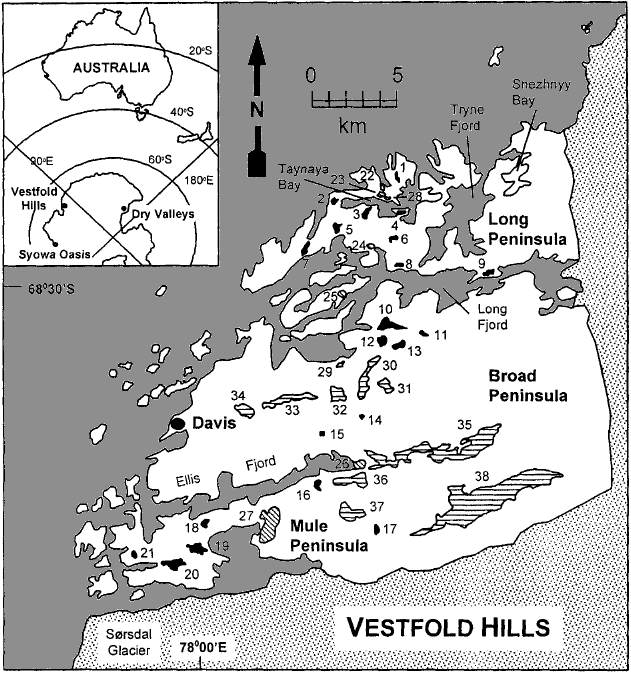
\includegraphics{intro_figures/vestfold_map.png}
\caption[Map of the Vestfold Hills]{A map of the Vestfold Hills showing fjords, bays and lakes (numbered). The Southern Ocean is shown in grey, meromictic lakes coloured in black, seasonally isolated lakes and basins are striped and the continental ice-shelf is stippled. Inset is the position of the Vestfold Hills relative to Australia and to the Antarctic coastal oases. The lakes are: (1) unnamed lake 2, (2) Organic Lake, (3) Pendant Lake, (4) Glider Lake, (5) Ace Lake, (6) unnamed lake 1, (7) Williams Lake, (8) Abraxas Lake, (9) Johnstone Lake, (10) Ekho Lake, (11) Lake Farrell, (12) Shield Lake, (13) Oval Lake, (14) Ephyra Lake, (15) Scale Lake, (16) Lake Anderson, (17) Oblong Lake, (18) Lake McCallum, (19) Clear Lake, (20) Laternula Lake and (21) South Angle Lake. Map image is from \citet{Gibson1999} with some minor modifications.}
\label{fig:vestfold_map}

\end{figure}

The region is made up of three large peninsulae, Broad, Mule and Long Peninsula, separated by fjords connected to the sea.
Some of these are large, such as Ellis Fjord, which is 10 km long, up to 100 m deep and has become a stratified system due to its restricted opening to the ocean \cite{Burke1988}.
The region was formed approximately 10,000 years ago in the early Holocene as the continental ice receded and the rocky peninsulae rose above sea-level \cite{Zwartz1998}. 

The Vestfold Hills were first sighted and named in 1935 \cite{Law1959}.
Only intermittent expeditions occurred in the area until the establishment of Davis Station (68$^{\circ}$33$'$S, 78$^{\circ}$15$'$E) in 1957 \cite{Law1959}. 
A continuous presence has been maintained since. %sometime
There Vestfold Hills region was immediately noted for its extensive ice-free land and the numerous lakes \cite{Johnstone1973}.

The Australian Antarctic Data Centre lists more than 3,000 water bodies mapped in the Vestfold Hills, ranging in area from 1 to 8,757,944 m$^2$. %check this fact.
More than 300 lakes and ponds have been described, including approximately 20\% of the world's meromictic lakes \cite{Gibson1999}. %check this fact.
These are of particular interest because the anoxic bottom waters help preserve a paleogeological record in the sediments.
This can tell us about the region and particularly climatic changes.
Stratified lakes provide a unique opportunity to describe microbial populations along chemical gradients, but within a single water body. 
%Show a map of some of the main lakes in the Vestfold Hills
%Nutrient status? (see Burton 1981) temperature? weather? major ions? (see Burton1981). recorders of climate change in the sediment and in the location of the chemocline,what occurs in each zone


\subsection{Biology of the Vestfold Hills}

The Vestfold Hills is an oasis for life.
Here is a breeding ground for seabirds, penguins and seals.
Plant life exists as mosses and lichens.
Most of the life is microbial.


%------------------------------------------------------------------------------------------

\section{Cultivation and microscopy-based Antarctic microbiology}

Microbiological studies have been conducted in the lakes regions since X.
These were conducted using cultivation and/or microscopy-based identification and quantification. 
\emph{Eucarya} were identified with microscopy based approaches.
For \emph{Bacteria}, only those that could be isolated, distinguished by morphology or biochemical tests were readily identifiable.
Were Archaea known?

\subsection{Viruses}
%Any cultured viruses?
As obligate parasites, culturing viruses is made problematic by the need to have a susceptible host in culture.
Furthermore, host specificity can be extremely narrow so any assessment of viral diversity by cultivation is highly limited.
This is compounded by the logistical constraints of conducting field work in Antarctica.

Most studies of Antarctic viruses have been confined to diversity analyses based on the electron micrographs of \ac{VLP} morphotypes or visibly infected cells. 
Electron micrographs are able to distinguish to some extent tailed bacteriophages such as myo- sipho- and podo- viruses from one another due to tail morphology.
For tailess viruses with icosohedral symmetry, morphology alone provides hardly any distinguishing features apart from capsid size.
Other metrics used to assess viruses in the environment include enumeration, virus to bacteria ratios, visibly infected cells and viral production rates.

Overall, pioneering work on viruses has made several noteworthy observations. 
\begin{enumerate}
\item Viruses are possibly more abundant in high latitude lakes than lower latitude.
\item Burst sizes of viruses are lower in high latitude lakes than in low latitude.
\item Viral abundance appears to correlate positively with salinity.
\item As food chains in Antarctic Lakes are truncated, viruses may play an increased importance in Antarctic lakes, particularly in increasing secondary production through the microbial loop.
\item %viral to bacterial ratios???
\item %viral production.
\end{enumerate}
In the absence of metazoan grazers, viruses are hypothesized to play an increased role in the microbial loop in Antarctic systems \cite{Kepner1998} and as drivers of microbial evolution \cite{Anesio2011}. 
This idea has been supported by microscopy-based observations of viral density, virus to bacteria ratios and infection rates that are different in Antarctic lakes than lower latitude systems \cite{Laybourn-Parry2001, Madan2005, Laybourn-Parry2007, Sawstrom2007}. 
Cold environments are hypothesized to be a `hotspot' of viral diversity.
However, molecular methods are required to validate this claim.

%------------------------------------------------------------------------------------------

\section{Molecular approaches used in Antarctic lake systems}
\label{in:mol}
The majority of molecular-based studies of Antarctic aquatic microbial communities have made use of \ac{PCR} amplification of \ac{SSU} sequences to survey the diversity of \emph{Bacteria}
 and in some cases \emph{Archaea} and \emph{Eucarya} \tabref{tab:pcr_lakes}.
Microbial composition has been determined by cloning and sequencing of \ac{rRNA} gene amplicons exclusively 
\cite{Bowman2000a, Bowman2000, Gordon2000, Christner2001, Purdy2003, Karr2006, Matsuzaki2006, Kurosawa2010, Bielewicz2011}, 
although most studies have also made use of \ac{DGGE} to provide a molecular ``fingerprint'' of the community 
\cite{Pearce2003a, Pearce2003b, Karr2005, Pearce2005a, Pearce2005b, Unrein2005, Glatz2006, Mikucki2007, Mosier2007, Schiaffino2009, Villaescusa2010}.
Functional genes have also been targeted using \ac{PCR} amplification to assess the potential of biochemical processes occurring, such as nitrogen fixation \cite{Olson1998}, 
ammonia oxidation \cite{Voytek1999}, anoxygenic photosynthesis \cite{Karr2003}, and dissimilatory sulfite reduction \cite{Karr2005, Mikucki2009}. %add in new studies
%\begin{landscape}

\begin{table}
\caption[PCR-based studies of Antarctic Lakes]{Studies of Antarctic Lakes that have made use of PCR amplification and sequencing of marker genes.}
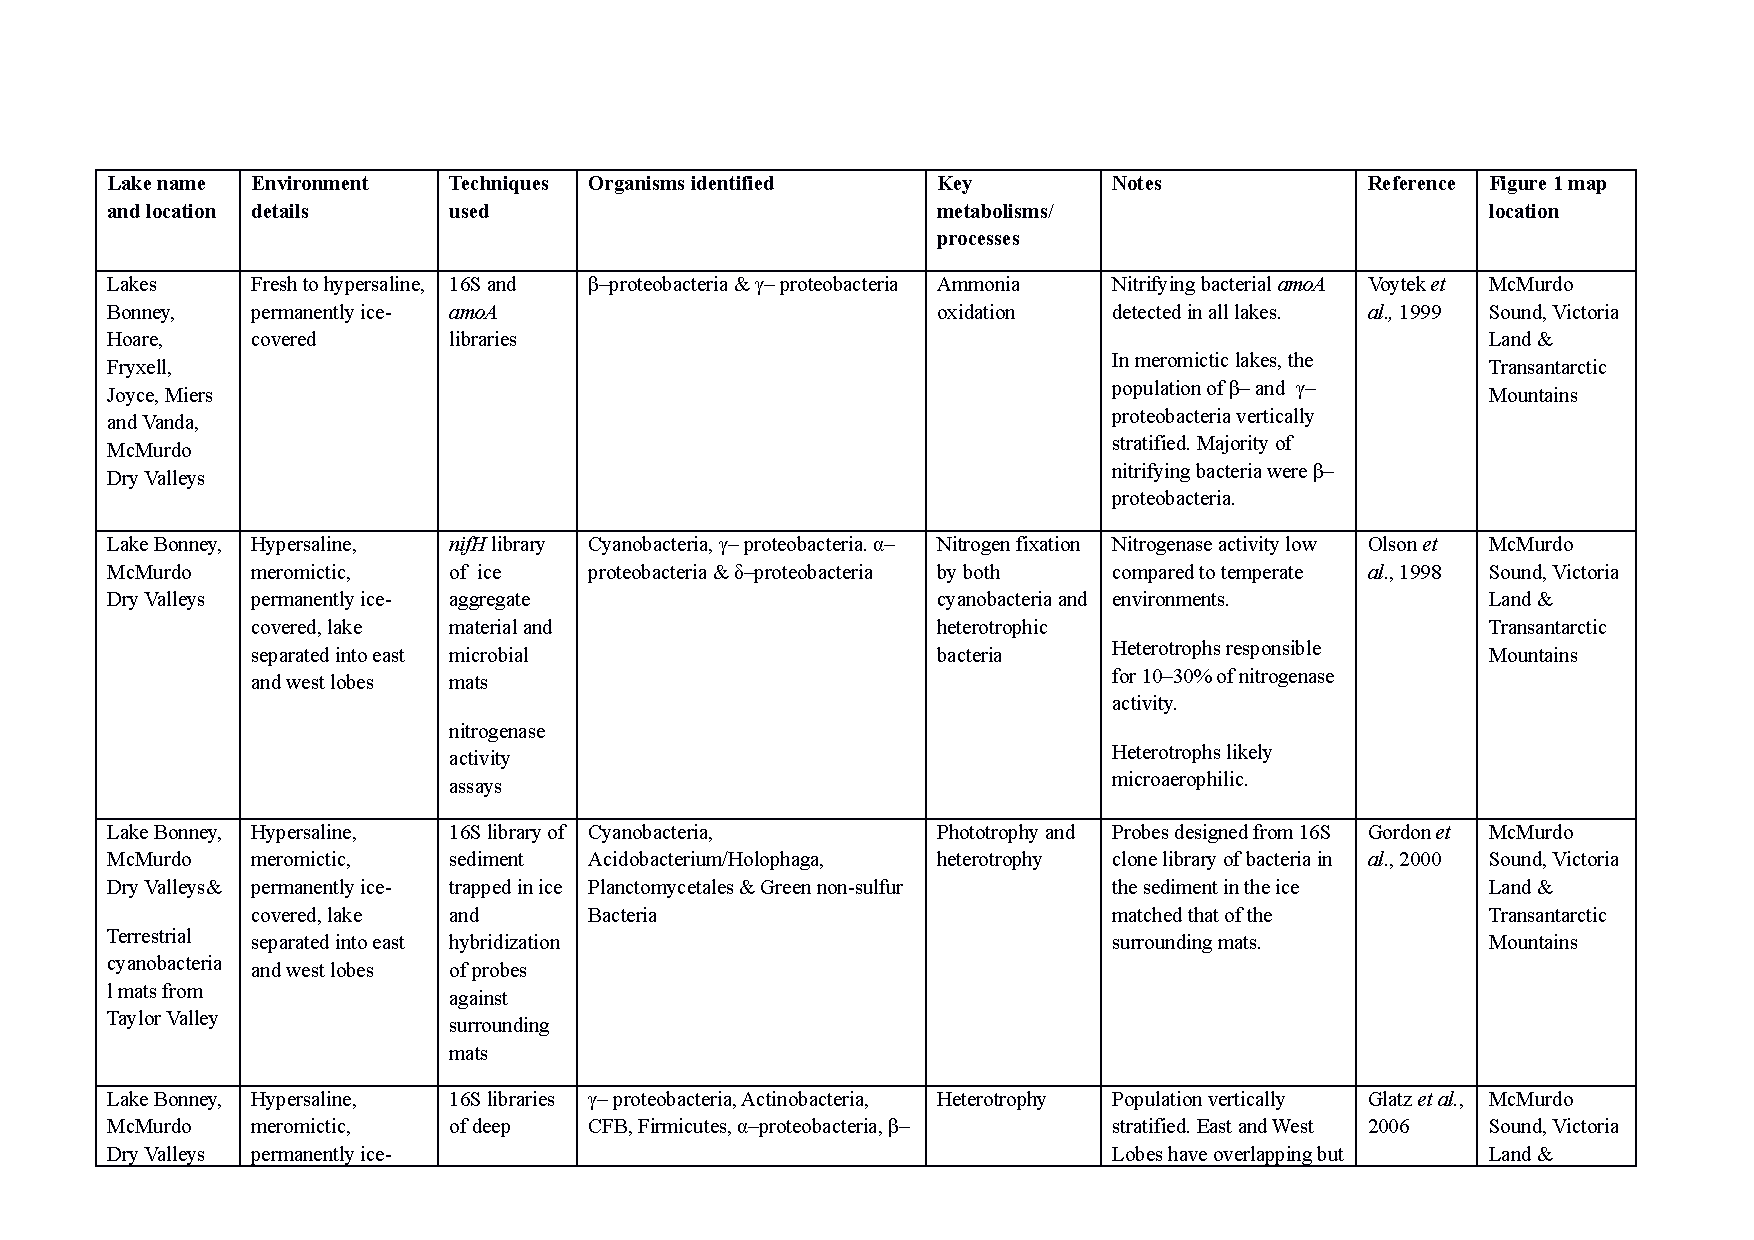
\includegraphics{intro_figures/molecular_studies_lakes.pdf}
\label{tab:pcr_lakes}
\end{table}

\end{landscape}


%-----------------------------------------------------------------------------------------

\section{Insights from Antarctic molecular studies}
\label{in:insights}
\subsection{Bacterial diversity: adaptation to unique physical and chemical conditions}
The vast majority of molecular studies of Antarctic lakes have focused on bacteria.
Consistent with the wide range of physical and chemical properties of Antarctic lakes, a large variation in species assemblages have been found.
While exchange of microorganisms must be able to occur between lakes that are in close vicinity to each other, 
the picture that has emerged from the data to date is that microbial populations are relatively unique to each type of isolated system. 
Nonetheless, certain trends in bacterial composition are also apparent.

Focusing on the similarities, lakes of equivalent salinities tend to have similar communities.
Hypersaline lakes from the Vestfold Hills \cite{Bowman2000} and McMurdo Dry Valleys \cite{Glatz2006, Mosier2007} were all dominated by \emph{Gammaproteobacteria} and members of the Bacteroidetes
 as well as harboring lower abundance populations of \emph{Alphaproteobacteria}, \emph{Actinobacteria}, and \emph{Firmicutes}.
The surface waters of saline lakes resemble marine communities dominated by \emph{Bacteroidetes}, \emph{Alphaproteobacteria} and \emph{Gammaproteobacteria},
 but divisions such as \emph{Actinobacteria} and specific clades of \emph{Cyanobacteria} have been found to be overrepresented compared to the ocean \cite{Lauro2011}.
Sediments from saline lakes in the Vestfold Hills \cite{Bowman2000a} and Nuramake-Ike in the Syowa Oasis \cite{Kurosawa2010} were very similar, 
containing in addition to the surface clades, \emph{Deltaproteobacteria}, \emph{Planctomycetes}, \emph{Spirochaetes}, \emph{Chloroflexi} (green non-sulphur bacteria), \emph{Verrucomicrobia} and representatives of candidate divisions.
Plankton from freshwater lakes were characterized by an abundance of \emph{Betaproteobacteria}, although \emph{Actinobacteria}, \emph{Bacteroidetes}, \emph{Alphaproteobacteria} and \emph{Cyanobacteria} were also prominent \cite{Pearce2003a, Pearce2005a, Pearce2005b, Schiaffino2009}. 

\subsubsection{Bacterial diversity defined by nutrients}
Differences in bacterial community structure are also influenced by nutrient availability.
In studies of freshwater lakes in the Antarctic Peninsula and the South Shetland Islands, cluster analysis of \ac{DGGE} profiles grouped together lakes of similar trophic status 
\cite{Schiaffino2009, Villaescusa2010}.
Most of the variance in community structure could be explained by related chemical parameters such as phosphate and dissolved inorganic nitrogen.
Similarly, three freshwater lakes, Moss, Sombre and Heywood on Signy Island are alike except that Heywood Lake is enriched by organic inputs from seals.

Bacterial composition in each lake changed from winter to summer and this was again correlated to variation in physico-chemical properties \cite{Pearce2005a}. 
The bacterial population of Heywood Lake had shifted from a dominance of \emph{Cyanobacteria} towards a greater abundance of \emph{Actinobacteria} and marine \emph{Alphaproteobacteria} \cite{Pearce2005b}.
This hints at a link between a copiotrophic lifestyle in the Heywood Lake \emph{Actinobacteria} and inhibition of Antarctic freshwater \emph{Cyanobacteria} by eutrophication. 
This type of study exemplifies how inferences can be made about taxa and function by examining population changes over time and over gradients of environmental parameters.

\subsubsection{Bacterial biogeography}
The relative isolation and diverse chemistries of the lakes facilitates biogeographical and biogeochemical studies. 
The anoxic and sulfidic bottom waters of some meromictic lakes form due to a density gradient that precludes mixing. 
Although sedimentation from the upper aerobic waters may occur, 
there is little opportunity for interchange of species with the bottom water of lakes allowing for greater divergence in community composition as nutrients can become depleted 
and products of metabolism can accumulate.
As a result, distinct distributions of bacterial groups can inhabit these strata, and different types of microorganisms can be found in equivalent strata in different lakes. 
A good example of this is the presence of common types of purple sulphur bacteria (\emph{Chromatiales})and \ac{GSB}(\emph{Chlorobi}) 
in some meromictic lakes and stratified fjords in the Vestfold Hills \cite{Burke1988},
compared to diverse purple non-sulphur bacteria in Lake Fryxell in Victoria Land \cite{Karr2003}. 
%Check if these aren't Roseobacters
In Lake Bonney, the east and west lobes harbor overlapping but distinct communities in the suboxic waters \cite{Glatz2006}.
The east lobe was dominated by \emph{Gammaproteobacteria} and the west lobe by \emph{Bacteroidetes}, illustrating how divergent communities can form from the same seed population. 
In contrast, ice communities are more readily dispersed by wind, aerosols and melt-water. 
16S \ac{rRNA} gene probes designed from bacteria trapped in the permanent ice-cover of Lake Bonney hybridized to microbial mat libraries sourced up to 15 km away \cite{Gordon2000}.
This demonstrates how a single lake may encompass microorganisms that are geographically dispersed, while also harboring others that have restricted niches and are under stronger selection pressure.


\subsubsection{Bacterial diversity of Lake Vostok}
Subglacial systems, such as Lake Vostok, have been isolated from the open environment for hundreds of thousands to millions of years \cite{Siegert2001}.
As a result they provide a reservoir of microorganisms that may have undergone significant evolutionary divergence from the same seed populations that were not isolated by the Antarctic ice cover. 
Lake Vostok is approximately 4 km below the continental ice-sheet making it extremely difficult to determine suitable means for accessing the lake without inadvertently contaminating it with biological
 or chemical matter \cite{Inman2005, Wingham2006, Lukin2011, Gramling2012, Jones2012}. 
To date, molecular microbial studies have concentrated on the accretion ice above the ice-water interface \cite{Priscu1999, Christner2001}.
Accretion ice has been found to contain a low density of bacterial cells from \emph{Alphaproteobacteria}, \emph{Betaproteobacteria}, \emph{Actinobacteria} and \emph{Bacteroidetes} divisions closely allied to other cold environments.
Molecular signatures of a thermophilic \emph{Hydrogenophilus} species were also identified in accretion ice 
raising the possibility that chemoautotrophic thermophiles were delivered to the accretion ice from hydrothermal areas in the lake’s bedrock \cite{Bulat2004, Lavire2007}.
However, interpretation of results from samples sourced from the Lake Vostok bore hole are very challenging as it is difficult to differentiate contaminants from native Vostok microorganisms.
From a study that assessed possible contaminants present in hydrocarbon-based drilling fluid retrieved from the Vostok ice core bore hole, 
six phylotypes were designated as new contaminants \cite{Alekhina2007}. 
Two of these were \emph{Sphingomonas} phylotypes essentially identical to those found in the accretion ice-core \cite{Christner2001},
 which raises question about whether bacterial signatures identified from the ice-cores are representative of Lake Vostok water,
 and further highlights the ongoing problem of causing forward contamination into the lake.

\subsection{\emph{Archaea}: methanogens and haloarchaea}
\emph{Archaea} have been detected mainly in anoxic sediments and bottom waters from lakes that range in salinity from fresh to hypersaline, 
and those with known isolates are affiliated with methanogens or haloarchaea \cite{Bowman2000, Bowman2000a, Purdy2003, Kurosawa2010, Lauro2011}.
%relate how this is different to marine deep waters where Crenarchaea are abundant.
Anoxia allows for the growth of methanogenic \emph{Archaea} that mineralize fermentation products such as acetate, H$_2$ and CO$_2$ into methane, thereby performing an important step in carbon cycling.
The acetoclastic methanogens thrive in environments where alternative terminal electron acceptors such as sulfate and nitrate have been depleted. 
%This may be why there are none in Organic Lake as there is still sulfate.

One example of this is Lake Heywood where methanogenic \emph{Archaea} were found to comprise 34\% of the total microbial population in the freshwater sediment, 
the majority of which were \emph{Methanosarcinales} which include acetate and C1-compound utilizing methanogens \cite{Purdy2003}. 

In general, archaeal populations appear to be adapted to their specific lake environment.
Sediments from saline lakes of the Vestfold Hills were inhabited by members of the \emph{Euryarchaeota} typically found in sediment and marine environments 
with the phylotypes differing between the lakes examined \cite{Bowman2000a}. 
While a phylotype similar to \emph{Methanosarcina} was identified, the majority were highly divergent. 
Similarly, \emph{Methanosarcina} and \emph{Methanoculleus} were detected in Lake Fryxell but other members of the \emph{Euryarchaeota} and \emph{Crenarchaeota} (a single sequence) were divergent, 
clustering only with marine clones \cite{Karr2006}. 
Based on the lake chemical gradients and the location of these novel phylotypes in the water column the authors speculated these archaea may be have alternative metabolisms such as anoxic methanotrophy or sulphur-utilization. 

In sediments from Lake Nurume-Ike in the Langhovde region, 205 archaeal clones grouped into three phylotypes, 
with the predominant archaeal clone being related to a clone from Burton Lake in the Vestfold Hills, while the other two did not match to any cultivated species \cite{Kurosawa2010}. 
In hypersaline lakes where bottom waters do not become completely anoxic, methanogens are not present and \emph{Archaea} have extremely low abundance. 
For example, only two archeael clones of the same phylotype were recovered from deep water samples from Lake Bonney \cite{Glatz2006}, 
and Organic Lake in the Vestfold Hills had an extremely low abundance of archaeal clones related to \emph{Halobacteriales} \cite{Bowman2000}. 
In contrast to these stratified hypersaline lakes, the microbial community in the extremely hypersaline Deep Lake is dominated by haloarchaea \cite{Bowman2000}. 
Many of the clones identified from Deep Lake are similar to \emph{Halorubrum} (formerly \emph{Halobacterium}) \emph{lacusprofundi} which was isolated from the lake \cite{Franzmann1988}. 

\subsection{\emph{Eucarya} perform multiple ecosystem roles}

Single-celled \emph{Eucarya} are important members of Antarctic aquatic microbial communities.
In many Antarctic systems, eucaryal algae are the main photosynthetic organisms and in others, only heterotrophic protists occupy the top trophic level. 
As eucaryal cells are generally large with characteristic morphologies, microscopic identifications have been used. 
However, microscopy is unable to classify smaller cells such as nanoflagellates with high resolution, although these may constitute a high proportion of algal biomass.
For example, five morphotypes of \emph{Chrysophyceae}, evident in Antarctic lakes were unidentifiable by light microscopy but were able to be classified using \ac{DGGE} and \textsc{DNA} sequencing \cite{Unrein2005}.
Consistent with this, molecular studies specifically targeting eucaryal diversity \cite{Unrein2005, Mosier2007, Bielewicz2011} have identified a much higher level of diversity than previously suspected,
 and the studies have discovered lineages not previously known to be present such as silicoflagellates of the family \emph{Dictyochophyceae} \cite{Unrein2005} and fungi \cite{Mosier2007, Bielewicz2011}.

Most \emph{Eucarya} in Antarctic lakes are photosynthetic microalgae that are present in marine environments with a wide distribution including chlorophytes, haptophytes, cryptophytes and bacillariophytes.
Molecular methods have afforded deeper insight into the phylogenetic diversity within these broader divisions and have revealed some patterns in their distribution. 
Using 18S \ac{rRNA} gene amplification and \ac{DGGE}, the same chrysophyte phylotypes were identified in lakes from the Antarctic Peninsula and King George Island 
despite being 220 km apart \cite{Unrein2005} indicating these species may be well-adapted to Antarctica or highly dispersed.
Similarly, an unknown stramenopile sequence was detected throughout the 18S \ac{rRNA} clone libraries of Lake Bonney 
demonstrating a previously unrecognized taxon occupied the entire photic zone in the lake \cite{Bielewicz2011}. 
In constrast, other groups showed distinct vertical and temporal distributions with cryptophytes dominating the surface, 
haptophytes the midwaters and chlorophytes the deeper layers during the summer while stramenopiles increased in the winter \cite{Bielewicz2011}. 
Further studies are necessary to determine the basis for apparent specific adaptations of some species to particular lakes or lake strata, and for the cosmopolitan distribution of others.
Here, molecular based research of the kind that has been applied to bacteria such as functional gene surveys will undoubtedly help answer these questions.
%add in new studies of photosynthetic genes

\subsection{Functional gene studies of Antarctic lakes}

\subsection{Integrative studies to derive whole ecosystem function}
%----------------------------------------------------------------------------------------------------------------------


\section{Limitations of taxonomic surveys}
\label{in:pcrlimits}

Inferring functional potential from taxonomic surveys can be problematic due to species or strain level differences in otherwise related bacteria.
For example, the majority of the \emph{Gammaproteobacteria} in hypersaline lakes were relatives of \emph{Marinobacter} suggesting that this genus is particularly adapted to hypersaline systems
\cite{Bowman2000a, Glatz2006, Matsuzaki2006, Mosier2007}.
Nonetheless, \emph{Marinobacter} species from different lakes appeared biochemically distinct
 as isolates from hypersaline lake Suribati-Ike were all able to respire \ac{DMSO} but not nitrate \cite{Matsuzaki2006}. 
In contrast, those from the west lobe of Lake Bonney were all able to respire nitrate \cite{Ward1997}. 
Interestingly, in the east lobe of the same lake, nitrate respiration was inhibited although a near-identical \emph{Marinobacter} phylotype was present; 
it was speculated that the inhibition may have been caused by an as yet unidentified chemical factor \cite{Ward2005, Glatz2006}. 

This also applies to \emph{Eucarya}, as the influence of flagellates on ecosystem function is not necessarily clear-cut as they can simultaneously inhabit several trophic levels. 
For instance, in Ace Lake the mixotrophic phytoflagellate \emph{Pyramimonas gelidocola} derives a proportion of its carbon intake through bacterivory \cite{Bell2003} 
but in the nearby Highway Lake, it uptakes dissolved organic carbon \cite{Laybourn-Parry2005}. 
This again illustrates potential limitations for deriving ecosystem level functions from taxonomic studies alone, even with taxa that appear physiologically straightforward. 

%More examples eg. limitations of functional gene surveys due to horizontal gene transfer.


%--------------------------------------------------------------------------------------------------------------------

\section{`-omics' approaches}
Metagenomic studies have assessed both the taxonomic composition and genetic potential of lake communities, and in some cases have linked function to specific members of the community 
\cite{Lopez-Bueno2009, Ng2010a, Lauro2011, Yau2011, Varin2012}.
When coupled with functional ``omic'' techniques (to date metaproteomics has been applied, but not metatranscriptomics or stable isotope probing), 
information has also been gained about the genetic complement that has been expressed by the resident populations \cite{Ng2010a,Lauro2011}.
More detailled description of the advances of `-omics' approaches is detailed in the introduction of chapter 2.
%Refer forward.

Metagenomics has enabled unprecedented insight into viral diversity and ecology by permitting more precise classification, information on genetic content and discovery of novel species. 
Metagenomic analysis of the viriome of the freshwater Lake Limnopolar, Livingston Island uncovered the greatest depth of viral diversity of any aquatic system to date \cite{Lopez-Bueno2009}.
Representatives from 12 viral families were detected, but unlike the two previous viromes that had been published at that time using comparable techniques, ss\textsc{DNA} viruses and large ds\textsc{DNA} viruses that putatively infect eucarya were the dominant viral types rather than bacteriophages. 
The ss\textsc{DNA} viruses were related to circoviruses, geminiviruses, nanoviruses and satellites; viruses previously only known to infect plants and animals indicating they are much more diverse than previously suspected and may constitute new viral families. 
Samples taken in summer showed a shift in the viral community composition towards phycodnaviruses similar to Ostreococcustauri virus, OtV5. 
This shift potentially reflects an increase in the host algae that are stimulated to bloom by the increased light availability.

Understanding of Antarctic viral diversity and ecology is still in its early days as a complete viral survey is problematic due to the lack of a universal viral gene or even universal genetic material. 
Furthermore, the enormous depth of viral diversity remains largely unsampled so most viral sequences have no significant similarity to sequence data repositories \cite{Lopez-Bueno2009}. 
What is clear is that viruses perform a crucial role in shaping community structure, driving host evolution, contributing to the dissolved nutrient pool, and understanding them is essential to understanding ecosystem function \cite{Danavoro2011}. 
%-----------------------------------------------------------------------------------------------------------------

\section{Objectives}
This study aimed to use a primarily metagenomic approach complemented with microscopy and metaproteomics to gain an integrative understanding of whole ecosystems.
Ace Lake and Organic Lake were chosen as the study sites because as meromictic systems, differences in the microbial population can be examined across vertical gradients, they are also largely isolated, as marine-derived systems, adaptation of marine microbiota to lake system can be examined, they are sites of moderate diversity and may be reservoirs of unknown taxa.
Using this methodology, not only can the taxonomic composition of the lakes be determined but also the functional potential of the microbial population and insight into the active members of the community.
The objectives of the research were:

\begin{enumerate}
\item 
  To develop complementary analyses to metagenomic analysis.

\item
  To determine the microbial and viral composition of the lake communities and their functional potential.

\item
  To identify the genes expressed by the community.

\item
  To reconstruct genomic information of dominant taxa of interest.

\item
  To integrate environmental and biological data to model the lake microbial interactions and geochemical processes.

\end{enumerate}

\chapter[Application of metaproteomics to complementary to Ace Lake metagenomic analysis]{Application of metaproteomics to complement Ace Lake metagenomic analysis}
\label{ch:ace}
\acresetall

%-----------------------------------------------------------------------------------------------
\section*{Co-authorship statement}
\addcontentsline{toc}{section}{Co-authorship statement}

Sections from this chapter~\ref{ch:ace} have been published as:\\

Federico M. Lauro, Matthew Z. DeMaere, \textbf{Sheree Yau}, Mark V. Brown, Charmaine Ng,
David Wilkins, Mark J. Raftery, John A.E. Gibson, Cynthia Andrews-Pfannkoch, Matthew Lewis,
Jeffery M. Hoffman,Torsten Thomas, and Ricardo Cavicchioli. 
An integrative study of a meromictic lake ecosystem in Antarctica.\\
\emph{\underline{The ISME Journal}} \\
5:879--895, 2011.\\

I performed the metaproteomic mass spectra analysis, epifluorescence imaging,
microbial and viral counts and wrote the corresponding sections of the publication.
Only these parts of the publication are included in the results and discussion of this chapter.

Analyses performed by others that support the work presented in this chapter are as follows:
Research was designed by Federico Lauro, Mark Brown, Torsten Thomas, John Gibson and Ricardo Cavicchioli.
Sample collection was performed by Federico Lauro, Mark Brown, Torsten Thomas, Jeffery Hoffman and Ricardo Cavicchioli.
\textsc{DNA} extraction and clone library preparation of 2006 samples was performed by Cynthia Andrews-Pfannkoch and Jeffery Hoffman of the \ac{JCVI}.
\textsc{DNA} sequencing quality control was performed by Matthew Lewis of the \ac{JCVI}.
Metagenomic sequence filtering, mosaic assembly and annotation was performed by Matthew DeMaere.
Protein extraction, one-dimensional sodium dodecyl sulphate-polyacrylamide gel electrophoresis and liquid chromatography mass spectrometry performed by Charmaine Ng.
Assistance in mass spectra analysis was provided by Mark Raftery.
\newpage

%----------------------------------------------------------------------------------------------
\section{Abstract}
Ace Lake is a saline meromictic lake in the Vestfold Hills, Antarctica.
As a system of moderate biological complexity with extensive historic physical and chemical data, it was chosen as a site to implement an integrative study of the whole lake ecosystem.
Metagenomic analysis of Ace Lake revealed a strong separation of the microbial taxa and metabolic genes according to the lake's water column structure.
The aerobic mixolimnion resembles a marine surface water microbial community with dominant members of the SAR11 clade, \emph{Synechococcus}-like \emph{Cyanobacteria}, \emph{Flavobacteria} and \emph{Actinobacteria}.
At the oxic--anoxic interface resides a near-clonal population of \ac{GSB} termed C-ace while the anoxic monimolimnion contains an extremely diverse assemblage that includes methanogenic \emph{Archaea}, \ac{SRB} and diverse candidate divisions.
The viral population comprises abundant bacteriophages as well as large phycodnaviruses.
From the functional marker genes, the nutrient cycling capacity of the community was inferred.
Metaproteomic analysis of the \ac{GSB} layer using the matched metagenomic information allowed detailled description of the metabolism of the \ac{GSB}.
This study aimed to validate metagenomic inferences of the whole lake ecology and gain new insights into the expressed protein complement of the Ace Lake community.
Preliminary metaproteomic analysis using cross-species matching of mass spectra to the \ac{NR} database had already shown few identifications.
This was significantly improved by using assembled metagenomic sequence as the protein search database.



%---------------------------------------------------------------------------------------------
\section{Introduction}
Ace Lake is a meromictic saline lake in the Vestfold Hills, Antarctica. 
It is possible the most intensively studied of all the meromictic lakes in the Vestfold Hills.
Extensive physical, chemical and biological data has been collected from Ace Lake in the last decades \cite{Rankin1999}.
%This is summarised in the figure of the whole lake. %figure of lake.
An analysis of the 16S \ac{SSU} diversity was completed of the sediment showed microbial diversity was reduced \cite{Bowman2000a}.
%What else? about the diversity from Bowman paper? Link to the intro.

Ace Lake is a highly stratified lake system, 25 m deep at its deepest point.
It is ice-covered for approximately 9 months of the year and thaws some summers. %check
Water is marine-derived and a largely neutral water balance has ensured salinity is close to that of seawater.
Although a lens of fresher water from melted surface ice can be generated in the summer months, this only mixes when the lake is ice-free and not to great depth \cite{Rankin1999}.
The lake is physically separated into an aerobic mixolimnion, a steep chemocline/oxycline at 12.7 m and an anoxic monimolimnion below.
The monimolimnion is sulfidic and methanogenic; both compounds have presumably accumulated through activity from \ac{SRB} and methanogenic archaea respectively.

As a physically and chemically well-characterised system of moderate diversity, Ace Lake was chosen as a model ecosystem to implement an integrated metagenomic and metaproteomic analysis.
Combining both approaches would allow assessment of the metabolic potential of the system and identify the active members of the community and processes at time of sampling.
Samples were obtained down the depth profile at 5, 11.5, 12.7, 18 and 23 m depths corresponding to each of the three zones.
Sampling was conducted as part of the \ac{GOS} expedition \cite{Rusch2007} by using size fractionation of microbial biomass onto 3.0, 0.8 and 0.1 \textmu{}m membrane filters.
%consider leaving above line out.

Microbial and viral community composition was assessed from the metagenomic dataset.
Significant differences were found in taxonomic composition of each size fraction within each sample depth and stratification of the microbial community between the three zones of Ace Lake.
The mixolimnion community is similar to a marine surface water assemblage consisting of a high abundance of the SAR11 clade of \emph{Alphaproteobacteria} related to ``\emph{Candidatus} Pelagibacter ubique'' and green algae of the order \emph{Mamiellales}.
However, diversity is reduced by one order of magnitude reduced \cite{Lauro2011}.
Unlike Southern Ocean surface water, the mixolimnion is overrepresented in \emph{Cyanobacteria} related to \emph{Synechococcus} and \emph{Actinobacteria}, which may represent taxa that mark the transition of a marine to lake community.
A dense, near clonal population of \acl{GSB} related to \emph{Chlorobium} termed C-ace reside at the chemo/oxycline at 12.7 m \cite{Ng2010a, Lauro2011}.
Below, in the anoxic monimolimnion is a diverse, primarily heterotrophic community with abundant \ac{SRB} and methanogenic \emph{Archaea}.

The viral community comprising Phycodnaviridae, Myoviridae, Siphoviridae, Podoviridae and unidentified viral families \cite{Lauro2011}. 
Bacteriophage were abundant in the bottom waters, whereas the surface community, was dominated by phycodnaviruses \cite{Lauro2011}. 
Most notably, no viral signatures were found at 12.7 m depth, which is a zone occupied by a near-clonal population of \ac{GSB}. 
Mathematical modeling predicted that the absence of phage predation in the GSB could be due to an adaptation to longer cycles of growth and inactivity in response to the polar light regime. Phototrophs with faster growth rates, such as eucaryal algae and Cyanobacteria in the surface water, were predicted to be more susceptible to viral predation. 
The viral susceptibility of these phototrophs was predicted to lead to increased host genetic variation, and this was borne out in the analysis of the metagenome data \cite{Lauro2011}. 
%How abundant were the methanogens??

Preliminary metaproteomic analysis down the vertical profile of Ace Lake has been performed using a cross species genomic database comprising the \ac{NCBI} \ac{NR} database to perform protein identifications \cite{Ng2010b}.
A focused metaproteogeonomic analysis conducted on the dense \ac{GSB} layer using the matched metagenome as the database resulted in many more protein identifications compared to using the \ac{NR} database \cite{Ng2010b}.
%Put in a table of the rates of matches...
This indicates large gains in metaproteome coverage are possible using a matched metagenomic database \cite{Ng2010b}.
Significantly, \ac{GSB} appeared to be crucial in the lake ecosystem as they had the greatest genetic potential for nitrogen and carbon fixation as well as sulphur cycling\cite{Ng2010b, Lauro2011}.
Metaproteomic analysis was able to identify which proteins were actively expressed and thus the active pathways of the \ac{GSB} metabolism which are so crucial to the function of the lake \cite{Ng2010a}.

This study aimed to expand on the metagenomic analysis of the water column of Ace Lake using complementary analyses.
Metaproteomic analysis was used to identify expressed proteins of the 0.1 \textmu{}m size fraction Ace Lake using a matched metagenomic databases for protein identification to infer which taxa and metabolic processes were active at time of sampling.
To determine cellular and viral densities and validate the efficacy of size-fractionation with a modified epifluorescence microscopy procedure was developed and implemented.

A whole systems level approach was employed to piece together ecosystem functioning of a moderately complex lake system (Ng et al., 2010; Lauro et al., 2011). Ace Lake is a marine-derived meromictic saline lake in the Vestfold Hills that was isolated from the ocean ~5,000 ya. Utilizing both metagenomics and metaproteomics, a taxonomic profile of all three domains of life and viruses throughout the water column was determined as well as carbon, nitrogen and sulfur cycles. The upper oxic waters resemble a simplified marine planktonic community, below which a dense layer of GSB reside at the oxycline, while the anoxic bottom waters host a diverse assemblage of anaerobic bacteria and archaea. By adopting a whole ecosystem perspective, it was apparent that community structure and resource partitioning defined nutrient cycling. For example, a strictly-interdependent sulfur cycle was found to exist between the GSB and sulfate-reducing bacteria at the oxycline. The GSB were able to convert sulfide to sulfate but lacked assimilatory sulfate reduction capability (Ng et al., 2010; Lauro et al., 2011). It was also apparent that short circuiting of the nitrogen cycle was occurring. Nitrogen fixation proteins were not found in the metaproteome, likely due to preferential assimilation of ammonia (Ng et al., 2010; Lauro et al., 2011). Genes involved in nitrification and denitrification were underrepresented indicating the system had shifted away from nitrogen mineralization consistent with a mechanism to conserve bioavailable nitrogen (Lauro et al., 2011). It is noteworthy that these findings are in contrast to lakes in the Dry Valleys where ammonia monooxygenase genes were present in the aerobic zone of six lakes of various salinities and extents of stratification (Voytek et al., 1999).
The Ace Lake study also identified the importance of the loss of pathways including nitrification,the expansion of gene families (such as transposons) and the selection of key species (in particular GSB) as important steps in transiting the microbial population from marine to a meromictic lake ecosystem (Lauro et al., 2011). To attempt to describe and predict the effects of ecosystem change on the lake, a mathematical model was developed that described the impact of fluctuations in environmental parameters on key microbial populations in the lake. One outcome of the model was the prediction that invasion (e.g. by introduction) by GSB-infecting phage would eliminate the population and leave the lake in an unstable condition, in terms of microbial processes, and unable to recover for many years into the future (Lauro et al., 2011).

%---------------------------------------------------------------------------------------------

\section{Materials and methods}
\label{sec:ace_mm}
\subsection{Ace Lake samples}
Water samples were collected from Ace Lake (68$^{\circ}$28$'$23.2$''$S, 78$^{\circ}$11$'$20.8$''$E), Vestfold Hills, Antarctica on 21 and 22 December 2006. 
A 2 m hole positioned above the deepest point (25 m depth) of the lake was drilled through the ice cover of Ace Lake to reach the lake surface.
A volume of 1--10 L was collected by sequential size fractionation through a 20 \textmu{}m pre-filter directly onto filters 3.0, 0.8 and 0.1 \textmu{}m pore-sized, 293 mm polyethersulfone membrane filters (Rusch et al., 2007), along the depth profile as described previously \cite{Ng2010a}.
Samples were taken in the order, 23, 18, 14, 12.7, 5 and finally, 11.5 m.

After samples from each depth were collected, the sample racks were sequentially washed with 2 $\times$ 25 L 0.1 N NaOH, 2 $\times$ 25 L 0.053\% NaOCl, and 2 $\times$ 25 L fresh water. 
The sample hose was flushed with water from each depth before being applied to the filters. 
A \emph{Chlorobium} signature was identified at 5 m, but not immediately above the \ac{GSB} layer at 11.5 m. 
As the next sample taken after sampling at 12.7 m was at 5 m, and then 11.5 m, despite all equipment being thoroughly washed with bleach, NaOH and water, 
the simplest explanation for the \ac{GSB} signature at 5 m is carry-over from sampling of the dense biomass at 12.7 m. 

A sonde probe (\textsc{YSI} model 6600, \textsc{YSI} Inc., Yellow Springs, \textsc{OH}, \textsc{USA}) was used to record depth, dissolved oxygen content, pH, salinity, temperature and turbidity throughout the water column of the lake. 
Total organic carbon was determined using a total organic carbon analyzer, TOC-5000A (Shimadzu, Kyoto, Japan) equipped with a \textsc{ASI}-5000A auto sampler (Shimadzu), and particulate organic carbon by standard protocols 
\url{(http://www.epa.gov/glnpo/lmmb/methods/about.html)} 
at the Centre for Water and Waste Technology, \textsc{UNSW}.

\subsection{\textsc{DNA} sequencing and data cleanup}
\textsc{DNA} extraction and Sanger sequencing was performed on 3730xl capillary sequencers (Applied Biosystems, Carlsbad, \textsc{CA}, \textsc{USA}) and pyrosequencing on \textsc{GS20 FLX} Titanium (Roche, Branford, \textsc{CT}, \textsc{USA}) at the \acl{JCVI} in Rockville, \textsc{MD}, \textsc{USA} \cite{Rusch2007}. 
The scaffolds and annotations will be available via \ac{CAMERA} and public sequence repositories such as the \ac{NCBI} and the reads will be available via the \ac{NCBI} Trace Archive. 

Sanger reads were trimmed according to quality clear ranges.
The quality of pyrosequencing reads was assessed as follows: 
a \ac{BLAST} nucleotide database was created from the Sanger reads of the 0.1 \textmu{}m fraction of samples GS230, GS231 and GS232 (see Table of metagenomic data). %%Add link to table of metagenomic data. Change sample IDs to depths?
After blasting the corresponding pyrosequencing reads against each database with a minimum bitscore of 80 and maximum e-value of 0.1, reads were binned according to length.
The percentage of reads for each bin lacking a match to the Sanger read database was recorded. 
The percentage reads at least 25\% repetitive after \textsc{MDUST} \cite{Morgulis2006} analysis at default settings, and the percentage of reads containing N's, were assessed. 
In contrast to earlier pyrosequencers \cite{Huse2007}, no length-dependent bias in reads containing N's was observed. 
However, short reads had a disproportionately high number of repeats. 
Moreover, based on the proportion of reads with no match to the Sanger data set, both very short and very long reads had a disproportionately high number of errors; an observation that was previously reported \cite{Huse2007}.

On the basis of this analysis, a three step filtering process was applied to each sample. 
Reads were initially run through the Celera \textsc{sffToCA} \cite{Miller2008} pre-processor followed by \textsc{Lucy} \cite{Chou2001} and finally, excluding the bottom 8\% and top 3\% of reads determined from the read length distribution. 
As the \textsc{sffToCA} (v5.3) pre-processor removes all reads with a perfect prefix of any other read it overcomes the `perfect duplicates’ problem \cite{Gomez-Alvarez2009}.
 
After this process, $<$5\% of the reads belonged to clusters of duplicates with three or more reads, and \ac{COG} of proteins classification of these reads showed an over-representation of category L (replication, recombination and repair) that includes mobile genetic elements, which are often duplicated, suggesting a potential biological significance for the duplicated reads. 
It is possible these residual duplications are a result of high gene copy number or localized fragility of DNA sequences that might be biasing the shear points.

\subsection{Metagenomic DNA assembly and annotation}
Mosaic assemblies were generated for each sample fraction using Celera \ac{WGS} Assembler v5.3 \cite{Myers2000}. 
For each assembly, the runtime parameters used were as outlined for 454 sequencing data in the published standard operating procedure\\ 
\url{(http://sourceforge.net/apps/mediawiki/wgs-assembler/index.php?title 1⁄4SFF\_SOP)}. 
As none of the samples can be considered clonal, these are regarded as stringent assemblies \cite{Rusch2007}. 
Each 0.1 \textmu{}m fraction assembly was a hybrid of Sanger and 454 read data, wherein the estimated genome size was manually set to minimize the number of unitigs from abundant organisms being falsely classified as degenerate \cite{Rusch2007}. 
Annotation of each sample fraction assembly was carried out using an in-house pipeline, wherein the pipeline stages consisted of genomic feature detection and subsequent annotation. 
Detected features consisted of \acp{ORF}, transfer \textsc{RNA} and \ac{rRNA}. 
Each detected \ac{ORF} was further annotated by \ac{BLAST} comparison against \ac{NR}, Swissprot and \ac{KEGG}-peptide sequence databases and by \ac{HMMER} comparison against \ac{TIGRFAM} \cite{Haft2001}, \ac{COG} \cite{Tatusov1997, Tatusov2003} and known marker genes \cite{vonMering2007}.
In all cases the cut-off e-value was a maximum of 1e$-$5. 


\subsection{Epifluorescence microscopy}
Samples of unfiltered lake water and the flow-through from 3.0 and 0.8 \textmu{}m filters from all depths were collected on November 2008 and fixed on site in formalin 1\% (v/v). 
The samples were stored at $-$80$^{\circ}$C for subsequent direct counts of cells and \acp{VLP}. 
Enumeration was performed according to the method of \citet{Patel2007} with modifications. 
%desribe the set up of the filter apparatus!
Lake water samples were filtered onto 0.01 \textmu{}m pore-size polycarbonate filters (25 mm Poretics, \textsc{GE} Osmonics, Minnetonka, \textsc{MN}, \textsc{USA}). 
Filters were air dried, then placed with the back of the filter on top of a 30 ml aliquot of 0.1\% (w/v) molten low-gelling-point agarose and allowed to dry at 30$^{\circ}$C. 
Samples were stained by the addition of 1 ml working solution (1 in 400 dilution in 0.02 \textmu{}m filtered sterile Milli-Q) of \textsc{SYBR} Gold$^{\textregistered}$ (Molecular Probes, Eugene, \textsc{OR}, \textsc{USA}) to 25 ml of mounting medium (\textsc{VECTASHIELD} HardSet, Vector Laboratories, Burlingame, \textsc{CA}, \textsc{USA}). 
Stained samples were counted immediately, or stored at $-$20$^{\circ}$C for up to a week before counting. 
Samples were visualised under wide-blue filter set (excitation 460--495 nm, emission 510--550 nm) with an epifluorescence microscope (Olympus BX61, Hamburg, Germany).


\subsection{Metaproteomic analysis}
Proteins were extracted from membrane filters from all 0.1 \textmu{}m fractions from the six depths (5, 11.5, 12.7, 14, 18 and 23 m), and \ac{1D-SDS PAGE} and in gel trypsin digestion, liquid chromatography and mass \ac{MS}, and \ac{MS-MS} data analysis and validation of protein identifications performed as previously described \cite{Ng2010a}, with minor modifications.
The specta generated were searched against the protein sequence database corresponding to that depth constructed from the 0.1 \textmu{}m mosaic assemblies. 
The number of protein sequences in each database were as follows: 5 m, 138,208; 11.5 m, 133,948; 12.7 m, 27,142; 14 m, 62,436; 18 m, 71,512; and 23 m, 128,878. 
Scaffold (version Scaffold\_2\_05\_01, Proteome Software Inc., Portland, \textsc{OR}, \textsc{USA}) was used to validate \ac{MS-MS}-based peptide and protein identifications. 
Peptide and protein identifications were accepted if they could be established at $>$95\% and 99\% probability, respectively, as specified by the Peptide Prophet algorithm \cite{Keller2002}. 
Protein identifications required the identification of at least two peptides.
 
Proteins that contained similar peptides and could not be differentiated based on \ac{MS-MS} analysis alone were grouped to satisfy the principles of parsimony and are referred to as a protein group. 
Spectral counting was used to semi-quantitively estimate protein abundance. 
The total assigned spectra that matched to each identified protein were exported from \textsc{Scaffold} 2.0. 
For similar proteins that have shared peptides (a protein ambiguity group), spectra were assigned to the protein with the most unique spectra. 
To normalise for variation in total spectra acquired between sample replicates, the number of spectra of each protein was multiplied by the average total spectra divided by the total spectra of the individual replicate. 
The spectral count of each protein was averaged across the replicates. 
As longer proteins are more likely to be detected, the average spectral counts were divided by the length of the protein. 
This value is equivalent to the normalised spectral abundance factor \cite{Florens2006, Zybailov2006}. 
In order to compare the relative abundance of proteins between depths, the normalised spectral abundance factor was divided by the average read depth of the contig (scaffold or degenerate) to which the protein mapped. 

If $>$90\% of a scaffold’s length consisted of surrogate (highly degenerate unitig) sequence, the average read depth of the surrogate was used. 
For identified proteins that were part of a protein group the longest protein length and largest read depth value in the group was used. 
Pairwise comparisons of each zone were conducted on \ac{COG} assigned proteins. 
The normalised spectral counts from each protein was aggregated based on their \ac{COG} annotation. 
All proteins that were part of an ambiguity group were confirmed to share the same \ac{COG} annotation to ensure counts were not biased because of the common spectra.

The summed spectral counts from 5 and 11.5 m (mixolimnion), and 14, 18 and 23 m (monimolimnion) were pooled. 
Statistical significance of differences between each zone was assessed using Fisher's exact test, with confidence intervals at 99\% significance calculated by the Newcombe–Wilson method and Holm-Bonferroni correction (P-value cutoff of 1e$-$5) in \ac{STAMP} \cite{Parks2010}. 
All proteins identified, including their gene identifier, normalised spectral abundance, \ac{COG} and \ac{KEGG} Orthology identifiers, \ac{KEGG} locus tag and matching \ac{COG} or \ac{KEGG} description are provided in Supplementary Table S1.



%---------------------------------------------------------------------------------------------

\section{Results and discussion}

\subsection[Epifluorescence microscopy methodology]{Development of epifluorescence microscopy methodology for cell and \acp{VLP} enumeration}
As part of the integrative study of Ace Lake, an epifluorescence microscopy methodology was developed.
Motivation for visualising microbiota from size fractionated water samples was twofold. 
Firstly, visualising microbiota from water samples allows examination of cellular morphologies and more importantly, enumeration of cells and \acp{VLP}.
Absolute cellular and \ac{VLP} densities are not easily inferred from the metagenomic data and necessitates a complementary method of determination.
Determining viral densities is extremely important as the first studies to do so found that viruses are the most numerous biological entities on the planet and likely play a large role in plankton mortality in the ocean \cite{Bergh1989,Proctor1990}. %Why is determining cellular densities important
\ac{VLP} counts from marine environments vary with depth and trophic status ranging from 10$^6$ to 10$^8$ \acs{VLP} ml$^{-1}$ \cite{Suttle2005}. %cite Fuhrman review paper too.
Viral counts from various aquatic environments have differed from site to site indicating a variable role of virally mediated mortality. %ref microbial ecology of the oceans.%cite Fuhrman review.

Secondly, size fractionation of suspended microbial biomass from aquatic environments has been utilised as part of the landmark Sargasso Sea metagenomic study \cite{Venter2004} and subsequent \ac{GOS} expedition \cite{Rusch2007}.
The Ace Lake samples were collected using the same sampling strategy as the \ac{GOS} dataset but has sequence information from all three filter sizes. 
Thus, the visualisation of microbial morphologies from each stage of the filtration process would allow validation of the filtration process.

Developing a revised method for the simultaneous counts of cells and \acp{VLP} was necessary due to inability to source 25 mm diameter 0.02 \textmu{}m pore-size Anodisc filters (Whatman) that have been long used with fluorescent nucleic acid dyes for this purpose \cite{Hennes1995, Noble1998}. 
They were marked for discontinuation in December 2008 after the take over of Whatman by \textsc{GE} Healthcare and was the cause of a global shortage that was strongly opposed by the viral ecology community \cite{Torrice2009}.
Since conducting this research, production of 25 mm Anodisc filters has resumed after the petitioning of \textsc{GE} Healthcare by the environmental virology community. 
Cost of Anodiscs filters are relatively higher than they were previously. %%%Check!
Nonetheless, the need for alternative methodolodies during the shortage was so great that alternative protocols were developed independently in other research groups \cite{Budinoff2011, Diemer2012} stressing the importance of an affordable method of direct viral counts and the utility of alternative methodologies. %Look up that poster with beads direct on slide.

Clear \ac{PCTE} filters were selected for use as a viable alternative product for the following reasons. 
\begin{enumerate}
\item They have defined pore-size. %Look up track etch technology
\item They are available in 0.015 \textmu{}m pore-size allowing capture of \acp{VLP}.
\item They have previously been used for \acp{VLP} enumeration \cite{Hara1991, Proctor1992}.
\item They have a long history of use with cellular enumeration \cite{Hobbie1977} and can therefore be easily adopted for widespread use.
\end{enumerate}

%get refs for hara1991 and Proctor1992.

There are several disadvantages to using \ac{PCTE} membranes over Anodiscs which are as follows.
\begin{enumerate}
\item Polycarbonate is not as robust as 25 mm diameter Anodisc filters that have a built in plastic support ring around the edge.
\item The polycarbonate of \ac{PCTE} filters cannot be blotted dry as the Al$_{2}$O$_{e}$ of Anodisc filters.
\item \ac{PCTE} filters appear to have high background fluorescence. %ref
\item \ac{PCTE} filters have a much slower flow rate that Anodisc filters. %ref.
\end{enumerate}

The protocol used is detailled in the materials and methods \ref{sec:ace_mm}.
The main disadvantages of using \ac{PCTE} were overcome for the purposes required for this study.
To counteract the fragility of the \ac{PCTE} filters, vacuum filtration was not performed above X pressure limit and filters.
No cracks or tears were observed during visualisation.
\ac{PCTE} filters also have a tendency to crinkle when mounted on the glass slide making visualisation of cells and \acp{VLP} on a single focal plane difficult.
Agarose was used to embed the filters to help flatten the membrane and aid in mounting.
However, this was not strictly necessary if filters were dried well and the membrane mounted carefully so that it was pressed flat against the glass slide.
The back ground fluorescence of the clear filters was low when stain is only incorporated into the mountant after filtration rather than staining in the column before filtration.

Filtration onto very small pore-size also necessitated a very strong seal of the filter column against the glass, but the slow flow-rate was not a property of the \ac{PCTE} filters that could be overcome.
As the filtration and visualisation was performed on fixed samples in the laboratory rather than in the field, the time taken for filtration of 2--3 hours for each sample, this was not deemed problematic for this study.


Overall, a viable alternative methodology was successfully developed for visualisation and enumeration of cells and \acp{VLP} using \ac{PCTE} membrane filters was successful and could be used as an alternative to Anodisc-filters \figref{fig:ace_microscopy}.
\begin{figure}
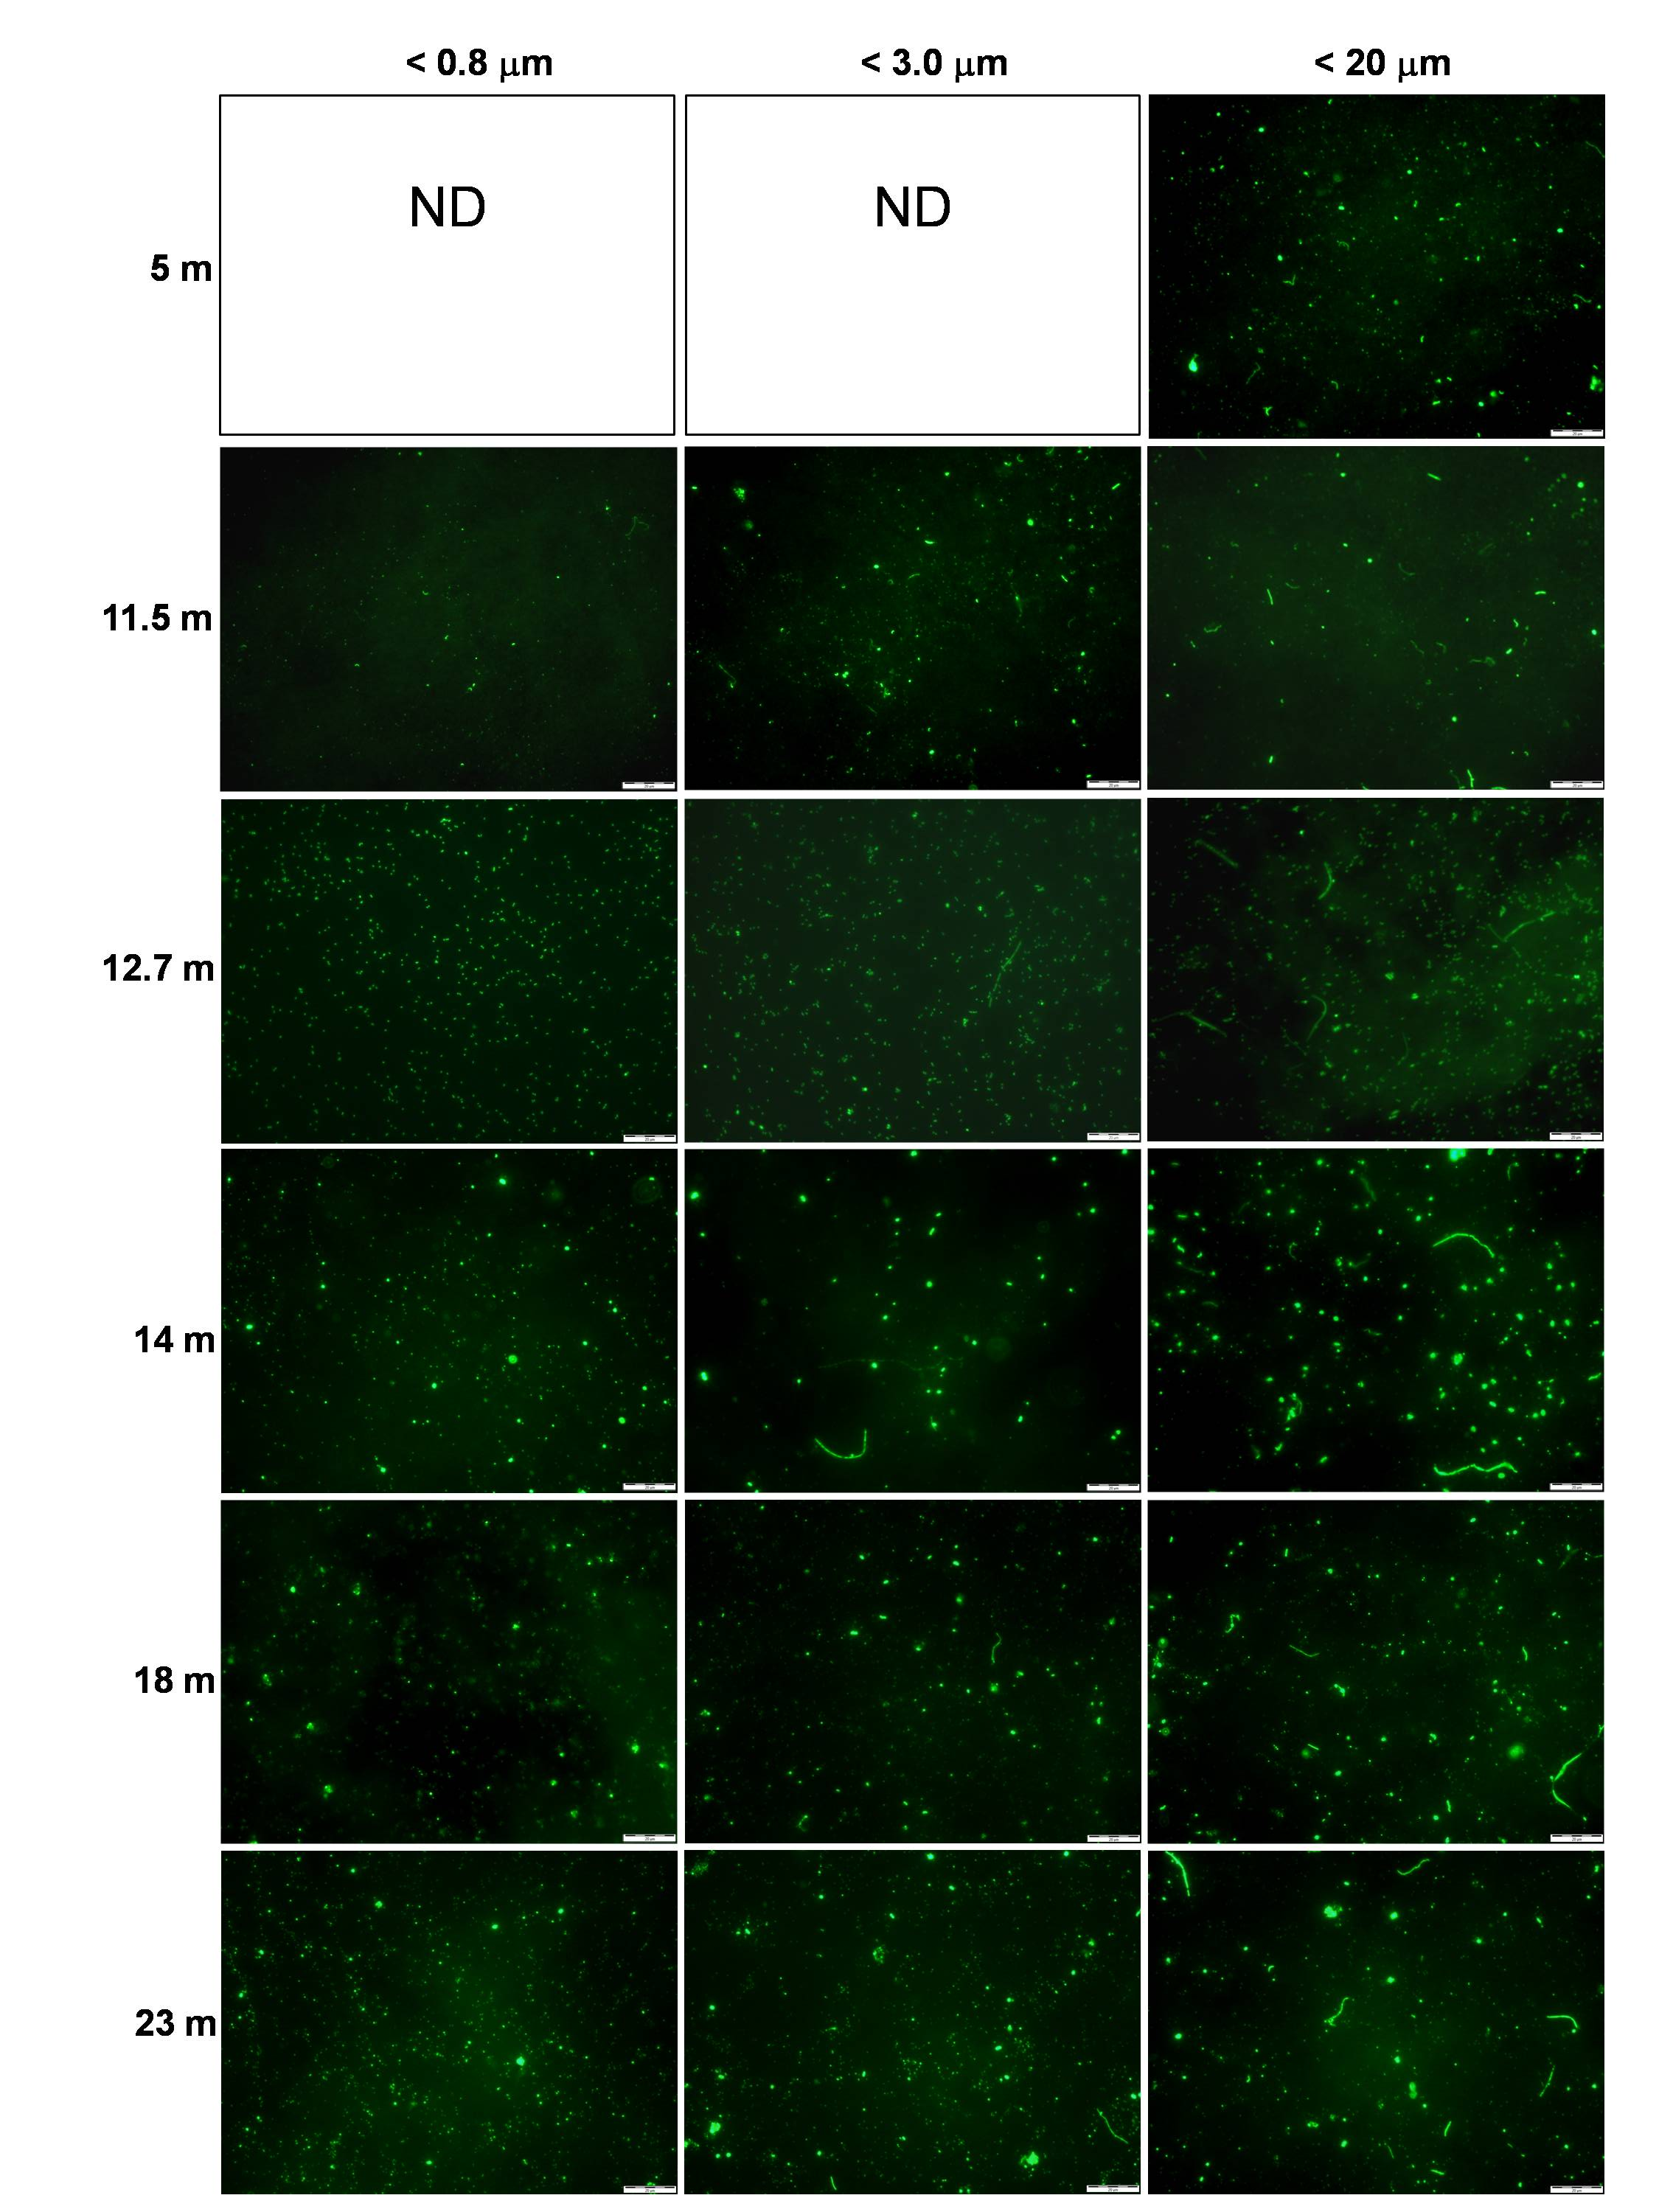
\includegraphics[width=\textwidth]{ace_figures/ace_microscopy.jpg}
\caption[Epifluorescence microscopy of Ace Lake microbiota]{Epifluorescence microscopy images of Ace Lake microbiota. Scale bar $=$ 20 \textmu{}m. ND, not determined.
}
\label{fig:ace_microscopy}

\end{figure}

To be competitive alternative to Anodisc filters in terms of accuracy of counts, a comparison of this methodolody and Anodisc-based protocols using viral samples of known densities needs to be performed.

\begin{figure}
\centering
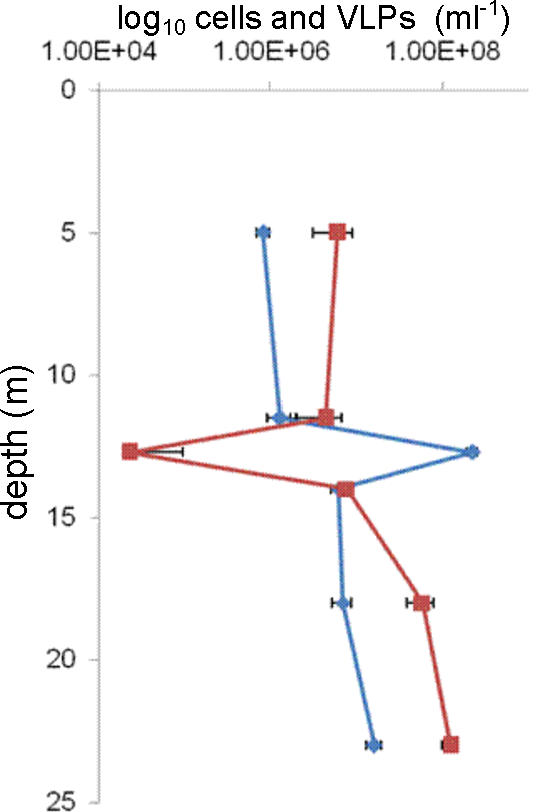
\includegraphics[width=50mm]{ace_figures/ace_counts.pdf}
\caption[Counts of microbial cells and \acs{VLP}s in Ace Lake]{Counts of microbial cells (blue) and \acs{VLP}s (red) by epifluorescence microscopy along a depth profile of Ace Lake.
Error bars represent one standard deviation.
No \acp{VLP} were detected at 12.7 m depth and the value reported represent the detection limit of the counting procedure (\emph{i.e.} one \acs{VLP} detected in one field of view).
}
\label{fig:ace_counts}

\end{figure}

No Anodisc filters could be obtained for such a comparative analysis to validate its use in this study.
However, for the purposes of this study, which is to show the relative differences in morphotypes between sample depths and size fractions, this method was more than suitable.
Other groups have since shown it to be comparable. %read papers and put in discussion.


\subsection[Community stratification supported by cell and \ac{VLP} densities]{Size and depth stratification of the community supported by cell and \ac{VLP} densities}
Development of fluorescence microscopy methodology using 0.01 \textmu{}m pore-size polycarbonate filters for simultaneous cellular and viral counts shows:

1. Size fractionation procedure appeared effective.

2. Morphological differences supports stratification of the community.

3. Visualisation of the morphology supported the metagenomic data that saw size fractionated and taxonomically stratified community.

4. Virus to bacteria ratios can give important information about the community.

At 12.7m depth, the light levels, and the sharp transition in oxygen content and salinity (Fig. S2) favour the dominance of a very high-density (2.2 $\times$ 10$^8$ cells ml$^{-1}$) of a single type of \ac{GSB} of the genus \emph{Chlorobia}, refered to as C-Ace \cite{Ng2010a}. 
Viral signatures were essentially devoid in this zone. 
The ratio of bacteriophage to total viral population increased proportionally in the larger size fractions consistent with trophic analyses that indicate that the larger size fractions are mostly copiotrophic (Fig. S8) particle attached bacteria and therefore likely to be sensitive to lysogenic phage infection \cite{Lauro2009}. 
The 23 m unfiltered lake water contained very high levels (1.3 $\times$ 10$^8$ \acp{VLP} ml$^{-1}$) of \acp{VLP}. 
The high diversity of bacteria and archaea in all size fractions of the monimolimnion (Fig. 2) is consistent with the presence of a high viral population (Rodriguez-Valera et al., NRM, 2009).


\subsection{Development of metaproteomic methodology}

1. Using a matched metagenome instead of \ac{NR} for protein identification greatly increased the number of identifications.
1.1 Except at the bottom zone, likely because the community is too diverse so greater coverage of the metagenome is required. %see available good spectra vs good reads
In parallel with taxonomic diversity increasing with depth (with the exception of the GSB layer), the rate of metaproteomic identification of proteins decreased with depth (Table S2). 
The majority of the proteins that were detected (e.g. 67\% at 23 m) were for hypothetical proteins that tended to lack orthologues in well-characterized organisms, highlighting both the functional importance and novelty of this anaerobic zone of the lake.


2. More specific information could be assigned to the taxonomic groups such as.
2.1. The Actinobacteria sequences in the mixolimnion were associated with a diverse phylogenetic cluster (Luna cluster) mainly contributed by freshwater ultramicrobacteria \cite{Hahn2003}. 
Several Luna cluster isolates contain rhodopsin genes \cite{Sharma2009} and similar gene sequences were present in the Ace Lake oxic zone data and found to be expressed (167820670 and 163154474; Table S2).
2.2.This is consistent with the identification of \ac{CRISPR} associated \ac{CAS} proteins Cse2, Cse3 and Cse4 (165526330, 165526332 and 165526334, respectively) in the 12.7 m metaproteome (Table S2). 
The \ac{CAS} gene locus (cas3, cse1, cse2, cse3, cse4, cas5, cas1b), to which the proteins map, shares its organisation with \ac{CAS} loci of sequenced \ac{GSB}, and groups with the \emph{E. coli} subtype/variant 2. The \ac{CRISPR}/\ac{CAS} system is likely to confer phage resistance to C-Ace, akin to the role in other organisms (Karginov and Hannon 2010; Horvath and Barrangou 2010).
%Recall that GSB all have large CRISPR regions and that the one in C-ace appears to be much reduced. Could this imply a lessening of viral load? The intervening spacers do not match to known viral sequences
% but did match to other GSB, could they be for competition?

3. Using \textsc{Scaffold} to validate protein identification and perform spectral counts was helpful. 
3.1Same protein identifications as Charmaine except one or two.
3.2 Able to quantify differences between mixolimnion and monimolimnion.
The diversity and abundance of \ac{ABC} transporters was lowest in the 0.1 \textmu{}m fractions at 23 m (Fig. 3), and a correspondingly low number were detected in the metaproteome (Table S2). 
In contrast, numerous transporters, predominately \ac{ABC} type, were identified in the metaproteome of the mixolimnion samples, with a high \ac{COG} representation of transporters for carbohydrates ($\sim$34\% of normalised spectra), amino acids ($\sim$32\%) and inorganic ions ($\sim$9\%) (Table S2 and Fig. S11).
All transporters in the metaproteome were of bacterial origin and conservative phylum level assignments of the normalised spectra showed the majority to originate from \emph{Proteobacteria} (69\%), 
of which SAR11 comprised 46\% and \emph{Actinobacteria} 19\% (Table S2). 
A high proportion of expressed genes with transport functions have also been reported for SAR11 from coastal (Poretsky et al. 2010) and open ocean waters (Sowell et al. 2009) (Morris et al. 2010?). 
Oligotrophs, such as SAR11 not only posses a low-diversity of high-affinity transporters (Lauro et al., 2009), but regulate the relative abundance of transporters expressed in response to \ac{DOC} availability (Poretsky et al. 2010). 
The prevalence of amino acid and simple sugar transporters (Table S2), and the low \ac{DOC} concentration in the Ace Lake mixolimnion (Fig. 1) is likely to reflect efficient utilisation of these substrates from the \ac{DOC} pool. 
Two SAR11 transport proteins that were detected in Ace Lake (Table S2) were not detected from the Sargasso Sea (Sowell,et al. 2009): an ectoine/hydroxyectoine (167807477 and 167892279) and a zinc \ac{ABC} transporter (167933120). The zinc \ac{ABC} transporter is likely to support zinc efflux in response to zinc concentrations which are $\sim$70-fold higher in the mixolimnion of Ace Lake compared to seawater (Rankin 1999). 
Conversely, phosphate transporters were a major class detected from the Sargasso Sea (Sowell,et al. 2009) but were absent from the Ace Lake metaproteome; consistent with lower phosphate levels in the Sargasso Sea ($<$5 nM) compared to Ace Lake (1--12 \textmu{}M). The differences in transporter expression between Ace Lake and oceanic SAR11 are likely to signify adaptive growth strategies that have evolved in the Ace Lake SAR11 community.
The high numbers of bacteriophages in the monimolimnion (detected by microscopy, Fig. S5 and S6; metaproteomics, Table S2; metagenomics, Fig. 2), and increase in \ac{DOC} observed at depth (Fig. 1), also indicates that carbon turnover in the monimolimnion is likely to be tightly coupled to the carbon flux going through a viral shunt, as proposed for open ocean systems (Suttle, C. A. Viruses in the sea. Nature 437, 356–361 (2005)). 
The bacteriophages are also likely vehicles for mediating gene exchange.
Most of the genetic potential to cycle the nitrogen pool appears to be limited to nitrogen assimilation throughout the lake and remineralisation in the monimolimnion (Fig. S14). 
The detection of glutamine synthetase (GlnA) and glutamate synthases (GltBS) in the metaproteome (Table S2) are supportive of active nitrogen assimilation. 
In the mixolimnion, GlnA was linked to SAR11 and \emph{Actinobacteria}, and they are likely to be responsible for nitrogen absorption in the oxic zone. At the oxycline, GlnA and GltB from GSB were abundant (Table S2), indicating an important role for nitrogen assimilation at this zone in the lake.
Genes for \ac{ASR} were present in metagenome data of all three fractions at all depths, although they were lowest at the oxycline. 
However, there was no evidence for expression of the genes as ASR proteins were not detected by metaproteomics. In contrast, multiple subunits of the GSB dissimilatory sulfide reductase complex were identified (Ng et al. 2010 and Table S2) indicating functionality of this pathway at the oxycline. 
\ac{GSB} likely utilise the dissimilatory sulfide reductase system to convert sulphur to sulfite and the polysulfide-reductase-like complex 3 to oxidize sulfite to sulphate. 
SRB may then reform sulphide completing the sulphur cycle between the \ac{GSB} and \ac{SRB} (Ng et al. 2010). 
While \ac{SRB} were detected at the three depths of the monimolimnion, sulphate is depleted in the water column and sediment at the bottom of the lake limiting their dissimilatory capacity \cite{Rankin1999}. 
Finally, sulphate in the mixolimnion can be linked to sulphur-oxidation by SAR11 (Meyer and Kuever, Microbiology 153:3478-3498) and a concomitant lack of capacity to perform sulphur reduction. 


%--------------------------------------------------------------------------------------------
\section{Conclusions}
Using complementary approaches helps to validate the research methodology and 
metagenomic inferences about the whole community.
Specifically, differences in size and depth was shown by both microscopy and metagenomics to be apparent.
This both validates the method of size fractionation as a viable approach to broad separation of the community,
as well as supports the assertion that there was a large difference in community at different depths.
Using a matched metaproteomic database showed a huge increase in the number of protein identifications.
This was provided that metagenomic coverage was good.
Using a metaproteomics, genes identified as potentially relevant in the metagenome were found to be expressed, supporting their importance.
For example, it showed the \ac{CRISPR} genes were active and may be a defence against phage.
It also showed Actinorhodopsins were expressed.
It showed that abundant genes were normally abundant in the metaproteome, such as transport proteins that give insight into what substrates are important components of the \ac{DOC} pool.
New inferences could be drawn from the metaproteome, such as the preference for labile substrates such as active sulfate reduction which is not apparent from the sulphate concentration.



%--------------------------------------------------------------------------------------------

\chapter{Virophage Control of Antarctic Algal Host--Virus Dynamics}
\label{ch:olv}

%-----------------------------------------------------------------------------------------------------
\section*{Co-authorship Statement}
\addcontentsline{toc}{section}{Co-authorship Statement}

A version of this chapter has been published as:\\

\textbf{Sheree Yau}, Federico M. Lauro, Matthew Z. DeMaere, Mark V. Brown, Torsten Thomas,
Mark J. Raftery, Cynthia Andrews-Pfannkoch, Matthew Lewis, Jeffery M. Hoffman, John A. Gibson, and
Ricardo Cavicchioli (2011)
Virophage control of antarctic algal host--virus dynamics.\\
\textit{\underline{Proceedings of the National Academy of Sciences USA}}
\textbf{108}: 6163--6168.\\

Contributions to this publication by other researchers is as follows.
Research was designed by Federico Lauro, Mark Brown, Torsten Thomas, John Gibson and Ricardo Cavicchioli.
Sample collection was performed by Federico Lauro, Mark Brown, Torsten Thomas, Jeffery Hoffman and Ricardo Cavicchioli.
DNA extraction and clone library preparation of 2006 samples was performed by Cynthia Andrews-Pfannkoch and Jeffery Hoffman of the J. Craig Venter Institute.
DNA sequencing quality control was performed by Matthew Lewis of the J. Craig Venter Institute.
Metagenomic sequence processing, global assembly and annotation was performed by Matthew DeMaere.
Assistance in mass spectronomy and mass spectra analysis was provided by Mark Raftery.
Assistance in analysis of Eucarya taxonomy was provided by Mark Brown.
Analysis of virophage abundance over time was performed by Federico Lauro.

Apart from these contributions, I performed all other data analyses and interpretations.
\newpage

%----------------------------------------------------------------------------------------------

\section{Abstract}

Viruses are abundant ubiquitous members of microbial communities, and in the marine environment affect population structure and nutrient cycling by infecting and lysing primary producers. 
Antarctic lakes are microbially dominated ecosystems supporting truncated food webs where viruses exert a major influence on the microbial loop. 
Here we report the discovery of a new virophage (relative of the recently described Sputnik virophage) that preys on phycodnaviruses that infect prasinophytes (phototrophic algae). 
By performing metaproteogenomic analysis on samples from Organic Lake, a hypersaline meromictic lake in Antarctica, complete virophage and near-complete phycodnavirus genomes were obtained. 
By introducing the virophage as an additional predator of a predator-prey dynamic model we determine that the virophage stimulates secondary production through the microbial loop by reducing overall mortality of the host and increasing the frequency of blooms during polar summer light periods. 
Virophages remained abundant in the lake two years later, and were represented by populations with a high level of major capsid protein sequence variation (25--100\% identity). 
Virophage signatures were also found in neighbouring Ace Lake (in abundance), and in two tropical lakes (hypersaline and fresh), an estuary, and an ocean upwelling site. 
These findings indicate that virophages regulate host-virus interactions and influence overall carbon flux in Organic Lake, and play previously unrecognised roles in diverse aquatic ecosystems.
\newpage

%---------------------------------------------------------------------------------------------

\section{Introduction}
It has been known for at least 20 years that viruses frequently infect and lyse marine primary producers causing up to 70\% of cyanobacterial mortality \cite{Proctor1990,Suttle1990}.
Eucaryotic phytoplankton are preyed upon by large dsDNA phycodnaviruses (PVs) causing bloom termination in globally distributed species (3,6).
Elevated levels of dissolved organic carbon (DOC) (7) and numbers of heterotrophic bacteria (8-10) occur during algal blooms indicating that viral lysis of eucaryotic algae stimulates secondary production. 
Viruses also suppress host populations at concentrations below bloom-forming levels, with abundance being controlled by the efficiency and production rates of the infecting viruses (11, 12). 

Antarctic lakes are microbially dominated ecosystems supporting few, if any metazoans in the water column (13, 14). 
In these truncated food webs, viruses are expected to play an increased role in the microbial loop (15). 
Low complexity Antarctic lake systems are amenable to whole community based molecular analyses where the role that viruses play in microbial dynamics can be unravelled (14). 
Attesting to this, a metagenomic study of Lake Limnopolar, West Antarctica uncovered a dominance of eucaryotic viruses and ssDNA viruses previously unknown in aquatic systems (16). 

We established a metaproteogenomic program for Organic Lake (68$^{\circ}$27$'$23.4$''$S, 78$^{\circ}$11$'$22.6$''$E), which is located in the Vestfold Hills, East Antarctica, in order to functionally characterize its microbial community. 
Organic Lake is a shallow (7 m) hypersaline ($\approx$230 g L$^{-1}$ maximum salinity) meromictic lake with a high concentration of dimethylsulphide ($\approx$120 $\mu$g $^{-1}$) in its anoxic monimolimnion (17, 18). 
Water temperature at the surface of the lake can vary from $-$14 to $+$15$^{\circ}$C while remaining sub-zero at depth (19, 20). 
The lake is eutrophic, with organic material sourced both from autochthonous production and input from penguins and terrestrial algae. 
The high concentrations of organic material reflect slow breakdown in the highly saline lake water. 
The salt in the lake was trapped along with the marine biota when the lake was formed due to falling sea level c. 3,000 y BP (21, 22). The lake sediment has both low species diversity (Shannon-Weaver diversity: 1.01) and richness (Chao non-parametric index: 32 $\pm$ 12) (23). 
Unlike high latitude lakes, viral abundance has been reported to increase with trophic status (15) and with salinity in Antarctic lakes (24). 

Here we report the analysis of the surface water of Organic Lake, highlighting the presence of a relative of the recently described Sputnik virophage, a small eucaryotic virus that requires a helper \textit{Acanthamoeba polyphaga} mimivirus (APMV) to replicate (25). 
From metagenomic DNA, a complete Organic Lake virophage (OLV) genome was constructed (the second virophage genome to be described), and near-complete genomes of its probable helper Organic Lake phycodnaviruses (OLPVs).

%------------------------------------------------------------------------------------------

\section{Materials and Methods}

\subsection{Samples and DNA Sequencing}
Water samples collected from Organic Lake were: 

\begin{enumerate}
\item Surface water from the eastern side of the ice-free lake (68$^{\circ}$27$'$25.48$''$S, 78$^{\circ}$11$'$28.06$''$E) December 24, 2006.
\item A depth profile collected through a 30 cm hold drilled through the surface ice above the deepest point in the lake (68$^{\circ}$27$'$22.15$''$S, 78$^{\circ}$11$'$23.95$''$E), November 10, 2008. 
\item surface water from the north-east side of the partially ice-covered lake (68$^{\circ}$27$'$21.02$''$S 78$^{\circ}$11$'$42.42$''$E), December 12, 2008. 
\end{enumerate}

Samples were sequentially filtered through a 20 $\mu$m pre-filter and biomass captured onto 3.0, 0.8 and 0.1 $\mu$m membrane filters as described previously (1, 2). 
The samples from 2008 also included 50\% (v/v) RNAlater. 
DNA extraction, sequencing and quality validation was performed as previously described (1, 2). 
DNA sequencing was performed at the J. Craig Venter Institute in Rockville, MD, USA.  

\subsection{Transmission Electron Microscopy}
Unfiltered Organic Lake surface water from December 24, 2006 (fixed on-site in 1\% (v/v) formalin) was concentrated and a solvent exchange performed with sterile filtered ammonium acetate solution 1\% (w/v) using a 50 kDa cut-off Microcon centrifugal filter device (Millipore) according to the manufacturer’s instructions. 
Formvar coated 200 mesh copper grids were floated on a droplet of sample for 30 min, excess liquid wicked off and the grid negatively stained for 30 s with uranyl acetate 2\% (w/v). 
The sample was visualised using a JEOL1400 transmission electron microscope at 100 kV at 150,000 to 250,000 $\times$ magnification.

\subsection{Metagenomic Assembly and Annotation}
Mosaic metagenomic assemblies were generated as previously described (1, 2). 
For the 0.1 $\mu$m Organic Lake 2006 sample, assembly was a hybrid of Sanger and 454 read data (Table S1). 
For all other sample size fractions, runtime parameters used were standard for 454 sequencing data. 
Low GC ($\ge$ 51\%) scaffolds $>$ 10 kb from the 0.1 $\mu$m 2006 assembly had high coverage ($>$ 45 $\times$) indicating these were from the dominant taxa. 
One of these scaffolds was binned as virophage and the rest as PV. 

To further separate the OLPV types and assess the completeness of their genomic content, highly conserved single copy PV orthologues were identified as follows. 
An all against all BLASTp search was conducted with protein sequences from the ten available PV genomes 
(\textit{Acanthocystis turfacea Chlorella} virus 1, PbCV-1, PbCV AR158, PbCV FR483, PbCV NY2A, \textit{Emiliania huxleyi} virus 86, \textit{Ectocarpus siliculosus} virus 1, \textit{Feldmannia} sp. virus, \textit{Ostreococcus} virus 5, \textit{Ostreococcus tauri} virus 1) and APMV (which was included as a close PV relative). 
BLASTp results were parsed and clustered using orthoMCL V1.4 (3, 4). 

Pairs of each orthologue were located on eight of the PV scaffolds. 
The location of each orthologue pair had a complementary distribution so the eight scaffolds were able to be sorted unambiguously into two strains (OLPV-1 and OLPV-2). 
OLPV-1 ribonucleotide reductase $\alpha$-subunit appeared as duplicated on different scaffold ends, likely as an artefact of its proximity to an assembly break point. 
The remaining high coverage scaffolds were searched for predicted proteins present in one OLPV strain but not in the other and assigned to the strain in which it was absent. 
Comparison of OLPV-1 and OLPV-2 scaffolds was performed using tBLASTn of concatenated scaffolds from each strain and visualised using the Artemis Comparison Tool (ACT) (5). 
DNA sequence data is available in Genbank and CAMERA (http://web.camera.calit2.net).

\subsection[Genome Completion and Annotation]{Organic Lake Virophage Genome Completion and Annotation}
The high coverage (77 $\times$), large number of Sputnik homologues that encode essential functions and length of the putative OLV scaffold from the 0.1 $\mu$m 2006 hybrid assembly indicated it was a near-complete genome. 
Reads from this scaffold were reassembled at high stringency and visualised using Phred/Phrap/Consed (6) to complete the sequence. 
Mate-pair data indicated a circular molecule and primers were designed to span the ends of the scaffold and sequence across the gap (Table S5). 
Touch-down PCR was performed with eDNA from 0.1 $\mu$m 2006 sample, the product used for nested PCR and the final product was cloned and sequenced. 
The complete genome was manually annotated and visualised using Artemis (7). 
Translated ORFs (minimal size 120 amino acids) were compared (BLASTp) to GenBank, to the all metagenomic ORF peptide database on CAMERA (http://web.camera.calit2.net) and to predicted proteins from OLPV-1 and OLPV-2 scaffolds. 
Comparisons between the OLV genome and OLPV-1 /OLPV-2 were performed with tBLASTn and visualised using ACT (5). 

\subsection{Phylogenetic Analysis}
Translated amino acid sequences from viral marker genes of interest were retrieved from the 0.1 $\mu$m 2006 metagenomic assemblies from this study, GenBank and CAMERA all metagenomic reads ORF peptide database. Homologous sequences were aligned using MUSCLE v3.6 (8). 
Neighbour-joining analysis, test for clade support (bootstrap analysis 2000 replicates) and tree drawing was performed with Molecular Evolutionary Genetics Analysis (MEGA) software v4 (9). 
Maximum likelihood analysis (JTT substitution model) and test for clade support (aLRT analysis) was performed with PhyML (10) and the tree visualised using MEGA. 
18S rRNA gene sequences were retrieved from reads of all filter sizes, compared (BLASTn, e-value $<$ 1.0e$-$5) to the SILVA100 SSURef database, aligned and phylogeny performed using ARB as previously described (1, 2). 
The abundance and similarity of virophages in all lake samples and filter sizes was estimated using BLASTp (evalue $<$ 1.0e$-$5) to search using the OLV MCP sequence against a database of proteins predicted from sequencing reads. 
The database was generated as previously described (1) and the percent identity of the BLAST hit was used as a proxy for species similarity. 

\subsection{Metaproteomic Analysis}
Metaproteomics of proteins from the 0.1 $\mu$m filter from 2006 was performed as previously described (1, 2), with minor modifications. 
The protein sequence database was generated by combining ORFs from the 3.0, 0.8 and 0.1 $\mu$m mosaic assemblies with 130,581 sequences in the database. 
Scaffold 3.0 (Proteome Software Inc.) was used to validate MS/MS based peptide and protein identifications. 
Protein identification data is available in Table S2. 

\subsection[Algal Host--Virus and Virophage Dynamics]{Model of Algal Host--Virus and Virophage Dynamics}
To model the effect a virophage would have on algal Pyramimonas algal host populations in Organic Lake, modified Lotka-Volterra equations were used describing the OLV as a predator of predator OLPV. 
The original equations are given by:

\begin{equation}
\frac{\mathrm{d}A}{\mathrm{d}t}=\alpha A - \varepsilon PA
\label{eqn:lokprey}
\end{equation}

\begin{equation}
\frac{\mathrm{d}P}{\mathrm{d}t}= \theta PA - \mu P
\label{eqn:lokpred}
\end{equation}

Where:
\begin{description}
\item[$A$] is the number of \textit{Pyramimonas} (prey).
\item[$P$] is the number of OLPV (predator).
\item[$\alpha$] is the specific growth rate of the prey.
\item[$\theta$] is the specific production rate of the predator.
\item[$\varepsilon$] is the rate of predator mediated death of prey.
\item[$\mu$] is the specific decay rate of the predator.
\end{description}

Equation \ref{eqn:lokprey} describes the change in \textit{Pyramimonas} abundance and equation \ref{eqn:lokpred} the change in OLPV abundance in the absence of OLV.
In the presence of OLV, \textit{Pyramimonas}, OLPV and OLV dynamics are described by the following equations:

\begin{equation}
\frac{\mathrm{d}P}{\mathrm{d}t}= \theta PA - \mu P - \omega PV
\label{eqn:pred}
\end{equation}
\begin{equation}
\frac{\mathrm{d}V}{\mathrm{d}t}=\beta PV - \gamma V
\label{eqn:viro}
\end{equation}

Where:
\begin{description}
\item[$V$] is the number of teh OLV (predator of predator).
\item[$\omega$] is the rate of OLV mediated reduction in OLPV infective particles.
\item[$\beta$] is the production rate of OLV.
\item[$\gamma$] is the decay rate of OLV.
\end{description}

Equation \ref{eqn:pred} is a modified version of equation \ref{eqn:lokpred} which includes the effect of OLV on the change in abundance of OLPV.
Equation \ref{eqn:viro} describes the growth properties of OLV as a predator of OLPV.
Values for the variables for the solution shown (Fig. 4) were as follows: initial prey (10), predator (1) and predator of predator (10) numbers, ~$\alpha=$ 0.1, ~$\theta=$ 0.0015, ~$\varepsilon=$ 0.01, ~$\mu=$ 0.01, ~$\omega=$ 0.01, ~$\beta=$ 0.015 and ~$\gamma=$ 0.15. 
COmplex PAthway Simulator (COPASI) software (11) was used to simulate prey, predator and predator of predator dynamics using the deterministic (LSODA) method.
%-----------------------------------------------------------------------------------------


\section{Results and Discussion}
\subsection{Dominance of Phycodnaviruses in Organic Lake}
Water samples from Organic Lake were collected December 2006 and November and December 2008, and microbial biomass collected onto 3.0, 0.8 and 0.1 $\mu$m membrane filters as described previously (14). 
A large proportion of shotgun sequencing reads (96.2\%) from the 0.1 $\mu$m size fraction of the 2006 Organic Lake metagenome (Table S1) had no significant hits to sequences in the RefSeq database 
(tBLASTx with e-value $<$ 1.0e$-$3, minimum alignment length: 60 bp, minimum identity: 60\%). 
The degree of assembly was high, with 77\% of reads forming part of a scaffold, indicating the sample contained a few abundant taxa of minimal diversity. 
Forty-five scaffolds were longer than 10 kb; the five longest ranged from 70 to 171 kb. 
GC content and coverage were used to separate scaffolds into taxonomic groups (Fig. S1). 
A broad division was evident between low ($\le$ 41\%) and high ($\ge$ 51\%) GC scaffolds suggesting they constituted two taxonomic groups. 
All scaffolds in the high GC group that could be assigned contained phage homologues, as did the one exceptional low GC scaffold. 
The low coverage in the high GC group showed bacteriophages were not abundant in the 0.1 $\mu$m fraction. 
These scaffolds were not analyzed further. 
The low GC scaffolds with confident assignments contained sequences matching conserved PV or APMV proteins. 
These PV-related scaffolds comprised 60\% of assembled reads demonstrating that OLPVs were numerically dominant in the 0.1 $\mu$m fraction. 
Transmission electron microscopy (TEM) revealed the presence of virus-like particles with the dimensions and structure typical of PVs (Fig. 1A).

Within the low GC group, scaffolds separated into a high coverage ($>$ 45$\times$) group, including the five longest scaffolds, and a low coverage ($<$ 22$\times$) group. 
Two of the scaffolds in the high coverage group and one in the low coverage group contained the PV marker DNA polymerase B (DPOB). 
The two high coverage DPOB share 76\% amino acid identity and both share ~$\approx$57\% identity to the low coverage DPOB. 
DPOB is single-copy throughout the nucleo-cytoplasmic large DNA virus (NCLDV) family to which PVs belong (26,27), 
demonstrating that the Organic Lake surface waters contained two closely related abundant PV types (DPOB1) and (DPOB2), and a more distantly related lower abundance type (DPOB3). 

Phylogenetic analysis clustered Organic Lake DPOB with unclassified lytic marine PV isolates that infect the prymnesiophytes \textit{Chrysochromulina ericina} (CeV1) and \textit{Phaeocystis pouchetii} (PpV),
 the prasinophyte \textit{Pyramimonas orientalis} (PoV) (4,28), and uncultured marine PVs related to APMV (29, 30) (Fig. 2A and Fig. S2). 
As the host range of PVs broadly correlates with DPOB phylogeny (31, 32), OLPV would infect prasinophytes or prymnesiophytes. 
The most probable host is the prasinophyte, \textit{Pyramimonas} (no prymnesiophyte 18S rRNA gene sequences were present in any size fraction of the Organic Lake metagenome) (Fig. S3).

Supporting the presence of more than one PV, pairs of single-copy PV orthologues 
(ribonucleotide reductase alpha and beta subunits, VV A32R virion packaging helicase, PBCV1 A482R-like putative transcription factor, VV D5 ATPase and VLTF2 family transcription factor) 
were identified in the high coverage scaffolds that shared an average of 81\% percent amino acid identity.
 Based on the positions of single copy genes on the scaffolds and the percent identity between them, the high coverage scaffolds were grouped into two strains designated OLPV-1 and OLPV-2 according to their DPOB phylogeny (Fig. 2A and Fig. S2).
 The remaining high coverage scaffolds were assigned to either strain, resulting in two near-complete genomes of $\approx$300 kb each (Fig. 2C), 
that are within the range of other sequenced PV genomes (155-407 kb). 
In addition, several OLPV genomic fragments contained PV homologues in high coverage scaffolds that could not be confidently assigned to either strain. 

Both OLPV strains contain a PpV-like major capsid protein (MCP) designated MCP1 and another unique MCP designated MCP2 (Fig. 2B and Fig. S4). 
Both OLPV MCP1s were identified in the metaproteome (Fig. 2C and Table S2) but MCP2 was not. 
In addition to MCPs, the metaproteome contained a range of abundant structural proteins and others more likely to be packaged in the virion (e.g. chaperone), that were expressed by OLPV-1, OLPV-2 and/or an OLPV genomic fragment (Fig. 2C and Table S2). 
These data suggest that MCP1 is the major structural protein, and that both OLPV-1 and OLPV-2 were in a productive cycle in the lake at the time of sampling. 

\subsection{Complete Genome of an Organic Lake Virophage}
Sputnik is a small (50 nm) icosahedral satellite virus of mamavirus (a new strain of APMV). 
It was termed a ``virophage'' because co-infection with Sputnik is deleterious to the mamavirus, resulting in abnormal virions and a decrease in mamavirus infectivity (25). 
One 28 kb scaffold in the low GC high coverage group had six out of 38 predicted proteins homologous to Sputnik virophage proteins (Fig. 3 and Table S3), and one PV homologue. 
The scaffold had a low GC content (~$\approx$30\%), similar to the Sputnik genome, and was larger in size (28 kb vs 18 kb for Sputnik). 
Using PCR and sequencing, the scaffold was found to represent a complete circular virophage genome (the Sputnik genome is also circular). Virus-like particles resembling Sputnik in size and morphology were identified by TEM (Fig. 1B).

Sputnik homologues present in the Organic Lake scaffold included the V20 MCP, V3 DNA packaging ATPase, V13 putative DNA polymerase/primase and others of unknown function (V9, V18, V21 and V32) (Fig. 3 and Table S3). 
The Organic Lake virophage (OLV) is distinct to Sputnik as proteins share 27-42\% amino acid identity (28\% MCP identity). 
OLV proteins include OLV9, the homologue of Sputnik V20 MCP, and OLV8, a fusion of the uncharacterised V18 and minor virion protein V19 from Sputnik (Fig. 3 and Table S3). 
The large number of homologues, including genes that fulfill essential functions in Sputnik (V20, V3 and V13), indicate that OLV and Sputnik have physiological similarities. 

\subsection{Gene Exchange Between Virophage and Phycodnaviruses}

As PVs are related to APMV (27) and are abundant in Organic Lake, it stands to reason that OLPV is the helper of OLV. 
In the OLV genome, OLV12 is a \textit{Chlorella} virus-derived gene, indicating that gene exchange has occurred between OLV and PVs (the function of OLV12 is discussed below). 
Similar observations were made for Sputnik, which carries four genes (V6, V7, V12 and V13) in common with the mamavirus, indicative of gene exchange between the viruses and possible co-evolution (25). 
As the V6, V7, V12 and V13 proteins have been associated with virophage-helper specificity, we reasoned that the functional analogues in OLV would have highest identity to proteins from its helper virus, rather than Sputnik. 

By comparing OLV and OLPV, a 7,408 bp region was identified in OLV encoding five proteins (OLV17-22) with identity (32--65\%) to sequences in both OLPV-1 and OLPV-2 (Fig. 2C, Fig. S5 and Table S3). 
OLV20 and OLV13 are collagen triple-helix-repeat-containing proteins, analogous to Sputnik collagen-like proteins (V6 and V7) involved in protein-protein interactions in the APMV virus factory. 
Sputnik can replicate with either mamavirus or APMV as a helper, although coinfection rates are higher with the mamavirus. 
V6 is the only protein with higher identity (69\%) to mamavirus than APMV (42\%) (25). 
Since OLV20 has equivalent identity (63\%) with OLPV-1 and OLPV-2, it appears that OLV may be capable of interacting with both OLPV strains. 
Also within the conserved region, OLV22, is a 141 aa protein of unknown function that only matches sequences from OLPV and the Global Ocean Sampling (GOS) expedition (Table S3). 
Similar to OLV22, Sputnik V12 is a small protein (152 aa) of unknown function with high identity to APMV, and both may mediate a specific helper-virophage interaction. 
Other genes in this region of OLV can be mapped to OLVP, including a putative transmembrane protein (OLV17) and paralogous phage tail fibre repeat containing proteins, OLV18 and OLV19. 
Analogous to the collagen-like proteins, OLV19 and OLV20 probably facilitate interactions between helper and virophage. 

OLV12 (which is unique to OLV) consists of a C-terminal domain present in conserved hypothetical \textit{Chlorella} virus proteins and an N-terminal domain most closely related to class 3 lipases that may confer OLV selectivity to a PV. 
OLV12 may function similarly to the Sputnik V15 membrane protein in modifying the APMV membrane (25). 
The Sputnik V13 consists of a primase domain and SF3 helicase domain related to NCLDV homologues, involved in DNA replication. 
The helicase domain of OLV25 and V13 are similar, although the primase domain is more similar to a protein from \textit{Ostreococcus lucimarinus}, implying a past association of OLV with a prasinophyte alga host. 

Genes unique to OLV point to adaptations specific to its helper-host system. 
Most notably, OLV possesses a N6 adenine-specific DNA methyltransferase, as does OLPV. 
In OLPV-1, genes for a bacterial type I restriction modification (RM) system are adjacent to a gene encoding a type I methylase-S target recognition domain protein, and upstream of a DNA helicase distantly related to type III restriction endonuclease (RE) subunits. 
A large number of \textit{Chlorella} virus genomes have both 5mC and 6mA methylation (33), and several contain functional RM systems (34). 
The prototype \textit{Chlorella} virus PbCV-1 possesses REs packaged in the virion for degrading host DNA soon after infection (35). 
In contrast to OLV/OLPV, DNA methyltransferases are absent in both Sputnik and APMV, indicating that the N6 adenine-specific DNA methyltransferase has been selected in OLV to reduce endonucleolytic attack mediated by OLPV. 

\subsection[Virophage in Algal Host--Phycodnavirus Dynamics]{Role of Virophage in Algal Host--Phycodnavirus Dynamics}
The presence of the virophage adds an additional consideration to the microbial loop dynamics. 
In batch amoeba cultures, co-infection of amoeba with APMV and Sputnik causes a 70\% decrease in infective AMPV particles and a 3-fold decrease in lysis (25). 
To test how OLV affects OLPV and host population dynamics, we modelled the OLV as an additional predator of a predator in a Lotka-Volterra simulation (Fig. 4). 
In the model, the effect of virophage is robust, with equilibrium solutions across a wide range of parameter values (Fig. 4 shows one equilibrium solution). 
By decreasing the number of infective OLPVs, the presence of OLV shortens the recovery time of the host population (Fig. 4C) and shifts the orbit away from the axis (Fig. 4D). 
The model reveals that the virophage stimulates the flux of secondary production through the microbial loop by reducing overall mortality of the host algal cell following a bloom, and by increasing the frequency of blooms during the summer light periods. 
Antarctic lake systems have evolved mechanisms to cope with long light-dark cycles (14) and shortened trophic chains. 
In Organic Lake and similar systems, a decrease in PV virulence may be instrumental in maintaining stability of the microbial food web. 

\subsection{Ecological Relevance of Virophages in Aquatic Systems}
Metagenomic analysis of Organic Lake samples taken two years later in November (when the lake was ice covered) and December 2008 (partially ice-free) revealed sequences with 99\% amino acid identity to OLV MCP indicating persistence of OLV in the ecosystem (Fig. 5 and Table S4). 
In addition, sequences with lower identity (25--90\%) were detected, particularly in December, demonstrating Organic Lake virophages are highly diverse but OLV remained the dominant type. 

From surface water samples of nearby Ace Lake (meromictic, surface 2\% salinity), a large number of sequences were obtained that matched both the OLV MCP (Fig. 5 and Table S4) and PVs (14). 
All Ace Lake size fractions contained matches to OLV MCP, some with high identity (80--100\%) and the majority with greater variation (25--80\% identity) (Fig. 5 and Table S4). 
In contrast to Organic Lake where the largest number of matches was to the 0.1 $\mu$m size fraction, the majority of Ace Lake sequences were from the larger fractions (Fig. 5 and Table S4). 
This indicates the Ace Lake virophages were associated with host cells during sampling, or possibly with helper viruses that are larger than the OLPVs. 

Extending the OLV MCP search to the GOS data revealed matches (25-28\% identity) to sequences from the hypersaline Punta Cormorant Lagoon (Floreana Island, Galapagos), an oceanic upwelling near Fernandina Island (Galapagos), Delaware Bay estuary (NJ, USA), and freshwater Lake Gatun (Panama) (Table S4). The phylogenetic analysis of a conserved 103 amino acid region of the MCPs revealed a number of clusters, with Sputnik clustering with virophage sequences from Ace Lake that had low identity (22\%) to OLV MCP (Fig. 5 and Fig. S4). 
To improve searches for virophages and better understand their physiology and evolution, it will be valuable to target more genomes (e.g. the Ace Lake 167858124 relative with 40\% MCP identity to Sputnik) and determine which genes are core to virophages and what relationship exists between genome complement and MCP identity.
 
In view of the implications of the virophage modelling (Fig. 4), the abundance and persistence of OLV in Organic Lake (Fig. 5, Table S4), and the presence of diverse virophage signatures in a variety of lake systems (fresh to hypersaline), an estuary, an ocean upwelling site and a water cooling tower (Sputnik), our study indicates that numerous types of virophages exist and play a previously unrecognised role in regulating host--virus interactions and influencing ecosystem function in aquatic environments. 

%------------------------------------------------------------------------------------------------------

\section{Acknowledgements}
We thank Craig Venter, John Bowman, Louise (Cromer) Newman, Anthony Hull, John Rich and Martin Riddle for providing helpful discussion and logistical support associated with the Antarctic expedition, and Lisa Ziegler for discussion about marine viruses. 
We acknowledge technical support for computing infrastructure and software development from Intersect, and in particular assistance from Joachim Mai. 
This work was supported by the Australian Research Council and the Australian Antarctic Division. 
Funding for sequencing was provided by the Gordon and Betty Moore Foundation to the J. Craig Venter Institute. 
Mass spectrometric results were obtained at the Bioanalytical Mass Spectrometry Facility within the Analytical Centre of the University of New South Wales. 
This work was undertaken using infrastructure provided by NSW Government co-investment in the National Collaborative Research Infrastructure Scheme. 
Subsidized access to this facility is gratefully acknowledged. 
We thank Jenny Norman from the UNSW Electron Microscopy Unit her assistance in generating images. 

\chapter{Strategies of carbonn conservation and unusual sulphur biogeochemistry in a hypersaline Antarctic Lake}
\label{ch:org}
\acresetall

%---------------------------------------------------------------------------------------------
\section*{Co-authorship Statement}
A version of this chapter has been submitted as:\\

\textbf{Sheree Yau}, Federico M. Lauro, Timothy J. Williams, Matthew Z. DeMaere, Mark V. Brown, John Rich, 
John A.E. Gibson, Ricardo Cavicchioli. 
Strategies of carbon conservation and unusual sulfur biogeochemistry in a hypersaline lake.
\emph{\underline{ISME Journal}}
submitted, 2013.

Contributions to this manuscript by other researchers is as follows.

Research was designed by Federico Lauro, Mark Brown, John Gibson and Ricardo Cavicchioli.
Sample collection was performed by Federico Lauro, Mark Brown and Ricardo Cavicchioli.
Metagenomic sequence filtering, global assembly and annotation was performed by Matthew DeMaere.
Assistance in intrepretation of functional potential provided by Timothy Williams.

Apart from these contributions, I performed all other data analyses and interpretations.
\newpage

%----------------------------------------------------------------------------------------------

\section{Abstract}
Organic Lake is a shallow, marine-derived hypersaline lake in the Vestfold Hills, Antarctica that has the highest reported concentration of dimethylsulphide \ac{DMS} in a natural body of water.
To determine the composition and functional potential of the microbial community and learn about the unusual sulphur chemistry in Organic Lake, shotgun metagenomics was performed on size fractionated samples collected along a depth profile.
Eucaryal phytoflagellates were the main photosynthetic organisms.
Bacteria were dominated by the globally distributed heterotrophic taxa \emph{Marinobacter}, \emph{Roseovarius} and \emph{Psychroflexus}.
The dominance of heterotrophic degradation coupled with low fixation potential indicates possible net carbon loss.
However, abundant marker genes for aerobic anoxygenic phototrophy, sulphur oxidation, rhodopsins and CO oxidation were also linked to the dominant heterotrophic bacteria and indicate use of photo- and lithoheterotrophy as mechanisms for conserving organic carbon.
Similarly, a high genetic potential for the recycling of nitrogen compounds likely functions to retain fixed nitrogen in the lake.
\ac{DMSP} lyase genes (\emph{dddD}, \emph{dddL} and \emph{dddP}) were abundant indicating \ac{DMSP} is a significant carbon and energy source.
Unlike marine environments, \ac{DMSP} demethylases (\emph{dmdA}) were less abundant than \ac{DMSP} lyases indicating that \ac{DMSP} cleavage is the likely source of the high \ac{DMS} concentration.
\ac{DMSP} cleavage, photoheterotrophy, lithoheterotrophy and nitrogen remineralisation by dominant Organic Lake bacteria are potentially important adaptations to nutrient constraints.
In particular, photo- and lithoheterotrophy reduces the extent of carbon oxidation for energy production allowing more carbon to be used for biosynthetic processes.
The study sheds light on how the microbial community in Organic Lake has adapted to the unique physical and chemical properties of this Antarctic Lake environment.

\newpage

%---------------------------------------------------------------------------------------------
\acresetall
\section{Introduction}
%Molecular biology approaches have proven useful for describing the diversity and gene content of microorganisms in Antarctic lakes and for inferring the functional roles of the taxa present \cite{Laybourn-Parry2007}.
%However to date, only a few large scale shotgun metagenome studies have been performed on the Antarctic continent and in the surrounding Southern Ocean \cite{Wilkins2012a}. 
%In the Vestfold Hills, metagenomics and metaproteomics have been used to study Ace Lake (68$^{\circ}$28$'$23.2$''$S, 78$^{\circ}$11$'$20.8$''$E) \cite{Ng2010a, Lauro2011} and Organic Lake (68$^{\circ}$27$'$23.4$''$S, 78$^{\circ}$11$'$22.6$''$E) \cite{Yau2010}.
%For Ace Lake, a comprehensive assessment of the community structure, biogeochemical fluxes and responses to resource limitation have been described \cite{Lauro2011}.
%The metabolism of abundant green sulphur bacteria \cite{Ng2010a} was found to play a central role in nutrient cycling and a mathematical model was developed that showed its dominance was dependent on synchronicity with the polar light cycle leading to absence of phage predation \cite{Lauro2011}.
%For Organic Lake, a member of the virophage virus family was discovered that potentially regulates microbial loop dynamics \cite{Yau2011}. 
%The Organic Lake virophage likely depends on phycodnaviruses (algal viruses) and it was predicted that the virophage would reduce infective phycodnaviruses leading to an increased frequency of algal blooms and thus carbon flux \cite{Yau2011}.
%Virophage sequences were also identified in a range of aquatic metagenomes revealing that they are likely to play ecologically important roles in many aquatic systems \cite{Yau2011}. 
%These studies on Ace and Organic lakes both used shotgun metagenomics and illustrate the value of adopting a metagenomics approach for learning about microbial ecology in Antarctic environments.
Due to the polar light cycle, phototrophic growth in Antarctic environments is relatively high in summer and negligible in winter \cite{Laybourn-Parry2005} and requires microbial life to survive under long periods under a scarcity of resources.
To overcome this limitation, Eucaryotic phytoflagellates in Ace Lake engage in carbon mixotrophy by grazing on bacterioplankton to supplement their carbon requirements in the winter \cite{Laybourn-Parry2005}.
Marine heterotrophic bacteria are known to be similarly resourceful by exploiting light energy through photoheterotrophy that includes \ac{AAnP} or via use of rhodopsins, or lithoheterotrophy such as oxidation of carbon monoxide \cite{Moran2007b}.
Heterotrophic bacteria that can harness energy sources apart from organic carbon can direct a greater proportion of carbon towards growth, which serves to conserve fixed carbon within a closed systems \cite{Moran2007b}. 

Organic Lake is shallow (6.8 m) and has variable surface water temperatures ($-$14 to $+$15$^{\circ}$C) while remaining sub-zero throughout most of its depth \cite{Franzmann1987b, Gibson1991, Roberts1993b, Gibson1999}.
The salt and marine biota in the lake originate from seawater that was trapped in a basin $\sim$3,000 BP \cite{Zwartz1998, Bird1991}. 
The bottom waters of Organic Lake are unusual due to the absence of hydrogen sulphide and the high concentration of the volatile gas \ac{DMS} \cite{Deprez1986, Franzmann1987b, Gibson1991, Roberts1993a, Roberts1993b}. 
Concentrations of \ac{DMS} as high as 5,000 nM have been recorded in Organic Lake \cite{Gibson1991}, 100 times the maximum concentration recorded from seawater in the adjacent Prydz Bay and at least 1 000 times that of the open Southern Ocean \cite{Curran1998}.
More than forty years ago atmospheric \ac{DMS} was proposed to have a regulatory effect on global cloud cover as it is a precursor of cloud condensation nuclei \cite{Lovelock1972, Charlson1987}.
However, the first enzymes involved in \ac{DMS} production were only identified in the last six years \cite{Todd2007}.
Rapid progress has been made in this short period and the pathways and organisms involved in \ac{DMS} transformations have been extensively reviewed \cite{Johnston2008, Schafer2010, Curson2011b, Reisch2011b, Moran2012}. 

The main source of \ac{DMS} in the marine environment is from the breakdown of \ac{DMSP}. 
Eucaryal phytoplankton, in particular diatoms, dinoflagellates and haptophytes, produce large quantities of \ac{DMSP}, an organosulphur compound that is thought to function principally as an osmolyte. 
\ac{DMSP} is released due to cell lysis, grazing or leakage and follows two known fates: \ac{DMSP} cleavage by \ac{DMSP} lyases (DddD, -L, -P, -Q, -W and -Y) or demethylation by \ac{DMSP} demethylase (DmdA).
 Both pathways are associated with diverse microorganisms that can utilize \ac{DMSP} as a sole carbon and energy source. 
However, it is only the cleavage pathway that releases volatile \ac{DMS} that can lead to sulphur loss through ventilation to the atmosphere.
The very high levels of \ac{DMS} in Organic Lake make it an ideal system for identifying the microorganisms and the processes involved in \ac{DMS} accumulation. 

The previous Organic Lake metagenomic study examined viruses from the 0.1 $\mu$m fraction of surface water that was collected from Organic Lake in December 2006, and November and December 2008 \cite{Yau2011}. 
In the present study we focused on the cellular population rather than viruses. 
Our study determined the composition and functional potential of Organic Lake microbiota and, in conjunction with historic and contemporary physico-chemical data, generated an integrative understanding of the whole lake ecosystem. 
%------------------------------------------------------------------------------------------

\section{Materials and methods}
\subsection{Characteristics of the lake and sample collection}
The water level of Organic Lake was measured by surveying as $+$1.886 m relative to the survey mark (NMV / S / 53) located at 68$^{\circ}$27$'$23.4$''$S, 78$^{\circ}$11$'$22.6$''$E.
Water was collected from Organic Lake on 10 November 2008 through a 30 cm hole in the 0.8 m thick ice cover above the deepest point in the lake. 
The sampling hole was established at 68$^{\circ}$27$'$22.2$''$S, 78$^{\circ}$11$'$23.9$''$E) following bathymetry measurements constructed on a metric grid. 
Samples were collected for metagenomics, microscopy and chemical analyses at 1.7, 4.2, 5.7, 6.5 and 6.7 m depths (maximum lake depth 6.8 m).

For metagenomics, lake water was passed through a 20 $\mu$m pore size pre-filter, and microbial biomass captured by sequential filtration onto 3.0 $\mu$m, 0.8 $\mu$m and 0.1 $\mu$m pore size 293 mm polyethersulfone membrane filters, and samples immediately preserved in buffer and cryogenically frozen in liquid nitrogen, as described previously \cite{Ng2010a, Lauro2011}. 
Between 1--2 L of lake water was sufficient to saturate the holding capacity of the filters. 
\ac{DNA} was extracted from the filters, samples sequenced using the Roche GS-FLX titanium sequencer, and reads processed to remove low quality bases, assembled and annotated, as previously described \cite{Ng2010a, Lauro2011}. 
A summary of the 2.4 Gbp of metagenomic data isprovided in Supplementary Table S1.

\subsection{Physical and chemical analyses}
An \emph{in situ} profile of pH, conductivity, turbidity, \ac{DO} and pressure was measured using a submersible probe (YSI sonde model V6600). 
A temperature profile was measured using a maximum-minimum mercury thermometer as the YSI probe did not have a capacity to record temperature below $-$10$^{circ}$C. 
The 5.7 m sample corresponded to the turbidity maximum and the 6.5 m sample to the turbidity minimum. 
Conductivity at \emph{in situ} temperature was converted to conductivity at 15$^{\circ}$C as described previously \cite{Gibson1999}. 
The adjusted conductivity brings the temperature to within a range suitable for estimating practical salinity using the formula of \citet{Fofonoff1983}. 
Salinity was likely to have been underestimated as it is higher than the range (2--42) for which the conductivity--salinity relation holds. 
However, the relative difference in salinity between the samples would be accurate. 

Density was calculated from the \emph{in situ} conductivity and temperature using the equations described by \citet{Gibson1990} and expressed at temperature T as:

\begin{equation}
\sigma_T = (1000 - density) kg m^{-3}
\label{eqn:density}
\end{equation}

Ammonia, nitrate, nitrite, \ac{TN}, \ac{TDN}, \ac{DRP}, \ac{TP}, \ac{TDP}, \ac{TOC}, \ac{DOC}, \ac{TS} and \ac{TDS} were determined by American Public Health Associations Standard Methods at the Analytical Services, Tasmania. 
Values for dissolved nutrients were measured after filtration through a 0.1 $\mu$m pore size membrane filter. 
All other nutrients were measured from water collected after filtration through the on-site 20 $\mu$m pore size pre-filter.
 
Ammonia, nitrate, nitrite, \ac{DRP}, \ac{TN}, \ac{TDN}, \ac{TP} and \ac{TDP} were measured in a Flow Injection Analyser (Lachat Instruments, Colorado, USA). 
\ac{TOC} and \ac{DOC} were determined in the San$++$ Segmented Flow Analyser (Skalar, Breda, Netherlands). 
\ac{TS} and \ac{TDS} were analyzed in the 730ES Inductively Coupled Plasma--Atomic Emission Spectrometer (Agilent Technologies, California, USA). 
\ac{PCA} was performed using the PRIMER Version 6 statistical package \cite{Clarke2006} on the normalized physical and chemical parameters.

\subsection{Epifluorescence microscopy}
Water samples collected for microscopy were preserved in formaldehyde (1\% v/v). 
Cells and \acs{VLP} were vacuum filtered onto 25 mm polycarbonate 0.015 $\mu$m pore-size membrane filters (Nuclepore Track-etched, Whatman, GE Healthcare, USA) with a 0.45 $\mu$m pore-size backing filter. 
The 0.015 $\mu$m filter was mounted onto a glass slide with ProLong Gold$^{\textregistered}$ anti fade reagent (Invitrogen, Life Technologies, NY, USA) and 2 $\mu$l (25 × dilution in sterile filtered milliQ water $<$ 0.015 $\mu$m) SYBR$^{\textregistered}$ Gold nucleic acid stain (Invitrogen, Life Technologies, NY, USA). 
Prepared slides were visualized in an epifluorescence microscope (Olympus BX61, Hamburg, Germany) under excitation with blue light (460--495 nm, emission 510--550 nm). 
Cell and \ac{VLP} counts were performed on the same filter over 30 random fields of view.

\subsection{Cellular diversity analyses}
Diversity of \emph{Bacteria}, \emph{Archaea} and \emph{Eucarya} was assessed using \ac{SSU} gene sequences. 
Metagenomic reads that matched the 16S and 18S \ac{rRNA} genes were retrieved using Metaxa \cite{Bengtsson2011}. 
Only sequences longer than 200 bp were accepted for downstream analysis. 

The \ac{QIIME} pipeline (version 1.4.0) \cite{Caporaso2010} implementing UCLUST, was used to group \ac{SSU} sequences into \acp{OTU} at 97\% percent identity against the SILVA \ac{SSU} reference database (release 108)
\url{(www.arb-silva.de)}. 
\ac{SSU} sequences that did not cluster with sequences from SILVA were allowed to form new \acp{OTU} (no suppression). 
A representative sequence from each \ac{OTU} was chosen and classified to the genus level using \ac{QIIME} implementing the \ac{RDP} classifier \cite{Wang2007} trained against SILVA. 
Assignments were accepted to the lowest taxonomic rank with bootstrap value $leq$85\%. 

To allow comparison of the relative abundance of taxa, the number of \ac{SSU} matches per sample filter was normalized to the average number of reads (403 577). 
Statistical analysis on the relative \ac{SSU} abundances was performed using the PRIMER Version 6 package \cite{Clarke2006}. 
The \ac{SSU} counts of each sample filter were aggregated to the genus level and square root transformed to reduce the contribution of highly abundant taxa. 
A resemblance matrix was computed using Bray-Curtis similarity. 
The upper mixed zone (1.7, 4.2 and 5.7 m) and deep zone (6.5 and 6.7 m) samples were designated as separate groups and an analysis of similarity \ac{ANOSIM} performed to test for difference between the two groups. 
BEST analysis was performed with the abiotic variables: conductivity, temperature, turbidity, \ac{DO}, pH, \ac{TOC}, \ac{TN}, \ac{TP}, \ac{TS}, total C:N, total C:P, total N:P, cell counts and \ac{VLP} counts. 
The Bio-Env procedure in BEST looks at all the abiotic variables in combination and finds a subset sufficient to best explain the biotic structure. 
A heat map with bi-clustering dendogram was generated using R and the package ‘seriation’ \cite{Hahsler2008} on the normalized square-root transformed \ac{SSU} counts.

\subsection{Analysis of functional potential}
The relative abundance and taxonomic origin of functional marker genes was used to determine the potential for carbon, nitrogen and sulphur conversions.
The \acp{ORF} were predicted from trimmed metagenomic reads using MetaGene \cite{Noguchi2006} accepting those $>$90 bp in length. 
Open reading frames \acsp{ORF} were translated using the standard bacterial/plastid translation table and compared to protein sequences from the \ac{KEGG} Genes database (release 58) using the \ac{BLAST} \cite{Altschul1990}. 

The \ac{BLAST} output was processed using \ac{KOBAS} version 2.0 \cite{Xie2011} accepting assignments to \ac{KO} groups with e-value $<$1e$-$05 and rank $>$5. 
\ac{KO} groups used as functional markersare listed in Supplementary Table S2. 
Marker enzymes were assigned to taxonomic groups based on the species of origin of the best \ac{KEGG} Genes \ac{BLAST}p match. 

Marker genes not represented by a \ac{KO} group were assessed by \ac{BLAST}p queries of marker gene sequences with experimentally confirmed function (Supplementary Table S3) against a database of translated \acp{ORF} predicted from metagenomic reads. 
Matches were accepted if the e-value was $<$1e$-$10 and sequence identity was within the range shared by homologs of the query sequence(s) (Supplementary Table S3).
Matches to marker genes were normalized to 100 Mbp per sample and counted. 
Normalized frequencies of markers from the same pathway were averaged and those from different pathways were summed. 

The same marker genes and \ac{BLAST} procedure was used to compare the \ac{DMSP} catabolism and photoheterotrophy potential of Organic Lake with nearby Ace Lake \cite{Lauro2011}, \ac{SO} \cite{Wilkins2012b} and \ac{GOS} metagenomes \cite{Rusch2007}. 
Counts of single copy gene \emph{recA} were also determined to estimate the percentage of genomes containing each marker gene (percentage of marker genes relative to \emph{recA}). 
Matches to \emph{recA} were accepted with e-value $<$1e$-$20 according to the cut-off established by \citet{Howard2008}. 
For \ac{GOS} samples, the \ac{BLAST} database was generated from peptide sequences retrieved from \ac{CAMERA} (camera.calit2.net) while the other \ac{BLAST} databases were produced as for Organic Lake. 
The total number of trimmed base pairs for \ac{GOS} samples was estimated by multiplying the number of reads from each sample by the average read length (822 bp) \cite{Rusch2007}. 

Marker gene sequences for phylogenetic analysis were clustered using the CD-HIT web server \cite{Huang2010} at 90\% global amino acid identity. 
A representative sequence from the clusters that resided within a desired conserved region and homologs from cultured strainswere used in phylogenetic analyses performed in MEGA 5.05 \cite{Tamura2011} implementing MUSCLE with default parameters (gap opening penalty: $-$2.9, gap extension penalty: 0). 
Neighbor-joining was used to compute the phylogenies with a Poisson substitution model, uniform rates of change and complete deletion of alignment gaps. 
Node support was tested with bootstrap analysis (500 replicates). 

%-----------------------------------------------------------------------------------------


\section{Results and discussion}

\subsection{Abiotic properties and water column structure}
\emph{In situ} physico-chemical profiles (Supplementary Figure S2) measured over the deepest point in the lake (Supplementary Figure S3) determined the existence of two zones: an upper mixed zone above 5.7 m and a suboxic deep zone below 5.7 m (Figure 1A). 
The separation of the two zones was indicated by a pycnocline and oxycline starting at 5.7 m. 
The pH also decreased with \ac{DO}, likely due to fermentation products such as acetic, formic and lactic acids that have been reported in the bottom waters \cite{Franzmann1987b, Gibson1994}. 
The deep zone was not completely anoxic (Supplementary Figure S2). 
Oxygen may be episodically introduced to bottom waters as a result of currents of cold dense water sinking during surface ice-formation \cite{Ferris1999}. 
In comparison to meromictic lakes such as Ace Lake that have strong pycnoclines and a steep salt gradient in the anoxic zone, Organic Lake is shallow and has relatively weak stratification \cite{Gibson1999}. 

Samples were collected from the upper mixed (1.7, 4.2 and 5.7 m) and deep (6.5 m and 6.7 m) zones. 
All nutrients, except for nitrate and nitrite reached maximum concentrations at 6.5 m (Table1) suggestive of a layer of high biological activity above the lake bottom. 
Consistent with this, cell and \ac{VLP} counts were highest at 6.5 m. 
However, turbidity was lowest at this depth demonstrating turbidity was not principally determined by cell density (Figure 1B). 
Microscopy images did not show a shift in cell morphology that could account for the large drop in turbidity (Supplementary Figure S4), which suggests particulate matter primarily contributed to turbidity readings. 
The low turbidity and peak in cell counts and nutrients at the oxycline at 6.5 m may be caused by an active microbial community degrading particulate matter. 
This inference is supported by the report of high concentrations of dissolved organic acids and free amino acids in the deep zone \cite{Gibson1994} as these nutrients are indicative of the breakdown of high molecular weight carbohydrates, lipids and proteins. 
Furthermore, the C:N and C:P ratios throughout the lake were high compared to the Redfield ratio \cite{Redfield1963} except at 6.5 m indicating this was the only depth where dissolved nitrogen and phosphorus were not relatively limited (Table 1).
 
\ac{PCA} analysis of physico-chemical parameters showed all samples, except the 6.5 m sample, separated with depth along the PC1 axis (Supplementary Figure S5). 
Accordingly, turbidity, \ac{TS} and cell density were the strongest explanatory variables for the separation of the 6.5 m sample from the other deep sample, indicating that increased activity at 6.5 m was related to breakdown of particulate matter and sulphur chemistry.

\subsection{Overall microbial diversity}
\ac{SSU} genes (3,959 reads) that were retrieved from the metagenome data grouped into 983 \acp{OTU}. 
\acp{OTU} for \emph{Bacteria} comprised 76.2\%, \emph{Eucarya} 16.3\% and 7.5\% of \ac{SSU} sequences could not be classified. 
Only 2 reads, assigned to a deep sea hydrothermal clade of \emph{Halobacteriales} (Supplementary Table S4), were assigned to \emph{Archaea} indicating they were rare in Organic Lake.
 
The most abundant bacterial classes, \emph{Gammaproteobacteria}, \emph{Alphaproteobacteria} and \emph{Flavobacteria}, were represented by \acp{OTU} on all filter sizes at all depths (Figure 2A) and each consisted of one dominant genus, \emph{Marinobacter}, \emph{Roseovarius} and \emph{Psychroflexus}, respectively (Figure 2C). 
Essentially all \acp{OTU} for \emph{Cyanobacteria}/chloroplasts were classified as chloroplasts (Figure 2A), except for three reads that could not be assigned to any lower rank (Supplementary Table S4) indicating free-living \emph{Cyanobacteria} were rare or absent. 
\acp{OTU} for moderately abundant bacterial classes were \emph{Actinobacteria}, \emph{Deltaproteobacteria}, \emph{Epsilonproteobacteria}, and candidate divisions OD1 and RF3. 
Lower abundance divisions included \acp{OTU} for \emph{Bacilli}, \emph{Clostridia}, \emph{Spirochaetes}, \emph{Lentisphaeria}, TM7, \emph{Opitutae}, \emph{Verrucomicrobia}, Bhi80-139, Bd1-5, SR1 and \emph{Chlamydiae} (Figure 2A).

 The dominant eucaryal \acp{OTU} were for photosynthetic \emph{Chlorophyta} (green algae) and \emph{Dictyochophyceae} (silicoflagellate algae) (Figure 2B) principally assigned to the genus \emph{Dunaliella} and the order \emph{Pedinellales}, respectively (Supplementary Table S4). 
Lower abundance eucaryal \acp{OTU} included \emph{Bacillariophyta} (diatoms), \emph{Dinophyceae}, \emph{Fungi} and heterotrophic \emph{Choanoflagellida} and \emph{Ciliophora} (see Supplementary Table S4 for lower taxonomic rank assignments). 


\subsection{Variation of microbial composition according to size and depth}
Community composition varied with size fraction and depth. 
This was supported by seriation analysis that showed samples clustered according to size fraction, and those clusters further separated into upper mixed and deep zone groups (Figure 3). 
A significant difference in genus-level composition between the upper mixed and deep zones was supported by \ac{ANOSIM} test (Rho: 0.53, significance: 0.1\%). 
Differential vertical distribution of taxa is consistent with partitioning of ecological functions in the lake and in association with the physical and chemical data, described functional roles of those taxa.

\subsubsection{20--3.0 $\mu$m fraction community composition}
The upper mixed zone samples had a relatively high \ac{OTU} abundance of \emph{Dunaliella} chloroplasts and chlorophyte algae consistent with large active photosynthetic organisms concentrating near surface light. 
They are likely the main source of primary production in Organic Lake and have previously been reported to be the dominant algae \cite{Franzmann1987b}. 
The \ac{SSU} sequences for these algae at the bottom of the lake are likely to be due to sedimentation of dead cells or resting cysts.

Psychroflexus \acp{OTU} were overrepresented in the surface and 6.7 m samples. 
Consistent with enrichment on the 3.0 $\mu$m filters, \emph{Psychroflexus} (formerly \emph{Flavobacterium}) \emph{gondwanensis} \cite{Bowman1998} isolated from Organic Lake \cite{Franzmann1987b} had cells 1.5--11.5 $\mu$m in length \cite{Dobson1991}. 
\emph{Flavobacteria} associate with phytoplankton blooms in the Southern Ocean \cite{Abell2005a, Abell2005b, Williams2012b}, and have specialized abilities to degrade polymeric substances from algal exudates and detritus (reviewed in \citet{Kirchman2002}, \cite{Williams2012b}). 
It is likely that Organic Lake \emph{Psychroflexus} fills a similar ecological role. 
In support of this, \emph{Psychroflexus} \acp{OTU} cluster with \emph{Dunaliella} chloroplasts in the seriation analysis (Figure 3) and \emph{P. gondwanensis} abundance in Organic Lake has been correlated with average hours of sunshine per day indicating population dynamics that is related to summer algal blooms \cite{James1994}. 
The \emph{Psychroflexus} \acp{OTU} in the deep zone are most likely due to sedimentation as \emph{P.gondwanensisis} non-motile and strictly aerobic \cite{Dobson1991}.

\emph{Roseovarius} \acp{OTU} were enriched at 4.2 m and 6.5 m suggesting different ecotypes may be present in the upper mixed zone compared to the deep zone. 
\emph{Roseovarius tolerans}, an isolate from Ekho Lake in the Vestfold Hills, Antarctica has a cell size (1.1--2.2 $\mu$m; \cite{Labrenz1999}) that would be expected to be captured on the 0.8 $\mu$m filter. 
The \emph{Roseovarius} captured on the 3 $\mu$m filter may therefore be a different species, or a strain similar to \emph{R. tolerans} from Ekho Lake that exhibits different growth characteristics (i.e. larger cell size or forms aggregates). 
A strain of this species from Ekho Lake is capable of microaerophilic growth \cite{Labrenz1999}. 
Overrepresentation at 6.5 m may therefore be indicative of growth at that depth rather than sedimentation because sinking cells would be more abundant close to the lake bottom at 6.7 m. 
\emph{Roseovarius} \acp{OTU} cluster with \emph{Dunaliella} chloroplast and \emph{Psychroflexus} \acp{OTU} in the seriation analysis (Figure 3), suggesting that Organic Lake \emph{Roseovarius} may be utilising compounds released from algal-derived particulate matter, or made available by processing of complex organic matter by \emph{Psychroflexus}.
\emph{Roseovarius} is a member of the \emph{Roseobacter} clade, which is inferred to have an opportunistic ecology frequently associated with nutrient-replete plankton aggregates, including by-products of flavobacterial exoenzymatic attack \cite{Moran2007a, Teeling2012}. 
Additionally,the diverse metabolic capabilities of the \emph{Roseobacter} clade include \ac{DMSP} degradation, \ac{AAnP} and CO oxidation (reviewed in \citet{Wagner-Dobler2006}). 
All of these capabilities should facilitate growth in both the upper mixed and deep zones of Organic Lake (see \ref{subs:carbon}).

\subsubsection{3--0.8 $\mu$m size fraction community composition}
On the 0.8 $\mu$m filter, \acp{OTU} for \emph{Marinobacter} dominated at all depths except 6.5 m. 
Their capture on this size fraction is consistent with the cell size of isolates (1.2--3 $\mu$m) \cite{Gauthier1992}. 
The genus is metabolically versatile, which likely permits it to occupy the entire water column. 
\emph{Marinobacter} is heterotrophic and the genus includes hydrocarbon-degrading strains (e.g., \citet{Gauthier1992, Huu1999}, although deep-sea metal-oxidising autotrophs have also been reported \cite{Edwards2003}. 
Some isolates are capable of interacting with diatoms \cite{Gardes2010} and dinoflagellates \cite{Green2006}. 
\emph{Marinobacter} isolates from Antarctic lakes are capable of anaerobic respiration using \ac{DMSO} \cite{Matsuzaki2006} or nitrate \cite{Ward1997}. 
Analysis of functional potential linked to \emph{Marinobacter} revealed additional metabolic capabilities potentially related to its dominance in Organic Lake 
(see Carbon resourcefulness in dominant heterotrophic bacteria and Molecular basis for unusual sulphur chemistry below).%%Add in link

\acp{OTU} for RF3 and Halomonas were overrepresented at 6.5 m, and RF3 sequences were more abundant (Figure 2 and 3). 
Their relative abundance in the deep zone indicates a role in microaerophilic processes. 
The majority of RF3 sequences to date are from anaerobic environments including mammalian gut \cite{Tajima1999, Ley2006, Samsudin2011}, sediment \cite{Yanagibayashi1999, Roske2012}, municipal waste leachate \cite{Huang2005}, anaerobic sludge \cite{Chouari2005, Goberna2009, Riviere2009, Tang2011}, a subsurface oil well head \cite{Yamane2011}, and the anaerobic zone of saline lakes \cite{Humayoun2003, Schmidtova2009, Bowman2000}. 
However, some members have been found in surface waters \cite{Demergasso2008, Xing2009, Yilmaz2012} suggesting not all members are strict anaerobes. 

Several \emph{Halomonas} isolates have been sourced from Organic Lake including two described species \emph{Halomonas subglaciescola} and \emph{H. meridiana}, both of which grow as rods with dimensions consistent with capture on this size fraction \cite{Franzmann1987a, James1990}. 
Despite these isolates being aerobic, \emph{Halomonas} has been reported to be enriched at the oxycline in Organic Lake \cite{James1994} indicating \emph{Halomonas} in the lake plays an ecological role in the suboxic zone. 
This capacity may be linked to the ability of free amino acids and organic acids, which are abundant in the deep zone \cite{Gibson1994}, to stimulate the growth of isolates \cite{Franzmann1987a}.

\subsubsection{0.8--0.1 $\mu$m size fraction community composition}
A large number of eucaryal sequences were evident in the 0.1 $\mu$m size fraction. 
The upper zone was overrepresented by \acp{OTU} for \emph{Pedinellales} (silicoflagellate algae) that co-varied with chloroplasts (Figure 2 and 3). 
\emph{Pedinellales} have only been detected in Antarctic lakes from molecular studies \cite{Unrein2005, Lauro2011} including Organic Lake \cite{Yau2011}, and light microscopy studies of Antarctic Peninsula freshwater lakes reported 5--8 $\mu$m diameter cells resembling \emph{Pseudopedinella} \cite{Unrein2005}. 
It is possible that in Organic Lake small (0.8–0.1 $\mu$m) free-living members or chloroplast-containing cyst forms \cite{Thomsen1988} exist. 
However, without evidence to support this (e.g. by microscopy) it seems more likely that the lake sustains a relatively small number of active photosynthetic cells and the sequences detected arise from cysts or degraded cellular material.

\acp{OTU} for \emph{Candidatus} “Aquiluna”, in the Luna-1 cluster of \emph{Actinobacteria} \cite{Hahn2004, Hahn2009} were most abundant at 1.7 m. 
The genus has small cells ($<$1.2 $\mu$m; \cite{Hahn2009}, accounting for their concentration on this size fraction. 
Although originally described in freshwater lakes, the same clade was detected in abundance in Ace Lake \cite{Lauro2011} and surface Artic seawater \cite{Kang2012} demonstrating that they play ecological roles in polar saline systems. 
In Ace Lake surface waters they were associated with utilisation of labile carbon and nitrogen substrates \cite{Lauro2011}, and in Organic Lake surface waters they probably perform similar functions. 
The presence of this clade in the deep zone implies a facultative anaerobic lifestyle or sedimented cells. 

The bottom of the water column was distinguished by the presence of \acp{OTU} for candidate divisions OD1 and TM7. 
OD1 was more abundant, and its prevalence on this size fraction is consistent with similar findings for size fractionation of ground water \cite{Miyoshi2005}. 
OD1 is consistently associated with reduced, sulphur-rich, anoxic environments \cite{Harris2004, Elshahed2005}. 
OD1 from Zodletone Spring, Oklahoma, was reported to possess enzymes related to those from anaerobic microorganisms \cite{Elshahed2005}. 
Genomic analyses identified \acp{OTU} for OD1 in the anoxic zone of Ace Lake \cite{Lauro2011}. 
The distribution of OD1 in Organic Lake is consistent with an anaerobic metabolism and potential involvement in sulphur chemistry. 


\subsection{Organic Lake functional potential}
To determine the potential for functional processes in Organic Lake, gene markers for carbon, nitrogen and sulphur conversions (Figure 4) were retrieved from metagenomic reads. 
BEST analysis showed that variation in the population structure was significantly correlated (Rho: 0.519, significance: 0.3\%) with the abiotic parameters, \ac{DO}, temperature, \ac{TS} and \ac{TN}. 
The \ac{DO} gradient has an obvious effect of separating aerobic from anaerobic taxa, and allows oxygen sensitive nitrogen and sulphur processes to occur in the deep zone. 
Functional potential, taxonomic composition and the physico-chemical data were integrated to infer the carbon, nitrogen and sulphur cycles.

\subsection{Carbon resourcefulness in dominant heterotrophic bacteria}
\label{subs:carbon}
In both the upper mixed and deep zones, potential for carbon fixation was much lower than for degradative processes, indicating potential for net carbon loss (Figure 4A). 
Potential for carbon fixation via the oxygen-tolerant Calvin cycle (Figure 4A) was originally assessed by presence of the marker genes \ac{RuBisCO} and phosphoribulokinase (\emph{prkB}) \cite{Hugler2011}. 
The majority of \ac{RuBisCO} homologs were related to \emph{Viridiplantae} (Table 2) supporting the ecological role of green algae as the principle photosynthetic organisms. 
\ac{RuBisCO} was only associated with a small proportion of \emph{Gammaproteobacteria} (Table 2), principally from sulphur-oxidising \emph{Thiomicrospira}, indicating some \emph{Gammaproteobacteria} are autotrophs. 
However, the majority of \emph{prkB} matched to \emph{Gammaproteobacteria} (Table 2), predominantly \emph{Marinobacter}. 
Although deep-sea, iron-oxidising autotrophic members of \emph{Marinobacter} have been isolated \cite{Edwards2003}, all genomes reported for \emph{Marinobacter} have \emph{prkB} but lack \ac{RuBisCO} genes. 
Across \emph{Marinobacter} genomes the \emph{prkB} homolog is consistently adjacent to a gene for a putative phosphodiesterase, suggesting that the enzymes expressed by these genes may be involved in a pathway involved in pentose phosphate metabolism unrelated tocarbon fixation. 
Albeit exceptional, this decoupling of \emph{prkB} from \ac{RuBisCO} involved in carbon fixation (forms I and II), also observed in \emph{Ammonifex} \cite{Hugler2011}, undermines the utility of \emph{prkB} as a marker gene for the Calvin cycle within certain groups. 
Thus, there is no evidence for autotrophy in Organic Lake mediated by \emph{Marinobacter}.

Evidence for carbon fixation via the \ac{rTCA} cycle was also indicated (Figure 4A), with genes for ATP citrate lyase (\emph{aclAB}) linked to sulphur-oxidising \emph{Epsilonproteobacteria} (Table 2). 
In general, the \ac{rTCA} cycle is restricted to anaerobic and microaerophilic bacteria \cite{Hugler2011}, which is consistent with the detection of \emph{Epsilonproteobacteria} in the lake bottom where oxygen is lowest, and the microaerophilic/anaerobic metabolisms characteristic of the group \cite{Campbell2006}.
Anaerobic carbon fixation was represented by potential for the \ac{WL} pathway (Figure 4A). 
\ac{WL}-mediated carbon fixation, for which CO dehydrogenase/acetyl-CoA synthaseis the key enzyme, was linked to\emph{Firmicutes} and \emph{Deltaproteobacteria} that are known to grow autotrophically using this pathway \cite{Hugler2011}. 

Potential for carbon loss by via respiration was indicated by an abundance of cytochrome C oxidase genes (\emph{coxAC}) throughout the water column. 
In the deep zone, potential for fermentation was greatest at 6.5 m (Figure 4A) and likely the main biological activity that was occurring at that depth. 
Fermentation was indicated by the marker gene lactate dehydrogenase (\emph{ldh}).
These genes were linked to\emph{Firmicutes} (Table 2), which was only present at 6.5 m and represented by the classes \emph{Clostridia} and \emph{Bacilli} (Figure 2A). 
As the related candidate division RF3 (Tajima1999) also has relatively high abundance in this zone (Figure 2A)
(see 0.8--3.0 $\mu$m size fraction community composition above), %% add in section link
there is circumstantial evidence that RF3 possesses fermentative metabolism and may therefore play an important ecological role in Organic Lake by degrading high molecular weight compounds to organic acids that other organisms can utilize. 
Assimilation of fermentation products appears to play a greater role in Organic Lake rather than complete anaerobic oxidation involving methanogens or sulphate-reducing bacteria; the former were absent and the latter were present in low abundance (Figure 2A, 2C). 

\emph{Alphaproteobacteria}, predominantly\emph{Roseovarius} (Figure 2C), were implicated in CO oxidation (Table 2; Supplementary Figure S6A), which is used to generate energy for lithoheterotrophic growth \cite{Moran2007b}, although CO oxidation may also be involved in anaplerotic C fixation \cite{Moran2007b}. 
The CO oxidation capacity was at a maximum at 6.5 m (Figure 4A), and therefore associated with the deep-zone\emph{Roseovarius} ecotype of Organic Lake. 
CO oxidation can function as a strategy to limit oxidation of organic carbon for energy so that a greater proportion can be directed towards biosynthesis \cite{Moran2007b}.

Photosynthesis reaction center genes \emph{pufLM}, involved in photoheterotrophy via \ac{AAnP}, were abundant in Organic Lake (Figure 4A; Table 2). 
These were linked to the \emph{Roseobacter} clade of \emph{Alphaproteobacteria} (Table 2), major contributors to \ac{AAnP} in ocean surface waters \cite{Beja2002, Moran2007b}. 
This is consistent with the known metabolic potential of \ac{BchlA} producing \emph{Roseovarius tolerans} from Ekho Lake \cite{Labrenz1999}. 
Photoheterotrophy can also be rhodopsin-dependent, with \ac{PR} of marine \emph{Flavobacteria} and \emph{Vibrio} previously linked to light-dependent energy generation to supplement heterotrophic growth, particularly during carbon limitation \cite{Gomez-Consarnau2007, Gomez-Consarnau2010}. 
However, the function(s) of rhodopsins are diverse, and \acp{PR} are also hypothesized to be involved in light or depth sensing \cite{Fuhrman2008}. 

Rhodopsin genes were abundant in Organic Lake (Figure 4A), and were associated with all the dominant Organic Lake aerobic heterotrophic lineages (Supplementary Figure S6). 
Phylogenetic analysis revealed six well-supported Organic Lake rhodopsin groups (Supplementary Figure S6). 
All groups had an L or M residue at position 105 (vs the SAR86 \ac{PR}), denoting tuning to surface green light \cite{Man2003, Gomez-Consarnau2007}, and is characteristic of oceanic coastal samples \cite{Rusch2007}. 
Four of the groups clustered with homologs of genera detected in the lake, namely \emph{Marinobacter}, \emph{Psychroflexus}, \emph{Octadecabacter} and ``\emph{Ca}. Aquiluna'' (Supplementary Figure S6 and Table S4). 
Another group (SAL-R group) originates from the sphingobacterium \emph{Salinibacter ruber}, which produces xanthorhodopsin \cite{Balashov2005}; it is therefore likely that Organic Lake \emph{Sphingobacteria} (Supplementary Table S4) were the origin of this rhodopsin group. 
The most abundant group (OL-R1; Supplementary Figure S6) had no close homologs from GENBANK, but it was abundant on the 3.0 $\mu$m fraction and has a distribution suggesting it originates from Organic Lake members of the \emph{Roseobacter} clade (Figure 4A). 
All \acp{ORF} adjacent to OL-R1 rhodopsin containing scaffolds wererelated to \emph{Octadecabacter} further supporting their \emph{Roseobacter} clade provenance (Supplementary Figure S7). 
Genes downstream of OL-R1 were involved in carotenoid synthesis, indicating OL-R1 is a xanthorhodopsin, occuring as a retinal protein or in a carotenoid complex \cite{Balashov2005}. %%Check, aren't they all retinal?

Photoheterotrophic potential of Organic Lake was compared with other aquatic environments including nearby Ace Lake, \ac{SO} and \ac{GOS} expedition samples. 
The Organic Lake 0.1 $\mu$m fraction had the lowest rhodopsin counts and percentage of rhodopsin containing cells of all size-matched samples surveyed (Table 3). 
Non-marine \ac{GOS} samples from the 0.1 $\mu$m fraction have been noted to have lower rhodopsin abundance \cite{Sharma2008}, which was similarly evident from our analysis (Table 3). 
In contrast, the 3.0 $\mu$m Organic Lake size fractions had higher rhodopsin counts than Ace Lake and comparable counts to the \ac{SO} samples, although the percentage of rhodopsin containing cells was still lower than that of the \ac{SO}. 
The paucity of rhodopsins in the Organic Lake 0.1 $\mu$m fraction is likely due to the lack of SAR11 clade, which is expected to be the main source of rhodopsin genes in Ace Lake and marine samples. 
This indicates that although Organic Lake has an overall lower frequency of rhodopsin genes compared to sites for which size fraction-matched metagenomes are available, the rhodopsins associated with larger or particle-associated cells are as abundant as in the marine environment.

Counts of \emph{pufLM} genes inthe Organic Lake 0.1 $\mu$m size fraction were similar to \ac{GOS} sample, except for Punta Cormorant hypersaline lagoon which had the highest \emph{pufLM} counts and percentage of \ac{AAnP} cells (Table 3). 
However, the highest overallcounts of \emph{pufLM} were from the 3.0 $\mu$m size fraction of Organic Lake, likely due to the high proportion of members of the \emph{Roseobacter} clade. 
Notably, \emph{pufLM} genes were not detected in high abundance in Ace Lake or the \ac{SO} samples, indicating \ac{AAnP} is a unique adaptation in Organic Lake among these polar environments. 
The similarly high abundance of \emph{pufLM} genes in Punta Cormorant hypersaline lagoon indicates \ac{AAnP} may be advantageous in environments with salinity above marine levels.

The contribution of light-driven energy generation processes to the carbon budget is difficult to infer from genetic potential alone. 
For example, the relative abundance of \ac{AAnP} and \ac{PR} genes in Arctic bacteria has been reported to be the same in winter and summer \cite{Cottrell2009}. 
Furthermore, regulation of pigment synthesis is complex; for example, \ac{BchlA} expression in \emph{R. tolerans} occursin the dark but is inhibited by continuous dim light \cite{Labrenz1999}. 
However, it is possible that the apparent negative balance in carbon conversion potential could be ameriolated by photoheterotrophy performed by bacterial groups that are abundant in Organic Lake. 
In particular, the Organic Lake \emph{Psychroflexus} could play a particular role as it has a \ac{PR} related to \emph{Dokdonia}, which was shown to function under carbon-limitation \cite{Gomez-Consarnau2007}.
Furthermore, detection of higher \ac{AAnP} potential in Organic Lake than other aquatic environments linked with taxa known to be capable of \ac{AAnP}, suggests it may have a greater influence in the carbon budget of Organic Lake.

\subsection{Regenerated nitrogen is predominant in the nitrogen cycle}
Nitrogen cycling potential throughout the lake was dominated by assimilation and mineralisation/assimilation pathways (Figure 4B). 
Glutamate dehydrogenase (GDH) genes (\emph{gdhA}) were abundant (Figure 4B), and linked predominantly to \emph{Alpha}- and \emph{Gammaproteobacteria} and to a lesser extent \emph{Bacteroidetes} (Table 2). 
However, the functional significance of the readily reversible GDH depends on its origin; \emph{Bacteroidetes} are likely to use GDH in the oxidative direction for glutamate catabolism \cite{Williams2012b}, whereas the use of GDH in the oxidative or reductive directions by \emph{Proteobacteria} is likely to depend upon the source of reduced nitrogen (ammonia vs amino acids). 
Glutamine synthetase (\emph{glnB}) and glutamate synthase genes (\emph{gltBS}), were predominantly linked to \emph{Alpha}- and\emph{Gammaproteobacteria} (Table 2), indicating the potential for high-affinity ammonia assimilation by these groups in Organic Lake. 
The high ammonia concentration in the deep zone (Figure 1B; Table 1) would result from a higher rate of mineralisation (ammonification) than assimilation. 
This is consistent with abundant \acp{OTU} for \emph{Psychroflexus}(\emph{Bacteroidetes}) in this zone, and due to either turnover of organic matter or lysis of \emph{Bacteroidetes} cells after sedimentation in anoxic water. 
In addition, the gene for ammonia-generating nitrite reductase (\emph{nrfA}) was linked to \emph{Bacteroidetes} and \emph{Planctomycetes} (Table 2), indicating ammonia may also be produced by these putative aerobic heterotrophs. 
Overall, the data suggest that ammonia is actively assimilated in the aerobic upper mixed zone, but is permitted to accumulate in the anaerobic deep zone.

Potential for nitrogen conversions typically found in other aquatic environments was greatly reduced in Organic Lake. 
There was a very low potential for nitrogen fixation that was confined to the deep zone (Figure 2B) and principally linked to anaerobic \emph{Epsilonproteobacteria} (Table 2). 
This diazotrophic potential may not be realized by \emph{Epsilonproteobacteria}, given the high ammonia concentration present in the deep zone. 
No ammonia monooxygenase genes (\emph{amoA}) were detected.The potential for ammonia oxidation was only represented by hydroxylamine/hydrazine oxidase-like (\emph{hao}) genes, which werein low abundance and linked to \emph{Deltaproteobacteria} (Table 2). 
\emph{hao} genes are present in non-ammonia-oxidising bacteria \cite{Bergmann2005}, and those from Organic Lake belong to a family of multiheme cytochrome c genes present in sulphate-reducing \emph{Deltaproteobacteria} that have no proven role in ammonia oxidation. 
In the genomes of sulphate-reducing \emph{Deltaproteobacteria} thehao gene is invariably situated adjacent to a gene for a NapC/NirT protein, which suggests a role in dissimilatory nitrate reduction. 
Collectively these data indicate an inability for nitrification to occur in the upper mixed zone and no potential for ammonia loss in the deep zone.

Denitrification genes (\emph{norCB} and \emph{nozB}) and genes for nitrate assimilation (\emph{nasA}) were present throughout the water column (Figure 4B) and were linked primarily to \emph{Gammaproteobacteria} (Table 2). 
Low nitrate and nitrite in the deep zone (Figure 1B, Table 1) indicates oxidized nitrogen has been depleted by dissimilatory or assimilitory reduction by heterotrophic \emph{Gammaproteobacteria}. 
Denitrification genes are phylogenetically widespread and usually induced by low oxygen or oxidized nitrogen species \cite{Kraft2011} and thus expected to be active in the deep zone or oxycline. 
However, denitrification may be inhibited even if conditions appear appropriate. 
For example, in Lake Bonney, Antarctica, denitrification occurs in the west lobe, but not in the east lobe of the lake despite the presence of anoxia, nitrate and denitrifying \emph{Marinobacter} species \cite{Ward1997, Ward2005}.
 Moreover, in the absence of nitrification, denitrification and nitrate assimilation would be limited by the lack of potential to re-form oxidized nitrogen. 
The preponderance of assimilation/mineralisation pathways geared towards reduced nitrogen appears to reflect a ``short circuit'' of the typical nitrogen cycle that would conserve nitrogen in a largely closed system. 
Hence, the predominant nitrogen source is regenerated fixed nitrogen.
Similar findings were also made for Ace Lake, although in this system the presence of a dense layer of green sulphur bacteria with the potential to fix nitrogen augments the nitrogen cycle \cite{Lauro2011}. 

\subsection{Molecular basis for unusual sulphur chemistry}
Several meromictic hypersaline lakes in the Vestfold Hills,including Organic Lake, with practical salinity $>$150 are characterized by an absence of hydrogen sulphide and photoautotrophic sulphur bacteria \cite{Burke1988}. 
Although sulphate is present \cite{Franzmann1987b}, geochemical conditions of these lakes are not conducive to dissimilatory sulphur cycling between sulphur oxidising and sulphate reducing bacteria typical of other stratified systems such as Ace Lake \cite{Ng2010a, Lauro2011}. 
Consistent with this, potential for dissimilatory sulphate reduction represented by dissimilatory sulfite reductase (\emph{dsrAB}) and adenylylsulphate reductase (\emph{aprAB})linked to sulphate-reducing \emph{Deltaproteobacteria} (Table 2) was lowin Organic Lake. 
Sulphate-reduction potential was confined to the 6.7 m sample (Figure 4C) where oxygen concentration was lowest and \emph{Deltaproteobacteria} were present (Figure 2A).

Capacity for oxidation of reduced sulphur compounds, represented by the sulphur oxidation multienzyme genes (\emph{soxAB}), was present throughout the water column (Figure 4C) and linked primarily to \emph{Alpha}- and\emph{Gammaproteobacteria} (Table 2). 
Sulphur-oxidising \emph{Alpha}- and\emph{Gammaproteobacteria} are known to oxidize sulphur compounds, such as thiosulphate, aerobically. 
Although a small proportion of \emph{Gammaproteobacteria} had the capacity for autotrophy 
(see \ref{subs:carbon}), 
the majority of sulphur-oxidizers were likely chemolithoheterotrophs as they were related to heterotrophic \emph{Marinobacter} and \emph{Roseobacter} clade. 
The sulphur dehydrogenase genes \emph{soxCD} linked to \emph{Alpha}- and \emph{Gammaproteobacteria} were similarly present throughout the water column. 
\emph{soxCD} are accessory components of the Sox enzyme system without which complete oxidation of thiosulphate cannot occur \cite{Friedrich2005}. 
Thus the presence of \emph{soxCD} indicates complete oxidisation likely occurs, although the different distribution of \emph{soxAB} and \emph{soxCD} in the water column (Figure 4C) suggests a proportion of the community may lack \emph{soxCD} and deposit sulphur. 

Sulphur-oxidising \emph{Epsilonproteobacteria} possessing \emph{soxAB} genes (Table 2) were present only in the deep zone of Organic Lake (Figure 2A,C) and were related to autotrophic deep sea sulphur-oxidizers, some members of whichare capable of anaerobic sulphur oxidation using nitrate \cite{Yamamoto2011}. 
It is unlikely that appreciable sulphur oxidation occurs in the deep zone as the known terminal electron acceptors, oxygen and nitrate, are deplete and the abundance of sulphur oxidising \emph{Epsilonproteobacteria} is low (Figure 2A). 
\emph{Epsilonproteobacteria} were also linked to a capacity for oxidation of sulphide to elemental sulphur by utilising sulphide:quinone oxidoreductase (\emph{sqrA}) (Figure 4A, Table 2). 
In this pathway, sulphur is released as polysulphides, which is a potential biological source of the abundant polysulphides that have been detected in the lake \emph{Roberts1993b}.

It is likely that the limited anaerobic dissimilatory sulphur cycle contributes to the accumulation of \ac{DMS} in Organic Lake in the deep zone.
 In the upper mixed zone, \ac{DMS} could potentially be oxidized as a carbon and energy source or utilized as an electron donor by sulphur-oxidising bacteria \cite{Schafer2010}. 
In anoxic zones, methanogenic \emph{Archaea} or sulphate-reducing bacteria are the main organisms known to breakdown \ac{DMS} \cite{Schafer2010}. 
Methanogens and genes involved in methanogenesis were not detected, nor has methane been detected \cite{Gibson1994} leaving sulphate-reduction the most likely route of \ac{DMS} catabolism. 
The low dissimilatory sulphate reduction potential in the deep zone coupled with the relatively stagnant waters would likely minimize \ac{DMS} oxidation and loss by ventilation. \ac{DMS} would therefore be expected to accumulate in the deep zone if production rates were higher than breakdown.

To determine the source of high \ac{DMS} in the bottom waters of Organic Lake, the genes involved in \ac{DMS} formation were surveyed.
 Genes for \ac{DMSP} lyases \emph{dddD}, \emph{dddL} and \emph{dddP}, were detected in Organic Lake at levels comparable to other dominant processes such as respiration and fermentation (Figure 4C) indicating \ac{DMSP} is an important carbon and energy source in Organic Lake. 
\emph{dddD} was the most abundant of the Organic Lake \ac{DMSP} lyases (Table 3) and comprised two main types: MAR-dddD and OL-dddD (Supplementary Figure S8). 
Neither of these types clustered with the non-functional \emph{Dinoroseobacter shibae} DFL 12 and \emph{Ruegeria pomeroyi} DSS-3 \emph{dddD} homologs \cite{Todd2011} or carnitine coenzyme A transferase outgroups, thereby providing support for their proposed role as functional \ac{DMSP} lyases. 
The MAR-dddD type includes the \emph{Marinobacter} sp. ELB17 \emph{dddD} homolog, and MAR-dddD sequences were most abundant on the 0.8 $\mu$m fraction where \emph{Marinobacter} \acp{OTU} were also abundant, indicating MAR-dddD derives from Organic Lake \emph{Marinobacter} (Supplementary Figure S8). 
OL-dddD did not have a close relative from cultured bacteria making its precise taxonomic origins uncertain. 
The abundance of OL-dddD on the 3.0 $\mu$m fraction suggests it originates from \emph{Alphaproteobacteria}. 
OL-dddD containing contigs carried genes of mixed \emph{Alpha}- and \emph{Gammaproteobacteria}l origin supporting its provenance from one of these classes and consistent with the ``pick n' mix'' arrangement of genes found beside sequenced \emph{dddD} regions \cite{Johnston2008}. 
Adjacent to OL-dddD was \emph{dddT} (Supplementary Figure S9), a betaine, choline, carnitine transporter (BCCT) family protein that likely functions in substrate import, demonstrating OL-dddD forms an operon-like structure,similar to \emph{Halomonas} sp. HTNK1 \cite{Todd2010}.

Two \emph{dddL} groups were detected in Organic Lake: SUL-dddL and MAR-dddL (Supplementary Figure S10). 
The former includes the \emph{Sulfitobacter} sp. EE-36 \emph{dddL} and the latter the \emph{Marinobacter manganoxydans} MnI7-9 homolog indicating they originate from \emph{Roseobacter} clade and \emph{Gammaproteobacteria}, respectively. 
\emph{Sulfitobacter} sp. EE-36 has demonstrated \ac{DMSP} lyase activity and the \emph{dddL} gene alone is sufficient for \ac{DMS} generation \cite{Curson2008}. 
These data indicate that the Organic Lake members of the SUL-dddL group perform the same functional role. 
The MAR-dddL clade appears to be an uncharacterized branch of the \emph{dddL} family. 
emph{dddP} was detected as the least abundant of the \ac{DMSP} lyases (Table 3). 
Phylogenetic analyses showed Organic Lake \emph{dddP} likely originate from \emph{Roseovarius} (Supplementary Figure S11). 
The Organic Lake sequences formed a clade with the functionally verified \emph{Roseovarius nibinhibens} ISM \emph{dddP} \cite{Todd2009}. 

A single type of \ac{DMSP} demethylase, \emph{dmdA} was identified. 
It clustered with \emph{Roseobacter} clade \emph{dmdA} (Supplementary Figure S12), corresponding to the marine clade A \cite{Howard2006}, and includes the functionally verified \cite{R. pomeroyi} DSS-3 homolog. 
These data indicate that the Organic Lake sequences correspond to true \ac{DMSP} demethylases and not related glycine cleavage T proteins or aminomethyltransferases \cite{Howard2006}. 
\ac{DMSP} cleavage appears to be a significant source of \ac{DMS} in Organic Lake. 
\ac{DMSP} likely originates from \emph{Bacillariophyta} or \emph{Dinoflagellida}as Organic Lake \emph{Dunaliella} have been reported not to produce \ac{DMSP} in culture \cite{Franzmann1987b}. 
Based on the abundance of marker genes, \ac{DMSP} cleavage is predicted to occur at highest levels in the deep zone (Figure 4C) where the \ac{DMS} concentration has been measured to be highest \cite{Deprez1986, Franzmann1987b, Gibson1991, Roberts1993a, Roberts1993b}. 
\ac{DMS} can also be produced in anoxic environments from the reduction of \ac{DMSO}, degradation of sulphur containing amino acids, and sulphide methylation \cite{Schafer2010}. 
Our data indicate that some \ac{DMSO} reduction linked to \emph{Firmicutes} could occur, but is not likely a major pathway (Figure 4C), and the potential for the other \ac{DMS} yielding processes could not be determined because the enzymes involved in these pathways have not been established. 
When cultivated, Halomonas isolates from Organic Lake produced \ac{DMS} from cysteine \cite{Franzmann1987b} providing some evidence that \ac{DMS} production from anaerobic degradation of amino acids can occur. 
Abiotic pathways for anaerobic production of \ac{DMS} have also been proposed \cite{Roberts1993b}.

The potential for \ac{DMSP} cleavage was more than twice that of \ac{DMSP} demethylation (Figure 4C). 
This is unusual compared to the marine environment or Ace Lake where \ac{DMSP} demethylation potential is much higher than cleavage (Table 3). 
Previous estimates have similarly shown marine environments to have demethylation potential up to two orders of magnitude higher than cleavage \cite{Howard2008, Todd2009, Todd2011, Reisch2011b}. 
The frequency of \ac{DMSP} lyase genes \emph{dddD} and \emph{dddL} in Organic Lake exceeded those of all other environments, except Punta Cormorant hypersaline lagoon, where dddL abundance was comparable (Table 3). 
This suggests selection in Organic Lake for \ac{DMSP} cleavage due to functional advantage and/or selection for taxa that carry \ac{DMSP} lyase genes. 
There is evidence that high \ac{DMSP} cleavage potential is adaptive in hypersaline systems, as a high proportion of ddd genes were similarly detected in Punta Cormorant hypersaline lagoon and saltern ponds \cite{Raina2010}. Determination of the taxonomic composition of these other hypersaline environments could indicate whether selection is occuring for functional capacity or on a taxonomic level if the taxonomic composition between these systems was significantly different but abundance of DMSP lyase genes were high.

The accumulated \ac{DMS} in Organic Lake suggests conditions in Organic Lake favor the relatively inefficient lysis pathway, where both sulphur and carbon is lost to the organism performing the \ac{DMSP} lysis, over the more `thrifty' demethylation pathway. 
This is particularly pertinent to the \emph{Roseobacter} lineages that can also perform either process. 
One possibility that has been proposed is that when sulphur is in excess and the organism can easily assimilate alternative sulphur sources, the lysis pathway may be competitive \cite{Johnston2008}. 
This may be particularly the case in hypersaline systems if higher concentrations of \ac{DMSP} are being produced as an osmolyte.

\subsection{Conclusion}
Through the use of shotgun metagenomics and size partitioning of samples, we discovered that the Organic Lake system is dominatedby heterotrophic bacteria related to \emph{Psychroflexus}, \emph{Marinobacter} and \emph{Roseovarius} with primary production providedlargely by chlorophyte algae related to \emph{Dunaliella}. 
Genetic potential for oxidation of fixed carbon by heterotrophic bacteria occurs greatly in excess of carbon fixation, suggesting possible net carbon loss. 
However, by linking key metabolic processes to the dominant heterotrophic lineages we uncovered processes that were unusually abundant in Organic Lake that may serve to maximize exploitation of limited resources and minimize loss. 
Recalcitrant polymeric algal material and particulate matter is likely remineralized by \emph{Psychroflexus} in the upper mixed zone and by \emph{Firmicutes} in the deep zone to provide labile substrates for use by other heterotrophic bacteria. 
The generalist \emph{Marinobacter} and \emph{Roseovarius} lineages were associated with abundant genes involved in rhodopsin-mediated and \ac{AAnP} photoheterotrophy; the latter of which was more abundant in Organic Lake than any other system surveyed. 
Potential for chemolithoheterotrophy, sulphur oxidation and CO oxidation was also high, and along with photoheterotrophy, may provide a supplementary energy source if organic carbon becomes limiting.

In addition to being able to describe the functional capacities and potential importance of poorly understood microbial processes occurring in the lake (e.g. photoheterotrophy by \emph{Alphaproteobacteria}), we were able to answer targeted questions about the biology of the unusual lake sulphur chemistry. 
The low potential for dissimilatory sulphur cycling in the deep zone and relatively stable waters, combined with the generation of \ac{DMS} from \ac{DMSP}, facilitate the accumulation of a high level of \ac{DMS} in the lake. 
It appears \emph{Marinobacter} and \emph{Roseovarius} play a key role in \ac{DMS} formation by cleaving \ac{DMSP} generated by upper mixed zone eucaryal algae. 
The remarkable abundance of \ac{DMSP} lyase genes suggests \ac{DMSP} is a significant carbon source in Organic Lake and the cleavage pathway provides a selective advantage under the unique constraints of the Organic Lake environment.

In view of the minimal capacity for biological fixation of carbon and nitrogen, and yet organic richness, including high levels of \ac{DMS}, in Organic Lake,we evaluated what input the lake may have received throughout its relatively brief $\sim$3,000 year history. 
The volume of the lake is small ($\sim$6 $\times$ 104 m$^3$), and exogenous input may occur from guano deposits in a small penguin rookery nearby the lake, through giant petrel or skua predation and defecation, and/or by decaying animal carcasses such as elephant seals which can weigh on the order of 1 ton and are present near the lake. 
It is also possible that during isolation from the ocean, the base of the water column in the marine basin that formed the lake may have acted as a sump for organic material. 
Phytoplankton blooms and benthic mats tend to make coastal marine basins very productive, and organic matter that sediments out of the surface waters will become trapped in the denser, more saline bottom layers \cite{Bird1991}. 
Retention of captured organic matter in the lake may also have been facilitated by Organic Lake having become highly saline quickly \cite{Bird1991}. 
Studies in the future that experimentally determine exogenous input and historical lake dynamics (e.g. stable isotope and biomarker analyses of lake sediment), the role of benthic communities, and metaproteogenomic analyses of interannual community composition and function, will provide improved knowledge of the unusual biogeochemistry of Organic Lake and better enable predictions to be made about how the lake may be affected by ecosystem changes.

%------------------------------------------------------------------------------------------------------

\section{Acknowledgements}
This work was supported by the Australian Research Council and the Australian Antarctic Science program. 
The authors acknowledge assistance from the J. Craig Venter Institute and the Gordon and Betty Moore Foundation. 
We thank John Bowman for providing unpublished rhodopsin sequence data.

\chapter{Ace Lake Viral Genomes}
\label{ch:viruses}

\chapter{General discussion, future work and conclusions}
\label{ch:conc}
\acresetall

%Discovery-driven or observation-driven vs hypothesis driven
%Antarctic lakes are exceptional ecosystems that contain microbial life adapted to extreme polar conditions and the local lake geochemistry.
Metagenomics has proven to be an effective way to map the diversity of Antarctic lake ecosystems and provide hints of how they work.
In combination with metaproteomics and abiotic parameters, in-depth descriptions of the ecosystem functions of Ace Lake and Organic Lake were achieved.
The most noteworthy contribution of these studies has been to describe taxa and microbial processes previously unknown to occur in these lakes, and from these descriptions, generate testable hypotheses of population and ecosystem level function.

\section{Summary of outcomes from this work}
%This has necessitated the development of new ways to extract biological inferences from complex datasets.
The overall objective of this thesis was to study Antarctic lake ecosystems using an integrative metagenomics-driven approach.
In order to do this, methods were developed in chapter \ref{ch:ace} to measure properties of the community that would work alongside metagenomic sequencing to piece together a comprehensive description of ecosystem structure and function.
An epifluorescene microscopy protocol was designed that makes use of 0.01 \textmu{}m pore-size \ac{PCTE} membrane filters.
Using this protocol, cells and \acp{VLP} were successfully visualised and enumerated along the depth profile of Ace Lake, and subsequently in Organic Lake.
The need to develop this method was due to the discontinuation of supply of Anodisc filters, which are the standard filter used for direct counts of \acp{VLP} by epifluorescence microscopy.
Although cell and \ac{VLP} densities are fairly basic properties of the community, their measurement nonetheless revealed surprising results, such as the lack of correspondence between turbidity and cell density in Organic Lake.

A bioinformatic pipeline for analysis of metaproteomic mass spectra was also developed in chapter \ref{ch:ace} that incorporated use of matching metagenomic databases for protein identification and spectral counting to estimate protein abundances.
When applied to the metaproteomic analysis of Ace Lake, this workflow resulted in a greater number of protein identifications than previous work using cross-species matching \cite{Ng2010b} and showed statistically significant functional differences between the strata of the lake.
It also described the functional capacity of dominant populations in the mixolimnion.
The elaboration of a conceptual framework incorporating genomic and functional data in the study Ace Lake laid the groundwork for the subsequent studies on Organic Lake.

In chapter \ref{ch:olv}, two near-complete \ac{OLPV} genomes and a complete \ac{OLV} genome were described.
Genomic analysis of \ac{OLV} indicated it was a new member of the virophage virus family, which obligately utilise a  giant `helper' virus to complete their replication cycle but impair their helper's infectivity in the process.
Comparison of \ac{OLV} and \ac{OLPV} genomes identified shared regions that suggest \ac{OLV} is a virophage of \ac{OLPV}.
The metaproteomic analysis identified capsids from both viruses confirming members of the population were actively replicating viruses and not, for example, accessory genetic elements.
The availibility of \textsc{DNA} sequences from the whole community meant the most likely host, \emph{Pyramimonas}, could be identified.
The inferred interaction of the \ac{OLV}, \ac{OLPV} and host was used to generate a model of their population dynamics that showed if \ac{OLV} acts as a `predator of a predator', this would lead to increased frequency of population cycling.
This was hypothesized to function in the Antarctic lake ecosystem as means to increase dissolved carbon release and secondary production over the summer season.
Potential relatives of the \ac{OLV} were also found in Ace Lake and other aquatic environments indicating virophage may play an influential role in other ecosystems.

In chapter \ref{ch:org} a profile of the Organic Lake microbial taxonomic composition and potential for nutrient cycling was determined.
The community was found to consist primarily of eucaryotic algae related to \emph{Dunaliella} and three heterotrophic bacterial genera: \emph{Marinobacter}, \emph{Roseovarius} and \emph{Psychroflexus}.
The suboxic bottom zone of Organic Lake additionally contained lower abundance populations of \emph{Firmicutes}, \emph{Deltaproteobacteria} and \emph{Epsilonproteobacteria}.
Examination of genes involved in carbon cycling indicated a net loss of carbon could occur as potential for fixation was lower than for respiration.
However, genes for photo- and lithoheterotrophic pathways linked to the dominant bacterial lineages were abundant; in particular \ac{AAnP} genes were much higher than in any other aquatic environment surveyed.
Use of energy sources apart from organic carbon was hypothesized to be a specific adaptation of the heterotrophic bacterial population to conserve carbon within the system.
The capacity for nitrogen cycling also showed a shift away from fixation and a predominance of recycling of reduced nitrogen compounds.
This was similarly hypothesized to function as a mechanism to limit nitrogen loss.
A targeted search for genes involved in \ac{DMS} conversions found an abundance of \ac{DMSP} lyase genes indicating lysis of \ac{DMSP} is the likely source of the high \ac{DMS} levels that has been detected in Organic Lake.
\ac{DMSP} lyase genes were linked to \emph{Gammaproteobacteria} and \emph{Alphaproteobacteria} indicating \ac{DMSP} is an important carbon and energy source for these bacteria.
Unlike marine environments, \ac{DMSP} lyase genes were more abundant than \ac{DMSP} demethylase genes. 
The only other metagenomes to show comparably high abundance of \ac{DMSP} lyase genes were other hypersaline environments suggesting the DMSP lysis pathway is favoured in high salinity systems. 
%We have used theory to guide our work.

\section{Possibile future work on Organic Lake}
%The work described in this thesis is part of a program that has pioneering the use of shotgun metagenomics and metaproteomics in Antarctic lakes \cite{Ng2010a, Lauro2011, Yau2011} and the Southern Ocean \cite{Wilkins2012b, Grzymski2012, Williams2012a, Williams2012b}.
To establish a picture of the biotic composition and function of Antarctic lake communities, an observation-driven approach was utilised that allowed for completely new discoveries about these systems to be made.
Bioinformatic pipelines and theoretical models to do this have now been established.
These can be applied to future, similarly observation-based studies of Ace and Organic Lakes to define how they change over time and test our existing models of lake function.
%Some expected outcomes and specifics involved in how these studies could be implemented are described below.
It is also clear that a systems level understanding of the lakes is bolstered by having well-characterised isolates related to members in the community.
Guided by the studies from this thesis, isolation and characterisation of key members of the community, such as \emph{Pyramimonas}, \ac{OLPV}, \ac{OLV}, \emph{Marinobacter} spp. and \emph{Roseovarius} spp. from Organic Lake, could be attempted in the future.
Other complementary techniques, such as single-cell and single-virus genomics and \ac{SIP}, hold promise for learning about specific populations in the community.
Some experiments that could be used to test specific hypotheses generated by the study of Organic Lake are discussed below, along their expected outcomes and implications.

\subsection{Organic Lake dynamics over time}
To establish a complete understanding of Organic Lake requires comprehensive descriptions of the microbial community over different time scales.
The next step forward would be to obtain metagenomic and functional data at other points in the year, particularly the winter, to determine how the microbial community copes with the large seasonal changes in temperature, light and ice-cover.
This can elucidate how the community sustains itself when the absence of light is expected to forestall phototrophic primary production.
%Furthermore, it can determine what stategies phototrophic organisms employ to survive during this period.
%\emph{Psychroflexus gondwanensis} in Organic Lake have been shown to peak in abundance during summer indicating certain populations fluctuate seasonally \cite{James1994}.
%However, population dynamics over the annual cycle is not well-understood.

Paired metagenomic and metaproteomic analyses of the coastal Southern Ocean from winter and summer found winter samples were dominated by active chemolithoautotrophs including sulphur-oxidising \emph{Gammaproteobacteria} and ammonia oxidising \emph{Crenarcheaota} \cite{Grzymski2012, Williams2012b}.
If the Organic Lake ecosystem reflects that of the coastal Southern Ocean, the small population of chemolithoautotrophic sulphur-oxidising \emph{Proteobacteria} are expected to become dominant in the winter.
Succession of the bacterial population by \emph{Crenarchaeota} is not expected to occur as no signatures for \emph{Crenarchaeota} or ammonia oxidation were present in Organic Lake.
Furthermore, if the model proposed for the Organic Lake nitrogen cycle, which avoids oxidised nitrogen forms holds true, we can expect ammonia oxidising microorganisms will not play a part in the community.
%Another possibility is that bacterial populations will simply become dormant over the winter, as seems to occur in Artic sea ice communities \cite{Collins2010}.
In this way, an `-omics' based analysis of Organic Lake community over an annual cycle will shed light on how robust our models of nutrient cycling and concepts of the taxonomic composition are.

Ideally, metagenomic analyses would be performed on samples taken over several time points in the year including the transition from ice-covered to melted.
In chapter \ref{ch:olv}, it was evident that there was a large change in the viral population between the November and December 2008 samples  that correlates with melting of the ice-cover. 
Samples in the summer spanning the complete transition from ice-covered to thawed would allow organisms and metabolic functions to be related back the effects of the summer melt.
These samples can also be compared back to the 2006 and 2008 samples to establish if there are interannual differences.
Long-term sampling of Southern Ocean coastal surface waters suggests the community has a reproducible annual cycle \cite{Murray2007}.
However, Organic Lake has been shown to be physically variable over a decadal time scale with changes in water level of $\sim$1 m leading to large changes in the water column structure \cite{Gibson1995, Gibson1996}.
Notably, the pycnocline in Organic Lake occurred at 5.7 m in 2008; much lower than 3.5 m where it first reported to occur in 1978 \cite{Franzmann1987b}.
If the lake completely mixes, this would challenge the oxygen-senstitive microbes and processes occurring in the deep zone.
The large physical changes suggests that the microbial community would similarly experience large interannual variability.
Metagenomic sequencing in a future summer season would provide data spanning several years thereby allowing detection of interannual similarities and differences.

Sampling intensively over a short time scale in the summer will allow us to test the three-species Lotka-Volterra model of the \ac{OLV}, \ac{OLPV} and host algae population.
In the model, the density of each population oscillates in a phase-shifted manner in the sequence: prey, predator and predator of predator.
By observing the natural dynamics of these populations, we can determine if they fit with the proposed model.
If they do fit, the observed population densities can be used to derive the parameters that govern the interaction.
Close observation of these three taxa can suggest if additional modifications to the existing model or alternative models would better fit the data.

\subsection{\acs{OLV} physiology and ecology}
Since the discovery of the \ac{OLV}, two other members of the virophage family have been reported that have afforded a new perspective on \ac{OLV}.
The first of these is the Mavirus (for Maverick virus) so named for its evolutionary relationship with the Maverick/Politon class of eucaryotic transposons \cite{Fischer2011a}.
Like Sputnik, Mavirus has an absolute requirement for a helper virus, \ac{CroV}, to replicate and is deleterious to its helper \cite{Fischer2011a}.
The other virophage reported was called Sputnik 2 (its genome is almost identical to Sputnik), but unlike Sputnik, it was found both as a separate genome and integrated in its helper lentille virus \cite{Desnues2012}.
These two virophage systems in culture are associated with heterophic protists making \ac{OLV} the only genomic sequence currently available for virophage affecting cosmopolitan phytoplankton species.
Therefore isolating \ac{OLV}, acquiring genomes of \ac{OLV} relatives in Antarctic lakes and determining fundamental properties of \ac{OLV} physiology and dynamics would contribute immensely to our understanding of the evolution and diversity of virophages in general and is highly relevant to other aquatic systems.

The evidence that Mavirus has the same `virophage' phenotype as Sputnik strengthens the inference that \ac{OLV} does as well.
This is in part because Mavirus and \ac{CroV} and quite divergent from Sputnik and mimivirus respectively, yet retain the same traits \cite{Fischer2010, Fischer2011a}, suggesting a common feature of the whole lineage.
Moreover, as both mimivirus and \ac{CroV} encode much of their transcriptional machinery, they do not localise to the nucleus during infection but generate the viral factory in the cytoplasm of their host \cite{LaScola2008, Fischer2011a}.
Sputnik and Mavirus replicate in the giant virus factory making use of helper virus' replication and transcription systems, not the host cell's \cite{LaScola2008, Claverie2009, Fischer2011a}.
In this way, the replicative strategy of the mimivirus lineage makes them vulnerable to virophages parasitising necessary resources during replication, which is a likely cause of reduced helper virus production \cite{Claverie2009, Fischer2011a, Fischer2011b}.
As \ac{OLPV} encodes all \textsc{RNA} polymerase subunits (see GenBank accession HQ704802), this is evidence that it replicates solely in the cytoplasm, thereby making it susceptible to a virophage.
A larger census of virophage and helper viruses would be able to show if virophages only associate with members of the \ac{NCLDV} clade that replicate in the cytoplasm.
Ultimately, definitive confirmation of a detrimental effect on the helper by \ac{OLV} co-infection is likely only possible by observing infection in culture.

Although Sputnik and Mavirus have similar effects on their helper viruses, their infection strategies appear different raising interesting considerations for \ac{OLV}.
%All three genomes have share homologues of the Sputnik V20 \ac{MCP}, V3 FstK-HerA DNA packaging ATPase and V9 putative cysteine protease but otherwise are quite divergent.
%Sputnik and Mavirus additionally share a the V13 primase/superfamily 3 helicase and the V14 Zn-ribbon domain containing protein.
%While Sputnik and \ac{OLV} share the V18/19 minor virion protein, V1 primase-polymerase containing protein and V21 hypothetical protein.
Mavirus can be independently phagocytosed by \emph{Cafeteria roenbergensis} in the absence of \ac{CroV} -- perhaps serving as a defence for the host in the case of \ac{CroV} infection \cite{Fischer2011a}.
In support of this, Mavirus possesses a retroviral-family integrase that is theorised to have been separately acquired as a way to stabilise the relationship between the ancestral Mavirus and its cellular host \cite{Fischer2011a} although as yet, Mavirus has not been reported to be integrated in \emph{Cafeteria roenbergensis}.
In contrast, Sputnik seems to associate directly with the fibrils that coat the mimivirus virion, not the host \emph{Acanthamoeba} cell \cite{Boyer2011}.
These two modes of infection, that is, a virophage-bearing host being infected by a giant virus \emph{vs}. a host being infected by a virophage-bearing giant virus, produces different selection pressures that would lead to distinct effects on the population dynamics in the environment.
Detection of complete \ac{OLV} genomes in the 0.8--0.1 \textmu{}m size fraction indicates it was captured in association with larger particles but does not distinguish how it is transmitted.

Determination of the mode of infection for \ac{OLV} would improve predictive modelling of \ac{OLV} driven impacts on algal blooms.
This could be achieved by observation of \ac{OLV}-\ac{OLPV} infections in culture.
However, recently developed methods for flow cytometric sorting to obtain \acp{SAG} or \acp{SVG} \cite{Martinez-Martinez2011, Allen2011} could be applied to Organic Lake water samples to study the mode of \ac{OLV}, \ac{OLPV} and host interaction.
For example, a sample population of single host algal cells could be fluorescence sorted and screened for the presence of \ac{OLPV} and \ac{OLV}.
At the same time, a sample population of single \ac{OLPV} particles could be sorted and screened for the presence of \ac{OLV}.
This could reveal if \ac{OLV} is able to associate with the host independently of \ac{OLPV} or \emph{vice versa}.
Examination of the infected algal cells could also establish fundmental properties of the algae and virus populations such as proportions of infected cells and proportions of \ac{OLPV} infections that include an \ac{OLV}.
As these methods are quite new, an experiment of this kind would require optimisation to successfully capture an adequate sample of infected cells and target giant viruses.
However, just obtaining \acp{SVG} would provide invaluable information on virus diversity and genetic content making it worthwhile pursuing as a complement to metagenomic sequencing.

A final consideration for \ac{OLV} and \ac{OLPV} dynamics is suggested by the discovery that Sputnik 2 can integrate into its helper lentille virus \cite{Desnues2012}.
Integration of Sputnik 2 is localised to a 352 bp region corresponding to the Sputnik V6 gene that encodes a collagen-like repeat-containing protein shared by Sputnik 2, lentille virus and mamavirus  \cite{Desnues2012}. 
\ac{OLV} and \ac{OLPV} share a homologous collagen-like repeat-containing protein that may similarly function as a site of integration.
As yet, the conditions and mechanism by which Sputnik 2 integrates is unknown.
Screening of metagenomic assemblies, \acp{SVG} or isolated \ac{OLPV} genomes for integrated virophages can determine if this occurs in the environment.
Integration of \ac{OLV} and \ac{OLPV} could have interesting evolutionary functions.
One possibility is that integration of virophages may function analogously to lysogeny in bacteriophages if integration leads to virophage inactivity.
In this scenario, virophages would integrate into their helper virus when helper virus densities are low to avoid driving their helpers to extinction.
On the other hand, if integration does not entail dormancy of the virophage, it could function as a means to ensure transmission.
In either case, evidence of integration can be found in future genomic studies of Organic Lake.

\subsection{Organic lake biogeochemistry}
The models of carbon, nitrogen and sulphur cycling in Organic Lake were constructed based on the presence and abundance of known marker genes  along with data of the lake's chemical properties.
As yet, metaproteomic analyses from the same samples have not been performed, but this would help corroborate the inferred pathways are active. 
Other inferrences of Organic Lake biogeochemical function can be specifically tested on organisms in culture, tested by measuring rates of reaction \emph{in situ} or supported with additional molecular and chemical analyses.

For the carbon cycle, it was hypothesized that \ac{AAnP} and rhodopsin mediated photoheterotrophy can conserve carbon for use in biosynthesis  reducing overall carbon loss.
The conditions under which \ac{AAnP} is active can be tested on related organisms in culture, for example \emph{Roseovarius tolerans} from Ekho Lake in the Vestfold Hills. 
It is already known for \emph{R. tolerans} constant dim light suppresses \ac{BchlA} production while darkness stimulates it \cite{Labrenz1999}.
\emph{R.tolerans}, or related isolates, can be grown under a larger range of conditions to determine when \ac{AAnP} becomes an active process.
This might include further varying light intensity and cycle duration; varying organic carbon concentration and oxygen concentrations.
To determine the contribution of light to growth, the difference in growth when \ac{AAnP} is active and when it is not can be compared.
Characterising \ac{AAnP} in a model isolate from a similar Antarctic lake can inform an understanding of how it functions in Organic Lake.
However, to gain an understanding of when \ac{AAnP} is active \emph{in situ}, levels of \ac{BchlA} at different points in the year can be measured to see it correlates with seasonal changes.
In the case of the influence of rhodopsin-mediated phototrophy on the Organic Lake system, the function of rhodopsins first needs to be characterised in the diverse organisms in which they are found to confirm they are indeed used in photoheterotrophic growth.
In marine \emph{Flavobacteria}, there is already evidence that light stimulates growth through the action of rhodopsins \cite{Gomez-Consarnau2007}.
The same experimental design used to establish this can be applied to \emph{Psychroflexus gondwanensis} isolated from Organic Lake, \emph{Marinobacter} sp. ELB17 and \emph{Octadecabacter antarcticus}, which are relatives of species found in Organic Lake.

In the model of the nitrogen cycle, nitrogen fixation was inferred to be negligible due to the high concentrations of ammonia while denitrification was assumed to be limited by low levels of oxidised nitrogen compounds and lack of potential for nitrification to regenerate them.
In these cases where rates of reaction were inferred to be slow although genetic potential for them exists, the reaction rates can be directly measured.
Nitrogen fixation and denitrification rates can be measured from Organic Lake water samples by incubation with $^{15}$N labelled substrates or acetylene block assays.
Similarly, it was inferred that carbon fixation rates from photosynthetic algae and chemolithoautotrophic bacteria were lower than respiration and fermentation based on genetic potential.
As mentioned previously, populations of chemolithoautotrophs may increase in the winter, potentially becoming signficant source of primary production.
Another consideration for the carbon budget is how sustained levels of chemolithoautotrophy throughout the year compares to the short burst of photosynthetic production over the summer.
Measuring rates of primary production by $^{14}$C incorporation at different points in the season can acertain if there truly is a shortfall in the carbon budget, estimate how large it is and pinpoint if the main source of primary production is from photo- or chemoautotrophy.

Both the carbon and nitrogen cycles were also constructed with the assumption that inputs are also negligible.
For instance, denitrification rates would be limited by low fixation coupled with low rates of nitrification.
Nonetheless, it is possible that sufficient nitrate inputs occur that would sustain denitrification thereby by-passing the need for endogenous nitrification.
Monitoring for presence of melt streams that might feed into Organic Lake and determining their chemical profiles can gauge the contribution of allochtonous carbon and nitrogen to Organic Lake.

The unusually high concentrations of \ac{DMS} in the bottom waters of Organic Lake were inferred to originate from bacterial lysis of \ac{DMSP}.
As \ac{DMSP} lyases have only been discovered fairly recently \cite{Todd2007, Curson2008}, they have only been characterised from a few isolates \cite{Todd2007, Curson2008, Curson2010, Todd2010, Curson2012}.
Confirmation that the homologues found in Organic Lake are indeed functional can be achieved by cloning into the expression vector system established by \citet{Todd2007} and assaying for \ac{DMSP} lyase activity.
This would also provide valuable insight into the \ac{DMSP} lyases that are most relevant to cold and hypersaline environments.

Although it was inferred that \ac{DMSP} lysis was the main source of \ac{DMS} in the bottom zone of Organic Lake, production of \ac{DMS} other by anaerobic pathways are also possible.
Furthermore, \ac{DMS} was inferred to accumulate due to slow rates breakdown in the bottom zone.
Incubating Organic Lake water samples with radio-labelled \ac{DMSP} and tracking production of volatile \ac{DMS} would confirm the lysis pathway is an active process and determine the rates of reaction.
Performing this assay on water from different depths could determine if concentration of \ac{DMS} is high in the bottom zone because it is being produced there at a higher rate.
A similar assay can be performed using labelled \ac{DMS} to show if \ac{DMS} can be broken down and if this differs with depth.
If the proposed model for sulphur cycling based on marker gene frequencies is correct, \ac{DMS} breakdown in the bottom samples should be slow or not occur.
While this experiment will not exclude the possibility that \ac{DMS} is produced by an alternative pathway, knowing the rates of \ac{DMSP} lysis and \ac{DMS} breakdown and the \ac{DMS} concentration in a sample can indicate the existence other sources of \ac{DMS} production.

Most of the Organic lake \ac{DMSP} lyase genes could be linked to a taxonomic group except the most abundant type, OL-dddD, which had indication of both \emph{Alpha}- or \emph{Gammaproteobacteria} origins.
Identifying the organisms involved in \ac{DMSP} lysis can be achieved with \ac{SIP}.
This would involve incubation of $^{13}$C-labelled \ac{DMSP} in Organic Lake water samples followed by sequencing of the labelled DNA.
Sequencing of the \ac{SSU} genes would determine which specific taxonomic groups were the main contributors to \ac{DMSP} lysis and screening for \ac{DMSP} lyase genes would identify which \ac{DMSP} lyase is involved.
Performing this experiment at different depths of the water column could determine if the same organisms are responsible for \ac{DMSP} lysis at different depths.
No marker genes yet exist for \ac{DMS} oxidation although it can be readily utilised as a growth substrate by diverse microorganisms \cite{Johnston2008}.
The same experiment can be performed using $^{13}$C-labelled \ac{DMS} to determine the taxa involved in breaking it down in different depths of the lake.
In conjunction with metagenomic sequencing, or flow sorting and \acp{SAG} of \ac{DMS}/\ac{DMSP}-degraders, the biochemical pathways involved in \ac{DMS} breakdown can then be reconstructed giving a more complete understanding of Organic Lake sulphur biogeochemistry.

\section{Perspectives on `-omics' approaches }
It was not so long ago that what could be called the second molecular revolution in microbial ecology began in earnest with they first shotgun metagenomic sequencing of a marine virome \cite{Breitbart2002}.
That metagenome, sequenced with Sanger sequencing technology, was a modest 1.28 Mbp \cite{Breitbart2002}.
The first shotgun sequenced metagenomes of cellular life from the Sargasso Sea \cite{Venter2004} and the Iron Mountain acid mine drainage \cite{Tyson2004} added 265 Mbp and 76 Mbp respectively to the public databanks.
Since the availability of next generation high-throughput sequencing technologies, the volume of data has increased exponentially and is continuing to rise.
To put it in perspective, a single sample from the Antarctic lake datasets described in this thesis sequenced by the Roche GS-FLX titanium sequencer is 140 Mbp, while a recent study using Applied Biosystems SOLiD sequencing of a marine sample \cite{Iverson2012} analysed 55,000 Mbp -- close to 400 times the amount of data.
This illustrates how sequencing technology is advancing so quickly that each new study has to develop new ways of looking into the microbial milieu captured in the particular sample.
%The benefits of using high-throughput sequencing technologies means that shotgun metagenomics will continue to be used as tool in the foreseeable future.
%But it also means overcoming tough analytical challenges that comes with it.

With higher throughput and falling costs of sequencing, genomic projects are finding analytical bottle necks are occuring in computational analysis.
This is because availability of computational resources and scaling-up of algorithms to accomodate multiple genomes or computing clusters is not occurring as quickly as the amount of sequencing.
Metagenomic sequencing projects typically entail a computationally intensive \acs{BLAST}-like comparisons before biological interpretations can be made.
Local cluster computing has thus far been the `go-to' way to process metagenomic datasets. 
However, acquiring the necessary computational resources can work out more costly for groups expecting only sporadic use.
This has been addressed to some extent by availibility of webserver pipelines specialised in metagenomic processing such as \ac{MG-RAST} \cite{Meyer2008} and \ac{CAMERA} \cite{Sun2011} for cellular metagenomes, as well as \textsc{Metavir} \cite{Roux2011} and \textsc{VIROME} \cite{Wommack2012} for viral metagenomes.
These webservers take on the burden of maintaining the programs and hosting the databases as well as providing computational power.
However, these workflows are generally not customisble if the user's needs fall too far outside of that provided. 
Further, processing massive datasets may still take an unfeasibly long time depending on the capabilites of the webserver.
Cloud computing resources look to be a promising way to make up the shortfall in computational power needed.
Depending of the expected volume of data and the frequency of analysis, hiring the use of cloud computing resources can prove cheaper than investing and maintaining a local cluster \cite{Anguioli2007}.

% Limitations of bioinformatic tools themselves.Gene prediction needs to get better. de novo assembly, binning.
%De novo assembly need to improve to be able to tackle highly diverse populations.
% Having high sequencing depth, a simple target population
% Could a metagenome ever be really `closed' metagenome, unless it is the most simple community, it seems difficult to imagine.

Aside from the computational limitations, `-omics' type analyses rely a great deal on current sequence databases and laboratory studies to make meaningful inferences.
For example, detection of the \ac{OLV} was contingent on the presence of a sufficiently close relative, Sputnik \cite{LaScola2008}, to the \ac{NR}.
%However, a large proportion of metagenomic sequence from viruses have no matches in any sequence databases and thus are not assignable to taxonomic or functional groups \cite{Lopez-Bueno2009}.
Similarly, sequencing and characterisation of \ac{DMSP} lyase genes over the last six years \cite{Johnston2008} allowed for them to be detected in Organic Lake.
A dependency on sequence databases applies even more to metaproteomic analysis.
Identification of proteins only indicates that they are expressed, but characterisation of the same or closely related protein is still necessary to infer its function in the sample.
This exemplifies how both metagenomics and metaproteomics need to be paired with basic laboratory studies.
Unlike metagenomics where fairly distantly related sequences can be matched to a metagenome to give some idea of its biological significance, spectral matching fails if protein sequences with high identity to those in the sample are not available.
This makes metaproteomics much more reliant on sequence database availibility and accuracy.

As mentioned above, future `-omic' studies need to now encompass longer time scales and a finer resolution of the populations and individuals within them.
This will allow for relationships to become apparent between molecular data and environmental parameters over space and time.
Pairing `-omics' tools with complementary techniques designed to target specific individuals or populations, community functions and biogeochemical processes is a promising way to enable an even deeper understanding of ecosystems by combining their respective strengths.
The hypotheses built on environmental data can then guide laboratory research studies and thus feedback into supporting a systems-level understanding of microbial communities.

%Cite \cite{Warneke2007}
%\figref{fig:prok_diversity} illustrates how much additional bacterial and archaeal taxonomic diversity has been revealed by environmental sequencing and also suggests how much more of their genomic diversity is still undescribed. 
%\begin{figure}[H]
\centering
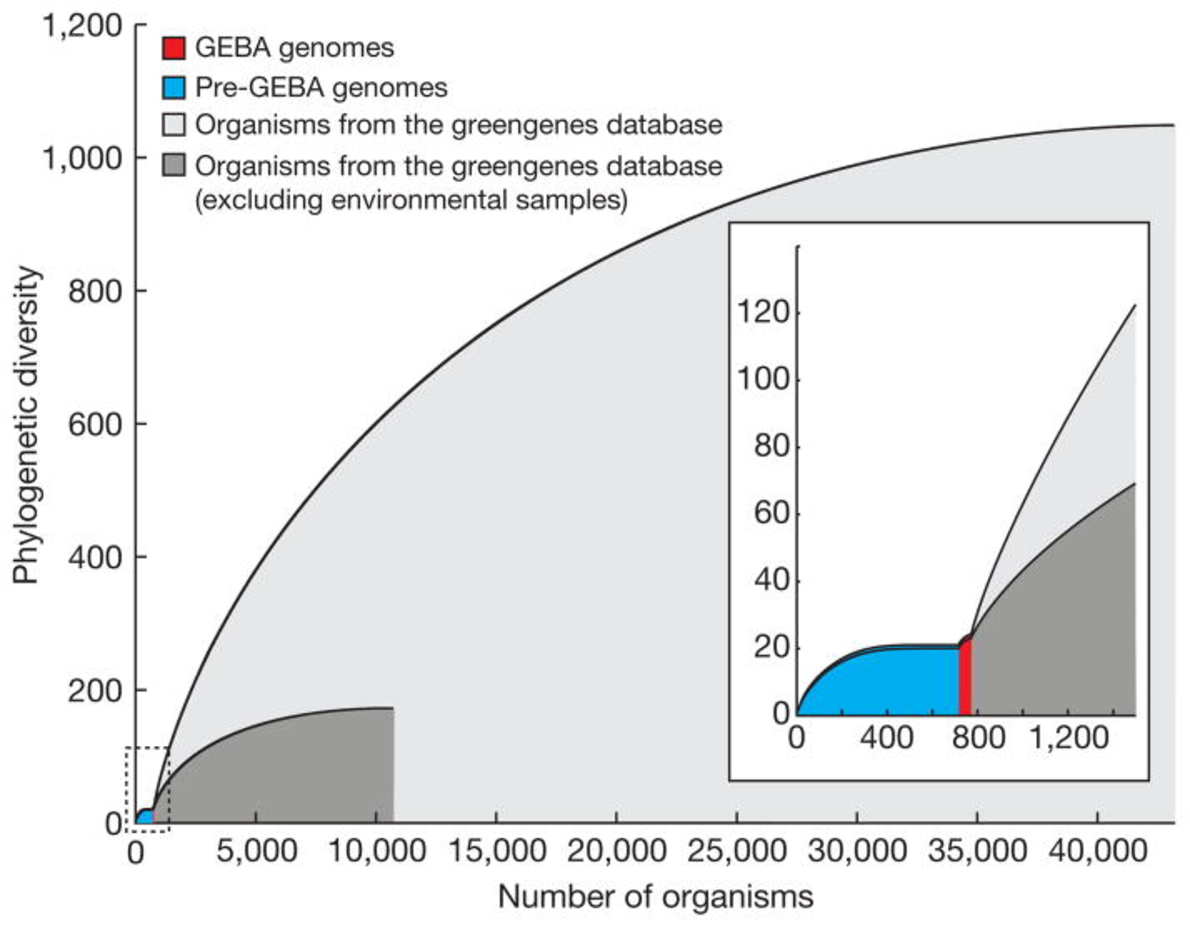
\includegraphics[width=100mm]{conc_figures/prok_diversity.pdf}
\caption[Plot of the diversity of \emph{Bacteria} and \emph{Archaea} from \citet{Wu2009}]{ Plot of the diversity of \emph{Bacteria} and \emph{Archaea} from \citet{Wu2009}. 
The diversity as shown by sequencing of 16S \acp{SSU} genes from the environment, from known organisms and from genomes is compared.
The inset shows the diversity encompassed from sequenced genomes before and after the Genomic Encyclopedia of \emph{Bacteria} and \emph{Archaea} (GEBA) sequencing project, which targets genomes for sequencing based on phylogenetic diverisity \cite{Wu2009}.
}
\label{fig:prok_diversity}

\end{figure}


\section{Concluding remarks}

This thesis has demonstrated how metagenomics and metaproteomics can be used as a tool for characterising Antarctic lake ecosystems.
The \textsc{DNA} sequence and mass spectra data that has been produced form a lasting record of the state of the microbial communities at the point in time that they were collected.
It thus acts as a resource against which other datasets can be compared to gain an understanding variability between ecosystems and as a bench mark to gauge changes overtime.
%The data can also be specifically mined to recover features of interest, for example sequences that encode enzymes with desired activities or bioactive compounds can be recovered by synthesis from the sequence information.
As sequence databases grow and more of the microbial world is characterised, this archive of molecular data can be re-analysed to learn even more from these unique ecosystems.


%Endmainmatter-------------------------------------------------------------------------------------
\bibliographystyle{plain}
\bibliography{thesis}
\chapter{Appendices}
\label{ch:appen}

\begingroup
\footnotesize
\begin{longtable}{p{1.5cm}p{6cm}p{6cm}}
\caption[Peptide data for Organic Lake metaproteomics analysis]{Peptide data for Organic Lake metaproteomic analysis. $^a$Proteins that have some shared peptides; $^b$162322406 and 162276024 are protein homologues; $^c$A group of proteins containing similar peptides that could not be differentiated by the mass spectral analysis. Only one gene number of that groups is displayed.}
\label{tab:peptides}
\\
\toprule
\textbf{Gene ID} & \multicolumn{2}{l}{\textbf{Peptide sequences}} \\
\midrule
\endfirsthead
\multicolumn{3}{c}
{\tablename\ \thetable\ -- \textit{Continued from previous page}} \\
\toprule
\textbf{Gene ID} & \multicolumn{2}{l}{\textbf{Peptide sequences}} \\
\midrule
\endhead
\bottomrule \multicolumn{3}{r} {\textit{Continued on next page}} \\
\endfoot
\bottomrule
\endlastfoot
162322530$^a$ & R.AIDECLWAVSSLSPSSSADVK.V & R.LNFNHPCK.E \\
  & K.ALGAQPFNYTDAVDALPNSIK.A &  K.LQLNGQDR.F \\
  & R.EGTYFDQVQPFQHHTR.Y & R.NGDLAYR.T \\
  & R.HSNFAMESIEQTFNGQADFGR.R & R.NYNVLR.I \\
  & K.HYGDWMQIWCQLTLDK.N & R.QVCAPR.N \\
  & R.IDNATLQLVLSNATVEGTNTAK.V & R.RVNCTISR.N \\
  & K.INLDLR.A & R.VNCTISR.N \\
162322348 & K.GNVDVYQENK.L & K.IESDAEPSWVR.G \\
162322406$^b$ & R.QNQSCGGVNQVNGTHVNR.T  & K.TNDGTLVGK.S\\
  & R.TAFHLGDGLSR.Q & K.YVSESSTYTR.F \\
162313481 & K.ITTIPENIGQLVK.I & R.SNLQGVTEEQLMSNK.I \\
162276060 & K.TPTGLEFSLTGR.A  & R.VNHTDACSTGNK.E \\
162300260 & R.VDIEGGTPFFLK.E & K.YTFQPSELSNTYFSK.E \\
162276024$^b$ & K.LGGGISSR.S & R.TSLHMGDVLSR.K \\
  & R.SEVGFQSTMVGSDVAMQR.K & \\
162275992 & K.NINLLSAGANYGINTVGSSLR.N  & R.NPNLQIR.S \\
162300108 & K.NDNIITLLDTK.Q & K.YENGSWNTLGQLIR.G \\
  & K.NVVINSEGTIISAVNNK.G & R.LTVNNSIISK.E \\
  & K.QDVITDQTNLNVGR.L & \\
162319393$^a$ & R.AIDECLWAVNTLSPDSSSDVK.V & K.LQLNGQDR.F \\
  & K.ALGAQPFNYTDAIDALPNSVK.A & R.NGDLAYR.T \\
  & R.EGTYFDQVQPFQHHTR.S & R.NYNVLR.I \\
  & R.IDNATLQLVLSNATVEGTNTAK.V & R.QVCAPR.N \\
  & R.IMSGMGGLAYSN & R.RVNCTISR.N \\
  & K.INLDLR.A  & R.VNCTISR.N \\
  & R.LNFNHPCK.E \\
162300134$^c$ & K.ATAGDTHLGGEDFDNR.M & R.VEIIANDQGNR.T \\
  & R.IINEPTAAAIAYGLDK.K & \\
162286324$^c$ & K.DVPLVANFSAK.F & K.MKLENTVEK.M \\
OLV9 & K.AGLLSEMDAYSLYQMSR.R & R.NGSQQTWNEFR.G\\
  & K.ELVLSFSSGVK.F & K.NILPYDEFVAYK.T\\
  & K.FGTQASTLFLK.D & F.NVNVPSENTLVDR.N\\
  & R.GSSATMSGLLTK.S & K.SEVLEAK.E \\
  & K.GVASAVESAIGGAK.T & K.VSVQSADILNVITK.Q \\
  & K.HIQTTPSMVDK.Y & R.YISLHPSQYAK.L \\
  & R.ITSDVQVAVK.D  & K.YTSLGSIIVIDPVR.D \\
  & K.IYLVVRPQYR.S & \\
OLV8 & K.AGTPIPGVIYEPSYPR.W & K.TLPVFIPTIK.Y \\
  & K.DIGTDMPYFIFDK.D & K.TNGTTPPR.F \\
  & K.GGYADYR.S & K.YSEDDTNESIR.N \\
  & K.TLLEFGQSK.D & K.QAFIGLQK.T \\
\end{longtable}
\endgroup

\begin{landscape}
\begingroup
\footnotesize
\begin{longtable}{p{3cm}p{3cm}p{2cm}p{3cm}p{3cm}p{6cm}p{2cm}}
\caption[PCR-based studies of Antarctic Lakes]{Studies of Antarctic Lakes that have made use of PCR amplification and sequencing of marker genes.
}
\label{tab:pcr_lakes}
\\
\toprule
\textbf{Site} & \textbf{Environment} & \textbf{Techniques} & \textbf{Organisms} & \textbf{Key processes} & \textbf{Notes} & \textbf{Reference}\\
\midrule
\endfirsthead
\multicolumn{7}{c}
{\tablename\ \thetable\ -- \textit{Continued from previous page}} \\
\toprule
\textbf{Site} & \textbf{Environment} & \textbf{Techniques} & \textbf{Organisms} & \textbf{Key processes} & \textbf{Notes} & \textbf{Reference}\\
\midrule
\endhead
\bottomrule \multicolumn{7}{r} {\textit{Continued on next page}} \\
\endfoot
\bottomrule
\endlastfoot
Lakes Bonney, Hoare, Fryxell, Joyce, Miers and Vanda, McMurdo Dry Valleys & Fresh to hypersaline, permanently ice-covered & 16S and \emph{amoA} libraries & \emph{Betaproteobacteria}, \emph{Gammaproteobacteria} & Ammonia oxidation & Nitrifying bacterial \emph{amoA} detected in all lakes.
In meromictic lakes, the population of \emph{Beta}– and  \emph{Gammaproteobacteria} vertically stratified. 
Majority of nitrifying bacteria were \emph{Betaproteobacteria}.
 & \cite{Voytek1999}  \\
 &  &  &  &  &  &   \\
 &  &  &  &  &  &   \\
 &  &  &  &  &  &   \\
\end{longtable}
\endgroup
\end{landscape}

\begin{landscape}
\begingroup
\footnotesize
\begin{longtable}{p{1.6cm}p{1.2cm}p{1.5cm}p{1.5cm}p{2.8cm}p{13.5cm}}
\caption[Proteins identitfied in the Ace Lake 5 m sample 0.1 \textmu{}m size-fraction proteome]{Proteins identitfied in the Ace Lake 5 m sample 0.1 \textmu{}m size-fraction proteome.
(*) Protein group identification: proteins that contain similar peptides that could not be differentiated by the mass spectral analysis were grouped. Only one gene number of that group is displayed.
($a$--$z$, $aa$--$pp$) Protein ambiguity groups: proteins that have some shared peptides with one or more other proteins from the same sample depth are marked with the same letters.
}
\label{tab:ace_protids_5m_cog}
\\
\toprule
\multicolumn{6}{c}{\textbf{ 5 m - COG annotated proteins }} \\
\textbf{Gene ID} & \textbf{NSA} & \textbf{COG ID} & \textbf{KO ID} & \textbf{KEGG locus} & \textbf{COG description:KEGG description} \\
\midrule
\endfirsthead
\multicolumn{6}{c}
{\tablename\ \thetable\ -- \textit{Continued from previous page}} \\
\toprule
\textbf{Gene ID} & \textbf{NSA} & \textbf{COG ID} & \textbf{KO ID} & \textbf{KEGG locus} & \textbf{COG description:KEGG description} \\
\midrule
\endhead
\bottomrule \multicolumn{6}{r} {\textit{Continued on next page}} \\
\endfoot
\bottomrule
\endlastfoot
167852195$f$&0.02530&COG1653&K10232&AAur\_0459&sugar-binding periplasmic proteins/domains : putative alpha-glucosides-binding ABC transporter (AglE) \\
167782381*&0.01724&COG1879&K02058&Ping\_2790&periplasmic sugar-binding proteins : bifunctional carbohydrate binding and transport protein \\
167813321&0.01388&COG1629&&GFO\_2756&outer membrane receptor proteins, mostly Fe transport : TonB-dependent outer membrane receptor \\
167754347&0.01044&COG1879&K02058&CMM\_0792&periplasmic sugar-binding proteins : putative sugar ABC transporter, solute-binding protein \\
167701754$a$&0.00967&COG0834&K09969&SAR11\_0953&ABC-type amino acid transport system, periplasmic component : yhdW \\
167792775&0.00630&COG1879&K10552&SMc02171&periplasmic sugar-binding proteins : fructose transport system substrate-binding protein \\
167932252$d$&0.00537&COG0715&K02051&SAR11\_0807&ABC-type nitrate/sulfonate/taurine/bicarbonate transport systems, periplasmic components \\
167759671&0.00493&COG0605&&NEMVE\_v1g231554&superoxide dismutase \\
167751919$h$&0.00468&COG3740&&ROP\_69760&phage head maturation protease \\
167907426&0.00438&COG1638&&SAR11\_0266&dicarboxylate-binding periplasmic protein : TRAP dicarboxylate transporter - DctP subunit (mannitol/chloroaromatic compounds) \\
167711086&0.00425&COG0834&K02030&TM1040\_0294&ABC-type amino acid transport system, periplasmic component : lysine-arginine-ornithine-binding periplasmic protein \\
167819184&0.00389&COG2113&K02002&SAR11\_1302&ABC-type proline/glycine betaine transport systems, periplasmic components : opuAC \\
167680030&0.00346&COG0683&K01999&AAur\_1271&ABC-type branched-chain amino acid transport systems, periplasmic component : braC \\
167865828$b$&0.00338&COG0834&K09969&HCH\_05807&ABC-type amino acid transport system, periplasmic component \\
167684228$c$&0.00331&COG0459&K04077&SAR11\_0162&chaperonin GroEL (HSP60 family) \\
167868594$d$&0.00311&COG0715&K02051&SAR11\_0807&ABC-type nitrate/sulfonate/taurine/bicarbonate transport systems, periplasmic components \\
167785199$c$&0.00309&COG0459&K04077&CHU\_1828&chaperonin GroEL (HSP60 family) \\
167819050&0.00304&COG2113&K02001&Plav\_1066&ABC-type proline/glycine betaine transport systems, periplasmic components \\
167867034&0.00284&COG0687&K02055&SAR11\_1336&spermidine/putrescine-binding periplasmic proteinp : potD; \\
167700934&0.00277&COG0450&&SPO3383&peroxiredoxin : thiol-specific antioxidant protein \\
167816084$a$&0.00253&COG0834&K09969&SAR11\_0953&ABC-type amino acid transport system, periplasmic component : yhdW \\
167714114&0.00179&COG0687&K02055&SAR11\_1336&spermidine/putrescine-binding periplasmic protein : potD \\
167712994$b$&0.00175&COG0834&K09969&HCH\_05807&ABC-type amino acid transport system, periplasmic component \\
167824568&0.00164&COG3181&&Dshi\_2450&uncharacterized BCR : hypothetical protein \\
167925495&0.00159&COG1653&K02027&Krad\_1380&sugar-binding periplasmic proteins/domains \\
167695410$a$&0.00155&COG0834&K09969&SAR11\_0953&ABC-type amino acid transport system, periplasmic component : yhdW \\
167695984*&0.00138&COG1879&&&periplasmic sugar-binding proteins \\
167703404&0.00134&COG1012&K00128&AAur\_pTC20196&NAD-dependent aldehyde dehydrogenases \\
167718230&0.00125&COG0683&K01999&AAur\_1271&ABC-type branched-chain amino acid transport systems, periplasmic component : braC \\
167735996&0.00103&COG0591&&SAR11\_0316&Na$+$/proline, Na$+$/panthothenate symporters and related permeases : yjcG \\
167739054&0.00101&COG1028&K00059&SH0230&dehydrogenases with different specificities (related to short-chain alcohol dehydrogenases) : 3-oxoacyl-[acyl-carrier protein] reductase \\
167701096&0.00100&COG0776&&KRH\_03630&bacterial nucleoid DNA-binding protein : HU\_IHF family transcriptional regulator \\
167817334&0.00098&COG0715&&FRAAL1422&ABC-type nitrate/sulfonate/taurine/bicarbonate transport systems, periplasmic components \\
167703266$c$&0.00095&COG0459&K04077&Noca\_3982&chaperonin GroEL (HSP60 family) \\
167768609&0.00095&COG3181&&RD1\_2202&uncharacterized BCR \\
167868532&0.00093&COG3181&K07795&HCH\_01639&uncharacterized BCR : putative tricarboxylic transport membrane protein \\
167865516&0.00088&COG0747&&CMM\_2185&ABC-type dipeptide/oligopeptide/nickel transport systems, periplasmic components \\
167911715&0.00083&COG0776&K03530&Sala\_0799&bacterial nucleoid DNA-binding protein : DNA-binding protein HU-beta \\
167736316&0.00082&COG0174&K01915&SAR11\_0747&glutamine synthase : glnA \\
167916441&0.00079&COG1629&&BF2044&outer membrane receptor proteins, mostly Fe transport : putative TonB-dependent outer membrane receptor protein \\
167920571&0.00078&COG0776&K03530&SAR11\_0817&bacterial nucleoid DNA-binding protein : hupA \\
167703332&0.00066&COG1732&K05845&Strop\_1633&periplasmic glycine betaine/choline-binding (lipo)protein of an ABC-type transport system (osmoprotectant binding protein) \\
167662373&0.00063&COG0834&&Pden\_1025&ABC-type amino acid transport system, periplasmic component : extracellular solute-binding protein, family 3 \\
167890974&0.00062&COG1878&&nfa12380&uncharacterized ACR, predicted metal-dependent hydrolases \\
167824660&0.00061&COG0683&K01999&SAR11\_1361&ABC-type branched-chain amino acid transport systems, periplasmic component : livJ2; Leu/Ile/Val-binding protein precursor \\
167886240&0.00061&COG0335&K02884&CHU\_0120&rplS; 50S ribosomal protein L19 \\
167921445&0.00058&COG0811&&GFO\_0088&biopolymer transport proteins : exbB; ExbB-like MotA/TolQ/ExbB family \\
167776275$ee$&0.00055&COG3740&K06904&BL0376&phage head maturation protease \\
167659892*$ee$&0.00055&COG3740&&ROP\_69760&phage head maturation protease \\
167786475&0.00054&COG0098&K02988&Fjoh\_0380&rpsE; 30S ribosomal protein S5 \\
167693676*&0.00054&COG0776&&Arth\_3916&bacterial nucleoid DNA-binding protein \\
167818330&0.00048&COG0683&&Rxyl\_0363&ABC-type branched-chain amino acid transport systems, periplasmic component : extracellular ligand-binding receptor \\
167739596&0.00044&COG0545&K03772&BDI\_2705&FKBP-type peptidyl-prolyl cis-trans isomerases 1 \\
167808311$c$&0.00044&COG0459&K04077&SAR11\_0162&chaperonin GroEL (HSP60 family) \\
167706214&0.00044&COG0683&&Tfu\_1779&ABC-type branched-chain amino acid transport systems, periplasmic component \\
167866918&0.00044&COG2885&K03640&SAR11\_0598&outer membrane protein and related peptidoglycan-associated (lipo)proteins : ompA; OmpA family \\
167807477&0.00042&COG0834&&MSMEG\_5368&ABC-type amino acid transport system, periplasmic component : ehuB; ectoine/hydroxyectoine ABC  transporter solute-binding protein \\
167881416$e$&0.00040&COG0050&K02358&CHU\_3175&GTPases - translation elongation factors : tufB, tuf \\
167765645$f$&0.00034&COG1653&K10232&Sare\_3967&sugar-binding periplasmic proteins/domains \\
167730910&0.00033&COG3181&&Dshi\_2450&uncharacterized BCR \\
167725574&0.00032&COG0450&K03386&CHU\_2724&peroxiredoxin : ahpC; alkyl hydroperoxide reductase, subunit C \\
167768817&0.00032&COG0740&K00288&CHU\_1706&protease subunit of ATP-dependent Clp proteases : methylenetetrahydrofolate dehydrogenase (NADP$+$) \\
167886236&0.00031&COG0228&K02959&CHU\_0117&rpsP; 30S ribosomal protein S16 \\
167907528&0.00031&COG0591&&SAR11\_0316&Na$+$/proline, Na$+$/panthothenate symporters and related permeases : yjcG \\
167868396&0.00029&COG2358&&PBPRA0389&predicted periplasmic binding protein : putative immunogenic protein \\
167718328&0.00027&COG1744&K07335&AAur\_1253&surface lipoprotein : basic membrane protein A and related proteins \\
167769503$c$&0.00027&COG0459&&CMS\_2756&chaperonin GroEL (HSP60 family) \\
167818958&0.00026&COG1638&&TM1040\_0356&dicarboxylate-binding periplasmic protein : TRAP dicarboxylate transporter - DctP subunit \\
167702878&0.00025&COG1879&&Krad\_1186&periplasmic sugar-binding proteins : periplasmic binding protein/LacI transcriptional regulator \\
167665756&0.00025&COG0091&K02890&GFO\_2834&rplV; 50S ribosomal protein L22 \\
167730894&0.00023&COG1638&&RD1\_2185&dicarboxylate-binding periplasmic protein : dctP; C4-dicarboxylate-binding periplasmic protein, putative \\
167680092&0.00022&COG0094&K02931&Lxx20210&rplE; 50S ribosomal protein L5 \\
167868548&0.00020&COG0834&K10018&SAR11\_1210&ABC-type amino acid transport system, periplasmic component : octopine/nopaline transport system substrate-binding protein \\
167892279&0.00019&COG0834&K02030&Veis\_2153&ABC-type amino acid transport system, periplasmic component \\
167817276&0.00018&COG0347&K04751&Acel\_1565&nitrogen regulatory protein PII \\
167862242&0.00018&COG0087&K02906&BT\_2727&rplC; 50S ribosomal protein L3 \\
167933288&0.00018&COG1638&&Dshi\_3326&dicarboxylate-binding periplasmic protein : TRAP dicarboxylate transporter-DctP subunit \\
167713980*&0.00016&COG0330&K04088&SAR11\_0008&membrane protease subunits, stomatin/prohibitin homologs : hflK \\
167867886&0.00016&COG3181&&Csal\_1767&uncharacterized BCR : uncharacterized protein UPF0065 \\
167809873&0.00016&COG0539&K02945&CHU\_1951&rpsA; 30S ribosomal protein S1 \\
167713982&0.00015&COG0330&K04087&SAR11\_0007&membrane protease subunits, stomatin/prohibitin homologs : hflC \\
167822210&0.00015&COG0776&&SCO2950&bacterial nucleoid DNA-binding protein : hup, SCE59.09c; DNA-binding protein Hu (hs1) \\
167820450*&0.00015&COG1192&&tlr0963&ATPases involved in chromosome partitioning : probable cell division inhibitor minD \\
167820614$g$&0.00015&COG0174&K01915&Krad\_3291&glutamine synthase \\
167714092&0.00014&COG0683&K01999&SAR11\_1346&ABC-type branched-chain amino acid transport systems, periplasmic component : livJ \\
167817130&0.00014&COG0711&K02109&SCO5369&F0F1-type ATP synthase b subunit \\
167818902&0.00014&COG1638&&SAR11\_0864&dicarboxylate-binding periplasmic protein \\
167866078&0.00013&COG0605&K00518&Arth\_2086&superoxide dismutase \\
167865698&0.00013&COG0740&K01358&AAur\_2381&protease subunit of ATP-dependent Clp proteases \\
167817852&0.00013&COG0683&&Noca\_3017&ABC-type branched-chain amino acid transport systems, periplasmic component : extracellular ligand -binding receptor \\
167714042&0.00012&COG0683&K01999&SAR11\_1361&ABC-type branched-chain amino acid transport systems, periplasmic component : livJ2; Leu/Ile/Val-binding protein precursor \\
167821000&0.00012&COG1732&&MSMEG\_2924&periplasmic glycine betaine/choline-binding (lipo)protein of an ABC-type transport system (osmoprotectant binding protein) : permease binding-protein component \\
167668848$g$&0.00011&COG0174&K01915&CMM\_1636&glutamine synthase : glnA1 \\
167748683*&0.00010&COG0834&&PFL\_3548&ABC-type amino acid transport system, periplasmic component \\
167718146&0.00010&COG0088&K02926&Lxx20320&rplD; 50S ribosomal protein L4 \\
167862420&0.00010&COG1629&&FP0112&outer membrane receptor proteins, mostly Fe transport : probable TonB-dependent outer membrane receptor precursor \\
167696080*&0.00010&COG1344&K02406&Csac\_1680&flagellin and related hook-associated proteins \\
167735512&0.00010&COG0803&K09815&Smed\_1697&ABC-type Mn/Zn transport system, periplasmic Mn/Zn-binding (lipo)protein (surface adhesin A) \\
167719882&0.00009&COG0096&K02994&SAR11\_1103&rpsH; 30S ribosomal protein S8 \\
167660431$h$&0.00009&COG3740&K06904&BL0376&phage head maturation protease \\
167718250&0.00009&COG2213&K02799&GK1948&phosphotransferase system, mannitol-specific IIBC component \\
167719862*&0.00008&COG0185&K02965&SAR11\_1113&rpsS; 30S ribosomal protein S19 \\
167702806&0.00008&COG0081&K02863&KRH\_05860&rplA; 50S ribosomal protein L1 \\
167719824*$e$&0.00008&COG0050&K02358&SAR11\_1130&GTPases - translation elongation factors : tufB, tuf \\
167817466&0.00008&COG0404&&mll1258&glycine cleavage system T protein (aminomethyltransferase) : sarcosine dehydrogenase \\
167868614&0.00008&COG2113&K02002&SAR11\_0797&ABC-type proline/glycine betaine transport systems, periplasmic components : proX \\
167933120&0.00007&COG0803&K09815&Atu1521&ABC-type Mn/Zn transport system, periplasmic Mn/Zn-binding (lipo)protein (surface adhesin A) : znuA \\
167718168&0.00007&COG0094&&CMS\_0295&50S ribosomal protein L5 \\
167868724&0.00007&COG0396&K09013&SAR11\_0740&iron-regulated ABC transporter ATPase subunit SufC \\
167718156&0.00007&COG0092&K02982&Krad\_0694&ribosomal protein S3 \\
167719956&0.00006&COG0834&K02030&SAR11\_1068&ABC-type amino acid transport system, periplasmic component : pheC; cyclohexadienyl dehydratase \\
167730882&0.00006&COG0004&&SAR11\_0818&ammonia permeases : amtB; ammonium transporter \\
167718138e&0.00006&COG0050&K02358&Tfu\_2648&GTPases - translation elongation factors: tuf \\
167718052&0.00006&COG1653&K02027&Krad\_3469&sugar-binding periplasmic proteins/domains \\
167700960*&0.00006&COG3794&&SMa1243&plastocyanin :  Azu1 pseudoazurin (blue copper protein) \\
167868482&0.00005&COG0715&&&ABC-type nitrate/sulfonate/taurine/bicarbonate transport systems, periplasmic components \\
167868656&0.00005&COG0715&K02051&AZC\_2351&ABC-type nitrate/sulfonate/taurine/bicarbonate transport systems, periplasmic components \\
167868494&0.00004&COG1638&&SMa0157&dicarboxylate-binding periplasmic protein \\
167866460&0.00004&COG0687&K02055&SCO5667&spermidine/putrescine-binding periplasmic protein \\
167719840&0.00004&COG0085&K03043&SAR11\_1123&DNA-directed RNA polymerase beta subunit/140 kD subunit (split gene in Mjan, Mthe, Aful) : rpoB \\
167816636&0.00004&COG0459&K04077&Krad\_0736&chaperonin GroEL (HSP60 family) \\
167701680*&0.00004&COG3740&K06904&BL0376&phage head maturation protease \\
167717794*&0.00003&COG0195&K02600&SAR11\_0388&phage head maturation protease \\
167717838&0.00003&COG0443&K04043&SAR11\_0368&molecular chaperone : dnaK \\
167834314&0.00003&COG0443&&CMS\_2806&molecular chaperone : dnaK \\
167717784&0.00003&COG1185&K00962&SAR11\_0392&polyribonucleotide nucleotidyltransferase (polynucleotide phosphorylase) \\
167818278&0.00003&COG1022&&Noca\_3113&long-chain acyl-CoA synthetases (AMP-forming) : AMP-dependent synthetase and ligase \\
167719850&0.00002&COG0480&K02355&SAR11\_1119&translation elongation and release factors (GTPases) : fusA \\
167816480&0.00002&COG0086&K03046&Krad\_0681&DNA-directed RNA polymerase beta' subunit/160 kD subunit (split gene in archaea and Syn) \\
167866408&0.00001&COG1185&K00962&Lxx09030&polyribonucleotide nucleotidyltransferase (polynucleotide phosphorylase) \\
\multicolumn{6}{c}{\textbf{ 5 m - KEGG and NR annotated proteins}} \\
\textbf{Gene ID} & \textbf{NSA} & \textbf{NR ID} & \textbf{KO ID} & \textbf{KEGG/NR Locus} & \textbf{KEGG/NR description} \\
167873078&0.03710&BAF91544&&&major capsid protein [uncultured Myoviridae] \\
167771989$i$&0.02658&&&BTH\_I0914&hypothetical protein \\
167723550$j$&0.01559&YP\_001648266&&OsV5\_190f&hypothetical protein [Ostreococcus virus OsV5] \\
167927818$j$&0.01345&YP\_001648266&&OsV5\_190f&hypothetical protein [Ostreococcus virus OsV5] \\
167933090&0.01298&YP\_002590925&&&putative porin [Candidatus Pelagibacter sp. HTCC7211] \\
167711088&0.01230&&K09969&PBPRA2185&putative amino acid ABC transporter, periplasmic amino acid-binding protein \\
167691398&0.01175&&&HM1\_2880&phage major capsid protein, hk97 family \\
167922719$k$&0.01174&&&Neut\_1469&phage major capsid protein, HK97 family protein \\
167775105$l$&0.01103&ABC95191&&&GP23-major capsid protein [Stenotrophomonas phage SMB14] \\
167687982$l$&0.00968&NP\_944113&&&gp23 major head protein [Aeromonas phage Aeh1] \\
167748599$m$&0.00960&&&M6\_Spy1138&phage prohead protease \\
167733772&0.00952&&&BBta\_5785&putative phage major head protein \\
167925660&0.00923&&&SRU\_2178&putative outer membrane protein, probably involved in nutrient binding \\
167796059$n$&0.00853&&&APECO1\_525&hypothetical protein \\
167883590&0.00820&&&PP\_1567&phage major capsid protein, HK97 family \\
167666520$o$&0.00818&BAF91544&&&major capsid protein [uncultured Myoviridae] \\
167664173*$p$&0.00713&&&GDI3673&hypothetical protein \\
167667150$m$&0.00687&&&LGAS\_1485&predicted phage phi-C31 GP36 major capsid-like protein \\
167771337&0.00605&ABW90951&&&gp23 major capsid protein [uncultured Myoviridae] \\
167884290$l$&0.00573&BAF91544&&&major capsid protein [uncultured Myoviridae] \\
167760139&0.00561&&&CHU\_2679&probable outer membrane lipoprotein P61 \\
167816468$q$&0.00522&&&DR\_A0099&hypothetical protein \\
167700634$j$&0.00499&YP\_001648266&&OsV5\_190f&hypothetical protein [Ostreococcus virus OsV5] \\
167687792$r$&0.00498&&&Asuc\_1240&phage major capsid protein, HK97 family \\
167842580$r$&0.00453&&&BAV1464&major capsid protein \\
167700776&0.00447&&&Bpro\_3745&hypothetical protein \\
167729766&0.00433&ZP\_01224596&&GB2207\_03424&hypothetical protein [marine gamma proteobacterium HTCC2207] \\
167934698&0.00431&&&Swit\_4452&hypothetical protein \\
167884738&0.00409&&&BBta\_5785&putative phage major head protein \\
167669610$p$&0.00397&&&GDI3673&hypothetical protein \\
167861688&0.00359&&&BDI\_2874&putative outer membrane protein, probably involved in nutrient binding \\
167910063&0.00347&&&GDI3673&hypothetical protein \\
167893743*$s$&0.00338&YP\_001648158&&OsV5\_081f&hypothetical protein [Ostreococcus virus OsV5] \\
167888926$p$&0.00326&&&GDI3673&hypothetical protein \\
167753643*&0.00324&&&Daci\_1946&putative phage major head protein \\
167742624$p$&0.00317&&&GDI3673&hypothetical protein \\
167908539$r$&0.00304&&&BAV1464&major capsid protein \\
167675286*&0.00284&&&CKO\_01864&hypothetical protein \\
167900893$n$&0.00278&&&APECO1\_525&hypothetical protein \\
167778265$p$&0.00275&&&GDI3673&hypothetical protein \\
167786471&0.00267&&&mlr8524&phage major capsid protein, GP36 \\
167735768&0.00265&&&FRAAL2681&hypothetical protein \\
167773951$t$&0.00253&&&LGAS\_1485&predicted phage phi-C31 GP36 major capsid-like protein \\
167841586$j$&0.00250&A7U6E7&&&putative major capsid protein [Chrysochromulina ericina virus] \\
167919545&0.00245&&&Pmen\_3970&phage major capsid protein, HK97 family \\
167781901$u$&0.00236&YP\_214367&&&T4-like major capsid protein [Prochlorococcus phage P-SSM2] \\
167923659$p$&0.00235&&&GDI3673&hypothetical protein \\
167852301$v$&0.00230&&&MAB\_1788&bacteriophage protein \\
167659301&0.00224&&&LGAS\_1485&predicted phage phi-C31 GP36 major capsid-like protein \\
167861686&0.00223&YP\_002789013&&&TonB dependent/ligand-gated channel [Polaribacter sp. MED152] \\
167712528$v$&0.00215&&&MAB\_1788&bacterial nucleoid DNA-binding protein \\
167678920*$w$&0.00209&YP\_001498525&&AR158\_C444L&hypothetical protein [Paramecium bursaria Chlorella virus AR158] \\
167849540$j$&0.00201&YP\_001648266&&OsV5\_190f&hypothetical protein [Ostreococcus virus OsV5] \\
167781903$u$&0.00201&YP\_214367&&&T4-like major capsid protein [Prochlorococcus phage P-SSM2] \\
167863158$j$&0.00200&YP\_001648266&&OsV5\_190f&hypothetical protein [Ostreococcus virus OsV5] \\
167663967*&0.00190&&&Swit\_4461&hypothetical protein \\
167687108$u$&0.00182&YP\_214367&&&T4-like major capsid protein [Prochlorococcus phage P-SSM2] \\
167692622$i$&0.00176&&&SG1188&hypothetical protein \\
167733858&0.00170&ZP\_01017474&&&major capsid protein, HK97 family protein [Parvularcula bermudensis HTCC2503] \\
167852851$p$&0.00167&&&GDI3673&hypothetical protein \\
167864542$k$&0.00166&&&Neut\_1469&phage major capsid protein, HK97 family protein \\
167803157&0.00165&ZP\_01688540&&&lipoprotein, putative [Microscilla marina ATCC 23134] \\
&&&&& \\
167682644$j$&0.00153&A7U6E7&&&putative major capsid protein [Chrysochromulina ericina virus] \\
167733004*$j$&0.00150&A7U6F0&&&putative major capsid protein [Phaeocystis pouchetii virus] \\
167765429&0.00148&&&CHU\_2610&gliding motility-related protein; possible GldN and/or GldO \\
167878228$t$&0.00145&&&LGAS\_1485&predicted phage phi-C31 GP36 major capsid-like protein \\
167775103&0.00145&YP\_214669&&&gp23 [Prochlorococcus phage P-SSM4] \\
167702908&0.00143&&&mma\_2202&hypothetical protein \\
167869946&0.00135&YP\_195142&&&major capsid protein gp23 [Synechococcus phage S-PM2] \\
167834518&0.00128&&&Haur\_0657&hypothetical protein \\
167807747&0.00122&&&Saro\_0657&hypothetical protein \\
167816420&0.00121&&&APECO1\_525&hypothetical protein \\
167809283$k$&0.00119&&&Neut\_1469&phage major capsid protein, HK97 family protein \\
167868514&0.00119&&&SAR11\_1290&TRAP-type bacterial extracellular solute-binding protein \\
167750765&0.00118&&&Smed\_1334&phage major capsid protein, HK97 family \\
167925457$p$&0.00115&&&GDI3673&hypothetical protein \\
167782759&0.00113&&&Oter\_1957&band 7 protein \\
167871794$j$&0.00113&YP\_001648266&&OsV5\_190f&hypothetical protein [Ostreococcus virus OsV5] \\
167756019&0.00112&&&CHU\_0172&gldL; gliding motility-related protein \\
167670926$x$&0.00112&&&BBta\_5785&putative phage major head protein \\
167821362$z$&0.00112&&&APECO1\_525&hypothetical protein \\
167690910$j$&0.00111&YP\_001648266&&OsV5\_190f&hypothetical protein [Ostreococcus virus OsV5] \\
167685332$j$&0.00110&YP\_001648266&&OsV5\_190f&hypothetical protein [Ostreococcus virus OsV5] \\
167700460*&0.00110&YP\_001648158&&OsV5\_081f&hypothetical protein [Ostreococcus virus OsV5] \\
167685474*$aa$&0.00104&YP\_001648182&&OsV5\_105r&hypothetical protein [Ostreococcus virus OsV5] \\
167734326$bb$&0.00103&&&amb4267&hypothetical protein \\
16775653$q$&0.00101&&&Haur\_0657&hypothetical protein \\
167733302$p$&0.00101&&&GDI3673&hypothetical protein \\
167663981$p$&0.00097&&&GDI3673&hypothetical protein \\
167763843&0.00096&&&Saro\_0657&hypothetical protein \\
167768193$z$&0.00096&&&CKO\_01864&hypothetical protein \\
167719228$i$&0.00095&&&SG1188&hypothetical protein \\
167844676&0.00091&ZP\_03643684&&BACCOPRO\_02057&hypothetical protein [Bacteroides coprophilus DSM 18228] \\
167881504$cc$&0.00091&&&BSU26140&yqbE; hypothetical protein \\
167852559$oo$&0.00090&&&HSM\_0907&hypothetical protein \\
167804465*&0.00088&ZP\_03724502&&ObacDRAFT\_9001&hypothetical protein [Opitutaceae bacterium TAV2] \\
167794165$p$&0.00087&&&GDI3673&hypothetical protein \\
167734676&0.00085&&&Amet\_4028&phage major capsid protein, HK97 family \\
167764813$u$&0.00084&YP\_214367&&&T4-like major capsid protein [Prochlorococcus phage P-SSM2] \\
167781783$p$&0.00079&&&GDI3673&hypothetical protein \\
167759955&0.00077&&&Dgeo\_0628&hypothetical protein \\
167733674&0.00076&&&Swit\_4452&hypothetical protein \\
167878828&0.00075&&K02027&SAV1394&ABC transporter solute-binding protein \\
167740142&0.00075&YP\_002705257&&&gp34 [Stenotrophomonas sp. SKA14] \\
167834088&0.00074&&&Haur\_0657&hypothetical protein \\
167821604$j$&0.00072&YP\_001648266&&OsV5\_190f&hypothetical protein [Ostreococcus virus OsV5] \\
167798697$p$&0.00070&&&GDI3673&hypothetical protein \\
167823322$s$&0.00070&YP\_001648158&&OsV5\_081f&hypothetical protein [Ostreococcus virus OsV5] \\
167718758$j$&0.00070&A7U6F0&&&putative major capsid protein [Phaeocystis pouchetii virus] \\
167713806&0.00069&&&SG1188&hypothetical protein \\
167778269$dd$&0.00068&YP\_002276820&&Gdia\_2460&hypothetical protein [Gluconacetobacter diazotrophicus PAl 5] \\
167879936$s$&0.00067&YP\_001648158&&OsV5\_081f&hypothetical protein [Ostreococcus virus OsV5] \\
167701850&0.00064&&&M446\_5960&hypothetical protein \\
167934792$p$&0.00064&&&GDI3673&hypothetical protein \\
167874674&0.00063&&&GFO\_0492&conserved hypothetical protein, secreted-possibly porin \\
167821292&0.00062&&&Oant\_1504&peptidase U35 phage prohead HK97 \\
167867556&0.00062&&&Rru\_A2587&hypothetical protein \\
167901481&0.00061&&&Cthe\_1719&phage major capsid protein, HK97 family \\
167824444&0.00059&&&Smed\_5134&TRAP dicarboxylate transporter-DctP subunit \\
167696166*&0.00059&&&BTH\_I0915&hypothetical protein \\
167936648&0.00056&EEI06235&&XcelDRAFT\_1815&hypothetical protein [Xylanimonas cellulosilytica DSM 15894] \\
167910361$j$&0.00054&A7U6F0&&&putative major capsid protein [Phaeocystis pouchetii virus] \\
167675492*$p$&0.00054&&&GDI3673&hypothetical protein \\
167801933$aa$&0.00052&YP\_001648182&&OsV5\_105r&hypothetical protein [Ostreococcus virus OsV5] \\
167725772$cc$&0.00051&&&BSU26140&yqbE; hypothetical protein \\
167820670&0.00050&&&gll0198&similar to bacteriorhodopsin \\
167832972$t$&0.00050&&&LGAS\_1485&predicted phage phi-C31 GP36 major capsid-like protein \\
167867536&0.00049&&&TM1040\_0812&hypothetical protein \\
167783747&0.00048&&&Glov\_2914&cell surface receptor IPT/TIG domain protein \\
167893945&0.00048&&&Oter\_3420&hypothetical protein \\
167740708&0.00047&&K03286&Pnap\_1319&OmpA/MotB domain protein; OmpA-OmpF porin, OOP family \\
167772783&0.00047&&&RCIX1696&hypothetical protein \\
167734614$p$&0.00047&&&GDI3673&hypothetical protein \\
167776587*&0.00046&YP\_001648249&&OsV5\_172f&hypothetical protein [Ostreococcus virus OsV5] \\
167911245$s$&0.00046&YP\_001648315&&OsV5\_239r&hypothetical protein [Ostreococcus virus OsV5] \\
167867748$x$&0.00044&&&Daci\_1946&putative phage major head protein \\
167732694&0.00044&&&NMC0858&putative phage-related protein \\
167922873&0.00042&&&CHU\_3230&hypothetical protein \\
167734178$p$&0.00041&&&GDI3673&hypothetical protein \\
167873260&0.00041&&&Sare\_3763&hypothetical protein \\
167685638*$w$&0.00041&YP\_001498525&&AR158\_C444L&hypothetical protein [Paramecium bursaria Chlorella virus AR158] \\
167901149&0.00040&&K01358&azo1870&endopeptidase Clp; K01358 ATP-dependent Clp protease, protease subunit \\
167853099$i$&0.00040&&&SG1188&hypothetical protein \\
167761349$x$&0.00037&&&Daci\_1946&putative phage major head protein \\
167776241&0.00037&&&mll0455&hypothetical protein \\
167824154&0.00036&&&SACE\_4894&hydrolase, alpha/beta fold family \\
167843578$s$&0.00035&YP\_001648158&&OsV5\_081f&hypothetical protein [Ostreococcus virus OsV5] \\
167682808*&0.00035&YP\_001648239&&OsV5\_162f&hypothetical protein [Ostreococcus virus OsV5] \\
167703228&0.00034&&&Dshi\_0412&beta-Ig-H3/fasciclin \\
167918033$p$&0.00034&&&GDI3673&hypothetical protein \\
167891224$p$&0.00033&&&GDI3673&hypothetical protein \\
167867622&0.00033&&&Oant\_1504&peptidase U35 phage prohead HK97 \\
167732430$ff$&0.00031&ZP\_02092868&&FAEPRAM212\_03171&hypothetical protein [Faecalibacterium prausnitzii M21/2] \\
167684500s&0.00031&YP\_001648158&&OsV5\_081f&hypothetical protein [Ostreococcus virus OsV5] \\
167824164*&0.00030&YP\_001648240&&OsV5\_163f&hypothetical protein [Ostreococcus virus OsV5] \\
167765431&0.00030&&&CHU\_0173&gldM; gliding motility-related protein \\
167854137&0.00030&ZP\_00743477&&RBTH\_08297&hypothetical protein [Bacillus thuringiensis serovar israelensis ATCC 35646] \\
167730288$k$&0.00028&&&Neut\_1469&phage major capsid protein, HK97 family protein \\
167685472*$gg$&0.00027&YP\_001648184&&OsV5\_107r&hypothetical protein [Ostreococcus virus OsV5] \\
167778267$p$&0.00027&&&GDI3673&hypothetical protein \\
167919557&0.00027&&&PputW619\_3936&hypothetical protein \\
167782645&0.00026&&&BBta\_5785&putative phage major head protein \\
167908551&0.00026&&&CC\_2781&hypothetical protein \\
16786723$p$&0.00026&&&GDI3673&hypothetical protein \\
167896531&0.00026&&&BAV1464&major capsid protein \\
167821374&0.00025&YP\_001919460&&Mpop\_5468&hypothetical protein [Methylobacterium populi BJ001] \\
167833472&0.00024&&&GDI3673&hypothetical protein \\
167733210&0.00024&&&Pmen\_3970&phage major capsid protein, HK97 family \\
167713652*&0.00023&&&mlr8533&hypothetical protein \\
167935700$p$&0.00023&&&GDI3673&hypothetical protein \\
167872214$hh$&0.00023&&K06907&Sfum\_3815&phage tail sheath protein \\
167881636&0.00023&&&Rsph17025\_0103&hypothetical protein \\
167791200$p$&0.00023&&&GDI3673&hypothetical protein \\
167922981$p$&0.00022&&&GDI3673&hypothetical protein \\
167824604&0.00022&&&Rsph17029\_3578&uncharacterized protein UPF0065 \\
167933608$ff$&0.00022&ZP\_02092868&&FAEPRAM212\_03171&hypothetical protein [Faecalibacterium prausnitzii M21/2] \\
167817058&0.00022&&K00518&Sare\_4077&superoxide dismutase \\
167823358*$gg$&0.00021&YP\_001648184&&OsV5\_107r&hypothetical protein [Ostreococcus virus OsV5] \\
167892855&0.00021&YP\_001648184&&OsV5\_107r&hypothetical protein [Ostreococcus virus OsV5] \\
167840790&0.00021&&&Rsph17025\_0437&hypothetical protein \\
167712150*$s$&0.00021&YP\_001648158&&OsV5\_081f&hypothetical protein [Ostreococcus virus OsV5] \\
167833160$bb$&0.00021&&&amb4267&hypothetical protein \\
167892985$j$&0.00021&YP\_001648266&&OsV5\_190f&hypothetical protein [Ostreococcus virus OsV5] \\
167696294$oo$&0.00020&&&HS\_1377&hypothetical protein \\
167759041&0.00019&&&PP\_3877&hypothetical protein \\
167766087$s$&0.00019&YP\_001648153&&OsV5\_076f&hypothetical protein [Ostreococcus virus OsV5] \\
167919775&0.00019&YP\_001294637&&ORF044&hypothetical protein [Pseudomonas phage PA11] \\
167804453*&0.00017&ZP\_03724505&&ObacDRAFT\_9004&hypothetical protein [Opitutaceae bacterium TAV2] \\
167833104&0.00017&&&Bcep1808\_1173&hypothetical protein \\
167721370*&0.00016&YP\_001648301&&OsV5\_225r&hypothetical protein [Ostreococcus virus OsV5] \\
167826943*&0.00016&&&Sare\_3763&hypothetical protein \\
167865492&0.00015&&K02027&Pput\_3473&extracellular solute-binding protein, family 1; multiple sugar transport system substrate-binding protein \\
167685780*$j$&0.00015&YP\_001648266&&OsV5\_190f&hypothetical protein [Ostreococcus virus OsV5] \\
167910713&0.00014&&&Bd1641&hypothetical protein \\
167910061$p$&0.00014&&&GDI3673&hypothetical protein \\
167833358$s$&0.00013&YP\_001648158&&OsV5\_081f&hypothetical protein [Ostreococcus virus OsV5] \\
167692314*$w$&0.00012&YP\_001498525&&AR158\_C444L&hypothetical protein [Paramecium bursaria Chlorella virus AR158] \\
167925393&0.00012&&&Oter\_3421&hypothetical protein \\
167687436&0.00011&&K01999&azo3443&conserved hypothetical ABC-type branched-chain amino acid transport systems, periplasmic component \\
167719658$hh$&0.00011&&K06907&Dde\_1889&hypothetical protein \\
167668360$s$&0.00011&YP\_001648158&&OsV5\_081f&hypothetical protein [Ostreococcus virus OsV5] \\
167735772&0.00010&&&FRAAL2683&hypothetical protein; putative mycobacteriophage protein (GP15) similarity \\
167702102&0.00010&&&Daci\_1946&putative phage major head protein \\
167688622$p$&0.00009&&&GDI3673&hypothetical protein \\
167782867$cc$&0.00009&&&BSU26140&yqbE; hypothetical protein \\
167867386&0.00008&&&TM1040\_1299&peptidase U35, phage prohead HK97 \\
167789595&0.00008&&&APECO1\_4044&hypothetical protein \\
167828425*$w$&0.00007&YP\_001498525&&AR158\_C444L&hypothetical protein [Paramecium bursaria Chlorella virus AR158] \\
167865490&0.00007&&K02027&Rmet\_2229&extracellular solute-binding protein, family 1; multiple sugar transport system substrate-binding protein \\
167840812&0.00006&ZP\_01959135&&BACCAC\_00731&hypothetical protein [Bacteroides caccae ATCC 43185] \\
167706428&0.00005&YP\_001648190&&OsV5\_113r&hypothetical protein [Ostreococcus virus OsV5] \\
167867920$p$&0.00005&&&GDI3673&hypothetical protein \\
167842648*$s$&0.00005&YP\_001648315&&OsV5\_239r&hypothetical protein [Ostreococcus virus OsV5] \\
167869096$w$&0.00005&YP\_001498525&&AR158\_C444L&hypothetical protein [Paramecium bursaria Chlorella virus AR158] \\
167859444&0.00005&YP\_001648151&&OsV5\_074f&hypothetical protein [Ostreococcus virus OsV5] \\
167871600&0.00005&YP\_001648152&&OsV5\_075f&hypothetical protein [Ostreococcus virus OsV5] \\
167669608$p$&0.00004&&&GDI3673&hypothetical protein \\
167678686$p$&0.00004&&&GDI3673&hypothetical protein \\
167752119&0.00004&YP\_001648152&&OsV5\_075f&hypothetical protein [Ostreococcus virus OsV5] \\
167825992$j$&0.00003&A7U6E7&&&putative major capsid protein [Chrysochromulina ericina virus \\
167818634&0.00003&&&PputGB1\_1751&hypothetical protein \\
167671778*&0.00003&YP\_001648124&&OsV5\_047f&hypothetical protein [Ostreococcus virus OsV5] \\
167871626$s$&0.00002&YP\_001648158&&OsV5\_081f&hypothetical protein [Ostreococcus virus OsV5] \\
167753841&0.00002&&K06907&Sfum\_3815&phage tail sheath protein \\
167724632*&0.00002&YP\_001648232&&OsV5\_155f&hypothetical protein [Ostreococcus virus OsV5] \\
167690816&0.00002&YP\_001648190&&OsV5\_113r&hypothetical protein [Ostreococcus virus OsV5] \\
167742884*&0.00001&&&Dvul\_0646&hypothetical protein \\
167875342$j$&0.00001&YP\_001648145&&OsV5\_068f&hypothetical protein [Ostreococcus virus OsV5] \\
\multicolumn{6}{c}{\textbf{5 m - Proteins with no annotation}}  \\
167699580*&0.01263&&&& \\
167736790$ii$&0.01043&&&& \\
167796769&0.00914&&&& \\
167722626$jj$&0.00789&&&& \\
167703824$pp$&0.00714&&&& \\
167753801&0.00626&&&& \\
167854251&0.00577&&&& \\
167744898*$o$&0.00546&&&& \\
167664175*$nn$&0.00514&&&& \\
167829145$pp$&0.00433&&&& \\
167779175$pp$&0.00423&&&& \\
167881060$pp$&0.00419&&&& \\
167887022$pp$&0.00390&&&& \\
167836216$jj$&0.00369&&&& \\
167688044$p$&0.00353&&&& \\
167697984$pp$&0.00321&&&& \\
167855765$jj$&0.00318&&&& \\
167764897$jj$&0.00297&&&& \\
167718436&0.00240&&&& \\
167771817&0.00226&&&& \\
167699330*&0.00220&&&& \\
167891152$pp$&0.00207&&&& \\
167844558$pp$&0.00197&&&& \\
167801097$pp$&0.00197&&&& \\
167891908&0.00196&&&& \\
167820168$ii$&0.00192&&&& \\
167688624&0.00182&&&& \\
167746546$jj$&0.00176&&&& \\
167682238$p$&0.00175&&&& \\
167722606&0.00164&&&& \\
167883488$pp$&0.00157&&&& \\
167839862$mm$&0.00139&&&& \\
167820406*&0.00139&&&& \\
167858104&0.00138&&&& \\
167806741$jj$&0.00138&&&& \\
167678192&0.00133&&&& \\
167706644&0.00133&&&& \\
167787801*$ll$&0.00124&&&& \\
167781039&0.00124&&&& \\
167936638&0.00116&&&& \\
167733554&0.00116&&&& \\
167918031&0.00112&&&& \\
167790652&0.00110&&&& \\
167734428&0.00102&&&& \\
167925455&0.00102&&&& \\
167928078&0.00100&&&& \\
167682970$o$&0.00098&&&& \\
167701282&0.00091&&&& \\
167867140o&0.00087&&&& \\
167809975$jj$&0.00087&&&& \\
167750727&0.00082&&&& \\
167883564$ll$&0.00082&&&& \\
167789467$pp$&0.00080&&&& \\
167669606&0.00078&&&& \\
167733300&0.00076&&&& \\
167750389$jj$&0.00072&&&& \\
167852849&0.00072&&&& \\
167827017&0.00070&&&& \\
167691436&0.00068&&&& \\
167816466*&0.00067&&&& \\
167678688&0.00063&&&& \\
167796679&0.00062&&&& \\
167761163&0.00059&&&& \\
167916021$pp$&0.00059&&&& \\
167867918&0.00058&&&& \\
167853885&0.00058&&&& \\
167757667&0.00053&&&& \\
167922983&0.00052&&&& \\
167923663$nn$&0.00051&&&& \\
167922109&0.00051&&&& \\
167661777&0.00051&&&& \\
167936684&0.00050&&&& \\
167867228&0.00050&&&& \\
167791202&0.00049&&&& \\
167819274&0.00046&&&& \\
167765833*&0.00045&&&& \\
167793451*&0.00045&&&& \\
167732910&0.00043&&&& \\
167890226&0.00043&&&& \\
167718438&0.00042&&&& \\
167688708&0.00041&&&& \\
167699600$pp$&0.00041&&&& \\
167746630&0.00040&&&& \\
167821290&0.00039&&&& \\
167916161*&0.00038&&&& \\
167700778&0.00037&&&& \\
167701632$kk$&0.00037&&&& \\
167675494*&0.00036&&&& \\
167711820&0.00034&&&& \\
167663983&0.00033&&&& \\
167689444*&0.00032&&&& \\
167933464$nn$&0.00032&&&& \\
167891222&0.00032&&&& \\
167852557&0.00031&&&& \\
167843828&0.00031&&&& \\
167843020&0.00031&&&& \\
167677672&0.00030&&&& \\
167776503*&0.00028&&&& \\
167804815&0.00027&&&& \\
167713808&0.00027&&&& \\
167702310$dd$&0.00026&&&& \\
167913463o&0.00025&&&& \\
167881302&0.00025&&&& \\
167907624$mm$&0.00025&&&& \\
167753609*&0.00024&&&& \\
167829571&0.00024&&&& \\
167921665&0.00024&&&& \\
167920645&0.00023&&&& \\
167714058&0.00022&&&& \\
167677546*&0.00021&&&& \\
167913465&0.00020&&&& \\
167697624*&0.00020&&&& \\
167912083$jj$&0.00019&&&& \\
167766043*&0.00018&&&& \\
167678558*&0.00018&&&& \\
167733556&0.00017&&&& \\
167663383*&0.00016&&&& \\
167905220*&0.00015&&&& \\
167891594&0.00015&&&& \\
167883594$ll$&0.00015&&&& \\
167879460&0.00014&&&& \\
167919777&0.00014&&&& \\
167884588$o$&0.00014&&&& \\
167822810&0.00013&&&& \\
167713494&0.00012&&&& \\
167841896*&0.00010&&&& \\
167804467*&0.00010&&&& \\
167925043$kk$&0.00010&&&& \\
167858106&0.00009&&&& \\
167788223*&0.00009&&&& \\
167878206&0.00008&&&& \\
167764895$jj$&0.00008&&&& \\
167767179&0.00008&&&& \\
167858640&0.00008&&&& \\
167683530*&0.00007&&&& \\
167918035&0.00006&&&& \\
167766125*&0.00006&&&& \\
167752051*&0.00005&&&& \\
167890228&0.00004&&&& \\
167685654*&0.00003&&&& \\
167719670*&0.00002&&&& \\
167879450&0.00002&&&& \\
&&&&& \\
\end{longtable}
\endgroup
\end{landscape}

\begin{landscape}
\begingroup
\footnotesize
\begin{longtable}{p{1.8cm}p{0.9cm}p{2.2cm}p{1cm}p{2.8cm}p{13.4cm}}
\caption[Proteins identitfied in the Ace Lake 11.5 m sample 0.1 \textmu{}m size-fraction metaproteome]{Proteins identitfied in the Ace Lake 11.5 m sample 0.1 \textmu{}m size-fraction metaproteome.
(*) Protein group identification: proteins that contain similar peptides that could not be differentiated by the mass spectral analysis were grouped. Only one gene number of that group is displayed.
($a$--$z$, $aa$--$pp$) Protein ambiguity groups: proteins that have some shared peptides with one or more other proteins from the same sample depth are marked with the same letters.
}
\label{tab:ace_protids_11.5m}
\\
\toprule
\multicolumn{6}{c}{\textbf{ 11.5 m -- \acs{COG} annotated proteins }} \\
\textbf{Gene ID} & \textbf{\acs{NSA}} & \textbf{\acs{COG}/\acs{NR} ID} & \textbf{\acs{KO}} & \textbf{Locus} & \textbf{\acs{COG} : \acs{KEGG}/\acs{NR} description} \\
\midrule
\endfirsthead
\multicolumn{6}{c}
{\tablename\ \thetable\ -- \textit{Continued from previous page}} \\
\toprule
\textbf{Gene ID} & \textbf{\acs{NSA}} & \textbf{\acs{COG}/\acs{NR} ID} & \textbf{\acs{KO}} & \textbf{Locus} & \textbf{\acs{COG} : \acs{KEGG}/\acs{NR} description} \\
\midrule
\endhead
\bottomrule \multicolumn{6}{r} {\textit{Continued on next page}} \\
\endfoot
\bottomrule
\endlastfoot
163207432&0.01734&COG0834&K09969&SAR11\_0953&ABC-type amino acid transport system, periplasmic component : yhdW \\
163201696&0.01011&COG1879&&MSMEG\_1374&periplasmic sugar-binding proteins : ribose ABC transporter, periplasmic binding protein \\
163136433&0.00671&COG3409&&Clos\_2845&putative peptidoglycan-binding domain-containing protein \\
163539247&0.00629&COG1653&&Noca\_3914&sugar-binding periplasmic proteins/domains : extracellular solute-binding protein, family 1 \\
163377029$a$&0.00566&COG0050&K02358&amb3148&GTPases - translation elongation factors : tuf \\
163451248$b$&0.00541&COG0715&K02051&SAR11\_0807&ABC-type nitrate/sulfonate/taurine/bicarbonate transport systems, periplasmic components \\
163135049$c$&0.00533&COG1638&&SAR11\_0266&dicarboxylate-binding periplasmic protein : TRAP dicarboxylate transporter - DctP subunit (mannitol/chloroaromatic compounds) \\
163451084&0.00531&COG2113&K02002&SAR11\_1302&ABC-type proline/glycine betaine transport systems, periplasmic components : opuAC \\
163117735&0.00526&COG2113&K02001&Plav\_1066&ABC-type proline/glycine betaine transport systems, periplasmic components \\
163198494$d$&0.00415&COG0591&&SAR11\_0316&Na$+$/proline, Na$+$/panthothenate symporters and related permeases : yjcG \\
163416423*&0.00371&COG0776&K03530&SAR11\_0817&bacterial nucleoid DNA-binding protein : hupA \\
163442042&0.00364&COG0687&K02055&SAR11\_1336&spermidine/putrescine-binding periplasmic protein : potD \\
163208342$e$&0.00356&COG0834&K09969&HCH\_05807&ABC-type amino acid transport system, periplasmic component \\
163234668*&0.00338&COG0450&&SPO3383&peroxiredoxin : thiol-specific antioxidant protein \\
163261506&0.00336&COG1638&&SAR11\_0864&dicarboxylate-binding periplasmic protein \\
163104605&0.00336&COG2213&K02799&GK1948&phosphotransferase system, mannitol-specific IIBC component \\
163357996$c$&0.00321&COG1638&&SAR11\_0266&dicarboxylate-binding periplasmic protein : TRAP dicarboxylate transporter - DctP subunit (mannitol/chloroaromatic compounds) \\
163381848$f$&0.00314&COG0459&K04077&SAR11\_0162&chaperonin GroEL (HSP60 family) \\
163145053&0.00312&COG0683&K01999&SAR11\_1361&ABC-type branched-chain amino acid transport systems, periplasmic component : livJ2; Leu/Ile/Val-binding protein precursor \\
163388714&0.00282&COG1638&&RD1\_2185&dicarboxylate-binding periplasmic proteind : DctP; C4-dicarboxylate-binding periplasmic protein, putative  \\
163450920&0.00247&COG0683&K01999&SAR11\_1361&ABC-type branched-chain amino acid transport systems, periplasmic component : livJ2; Leu/Ile/Val-binding protein precursor \\
163240441&0.00246&COG1653&K02027&PflO1\_3630&sugar-binding periplasmic proteins/domains \\
163275955&0.00241&COG1638&&TM1040\_0356&dicarboxylate-binding periplasmic protein : TRAP dicarboxylate transporter - DctP subunit \\
163449626&0.00229&COG1638&&Dshi\_3326&dicarboxylate-binding periplasmic protein : TRAP dicarboxylate transporter, DctP subunit \\
163450966&0.00228&COG0687&K02055&SAR11\_1336&spermidine/putrescine-binding periplasmic protein : potD \\
163174786&0.00223&COG2358&&PBPRA0389&predicted periplasmic binding protein : putative immunogenic protein \\
163120641&0.00219&COG1879&K02058&CMM\_0792&periplasmic sugar-binding proteins : putative sugar ABC transporter, solute-binding protein \\
163416343&0.00204&COG3181&&Csal\_1767&uncharacterized BCR \\
163441934&0.00198&COG2885&K03640&SAR11\_0598&outer membrane protein and related peptidoglycan-associated (lipo)proteins : ompA; OmpA family \\
163320067&0.00176&COG2165&K02650&SAR11\_0054&general secretory pathway proteins G and H and related periplasmic/secreted proteins : pilA; pilin (bacterial filament) \\
163274197$b$&0.00167&COG0715&K02051&SAR11\_0807&ABC-type nitrate/sulfonate/taurine/bicarbonate transport systems, periplasmic components \\
163128105&0.00167&COG1012&K00128&AAur\_pTC20196&NAD-dependent aldehyde dehydrogenases \\
163214443$e$&0.00161&COG0834&K09969&HCH\_05807&ABC-type amino acid transport system, periplasmic component \\
163174178&0.00143&COG1879&&RHA1\_ro08504&periplasmic sugar-binding proteins : ABC sugar transporter, periplasmic substrate binding protein \\
163134937$d$&0.00138&COG0591&&SAR11\_0316&Na$+$/proline, Na$+$/panthothenate symporters and related permeases : yjcG \\
163451228&0.00132&COG2113&K02002&SAR11\_0797&ABC-type proline/glycine betaine transport systems, periplasmic components : proX \\
163376697*&0.00129&COG0834&K10018&SAR11\_1210&ABC-type amino acid transport system, periplasmic component : octopine/nopaline transport system  substrate-binding protein \\
163104625&0.00119&COG0683&K01999&AAur\_1271&ABC-type branched-chain amino acid transport systems, periplasmic component : braC \\
163498557&0.00116&COG3181&K07795&Mmwyl1\_1799&uncharacterized BCR : putative tricarboxylic transport membrane protein \\
163497259&0.00107&COG0747&&CMM\_2185&ABC-type dipeptide/oligopeptide/nickel transport systems, periplasmic components \\
163296806&0.00075&COG0834&K02030&SAR11\_1068&ABC-type amino acid transport system, periplasmic componentp: pheC; cyclohexadienyl dehydratase; polar amino acid transport system substrate-binding protein \\
163277703&0.00071&COG0055&K02112&Acel\_0653&F0F1-type ATP synthase beta subunit \\
163152101*$f$&0.00066&COG0459&K04077&SAR11\_0162&chaperonin GroEL (HSP60 family) \\
163296936a&0.00055&COG0050&K02358&SAR11\_1130&GTPases - translation elongation factors : tufB \\
163117667&0.00043&COG0174&K01915&SAR11\_0747&glutamine synthase : glnA \\
163154554$a$&0.00042&COG0050&K02358&Tfu\_2648&GTPases - translation elongation factors : tuf \\
163450946&0.00036&COG0683&K01999&SAR11\_1346&ABC-type branched-chain amino acid transport systems, periplasmic component : livJ \\
163208382&0.00035&COG0174&K01915&CMM\_1636&glutamine synthase : glnA \\
163135037&0.00031&COG2133&K00540&Rsph17025\_1771&glucose/sorbosone dehydrogenases \\
163150509&0.00028&COG0737&&Haur\_2906&5'-nucleotidase/2',3'-cyclic phosphodiesterase and related esterases \\
163195194&0.00028&COG0086&K03046&Lxx20630&DNA-directed RNA polymerase beta' subunit/160 kD subunit (split gene in archaea and Syn) : rpoC \\
163169240*&0.00027&COG0330&K04088&SAR11\_0008&membrane protease subunits, stomatin/prohibitin homologs : hflK \\
163135897&0.00014&COG1185&K00962&SAR11\_0392&polyribonucleotide nucleotidyltransferase (polynucleotide phosphorylase) : pnp; polynucleotide phosphorylase/polyadenylase \\
\toprule
\multicolumn{6}{c}{\textbf{11.5 m -- \acs{KEGG} and \acs{NR} annotated proteins}} \\
\midrule
163498919$g$&0.04693&BAF91544&&&major capsid protein [uncultured Myoviridae] \\
163303017$h$&0.03153&&&GDI3673&hypothetical protein \\
163496543$i$&0.03095&YP\_001648158&&&hypothetical protein [Ostreococcus virus OsV5] \\
163312513&0.02334&YP\_002590925&&&putative porin [Candidatus Pelagibacter sp. HTCC7211] \\
163114028$g$&0.02078&YP\_214669&&&gp23 [Prochlorococcus phage P-SSM4] \\
163447324$i$&0.01947&YP\_001648266&&&hypothetical protein OsV5\_190f [Ostreococcus virus OsV5] \\
163104039$j$&0.01469&YP\_001498525&&AR158\_C444L&hypothetical protein [Paramecium bursaria Chlorella virus AR158] \\
163299338&0.01058&&&Sputw3181\_2479&phage major capsid protein, HK97 family \\
163431599$i$&0.01022&YP\_001648266&&OsV5\_190f&hypothetical protein [Ostreococcus virus OsV5] \\
163486997$k$&0.00971&&&SG1188&hypothetical protein \\
163200650&0.00948&&&mlr8524&phage major capsid protein, GP36 \\
163146271*$l$&0.00930&&&BBta\_5785&putative phage major head protein \\
163466160&0.00921&&&BBta\_5785&putative phage major head protein \\
163111996$h$&0.00849&&&GDI3673&hypothetical protein \\
163277976&0.00767&&&Neut\_1469&phage major capsid protein, HK97 family protein \\
163276037&0.00762&&&mma\_2202&hypothetical protein \\
163114610$i$&0.00717&A7U6E7&&&putative major capsid protein [Chrysochromulina ericina virus] \\
163191828&0.00696&ZP\_03701413&&Flav3CDRAFT\_1333&hypothetical protein [Flavobacteria bacterium MS024-3C] \\
163121725*&0.00678&YP\_001648124&&OsV5\_047f&hypothetical protein [Ostreococcus virus OsV5] \\
163383538*&0.00611&&&Neut\_1469&phage major capsid protein, HK97 family protein \\
163125121$g$&0.00600&YP\_214669&&&gp23 [Prochlorococcus phage P-SSM4] \\
163161438&0.00539&ABW90951&&&gp23 major capsid protein [uncultured Myoviridae] \\
163404994$m$&0.00493&&&Haur\_0657&hypothetical protein \\
163115173*$n$&0.00467&YP\_001648182&&OsV5\_105r&hypothetical protein [Ostreococcus virus OsV5] \\
163253040&0.00435&&&Bpro\_3745&hypothetical protein \\
163519031&0.00433&YP\_002276820&&Gdia\_2460&hypothetical protein [Gluconacetobacter diazotrophicus PAl 5] \\
163228214$o$&0.00413&&&Daci\_1946&putative phage major head protein \\
163291274$h$&0.00407&&&GDI3673&hypothetical protein \\
163206524*$i$&0.00403&YP\_001648266&&OsV5\_190f&hypothetical protein [Ostreococcus virus OsV5] \\
163514201&0.00400&&&MAB\_1788&bacteriophage protein \\
163498539&0.00399&&&SAR11\_1290&TRAP-type bacterial extracellular solute-binding protein \\
163432666&0.00396&&&Oter\_3421&hypothetical protein \\
163480087&0.00392&&&APECO1\_525&hypothetical protein \\
163187860&0.00390&&&GDI3673&hypothetical protein \\
163529078&0.00375&&&HM1\_2880&phage major capsid protein, hk97 family \\
163526011$i$&0.00371&A7U6E9&&&putative major capsid protein [Pyramimonas orientalis virus] \\
163180584&0.00369&BAE06835&&&hypothetical major capsid protein [Heterosigma akashiwo virus 01] \\
163459594$i$&0.00364&BAE06835&&&hypothetical major capsid protein [Heterosigma akashiwo virus 01] \\
163503842$h$&0.00357&&&GDI3673&hypothetical protein \\
163495193&0.00351&&&MAB\_1788&bacteriophage protein \\
163385358$p$&0.00324&&&GDI3673&hypothetical protein \\
163489449&0.00313&&&SG1188&hypothetical protein \\
163472957&0.00310&&&Asuc\_1240&phage major capsid protein, HK97 family \\
163131623&0.00298&YP\_195142&&&major capsid protein gp23 [Synechococcus phage S-PM2] \\
163118697$i$&0.00289&A7U6F0&&&putative major capsid protein [Phaeocystis pouchetii virus] \\
163420549&0.00284&&&LGAS\_1485&predicted phage phi-C31 GP36 major capsid-like protein \\
163142179&0.00279&ZP\_03643684&&BACCOPRO\_02057&hypothetical protein [Bacteroides coprophilus DSM 18228] \\
163250350$q$&0.00277&YP\_214367&&&T4-like major capsid protein [Prochlorococcus phage P-SSM2] \\
163541257&0.00271&&&Swit\_4452&hypothetical protein \\
163478791&0.00261&&&amb4267&hypothetical protein \\
163452556&0.00245&&&APECO1\_525&hypothetical protein \\
163507581&0.00237&&&Cthe\_2848&phage major capsid protein, HK97 \\
163409546*&0.00234&YP\_001648301&&OsV5\_225r&hypothetical protein [Ostreococcus virus OsV5] \\
163412911&0.00233&ZP\_03724502&&ObacDRAFT\_9001&hypothetical protein [Opitutaceae bacterium TAV2] \\
163544869&0.00230&&&Smed\_1334&phage major capsid protein, HK97 family \\
163323331&0.00222&&&LGAS\_1485&predicted phage phi-C31 GP36 major capsid-like protein \\
163235228*&0.00221&&&BBta\_5785&putative phage major head protein \\
163494515$r$&0.00217&&&LGAS\_1485&predicted phage phi-C31 GP36 major capsid-like protein \\
163372194&0.00216&ZP\_01017474&&&major capsid protein, HK97 family protein [Parvularcula bermudensis HTCC2503] \\
163252031$i$&0.00210&A7U6F0&&&putative major capsid protein [Phaeocystis pouchetii virus] \\
163390078$p$&0.00210&&&GDI3673&hypothetical protein \\
163290252$m$&0.00201&&&Haur\_0657&hypothetical protein \\
163157042$k$&0.00196&&&SG1188&hypothetical protein \\
163199564$i$&0.00192&YP\_001648266&&OsV5\_190f&hypothetical protein [Ostreococcus virus OsV5] \\
163490373$h$&0.00191&&&GDI3673&hypothetical protein \\
163445182&0.00189&&&Acid\_4111&hypothetical protein \\
163229276$i$&0.00187&YP\_001648266&&OsV5\_190f&hypothetical protein [Ostreococcus virus OsV5] \\
163485571$i$&0.00185&YP\_001648158&&OsV5\_081f&hypothetical protein [Ostreococcus virus OsV5] \\
163499762&0.00183&&&BBta\_5785&putative phage major head protein \\
163227690$i$&0.00181&YP\_001648158&&OsV5\_081f&hypothetical protein [Ostreococcus virus OsV5] \\
163168692&0.00179&&&M446\_5960&hypothetical protein \\
163109620*&0.00175&YP\_001648249&&OsV5\_172f&hypothetical protein [Ostreococcus virus OsV5] \\
163105813&0.00173&&&APECO1\_4044&hypothetical protein \\
163141843*$i$&0.00172&YP\_001648266&&OsV5\_190f&hypothetical protein [Ostreococcus virus OsV5] \\
163117897$h$&0.00163&&&GDI3673&hypothetical protein \\
163173092&0.00163&&&Pmen\_3970&phage major capsid protein, HK97 family \\
163491889&0.00161&&&CKO\_01864&hypothetical protein \\
163453714$h$&0.00159&&&GDI3673&hypothetical protein \\
163161098$q$&0.00157&YP\_214367&&&T4-like major capsid protein [Prochlorococcus phage P-SSM2] \\
163177212&0.00156&&&BBta\_6597&putative peptidase S14, ClpP \\
163352152&0.00154&&&BDI\_2873&putative outer membrane protein, probably involved in nutrient binding \\
163372026$i$&0.00151&YP\_001648266&&OsV5\_190f&hypothetical protein [Ostreococcus virus OsV5] \\
163287382$q$&0.00151&YP\_214367&&&T4-like major capsid protein [Prochlorococcus phage P-SSM2] \\
163379834$h$&0.00151&&&GDI3673&hypothetical protein \\
163124973&0.00148&&&BAV1464&major capsid protein \\
163354170&0.00145&YP\_001648190&&OsV5\_113r&hypothetical protein [Ostreococcus virus OsV5] \\
163115568*$s$&0.00143&YP\_001648153&&OsV5\_076f&hypothetical protein [Ostreococcus virus OsV5] \\
163410122$s$&0.00140&YP\_001648315&&OsV5\_239r&hypothetical protein [Ostreococcus virus OsV5] \\
163411861$r$&0.00138&&&LGAS\_1485&predicted phage phi-C31 GP36 major capsid-like protein \\
163220019&0.00132&ZP\_00743477&&RBTH\_08297&hypothetical protein [Bacillus thuringiensis serovar israelensis ATCC 35646] \\
163134239*&0.00132&YP\_001648234&&OsV5\_157f&hypothetical protein [Ostreococcus virus OsV5] \\
163174626*&0.00130&&K06904&BL0376&hypothetical protein with similarity to putative maturation protease of prophage CP-9 33CE \\
163154474&0.00125&&&gll0198&similar to bacterioopsin \\
163467688$l$&0.00115&&&Daci\_1946&putative phage major head protein \\
163256412&0.00111&ZP\_00743477&&RBTH\_08297&hypothetical protein [Bacillus thuringiensis serovar israelensis ATCC 35646] \\
163389410&0.00111&&&Oant\_1504&peptidase U35 phage prohead HK97 \\
163248889$i$&0.00110&YP\_001648266&&OsV5\_190f&hypothetical protein [Ostreococcus virus OsV5] \\
163415470$i$&0.00104&A7U6F0&&&putative major capsid protein [Phaeocystis pouchetii virus] \\
163191410*&0.00100&YP\_001648184&&OsV5\_107r&hypothetical protein [Ostreococcus virus OsV5] \\
163142589&0.00093&&&Pmen\_3970&phage major capsid protein, HK97 family \\
163327003$t$&0.00088&&K06907&Dde\_1889&hypothetical protein; K06907 \\
163211634*$i$&0.00086&YP\_001648266&&OsV5\_190f&hypothetical protein [Ostreococcus virus OsV5] \\
163393172$i$&0.00075&YP\_001648266&&OsV5\_190f&hypothetical protein [Ostreococcus virus OsV5] \\
163161074$t$&0.00073&&K06907&Dde\_1889&hypothetical protein; K06907 \\
163141653*$i$&0.00070&YP\_001648158&&OsV5\_081f&hypothetical protein [Ostreococcus virus OsV5] \\
163110018&0.00068&YP\_001294637&&ORF044&hypothetical protein [Pseudomonas phage PA11] \\
163249021$s$&0.00067&YP\_001648315&&OsV5\_239r&hypothetical protein [Ostreococcus virus OsV5] \\
163445294*$j$&0.00062&YP\_001498525&&AR158\_C444L&hypothetical protein [Paramecium bursaria Chlorella virus AR158] \\
163507277&0.00058&&&CHLREDRAFT\_186229&hypothetical protein \\
163298764$i$&0.00058&YP\_001648158&&OsV5\_081f&hypothetical protein [Ostreococcus virus OsV5] \\
163298596$i$&0.00055&YP\_001648266&&OsV5\_190f&hypothetical protein [Ostreococcus virus OsV5] \\
163335150&0.00053&&&BAV1464&major capsid protein \\
163327023*$q$&0.00046&YP\_214367&&&T4-like major capsid protein [Prochlorococcus phage P-SSM2] \\
163287366$t$&0.00038&&K06907&Sfum\_3815&phage tail sheath protein; K06907 \\
163475851$o$&0.00028&&&ZMO0387&major head protein \\
163195236*s&0.00027&YP\_001648315&&OsV5\_239r&hypothetical protein [Ostreococcus virus OsV5] \\
163184761&0.00027&YP\_001648134&&OsV5\_057f&hypothetical protein [Ostreococcus virus OsV5] \\
163109424*$n$&0.00023&YP\_001648182&&OsV5\_105r&hypothetical protein [Ostreococcus virus OsV5] \\
163368976&0.00020&YP\_001648211&&OsV5\_134r&hypothetical protein [Ostreococcus virus OsV5] \\
163306940&0.00018&YP\_001648185&&OsV5\_108r&hypothetical protein [Ostreococcus virus OsV5] \\
163162936*&0.00017&YP\_001648263&&OsV5\_187r&hypothetical protein [Ostreococcus virus OsV5] \\
163151745$s$&0.00017&YP\_001648315&&OsV5\_239r&hypothetical protein [Ostreococcus virus OsV5] \\
\toprule
\multicolumn{6}{c}{\textbf{11.5 m -- Proteins with no annotation}} \\
\midrule
163171140&0.03385&&&& \\
163345623$u$&0.03193&&&& \\
163279609&0.01466&&&& \\
163534693&0.00797&&&& \\
163109584&0.00788&&&& \\
163251027&0.00668&&&& \\
163250059$u$&0.00668&&&& \\
163386750$u$&0.00650&&&& \\
163254426&0.00638&&&& \\
163129699&0.00610&&&& \\
163113296*&0.00528&&&& \\
163129983&0.00511&&&& \\
163395912&0.00471&&&& \\
163346783&0.00446&&&& \\
163246177$u$&0.00435&&&& \\
163303354&0.00395&&&& \\
163477113&0.00385&&&& \\
163419181&0.00349&&&& \\
163431790$v$&0.00331&&&& \\
163502200&0.00289&&&& \\
163456165&0.00285&&&& \\
163397872&0.00285&&&& \\
163490375&0.00278&&&& \\
163502202&0.00250&&&& \\
163453476*&0.00247&&&& \\
163503840&0.00234&&&& \\
163187858&0.00225&&&& \\
163224309$v$&0.00211&&&& \\
163117895&0.00204&&&& \\
163285151$w$&0.00191&&&& \\
163511023$u$&0.00182&&&& \\
163156214&0.00160&&&& \\
163311655&0.00157&&&& \\
163286408$w$&0.00138&&&& \\
163254680&0.00138&&&& \\
163439545*&0.00133&&&& \\
163123675&0.00131&&&& \\
163199154$u$&0.00126&&&& \\
163129981&0.00097&&&& \\
163110772*&0.00096&&&& \\
163211312&0.00094&&&& \\
163207714&0.00092&&&& \\
163342613&0.00074&&&& \\
163217867*&0.00071&&&& \\
163110016&0.00069&&&& \\
163117805&0.00063&&&& \\
163280533&0.00059&&&& \\
163168938&0.00059&&&& \\
163320197&0.00040&&&& \\
\end{longtable}
\endgroup
\end{landscape}

\begin{landscape}
\begingroup
\footnotesize
\begin{longtable}{p{1.8cm}p{0.9cm}p{2.2cm}p{1cm}p{2.8cm}p{13.4cm}}
\caption[Proteins identitfied in the Ace Lake 12.7 m sample 0.1 \textmu{}m size-fraction metaproteome]{Proteins identitfied in the Ace Lake 12.7 m sample 0.1 \textmu{}m size-fraction metaproteome.
(*) Protein group identification: proteins that contain similar peptides that could not be differentiated by the mass spectral analysis were grouped. Only one gene number of that group is displayed.
($a$--$z$, $aa$--$pp$) Protein ambiguity groups: proteins that have some shared peptides with one or more other proteins from the same sample depth are marked with the same letters.
}
\label{tab:ace_protids_12.7m}
\\
\toprule
\multicolumn{6}{c}{\textbf{ 12.7 m -- \acs{COG} annotated proteins }} \\
\textbf{Gene ID} & \textbf{\acs{NSA}} & \textbf{\acs{COG}/\acs{NR} ID} & \textbf{\acs{KO}} & \textbf{Locus} & \textbf{\acs{COG} : \acs{KEGG}/\acs{NR} description} \\
\midrule
\endfirsthead
\multicolumn{6}{c}
{\tablename\ \thetable\ -- \textit{Continued from previous page}} \\
\toprule
\textbf{Gene ID} & \textbf{\acs{NSA}} & \textbf{\acs{COG}/\acs{NR} ID} & \textbf{\acs{KO}} & \textbf{Locus} & \textbf{\acs{COG} : \acs{KEGG}/\acs{NR} description} \\
\midrule
\endhead
\bottomrule \multicolumn{6}{r} {\textit{Continued on next page}} \\
\endfoot
\bottomrule
\endlastfoot
165547755*&0.01035&COG0539&K02945&Cvib\_1514&rpsA; 30S ribosomal protein S1 \\
165526280&0.00768&COG0181&K01749&Cvib\_1245&porphobilinogen deaminase : hydroxymethylbilane synthase \\
165511899&0.00756&COG0516&K00088&Cvib\_1056&IMP dehydrogenase/GMP reductase \\
165562959&0.00530&COG1104&K04487&Cvib\_0301&cysteine sulfinate desulfinase/cysteine desulfurase and related enzymes : aminotransferase, class V \\
165514395*&0.00452&COG0674&K00174&Cvib\_1597&pyruvate:ferredoxin oxidoreductase and related 2-oxoacid:ferredoxin oxidoreductases, alpha subunit \\
165502373&0.00380&COG0129&K01687&Cvib\_1169&dihydroxy-acid dehydratase \\
165514465*&0.00340&COG0054&K00794&Cvib\_1632&riboflavin synthase beta-chain \\
165525758&0.00270&COG1862&K03210&Cvib\_0223&preprotein translocase subunit YajC \\
165514421*&0.00243&COG0250&K02601&Cvib\_1610&transcription antitermination protein NusG \\
165526166&0.00209&COG0413&K00606&Cvib\_0725&ketopantoate hydroxymethyltransferase : panB; 3-methyl-2-oxobutanoate hydroxymethyltransferase \\
165562961&0.00203&COG0031&K01738&Cvib\_0300&cysteine synthase \\
165526282&0.00189&COG1587&K01719&Cvib\_1246&uroporphyrinogen-III synthase \\
165514409*&0.00173&COG0086&K03046&Cvib\_1604&DNA-directed RNA polymerase beta$'$ subunit/160 kD subunit (split gene in archaea and Syn) \\
165514577*&0.00162&COG1778&K03270&Cvib\_1694&uncharacterized proteins of HAD superfamily, CMP-Neu5Ac homologs : 3-deoxy-D-manno-octulosonate 8-phosphate phosphatase, YrbI family; (KDO 8-P phosphatase) \\
165514581*$a$&0.00158&COG0542&&Cvib\_1696&ATPases with chaperone activity, ATP-binding subunit : AAA-2 domain protein \\
165536856&0.00155&COG0157&K00767&Cvib\_0335&nicotinate-nucleotide pyrophosphorylase [carboxylating] \\
165547841&0.00146&COG0493&K00266&Cvib\_1478&NADPH-dependent glutamate synthase beta chain and related oxidoreductases \\
165514651*&0.00139&COG0797&K03642&Cvib\_1727&lipoproteins : rare lipoprotein A \\
165525906&0.00137&COG0750&K01417&Cvib\_0137&predicted membrane-associated Zn-dependent proteases 1 \\
165501975*&0.00135&COG0740&K01358&Cvib\_0441&protease subunit of ATP-dependent Clp proteases \\
165505943&0.00135&COG0543&&Cvib\_0839&2-polyprenylphenol hydroxylase and related flavodoxin oxidoreductases : oxidoreductase FAD/NAD(P)-binding domain protein \\
165526296&0.00133&COG0082&K01736&Cvib\_1253&chorismate synthase \\
165547993&0.00132&COG0497&K03631&Cvib\_1402&ATPases involved in DNA repair : DNA repair protein RecN \\
165547777&0.00126&COG0008&K01885&Cvib\_1503&glutamyl-tRNA synthetase \\
165553075&0.00125&COG1158&K03628&Cvib\_1537&transcription termination factor : Rho \\
165511737&0.00121&COG1726&K03615&Cvib\_0797&Na$+$-transporting NADH:ubiquinone oxidoreductase alpha subunit : electron transport complex, RnfABCDGE type, C subunit \\
165526284&0.00118&COG0483&K01092&Cvib\_1247&archaeal fructose-1,6-bisphosphatase and related enzymes of inositol monophosphatase family \\
165525808&0.00116&COG0331&K00645&Cvib\_0199&(acyl-carrier-protein) S-malonyltransferase \\
165550953&0.00116&COG1022&K01897&Cvib\_0930&long-chain acyl-CoA synthetases (AMP-forming) : AMP-dependent synthetase and ligase \\
165502369&0.00105&COG0440&K01653&Cvib\_1171&acetolactate synthase, small subunit \\
165526250&0.00104&COG1522&&Cvib\_1231&transcriptional regulators : AsnC family \\
165525708&0.00102&COG0089&K02892&Cvib\_0248&rplW; 50S ribosomal protein L23 \\
165502825*&0.00102&COG0341&K03074&Cvib\_0011&secF; preprotein translocase subunit SecF \\
165502225&0.00101&COG0557&K01147&Cvib\_0574&Exoribonucleases : RNAse R; exoribonuclease II \\
165514389*&0.00101&COG0446&&Cvib\_1594&uncharacterized NAD(FAD)-dependent dehydrogenases : FAD-dependent pyridine nucleotide-disulphide oxidoreductase \\
165525802&0.00100&COG0333&K02911&Cvib\_0202&rpmF; 50S ribosomal protein L32 \\
165525664&0.00098&COG0100&K02948&Cvib\_0271&30S ribosomal protein S11 \\
165511903&0.00095&COG1240&K03404&Cvib\_1058&Mg-chelatase subunit ChlI : protoporphyrin IX magnesium-chelatase \\
165514579*&0.00094&COG2877&K01627&Cvib\_1695&3-Deoxy-D-manno-octulosonic acid (KDO) 8-phosphate synthase \\
165525806&0.00094&COG0332&K00648&Cvib\_0200&3-oxoacyl-(acyl carrier protein) synthase III \\
165519368&0.00094&COG1192&K03496&Cvib\_0388&ATPases involved in chromosome partitioning \\
165547931&0.00093&COG0217&&Cvib\_1432&uncharacterized ACR : hypothetical protein \\
165536866&0.00091&COG0468&K03553&Cvib\_0340&RecA/RadA recombinase \\
165514413*&0.00086&COG0222&K02935&Cvib\_1606&rplL; 50S ribosomal protein L7/L12 \\
165547847&0.00086&COG0106&K01814&Cvib\_1475&phosphoribosylformimino-5-aminoimidazole carboxamide ribotide isomerase \\
165525912&0.00085&COG0778&&Cvib\_0134&nitroreductase \\
165547827&0.00082&COG1136&K02003&Cvib\_1485&ABC-type transport systems, involved in lipoprotein release, ATPase components \\
165547771&0.00080&COG0776&K05788&Cvib\_1506&bacterial nucleoid DNA-binding protein : histone family protein DNA-binding protein; integration host factor subunit beta \\
165562901&0.00080&COG0003&K01551&Cvib\_0328&predicted ATPase involved in chromosome partitioning : arsenite-activated ATPase ArsA \\
165530868&0.00079&COG2089&K01654&fnu:FN1684&sialic acid synthase : N-acetylneuraminate synthase \\
165562905&0.00078&COG0629&K03111&Cvib\_0326&single-strand DNA-binding protein \\
165502829*&0.00077&COG0446&K00540&Cvib\_0009&uncharacterized NAD(FAD)-dependent dehydrogenases : sulfide dehydrogenase (flavocytochrome), flavoprotein subunit \\
165511991&0.00076&COG1418&K06950&Cvib\_1112&predicted HD superfamily hydrolase : hypothetical protein \\
165547765&0.00075&COG0503&K00759&Cvib\_1509&adenine/guanine phosphoribosyltransferases and related PRPP-binding proteins \\
165515181&0.00075&COG0711&K02109&Cvib\_1741&F0F1-type ATP synthase b subunit \\
165502313&0.00075&COG0209&K00525&Cvib\_1199&ribonucleotide-diphosphate reductase subunit alpha \\
165525750$a$&0.00074&COG0542&&Cvib\_0227&ATPases with chaperone activity, ATP-binding subunit : AAA ATPase, central domain protein \\
165525840&0.00074&COG0360&K02990&Cvib\_0181&rpsF; 30S ribosomal protein S6 \\
165547781&0.00073&COG0723&K02636&Cvib\_1501&Rieske Fe-S protein : plastoquinol--plastocyanin reductase; cytochrome b6-f complex iron-sulfur subunit \\
165548025&0.00073&COG0058&K00688&Cvib\_1386&alpha-glucan phosphorylase \\
165511773&0.00072&COG0524&&Cvib\_0779&sugar kinases, ribokinase family : PfkB domain protein \\
165514433*&0.00071&COG0480&K02355&Cvib\_1616&translation elongation and release factors (GTPases) : fusA; elongation factor G \\
165526086&0.00071&COG2089&K01654&Cvib\_1025&sialic acid synthase : N-acetylneuraminate synthase \\
165502143&0.00070&COG3040&K03098&Cvib\_0516&bacterial lipocalin \\
165547991&0.00070&COG0329&K01714&Cvib\_1403&dihydrodipicolinate synthase/N-acetylneuraminate lyase \\
165536870&0.00069&COG0136&K00133&Cvib\_0342&aspartate semialdehyde dehydrogenase \\
165502129&0.00067&COG0158&K03841&Cvib\_0509&fructose-1,6-bisphosphatase \\
165525834&0.00067&COG0359&K02939&Cvib\_0184&rplI; 50S ribosomal protein L9 \\
165547783&0.00065&COG1290&K00412&Cvib\_1500&cytochrome b subunit of the bc complex : cytochrome b/b6, N-terminal domain protein; ubiquinol-cytochrome c reductase \\
165553031&0.00065&COG0184&K02956&Cvib\_1557&rpsO; 30S ribosomal protein S15 \\
165502097&0.00065&COG0127&K01516&Cvib\_0493&non-canonical purine NTP pyrophosphatase, RdgB/HAM1 family \\
165514535*&0.00064&COG0366&&Cvib\_1672&glycosidases : trehalose synthase \\
165536860&0.00064&COG0544&K03545&Cvib\_0337&FKBP-type peptidyl-prolyl cis-trans isomerase (trigger factor) \\
165519356&0.00060&COG1410&K00548&Cvib\_0382&methionine synthase I, cobalamin-binding domain : metH; 5-methyltetrahydrofolate--homocysteine methyltransferase \\
165525900&0.00058&COG0284&K01591&Cvib\_0140&orotidine 5'-phosphate decarboxylase \\
165547983&0.00057&COG0674&K03737&Cvib\_1407&pyruvate:ferredoxin oxidoreductase and related 2-oxoacid:ferredoxin oxidoreductases, alpha subunit \\
165547901&0.00057&COG3155&&Cvib\_1447&uncharacterized sigma cross-reacting protein 27A (ES1 or KNP-I alpha protein) : isoprenoid biosynthesis protein with amidotransferase-like domain \\
165562941&0.00057&COG2319&&Cvib\_0309&WD-40 repeat protein \\
165526078&0.00056&COG0589&&Cvib\_1021&universal stress protein UspA and related nucleotide-binding proteins \\
165516491&0.00056&COG0760&&Cvib\_1572&parvulin-like peptidyl-prolyl isomerase : PpiC-type peptidyl-prolyl cis-trans isomerase \\
165562981&0.00053&COG1043&K00677&Cvib\_0290&acyl-[acyl carrier protein]--UDP-N-acetylglucosamine O-acyltransferase \\
165502845*&0.00052&COG0706&K03217&Cvib\_1771&preprotein translocase subunit YidC \\
165525718&0.00051&COG0480&K02355&Cvib\_0243&translation elongation and release factors (GTPases) : fusA; elongation factor G \\
165526290&0.00051&COG0511&&Cvib\_1250&biotin carboxyl carrier protein : biotin/lipoyl attachment domain-containing protein \\
165557791&0.00051&COG0074&&Cvib\_0866&succinyl-CoA synthetase alpha subunit : ATP citrate lyase subunit 2 \\
165547973&0.00050&COG1493&K06023&Cvib\_1412&serine kinase of the HPr protein, regulates carbohydrate metabolism \\
165502247&0.00050&COG0234&K04078&Plut\_0541&groES; co-chaperonin GroES \\
165514671*&0.00050&COG0636&K02110&Plut\_2097&F0F1-type ATP synthase c subunit/Archaeal/vacuolar-type H$+$-ATPase subunit K : ATP synthase F0, C subunit \\
165502267&0.00050&COG1077&K03569&Cvib\_0595&HSP70 class molecular chaperones involved in cell morphogenesis : cell shape determining protein, MreB/Mrl family \\
165525868&0.00049&COG0188&K02469&Cvib\_0172&DNA gyrase subunit A \\
165514647*&0.00048&COG0167&K00226&Cvib\_1724&dihydroorotate dehydrogenase 2 \\
165509259*&0.00046&COG0793&K03797&Cvib\_0018&periplasmic protease : carboxyl-terminal protease \\
165548143&0.00046&COG0261&K02888&Cvib\_1329&rplU; 50S ribosomal protein L21 \\
165514553*&0.00045&COG0001&K01845&Cvib\_1681&glutamate-1-semialdehyde 2,1-aminomutase \\
165525814&0.00044&COG0304&K09458&Cvib\_0196&3-oxoacyl-[acyl-carrier-protein] synthase II \\
165547833&0.00043&COG2226&K03183&Cvib\_1482&methylase involved in ubiquinone/menaquinone biosynthesis : demethylmenaquinone methyltransferase \\
165547919&0.00042&COG0036&K01783&Cvib\_1438&ribulose-5-phosphate 3-epimerase \\
165525676&0.00042&COG1841&K02907&Cvib\_0264&rpmD; 50S ribosomal protein L30 \\
165502421&0.00042&COG0443&K04043&Cvib\_1158&chaperone protein DnaK \\
165525692&0.00042&COG0093&K02874&Cvib\_0256&rplN; 50S ribosomal protein L14 \\
165525970&0.00042&COG1220&K03667&Cvib\_0959&ATP-dependent protease, ATPase subunit : hslU \\
165525828&0.00041&COG0292&K02887&Cvib\_0187&rplT; 50S ribosomal protein L20 \\
165502239&0.00040&COG0596&&Cvib\_0581&predicted hydrolases or acyltransferases (alpha/beta hydrolase superfamily) \\
165525710&0.00039&COG0088&K02926&Cvib\_0247&rplD; 50S ribosomal protein L4 \\
165502125&0.00039&COG2838&K00031&Cvib\_0507&monomeric isocitrate dehydrogenase \\
165526072&0.00039&COG1038&K01571&Cvib\_1018&pyruvate carboxylase, C-terminal domain/subunit : biotin/lipoyl attachment domain-containing protein; oxaloacetate decarboxylase, alpha subunit \\
165562947&0.00038&COG0040&K00765&Cvib\_0307&hisG; ATP phosphoribosyltransferase \\
165519380&0.00038&COG0447&K01661&Cvib\_0394&dihydroxynaphthoic acid synthase \\
165514407*&0.00038&COG0439&K01961&Cvib\_1603&acetyl-CoA carboxylase, biotin carboxylase \\
165547843&0.00038&COG0543&K00528&Cvib\_1477&2-polyprenylphenol hydroxylase and related flavodoxin oxidoreductases : ferredoxin--NADP($+$) reductase subunit alpha \\
165502249&0.00038&COG0459&K04077&Cvib\_0586&chaperonin GroEL (HSP60 family) \\
165525978&0.00038&COG0190&K00288&Cvib\_0963&methenyltetrahydrofolate cyclohydrolase (NADP$+$) \\
165548015&0.00037&COG0115&K00826&Cvib\_1391&4-amino-4-deoxychorismate lyase : branched-chain amino acid aminotransferase \\
165526070&0.00037&COG1883&K01572&Cvib\_1017&Na$+$-transporting methylmalonyl-CoA/oxaloacetate decarboxylase, beta subunit \\
165502323&0.00037&COG2406&K03594&Cvib\_1194&uncharacterized ACR : ferritin, Dps family protein \\
165502157&0.00036&COG0182&K08963&Cvib\_0532&translation initiation factor 2B subunit I family (IF-2BI); methylthioribose-1-phosphate isomerase \\
165502159&0.00036&COG0005&K03783&Cvib\_0533&purine nucleoside phosphorylase \\
165526084&0.00035&COG0326&K04079&Cvib\_1024&heat shock protein 90; molecular chaperone HtpG \\
165547741*&0.00034&COG1109&K01840&Cvib\_1521&phosphoglucomutase \\
165547943&0.00033&COG0365&K01895&Cvib\_1426&acyl-coenzyme A synthetases/AMP-(fatty) acid ligases : acetyl-coenzyme A synthetase \\
165547811&0.00033&COG1118&K02017&Cvib\_1494&ABC-type sulfate/molybdate transport systems, ATPase component \\
165501997*&0.00032&COG0404&K00605&Cvib\_0451&glycine cleavage system T protein (aminomethyltransferase) \\
165548139&0.00032&COG0039&K00026&Cvib\_1331&malate dehydrogenase \\
165547815&0.00031&COG0725&K02020&Cvib\_1492&ABC-type molybdate transport system, periplasmic component \\
165526254&0.00031&COG3349&K00514&Cvib\_1233&uncharacterized ACR : zeta-carotene desaturase \\
165519338*&0.00031&COG1023&K00033&Cvib\_0374&6-phosphogluconate dehydrogenase, family 2 \\
165525774&0.00031&COG0315&K03637&Cvib\_0215&moaC; bifunctional molybdenum cofactor biosynthesis protein C/molybdopterin-binding protein \\
165514597*&0.00031&COG0248&&Cvib\_1704&Ppx/GppA phosphatase \\
165505937&0.00030&COG1908&&Cvib\_0842&coenzyme F420-reducing hydrogenase, delta subunit : methyl-viologen-reducing hydrogenase, delta subunit \\
165505095&0.00030&COG1192&&Cvib\_0908&ATPases involved in chromosome partitioning : cobyrinic acid a,c-diamide synthase \\
165547897&0.00030&COG0178&K03701&Cvib\_1449&excinuclease ABC subunit A \\
165553023&0.00030&COG0532&K02519&Cvib\_1561&translation initiation factor 2 (GTPase) : infB \\
165553083&0.00029&COG3637&&Cvib\_1533&opacity protein and related surface antigens : porin \\
165562903&0.00029&COG0543&K02823&Cvib\_0327&2-polyprenylphenol hydroxylase and related flavodoxin oxidoreductases : dihydroorotate oxidase B, electron transfer subunit \\
165547817&0.00029&COG0157&K03813&Cvib\_1491&nicotinate-nucleotide pyrophosphorylase : ModD protein; molybdenum transport protein \\
165511803&0.00028&COG0152&K01923&Cvib\_0763&phosphoribosylaminoimidazole-succinocarboxamide synthase \\
165502273&0.00028&COG1049&K01682&Cvib\_0598&aconitase B: bifunctional aconitate hydratase 2/2-methylisocitrate dehydratase \\
165525716&0.00028&COG0050&K02358&Cvib\_0244&GTPases - translation elongation factors : tuf \\
165505137*&0.00027&COG0724&&Cvib\_0890&RNA-binding proteins (RRM domain) \\
165511799&0.00027&COG0021&K00615&Cvib\_0765&transketolase subunit A \\
165502001*&0.00027&COG0694&K07400&Cvib\_0453&thioredoxin-like proteins and domains : nitrogen-fixing NifU domain protein \\
165525700&0.00027&COG0092&K02982&Cvib\_0252&rpsC; 30S ribosomal protein S3 \\
165548043&0.00027&COG0848&&Cvib\_1377&biopolymer transport protein ExbD/TolR \\
165502837*&0.00027&COG0426&&Cvib\_0005&uncharacterized flavoproteins : beta-lactamase domain protein \\
165502823*&0.00027&COG0760&K03771&Cvib\_0012&parvulin-like peptidyl-prolyl isomerase : PpiC-type peptidyl-prolyl cis-trans isomerase \\
165525682&0.00026&COG0097&K02933&Cvib\_0261&rplF; 50S ribosomal protein L6 \\
165509275*&0.00026&COG0055&K02112&Cvib\_0025&F0F1 ATP synthase subunit beta \\
165514365$a$&0.00026&COG0542&K03696&Cvib\_1580&ATPases with chaperone activity, ATP-binding subunit : AAA-2 domain protein; ATP-dependent Clp protease \\
165525766&0.00026&COG3245&&Cvib\_0219&cytochrome c5 \\
165514371*&0.00026&COG0451&&Cvib\_1582&nucleoside-diphosphate-sugar epimerases : NAD-dependent epimerase/dehydratase \\
165525810&0.00026&COG1028&K00059&Cvib\_0198&dehydrogenases with different specificities (related to short-chain alcohol dehydrogenases) : 3-oxoacyl-[acyl-carrier-protein] reductase \\
165502383&0.00025&COG0823&K03641&Cvib\_1164&periplasmic component of the Tol biopolymer transport system : WD40 domain protein beta propeller; TolB protein \\
165557763&0.00025&COG0137&K01940&Cvib\_0882&argininosuccinate synthase \\
165502177&0.00024&COG0591&&Cvib\_0542&Na$+$/proline, Na$+$/panthothenate symporters and related permeases \\
165525720&0.00024&COG0049&K02992&Cvib\_0242&30S ribosomal protein S7 \\
165553085&0.00024&COG0729&K07277&Cvib\_1532&predicted outer membrane protein : surface antigen (D15) \\
165525770&0.00024&COG0345&K00286&Cvib\_0217&pyrroline-5-carboxylate reductase \\
165514453*&0.00023&COG0527&K00928&Cvib\_1626&aspartokinases \\
165509301*&0.00023&COG2920&K00396&Cvib\_0038&sulfite reductase, gamma subunit : DsrC family protein \\
165514489*&0.00023&COG1538&&Cvib\_1644&outer membrane protein : outer membrane efflux protein \\
165562971&0.00022&COG0105&K00940&Cvib\_0295&nucleoside diphosphate kinase \\
165562957&0.00022&COG0822&K04488&Cvib\_0302&NifU homologs involved in Fe-S cluster formation \\
165501969*&0.00022&COG1752&&Cvib\_0421&predicted esterase of the alpha-beta hydrolase superfamily : surface antigen (D15) \\
165526170&0.00022&COG1832&K06929&Cvib\_0723&predicted CoA-binding protein \\
165514455*&0.00021&COG0224&K02115&Cvib\_1627&ATP synthase F1, gamma subunit \\
165562919&0.00021&COG1629&K02014&Plut\_0256&outer membrane receptor proteins, mostly Fe transport : ferric siderophore receptor, putative, TonB receptor family \\
165550965&0.00020&COG0541&K03106&Cvib\_0936&signal recognition particle GTPase :  subunit FFH/SRP54 (SRP54) \\
165502821*&0.00020&COG0187&K02470&Cvib\_0013&DNA gyrase subunit B \\
165509279*&0.00020&COG1274&K01596&Cvib\_0027&phosphoenolpyruvate carboxykinase (GTP) \\
165514471*&0.00020&COG0407&K01599&Cvib\_1635&uroporphyrinogen-III decarboxylase \\
165505923&0.00020&COG0653&K03070&Cvib\_0853&preprotein translocase subunit SecA (ATPase, RNA helicase) \\
165526076&0.00020&COG1951&K01676&Cvib\_1020&tartrate dehydratase alpha subunit/Fumarate hydratase class I, N-terminal domain \\
165547989&0.00020&COG0403&K00282&Cvib\_1404&glycine cleavage system protein P (pyridoxal-binding), N-terminal domain : glycine dehydrogenase subunit 1 \\
165550943&0.00020&COG0399&&Cvib\_0925&predicted pyridoxal phosphate-dependent enzyme apparently involved in regulation of cell wall biogenesis : DegT/DnrJ/EryC1/StrS aminotransferase \\
165519308*&0.00019&COG1233&&Cvib\_0356&phytoene dehydrogenase and related proteins : FAD dependent oxidoreductase \\
165525704&0.00019&COG0185&K02965&Cvib\_0250&rpsS; 30S ribosomal protein S19 \\
165502209&0.00019&COG0493&K00266&Cvib\_0559&NADPH-dependent glutamate synthase beta chain and related oxidoreductases : gltD \\
165548183&0.00019&COG0057&K00134&Cvib\_1310&glyceraldehyde-3-phosphate dehydrogenase \\
165509303*&0.00018&COG2221&K00396&Cvib\_0039&oxidoreductase related to nitrite reductase : sulfite reductase, dissimilatory-type alpha subunit \\
165502855*&0.00018&COG0126&K00927&Cvib\_1766&pgk; phosphoglycerate kinase \\
165548189&0.00018&COG0399&&Cvib\_1298&predicted pyridoxal phosphate-dependent enzyme apparently involved in regulation of cell wall biogenesis : DegT/DnrJ/EryC1/StrS aminotransferase \\
165502083&0.00018&COG0723&K09879&Cvib\_0486&Rieske Fe-S protein : isorenieratene synthase \\
165502241&0.00018&COG1959&&Cvib\_0582&predicted transcriptional regulator : transcriptional regulator, BadM/Rrf2 family \\
165505101&0.00018&COG1744&K07335&Cvib\_0906&surface lipoprotein \\
165562997&0.00018&COG1348&K04037&Cvib\_0283&nitrogenase subunit NifH (ATPase) : chlL, bchL; protochlorophyllide reductase iron-sulfur ATP-binding protein \\
165514479*&0.00017&COG0517&&Plut\_1996&CBS domains \\
165509257*&0.00017&COG2171&K00674&Cvib\_0017&tetrahydrodipicolinate N-succinyltransferase : dapD; 2,3,4,5-tetrahydropyridine-2-carboxylate N-succinyltransferase \\
165525898&0.00017&COG0449&K00820&Cvib\_0141&glucosamine 6-phosphate synthetase, contains amidotransferase and phosphosugar isomerase domains : glutamine--fructose-6-phosphate transaminase \\
165526040&0.00017&COG0226&K02040&Cvib\_0998&phosphate binding protein; phosphate transport system substrate-binding protein \\
165526106&0.00017&COG0718&K09747&Cvib\_1034&uncharacterized BCR : conserved hypothetical protein 103 \\
165525660&0.00017&COG0202&K03040&Cvib\_0273&DNA-directed RNA polymerase subunit alpha \\
165563007&0.00017&COG0218&K03978&Cvib\_0278&yihA, ysxC, engB; GTPase EngB \\
165526124&0.00016&COG0589&&Cvib\_1041&universal stress protein UspA and related nucleotide-binding proteins \\
165526138&0.00016&COG1554&&Cvib\_1047&trehalose and maltose hydrolases (possible phosphorylases) : beta-phosphoglucomutase family hydrolase \\
165525892&0.00016&COG0724&&Cvib\_0162&RNA-binding proteins (RRM domain) \\
165514417*&0.00016&COG0081&K02863&Cvib\_1608&rplA; 50S ribosomal protein L1 \\
165550985&0.00016&COG0260&K01255&Cvib\_0947&leucyl aminopeptidase \\
165514655*&0.00016&COG1899&K00809&Cvib\_1729&deoxyhypusine synthase \\
165525670&0.00016&COG0024&K01265&Cvib\_0267&methionine aminopeptidase : type I \\
165526140&0.00015&COG0809&K07568&Cvib\_1048&S-adenosylmethionine:tRNA-ribosyltransferase-isomerase (queuine synthetase) : queuosine biosynthesis protein \\
165502015&0.00015&COG0264&K02357&Cvib\_0459&elongation factor Ts : tsf \\
165514419*&0.00015&COG0080&K02867&Plut\_1966&rplK; 50S ribosomal protein L11 \\
165553033&0.00015&COG1561&&Cvib\_1556&uncharacterized stress-induced protein : hypothetical protein \\
165519394&0.00015&COG0372&K01647&Cvib\_0401&citrate synthase \\
165548035&0.00015&COG0112&K00600&Cvib\_1381&glycine hydroxymethyltransferase \\
165525666&0.00014&COG0099&K02952&Cvib\_0270&rpsM; 30S ribosomal protein S13 \\
165502377&0.00014&COG0811&K03562&Cvib\_1167&biopolymer transport proteins : MotA/TolQ/ExbB proton channel \\
165519372&0.00014&COG0289&K00215&Cvib\_0390&dihydrodipicolinate reductase \\
165526294&0.00014&COG0113&K01698&Cvib\_1252&delta-aminolevulinic acid dehydratase \\
165553057&0.00014&COG0142&K00795&Cvib\_1546&geranyltranstransferase \\
165511739&0.00014&COG1805&K03614&Cvib\_0796&Na$+$-transporting NADH:ubiquinone oxidoreductase subunit 2 : electron transport complex, RnfABCDGE type, D subunit \\
165553087&0.00014&COG0020&K00806&Cvib\_1531&undecaprenyl pyrophosphate synthetase \\
165502433&0.00013&COG0633&K08953&Cvib\_1151&ferredoxin : chlorosome envelope protein J \\
165526246&0.00013&COG0174&K01915&Cvib\_1230&glutamine synthetase, catalytic region \\
165502389&0.00013&COG1729&&Cvib\_1161&uncharacterized BCR : tetratricopeptide domain protein \\
165562927&0.00012&COG2265&K03428&Cvib\_0317&SAM-dependent methyltransferases related to tRNA (uracil-5-)-methyltransferase : Mg-protoporphyrin IX methyl transferase \\
165511967&0.00012&COG1538&&Cvib\_1100&outer membrane protein : outer membrane efflux protein \\
165514411*&0.00012&COG0085&K03043&Cvib\_1605&rpoB; DNA-directed RNA polymerase subunit beta \\
165502197&0.00012&COG0045&K01903&Cvib\_0553&succinyl-CoA synthetase (ADP-forming) beta subunit \\
165525686&0.00012&COG0199&K02954&Plut\_0194&rpsN; 30S ribosomal protein S14 \\
165548039&0.00012&COG0811&K03561&Cvib\_1379&biopolymer transport proteins : MotA/TolQ/ExbB proton channel \\
165509331*&0.00012&COG0007&K02302&Cvib\_0053&uroporphyrinogen-III C-methyltransferase \\
165518169*&0.00012&COG2221&K00396&Cvib\_0040&oxidoreductase related to nitrite reductase : sulfite reductase, dissimilatory-type beta subunit \\
165547929&0.00012&COG0077&K04518&Cvib\_1433&prephenate dehydratase \\
165557761&0.00012&COG0165&K01755&Cvib\_0883&argininosuccinate lyase \\
165511743&0.00012&COG1347&K03613&Cvib\_0794&Na$+$-transporting NADH:ubiquinone oxidoreductase subunit 4 : SoxR-reducing system protein RsxE; electron transport complex protein RnfE \\
165511765&0.00012&COG0003&K01551&Cvib\_0783&predicted ATPase involved in chromosome partitioning : arsenite-activated ATPase ArsA \\
165502673*&0.00011&COG1396&&Plut\_1890&predicted transcriptional regulators: XRE family \\
165505117&0.00011&COG0698&K01808&Cvib\_0896&ribose 5-phosphate isomerase RpiB \\
165526204&0.00011&COG0019&K01586&Cvib\_0705&diaminopimelate decarboxylase \\
165526060&0.00011&COG0526&K03671&Cvib\_1012&thiol-disulfide isomerase and thioredoxins \\
165501979*&0.00010&COG0568&K03086&Cvib\_0443&DNA-directed RNA polymerase sigma subunits (sigma70/sigma32) : RpoH \\
165525702&0.00010&COG0091&K02890&Cvib\_0251&rplV; 50S ribosomal protein L22 \\
165562969&0.00010&COG1225&&Cvib\_0296&peroxiredoxin \\
165548179&0.00010&COG0484&K03686&Cvib\_1312&molecular chaperones (contain C-terminal Zn finger domain) : chaperone protein DnaJ \\
165526058&0.00010&COG0492&K00384&Cvib\_1011&thioredoxin reductase \\
165514477*&0.00010&COG1053&K00239&Cvib\_1638&succinate dehydrogenase/fumarate reductase, flavoprotein subunits \\
165514475*&0.00010&COG0479&K00240&Cvib\_1637&succinate dehydrogenase/fumarate reductase Fe-S protein : succinate dehydrogenase subunit B \\
165514463*&0.00010&COG0204&K00655&Cvib\_1631&1-acyl-sn-glycerol-3-phosphate acyltransferase \\
165512005&0.00010&COG0499&K01251&Cvib\_1122&S-adenosyl-L-homocysteine hydrolase; adenosylhomocysteinase \\
165511973&0.00010&COG2077&K00435&Cvib\_1103&peroxiredoxin : thiol peroxidase (atypical 2-Cys peroxiredoxin) \\
165519288*&0.00009&COG0031&K01697&Cvib\_0346&cysteine synthase \\
165502065&0.00009&COG2177&K09811&Cvib\_0478&cell division protein FtsX \\
165502349&0.00009&COG1610&K09117&Cvib\_1181&uncharacterized ACR : GatB/YqeY domain protein \\
165502361&0.00009&COG0065&K01703&Cvib\_1175&homoaconitate hydratase family protein; K01703 3-isopropylmalate/(R)-2-methylmalate dehydratase large subunit \\
165526160&0.00009&COG0047&K01952&Cvib\_0728&phosphoribosylformylglycinamidine synthase I \\
165526016&0.00009&COG3118&K05838&Cvib\_0982&thioredoxin domain-containing protein \\
165525690&0.00009&COG0198&K02895&Plut\_0192&rplX; 50S ribosomal protein L24 \\
165519322*&0.00009&COG2606&&Cvib\_0364&uncharacterized ACR : YbaK/prolyl-tRNA synthetase associated region \\
165502387&0.00009&COG2885&&Cvib\_1162&outer membrane protein and related peptidoglycan-associated (lipo)proteins : OmpA/MotB domain protein \\
165525762&0.00009&COG0075&K00839&Cvib\_0221&serine-pyruvate aminotransferase/archaeal aspartate aminotransferase : aminotransferase, class V \\
165511763&0.00009&COG0722&K01626&Cvib\_0784&3-Deoxy-D-arabino-heptulosonate 7-phosphate (DAHP) synthase : phospho-2-dehydro-3-heoxyheptonate aldolase; 3-deoxy-7-phosphoheptulonate synthase \\
165525764&0.00009&COG3245&&Cvib\_0220&cytochrome c5 \\
165514427*&0.00009&COG0821&K03526&Cvib\_1613&essential bacterial protein, involved in density-dependent regulation of peptidoglycan biosynthesis : 4-hydroxy-3-methylbut-2-en-1-yl diphosphate synthase \\
165525908&0.00009&COG0216&K02835&Cvib\_0136&prfA; peptide chain release factor 1 \\
165526270&0.00009&COG1217&K06207&Cvib\_1242&predicted membrane GTPase involved in stress response : GTP-binding protein TypA \\
165526178&0.00008&COG0845&K02005&Cvib\_0719&membrane-fusion protein : efflux transporter, RND family, MFP subunit; HlyD family secretion protein \\
165525656*&0.00008&COG0357&K03501&Cvib\_0275&predicted S-adenosylmethionine-dependent methyltransferase involved in bacterial cell division: gidB; glucose-inhibited division protein B \\
165519392&0.00008&COG1432&&Cvib\_0400&uncharacterized ACR : hypothetical protein \\
165526108&0.00008&COG0021&K00615&Cvib\_1035&transketolase subunit B \\
165502205&0.00008&COG0588&K01834&Cvib\_0557&phosphoglycerate mutase 1 \\
165548031&0.00008&COG0458&K01955&Cvib\_1383&carbamoyl-phosphate synthase large subunit (split gene in MJ) \\
165509283*&0.00008&COG3360&K09165&Cvib\_0029&uncharacterized ACR : protein of unknown function DUF1458; hypothetical protein \\
165514653*&0.00008&COG0176&K00616&Cvib\_1728&putative translaldolase \\
165514561*&0.00008&COG0243&K08352&Cpha266\_2562&anaerobic dehydrogenases, typically selenocysteine-containing : formate dehydrogenase;  thiosulfate reductase \\
165525714&0.00008&COG0051&K02946&Cvib\_0245&rpsJ, nusE; 30S ribosomal protein S10 \\
165525826&0.00008&COG0290&K02520&Cvib\_0189&infC; translation initiation factor IF-3 \\
165509297*&0.00008&COG0425&&Cvib\_0036&predicted redox protein, regulator of disulfide bond formation : SirA family protein \\
165526206&0.00008&COG0267&K02913&Cvib\_0704&rpmG; 50S ribosomal protein L33 \\
165562999&0.00008&COG2710&K04039&Cvib\_0282&nitrogenase molybdenum-iron protein, alpha and beta chains : light-independent protochlorophyllide reductase subunit B \\
165525658&0.00008&COG0203&K02879&Cvib\_0274&rplQ; 50S ribosomal protein L17 \\
165501991*&0.00008&COG1704&K03744&Cvib\_0448&uncharacterized ACR : LemA family protein \\
165525684&0.00007&COG0096&K02994&Cvib\_0260&rpsH; 30S ribosomal protein S8 \\
165501995*&0.00007&COG3762&K08988&Cvib\_0450&predicted membrane protein : protein of unknown function DUF477 \\
165525960&0.00007&COG1979&K00001&Cvib\_0955&uncharacterized oxidoreductases, Fe-dependent alcohol dehydrogenase family \\
165525712&0.00007&COG0087&K02906&Cvib\_0246&rplC; 50S ribosomal protein L3 \\
165519466&0.00007&COG0489&K03593&Cvib\_0454&ATP-binding protein involved in chromosome partitioning : protein of unknown function DUF59 \\
165536850*&0.00007&COG0003&K01551&Cvib\_0332&predicted ATPase involved in chromosome partitioning : arsenite-activated ATPase ArsA \\
165511901b&0.00007&COG1429&K03403&Cvib\_1057&cobalamin biosynthesis protein CobN and related Mg-chelatases : hydrogenobyrinic acid a,c-diamide cobaltochelatase \\
165553047&0.00007&COG2825&K06142&Cvib\_1549&outer membrane protein : outer membrane chaperone Skp (OmpH) \\
165547985&0.00007&COG0566&K03218&Cvib\_1406&rRNA methylases : RNA methyltransferase, TrmH family, group 3 \\
165548057&0.00007&COG0635&K02495&Cvib\_1370&coproporphyrinogen III oxidase and related Fe-S oxidoreductases \\
165525972&0.00007&COG0638&K01419&Cvib\_0960&proteasome protease subunit : ATP-dependent HslUV protease, peptidase subunit HslV \\
165548053&0.00007&COG1252&K03885&Cvib\_1373&NADH dehydrogenase, FAD-containing subunit : FAD-dependent pyridine nucleotide-disulphide oxidoreductase \\
165502427&0.00007&COG1595&K03088&Cvib\_1154&DNA-directed RNA polymerase specialized sigma subunits, sigma24 homologs : RpoE; RNA polymerase sigma-70 factor, ECF subfamily \\
165514401*&0.00006&COG0776&K03530&Plut\_1957&bacterial nucleoid DNA-binding protein : histone-like DNA-binding protein; HU-beta \\
165502013*&0.00006&COG0052&K02967&Cvib\_0458&rpsB; 30S ribosomal protein S2 \\
165525904&0.00006&COG0743&K00099&Cvib\_0138&1-deoxy-D-xylulose 5-phosphate reductoisomerase \\
165514571*&0.00006&COG0461&K00762&Cvib\_1691&pyrE; orotate phosphoribosyltransferase \\
165502127&0.00006&COG1692&K09769&Cvib\_0508&uncharacterized BCR : metallophosphoesterase \\
165502831*&0.00006&COG2863&K00540&Cvib\_0008&cytochrome c553 : sulfide dehydrogenase (flavocytochrome), cytochrome c subunit \\
165512003&0.00006&COG0192&K00789&Cvib\_1121&S-adenosylmethionine synthetase \\
165562939&0.00006&COG1278&K03704&Cvib\_0310&cold shock proteins : cold-shock DNA-binding protein family (beta-ribbon, CspA family) \\
165502325&0.00006&COG1592&&Cvib\_1193&rubrerythrin \\
165514457*&0.00006&COG0056&K02111&Cvib\_1628&F0F1 ATP synthase subunit alpha \\
165502099&0.00006&COG0854&K03474&Cvib\_0494&pyridoxal phosphate biosynthetic protein PdxJ; pyridoxine 5-phosphate synthase \\
165562943&0.00006&COG2319&&Cvib\_0309&WD-40 repeat protein \\
165548049&0.00006&COG0160&K00818&Cvib\_1374&PLP-dependent aminotransferases : acetylornithine and succinylornithine aminotransferase \\
165547915&0.00006&COG0458&K01955&Cvib\_1440&carbamoyl-phosphate synthase large subunit (split gene in MJ) \\
165501985*&0.00006&COG0612&&Cvib\_0445&predicted Zn-dependent peptidases \\
165501959*&0.00006&COG1611&K06966&Cvib\_0416&predicted Rossmann fold nucleotide-binding protein : conserved hypothetical protein 730 \\
165511907&0.00006&COG1239&K03405&Cvib\_1059&Mg-chelatase subunit ChlI : protoporphyrin IX magnesium-chelatase \\
165502365&0.00006&COG0473&K00052&Cvib\_1173&isocitrate/isopropylmalate dehydrogenase \\
165547721*&0.00005&COG0154&K02433&Cvib\_1530&aspartyl/glutamyl-tRNA(Asn/Gln) amidotransferase subunit A \\
165512001&0.00005&COG1209&K00973&Cvib\_1120&dTDP-glucose pyrophosphorylase : 3 glucose-1-phosphate thymidylyltransferase \\
165526008&0.00005&COG0605&K04564&Cvib\_0978&superoxide dismutase, Fe-Mn family \\
165525688&0.00005&COG0094&K02931&Cvib\_0258&rplE; 50S ribosomal protein L5 \\
165548233&0.00005&COG0149&K01803&Cvib\_1275&triosephosphate isomerase \\
165525674&0.00005&COG0200&K02876&Cvib\_0265&rplO; 50S ribosomal protein L15 \\
165511945&0.00005&COG1143&K00338&Cvib\_1088&formate hydrogenlyase subunit 6/NADH:ubiquinone oxidoreductase 23 kD subunit (chain I) \\
165511741&0.00005&COG2869&&Cvib\_0795&Na$+$-transporting NADH:ubiquinone oxidoreductase gamma subunit : electron transport complex, RnfABCDGE type, G subunit \\
165502243&0.00005&COG0178&K03701&Cvib\_0583&excinuclease ABC subunit A \\
165526286&0.00005&COG0777&K01966&Cvib\_1248&acetyl-CoA carboxylase beta subunit : propionyl-CoA carboxylase beta chain \\
165548017&0.00005&COG0205&K00850&Cvib\_1390&6-phosphofructokinase \\
165502343&0.00005&COG2873&K01740&Cvib\_1184&O-acetylhomoserine/O-acetylserine sulfhydrylase \\
165511795&0.00005&COG0436&K00812&Cvib\_0768&PLP-dependent aminotransferases : aspartate aminotransferase \\
165514397*&0.00005&COG1013&K00175&Cvib\_1598&pyruvate:ferredoxin oxidoreductase and related 2-oxoacid:ferredoxin oxidoreductases, beta subunit \\
165553021&0.00005&COG0195&K02600&Cvib\_1562&nusA; transcription elongation factor NusA; N utilization substance protein A \\
165514415*&0.00005&COG0244&K02864&Cvib\_1607&rplJ; 50S ribosomal protein L10 \\
165525916&0.00005&COG0446&&Cvib\_0131&uncharacterized NAD(FAD)-dependent dehydrogenases : FAD-dependent pyridine nucleotide-disulphide oxidoreductase \\
165526186&0.00005&COG2885&&Cvib\_0715&outer membrane protein and related peptidoglycan-associated (lipo)proteins : OmpA/MotB domain protein \\
165514585*&0.00005&COG2062&K08296&Cvib\_1698&phosphohistidine phosphatase SixA \\
165525698&0.00005&COG0197&K02878&Cvib\_0253&rplP; 50S ribosomal protein L16 \\
165501973*&0.00005&COG1351&K03465&Plut\_0366&predicted alternative thymidylate synthase: thyX \\
165548141&0.00004&COG0211&K02899&Cvib\_1330&rpmA; 50S ribosomal protein L27 \\
165547947&0.00004&COG1185&K00962&Cvib\_1424&polyribonucleotide nucleotidyltransferase (polynucleotide phosphorylase) \\
165502321&0.00004&COG0450&K03386&Cvib\_1195&peroxiredoxin (alkyl hydroperoxide reductase subunit C) \\
165525706&0.00004&COG0090&K02886&Cvib\_0249&rplB; 50S ribosomal protein L2 \\
165562989&0.00004&COG0241&K05602&Cvib\_0287&histidinol-phosphate phosphatase family protein \\
165502123&0.00004&COG0623&K00208&Cvib\_0506&enoyl-[acyl-carrier-protein] reductase [NADH] \\
165502053&0.00004&COG1734&&Cvib\_0476&DnaK suppressor protein : transcriptional regulator, TraR/DksA family \\
165502207&0.00004&COG0069&K00284&Cvib\_0558&glutamate synthase (NADH) large subunit; K00284 glutamate synthase (ferredoxin) \\
165514485*&0.00004&COG0841&&Cvib\_1642&cation/multidrug efflux pump : acriflavin resistance protein \\
165550957&0.00004&COG0335&K02884&Cvib\_0932&rplS; 50S ribosomal protein L19 \\
165547723*&0.00004&COG0074&K01902&Cvib\_1529&succinyl-CoA synthetase (ADP-forming) alpha subunit \\
165502827*&0.00004&COG0342&K03072&Cvib\_0010&secD; preprotein translocase subunit SecD \\
165547889&0.00004&COG1151&K00378&Cvib\_1455&6Fe-6S prismane cluster-containing protein : hydroxylamine reductase \\
165501971*&0.00004&COG0777&K01963&Cvib\_0422&acetyl-CoA carboxylase beta subunit : acetyl-coenzyme A carboxylase carboxyl transferase subunit alpha \\
165526020&0.00004&COG0277&&Cvib\_0987&FAD linked oxidase domain protein \\
165526194&0.00004&COG1825&K02897&Cvib\_0711&50S ribosomal protein L25/general stress protein Ctc \\
165512009&0.00004&COG0596&&Cvib\_1124&predicted hydrolases or acyltransferases (alpha/beta hydrolase superfamily) \\
165525836&0.00004&COG0238&K02963&Cvib\_0183&rpsR; 30S ribosomal protein S18 \\
165525680&0.00003&COG0256&K02881&Cvib\_0262&rplR; 50S ribosomal protein L18 \\
165547963&0.00003&COG0780&K06879&Cvib\_1417&enzyme related to GTP cyclohydrolase I : 7-cyano-7-deazaguanine reductase \\
165514617*&0.00003&COG0550&K03168&Cvib\_1714&topoisomerase IA \\
165525894&0.00003&COG1090&K07071&Cvib\_0161&predicted nucleoside-diphosphate sugar epimerases (SulA family) : domain of unknown function DUF1731 \\
165525944&0.00003&COG0376&K03782&cpb:Cphamn1\_0152&catalase/peroxidase HPI \\
165553059&0.00003&COG1304&K01823&Cvib\_1545&L-lactate dehydrogenase (FMN-dependent) and related alpha-hydroxy acid dehydrogenases : isopentenyl pyrophosphate isomerase \\
165502021&0.00003&COG3347&&Cvib\_0462&uncharacterized ACR : short chain dehydrogenase \\
165502163&0.00003&COG0652&K03767&Cvib\_0535&peptidyl-prolyl cis-trans isomerase (rotamase) - cyclophilin family \\
165526224&0.00003&COG0451&K01795&Cvib\_1219&nucleoside-diphosphate-sugar epimerases : NAD-dependent epimerase/dehydratase \\
165548235&0.00003&COG0422&K03147&Cvib\_1273&thiamine biosynthesis protein ThiC \\
165553035&0.00003&COG0194&K00942&Cvib\_1555&gmk; guanylate kinase \\
165550983&0.00003&COG1004&K00012&Cvib\_0945&Predicted UDP-glucose 6-dehydrogenase \\
165519410&0.00003&COG0254&K02909&Plut\_0349&rpmE; 50S ribosomal protein L31 \\
165519370&0.00003&COG1475&K03497&Cvib\_0389&predicted transcriptional regulators : chromosome segregation DNA-binding protein; ParB family \\
165505127&0.00003&COG0191&K01624&Cvib\_0892&fructose-bisphosphate aldolase \\
165514563*&0.00003&COG0437&K04014&Cpha266\_2563&Fe-S-cluster-containing hydrogenase components 1 : 4Fe-4S ferredoxin, iron-sulfur binding domain protein; formate-dependent nitrite reductase, Fe-S protein \\
165562929&0.00003&COG1032&K04035&Cvib\_0316&Fe-S oxidoreductases family 2 : magnesium-protoporphyrin IX monomethyl ester anaerobic oxidative cyclase \\
165562921&0.00003&COG1629&K02014&CT1953&outer membrane receptor proteins, mostly Fe transport : ferric siderophore receptor, putative, TonB receptor family \\
165519408&0.00003&COG0233&K02838&Cvib\_0408&ribosome recycling factor \\
165526146&0.00003&COG1032&&Cvib\_1051&Fe-S oxidoreductases family 2 : radical SAM domain protein \\
165519340*&0.00003&COG0364&K00036&Cvib\_0375&glucose-6-phosphate 1-dehydrogenase \\
165502423&0.00003&COG0640&K03892&Cvib\_1156&predicted transcriptional regulators : ArsR family \\
165562991&0.00003&COG0297&K00703&Cvib\_0286&glycogen/starch synthase, ADP-glucose type \\
165501977*&0.00003&COG0525&K01873&Cvib\_0442&valS; valyl-tRNA synthetase \\
165515179&0.00003&COG0712&K02113&Cvib\_1740&F0F1-type ATP synthase delta subunit (mitochondrial oligomycin sensitivity protein) \\
165509255*&0.00003&COG1530&K08301&Cvib\_0016&ribonucleases G and E :  Rne/Rng family \\
165526126&0.00002&COG0330&&Plut\_1305&membrane protease subunits, stomatin/prohibitin homologs : band 7 protein \\
165563005&0.00002&COG0104&K01939&Cvib\_0279&adenylosuccinate synthetase \\
165502333&0.00002&COG0513&K05592&Cvib\_1189&superfamily II DNA and RNA helicases : DEAD/DEAH box helicase domain protein \\
165514511*&0.00002&COG0702&&Cvib\_1655&predicted nucleoside-diphosphate-sugar epimerases : NAD-dependent epimerase/dehydratase \\
165511735&0.00002&COG2878&&Cvib\_0798&predicted alternative beta subunit of Na$+$-transporting NADH:ubiquinone oxidoreductase : ferredoxin \\
165548065&0.00002&COG1509&K01843&Cvib\_1367&L-lysine 2,3-aminomutase \\
165502839*&0.00002&COG0592&K02338&Cvib\_0002&DNA polymerase sliding clamp subunit (PCNA homolog) : DNA polymerase III, beta subunit \\
165502087&0.00002&COG1463&&Cvib\_0488&permease component of an ABC-transporter : mammalian cell entry related domain protein \\
165525662&0.00002&COG0522&K02986&Cvib\_0272&rpsD; 30S ribosomal protein S4 \\
165519336*&0.00002&COG1028&&Cvib\_0372&dehydrogenases with different specificities (related to short-chain alcohol dehydrogenases) \\
165525742&0.00002&COG0536&K03979&Cvib\_0231&predicted GTPase : obgE, yhbZ, obg, cgtA; GTPase ObgE \\
165557789&0.00002&COG0045&&Cvib\_0867&succinyl-CoA synthetase beta subunit : ATP citrate lyase subunit 1 \\
165502295&0.00002&COG1945&K02626&Cvib\_1209&uncharacterized ACR : pyruvoyl-dependent arginine decarboxylase \\
165562923$b$&0.00002&COG1429&K06050&Cvib\_0320&cobalamin biosynthesis protein CobN and related Mg-chelatases : hydrogenobyrinic acid a,c-diamide cobaltochelatase \\
165525722&0.00002&COG0048&K02950&Cvib\_0241&rpsL; 30S ribosomal protein S12 \\
165525678&0.00002&COG0098&K02988&Cvib\_0263&rpsE; 30S ribosomal protein S5 \\
165502367&0.00002&COG0059&K00053&Cvib\_1172&ketol-acid reductoisomerase \\
165514527*&0.00002&COG0330&&Cvib\_1667&membrane protease subunits, stomatin/prohibitin homologs : SPFH domain, band 7 family protein \\
165502009*&0.00002&COG0102&K02871&Cvib\_0456&rplM; 50S ribosomal protein L13 \\
165505071&0.00002&COG0589&&Cvib\_0918&universal stress protein UspA and related nucleotide-binding proteins \\
165525694&0.00002&COG0186&K02961&Cvib\_0255&rpsQ; 30S ribosomal protein S17 \\
165547949&0.00002&COG0414&K01918&Cvib\_1423&pantothenate synthetase; pantoate--beta-alanine ligase \\
165548085&0.00002&COG2873&K01740&cch:Cag\_1257&O-acetylhomoserine/O-acetylserine sulfhydrylase \\
165502203&0.00001&COG2070&&Cvib\_0556&dioxygenases related to 2-nitropropane dioxygenase \\
165550995&0.00001&COG0563&K00939&Cvib\_0952&adenylate kinase and related kinases \\
165525902&0.00001&COG0465&K03798&Cvib\_0139&ATP-dependent Zn proteases : FtsH; cell division protease \\
165509287*&0.00001&COG0243&&Plut\_0027&anaerobic dehydrogenases, typically selenocysteine-containing : molybdenum enzyme related to thiosulfate reductase and polysulfide reductase, large subunit \\
165526192&0.00001&COG0462&K00948&Cvib\_0712&phosphoribosylpyrophosphate synthetase : ribose-phosphate pyrophosphokinase \\
165502889*&0.00001&COG0206&K03531&Cvib\_1749&cell division protein FtsZ \\
165509325*&0.00001&COG0437&&Cvib\_0050&Fe-S-cluster-containing hydrogenase components 1 : 4Fe-4S ferredoxin, iron-sulfur binding domain protein \\
165525812&0.00001&COG0236&K02078&Cvib\_0197&acyl carrier protein \\
165502351&0.00001&COG0300&K00059&Cvib\_1180&short-chain dehydrogenase/reductase SDR \\
165502011*&0.00001&COG0103&K02996&Cvib\_0457&rpsI; 30S ribosomal protein S9 \\
165514403*&0.00001&COG0231&K02356&Cvib\_1601&translation elongation factor P (EF-P) \\
165553067&0.00001&COG0268&K02968&Cvib\_1540&rpsT; 30S ribosomal protein S20 \\
165519310*&0.00001&COG0668&&Cvib\_0357&small-conductance mechanosensitive channel \\
165511815&0.00001&COG3808&K01507&Cvib\_0758&inorganic pyrophosphatase : hppA; membrane-bound proton-translocating pyrophosphatase \\
165502023&0.00001&COG1830&K08321&Cvib\_0463&DhnA-type fructose-1,6-bisphosphate aldolase and related enzymes \\
165514567*&0.00001&COG0446&K00540&Cpha266\_2569&uncharacterized NAD(FAD)-dependent dehydrogenases : sulfide-quinone reductase \\
165502077&0.00001&COG0138&K01492&Cvib\_0483&phosphoribosylaminoimidazolecarboxamide formyltransferase / IMP cyclohydrolase \\
165514431*&0.00001&COG0148&K01689&Cvib\_1615&enolase \\
165525838&0.00000&COG0629&K03111&Plut\_0115&single-strand DNA-binding protein \\
165502007*&0.00000&COG1160&K03977&Cvib\_0455&predicted GTPases: engA, yfgK, yphC; GTP-binding protein EngA \\
165526038&0.00000&COG0226&K02040&Cvib\_0997&phosphate binding protein; phosphate transport system substrate-binding protein \\
\toprule
\multicolumn{6}{c}{\textbf{12.7 m -- \acs{KEGG} and \acs{NR} annotated proteins}} \\
\midrule
165547733*&0.01965&&&Cvib\_1525&hypothetical protein \\
165512927&0.01028&&&Cpha266\_2650&hypothetical protein \\
165511987&0.00235&&K03075&Cvib\_1110&secG; preprotein translocase subunit SecG \\
165514495*&0.00209&&K08946&Cvib\_1647&chlorosome envelope protein B \\
165512925&0.00200&&K08252&Cpha266\_2649&lipopolysaccharide biosynthesis; receptor protein-tyrosine kinase \\
165571674&0.00148&&&dac:Daci\_1946&putative phage major head protein \\
165563017&0.00148&&&ava:Ava\_1043&methyltransferase FkbM \\
165502419&0.00139&&K08943&Cvib\_1159&photosystem P840 reaction center protein PscD \\
165519328*&0.00133&&K08946&Cvib\_0367&chlorosome envelope protein B \\
165547761*&0.00123&&&Cvib\_1511&hypothetical protein \\
165525930&0.00094&&&Cvib\_0125&hypothetical protein \\
165525844&0.00090&&&Cvib\_0179&hypothetical protein \\
165526256&0.00077&&K08951&Cvib\_1234&chlorosome envelope protein H \\
165552335*&0.00074&&K08947&Cvib\_0329&chlorosome envelope protein C \\
165526330&0.00072&&&cpb:Cphamn1\_2160&CRISPR-associated protein, CSE2 family \\
165547799&0.00067&&&Cvib\_1499&alpha amylase, catalytic region \\
165512931*&0.00063&&&cch:Cag\_0645&hypothetical protein \\
165547879&0.00057&&&Cvib\_1459&cytochrome c, putative \\
165502219&0.00057&&&amr:AM1\_B0391&hypothetical protein \\
165526074&0.00052&&&Cvib\_1019&sodium pump decarboxylase, gamma subunit \\
165514639*&0.00052&&&Cvib\_1720&hypothetical protein \\
165562993&0.00049&&&Cvib\_0285&hypothetical protein \\
165548153&0.00048&&K08944&Cvib\_1325&bacteriochlorophyll A protein \\
165531268$c$&0.00047&&&bvi:Bcep1808\_1173&hypothetical protein \\
165526332&0.00047&&&cpb:Cphamn1\_2161&CRISPR-associated protein, CSE3 family \\
165502381&0.00046&&&Cvib\_1165&TonB-like protein \\
165511855&0.00037&&&Cvib\_0746&hypothetical protein \\
165514665*&0.00035&&K05807&Cvib\_1734&putative lipoprotein \\
165548239&0.00034&&&Plut\_0883&hypothetical protein \\
165501961&0.00034&&&Cvib\_0417&hypothetical protein \\
165550963&0.00034&&K02959&Plut\_0966&rpsP; 30S ribosomal protein S16 \\
165505939&0.00033&&&Cvib\_0841&4Fe-4S ferredoxin, iron-sulfur binding domain protein \\
165519418$d$&0.00032&&&Cvib\_0413&hypothetical protein \\
165547769&0.00029&&&Cvib\_1507&hypothetical protein \\
165519030*&0.00027&&&cbf:CLI\_2438&hypothetical protein \\
165525752&0.00027&&&Cvib\_0226&hypothetical protein \\
165511809&0.00026&&&Cvib\_0760&cytochrome c family protein \\
165514873*&0.00024&&&Cvib\_1579&hypothetical protein \\
165550993&0.00024&&&Cvib\_0951&hypothetical protein \\
165514437*&0.00024&&K08941&Cvib\_1618&4Fe-4S ferredoxin, iron-sulfur binding domain protein; photosystem P840 reaction center iron-sulfur protein \\
165547729&0.00023&&&Cvib\_1527&hypothetical protein \\
165502893&0.00022&&&Cvib\_1747&O-methyltransferase, family 2 \\
165547803&0.00022&&&Cvib\_1498&hypothetical protein \\
165514537*&0.00020&&&Cvib\_1673&alpha amylase, catalytic region \\
165525748&0.00016&&&Cvib\_0228&hypothetical protein \\
165502181&0.00015&&&Cpha266\_0714&hypothetical protein \\
165526208&0.00015&&K07164&Cvib\_0703&protein of unknown function DUF164 \\
165502165&0.00014&&&Cvib\_0536&TPR repeat-containing protein \\
165526334&0.00013&&&cte:CT1975&hypothetical protein \\
165547961&0.00013&&K08942&Cvib\_1418&photosystem P840 reaction center cytochrome c-551 \\
165502029&0.00012&&&Cvib\_0466&hypothetical protein \\
165505111&0.00011&&&Cvib\_0901&hypothetical protein \\
165557793&0.00011&&&Cvib\_0865&chlorosome envelope protein B \\
165548243&0.00011&&&cpb:Cphamn1\_0811&hypothetical protein \\
165562965&0.00011&&&Cvib\_0298&hypothetical protein \\
165551017&0.00010&ZP\_01060966&&MED217\_12439&hypothetical protein \\
165548069&0.00010&&&Cvib\_1365&GCN5-related N-acetyltransferase \\
165548181&0.00010&&&Cvib\_1311&hypothetical protein \\
165514447*&0.00009&&&Cvib\_1623&cytochrome c, class I \\
165513587&0.00007&&&Cvib\_0828&hypothetical protein \\
165509309*&0.00007&&&Cvib\_0042&hypothetical protein \\
165502185&0.00006&&&Cpha266\_0718&hypothetical protein \\
165548171&0.00006&&&Cvib\_1316&hypothetical protein \\
165502237&0.00006&&&Cvib\_0580&hypothetical protein \\
165570114c&0.00005&&&bvi:Bcep1808\_1173&hypothetical protein \\
165532404*&0.00004&&K08945&Cvib\_0330&bacteriochlorophyll C binding protein;  chlorosome envelope protein A \\
165514439*&0.00004&&K08940&Cvib\_1619&photosystem P840 reaction center, large subunit \\
165505087&0.00004&&&Cvib\_0912&hypothetical protein \\
165526028&0.00004&&&Cvib\_0992&phosphate uptake regulator, PhoU \\
165547971&0.00004&&&Cvib\_1413&hypothetical protein \\
165511805&0.00003&&&Cvib\_0762&hypothetical protein \\
165525848&0.00003&&&Cvib\_0177&hypothetical protein \\
165548087&0.00003&&&Cvib\_1356&MOSC domain containing protein \\
165519298*&0.00003&&&Cvib\_0351&hypothetical protein \\
165508719&0.00003&&&xft:PD0972&hypothetical protein \\
165562895&0.00003&&&Cvib\_0331&hypothetical protein \\
165509277*&0.00002&&&Cvib\_0026&redoxin domain protein \\
165523112&0.00002&&&pmn:PMN2A\_1227&hypothetical protein \\
165553037&0.00001&&&Plut\_1772&hypothetical protein \\
165548159&0.00001&&&Cvib\_1322&sporulation domain protein \\
165525928$d$&0.00001&&&Cvib\_0126&hypothetical protein \\
\toprule
\multicolumn{6}{c}{\textbf{12.7 m -- Proteins with no annotation}} \\
\midrule
165502275&0.00389&&&& \\
165497987&0.00265&&&& \\
165499977*&0.00077&&&& \\
165506645$e$&0.00072&&&& \\
165563289$e$&0.00049&&&& \\
165566413$e$&0.00035&&&& \\
165563289&0.00012&&&& \\
165503831&0.00006&&&& \\
165525058$e$&0.00006&&&& \\
165519980*&0.00005&&&& \\
165549781$e$&0.00005&&&& \\
165509979*&0.00002&&&& \\
\end{longtable}
\endgroup
\end{landscape}

\begin{landscape}
\begingroup
\footnotesize
\begin{longtable}{p{1.8cm}p{0.9cm}p{2.2cm}p{1cm}p{2.8cm}p{13.4cm}}
\caption[Proteins identitfied in the Ace Lake 14 m sample 0.1 \textmu{}m size-fraction metaproteome]{Proteins identitfied in the Ace Lake 14 m sample 0.1 \textmu{}m size-fraction metaproteome.
(*) Protein group identification: proteins that contain similar peptides that could not be differentiated by the mass spectral analysis were grouped. Only one gene number of that group is displayed.
($a$--$z$, $aa$--$pp$) Protein ambiguity groups: proteins that have some shared peptides with one or more other proteins from the same sample depth are marked with the same letters.
}
\label{tab:ace_protids_14m}
\\
\toprule
\multicolumn{6}{c}{\textbf{ 14 m -- \acs{COG} annotated proteins }} \\
\textbf{Gene ID} & \textbf{\acs{NSA}} & \textbf{\acs{COG}/\acs{NR} ID} & \textbf{\acs{KO}} & \textbf{Locus} & \textbf{\acs{COG} : \acs{KEGG}/\acs{NR} description} \\
\midrule
\endfirsthead
\multicolumn{6}{c}
{\tablename\ \thetable\ -- \textit{Continued from previous page}} \\
\toprule
\textbf{Gene ID} & \textbf{\acs{NSA}} & \textbf{\acs{COG}/\acs{NR} ID} & \textbf{\acs{KO}} & \textbf{Locus} & \textbf{\acs{COG} : \acs{KEGG}/\acs{NR} description} \\
\midrule
\endhead
\bottomrule \multicolumn{6}{r} {\textit{Continued on next page}} \\
\endfoot
\bottomrule
\endlastfoot
166198186&0.06300&COG0149&K01803&Cvib\_1275&triosephosphate isomerase \\
166137511&0.04782&COG0157&K03813&Cvib\_1491&nicotinate-nucleotide pyrophosphorylase : ModD protein; molybdenum transport protein \\
166198448&0.04506&COG0776&K03530&Plut\_1957&bacterial nucleoid DNA-binding protein : histone-like DNA-binding protein; HU-beta \\
166172204&0.03837&COG0329&K01714&Cvib\_1403&dihydrodipicolinate synthase/N-acetylneuraminate lyase \\
166126920&0.03524&COG0526&K03671&Cvib\_1012&thiol-disulfide isomerase and thioredoxins \\
166145532$a$&0.03313&COG0459&K04077&Cvib\_0586&chaperonin GroEL (HSP60 family) \\
166124688&0.03285&COG1899&K00809&Cvib\_1729&deoxyhypusine synthase \\
166179415&0.02422&COG2406&K03594&Cvib\_1194&uncharacterized ACR : ferritin, Dps family protein \\
166074810&0.02266&COG2165&&&general secretory pathway proteins G and H and related periplasmic/secreted proteins \\
166188979&0.01945&COG0459&K04077&Cvib\_0586&chaperonin GroEL (HSP60 family) \\
166184768&0.01314&COG1629&K02014&CT1953&outer membrane receptor proteins, mostly Fe transport : ferric siderophore receptor, putative, TonB receptor family \\
166090652&0.01164&COG1629&K02014&CT1953&outer membrane receptor proteins, mostly Fe transport : ferric siderophore receptor, putative, TonB receptor family \\
166103931&0.01162&COG2885&&Cvib\_0715&outer membrane protein and related peptidoglycan-associated (lipo)proteins : OmpA/MotB domain protein \\
166147146&0.01120&COG0522&K02986&Cvib\_0272&rpsD; 30S ribosomal protein S4; K02986 small subunit ribosomal protein S4 \\
166118837&0.01040&COG0605&K04564&Cvib\_0978&superoxide dismutase :  Fe-Mn family \\
166147056&0.01018&COG0045&&Cvib\_0867&succinyl-CoA synthetase beta subunit : ATP citrate lyase subunit 1 \\
166109428&0.00951&COG1704&K03744&Cvib\_0448&uncharacterized ACR : LemA family protein \\
166140297&0.00925&COG2165&&&general secretory pathway proteins G and H and related periplasmic/secreted proteins \\
166105505&0.00911&COG0723&K02636&Cvib\_1501&rieske Fe-S protein : plastoquinol--plastocyanin reductase; cytochrome b6-f complex iron-sulfur subunit \\
166164770&0.00908&COG0284&K01591&Cvib\_0140&orotidine 5'-phosphate decarboxylase \\
166118277&0.00863&COG0080&K02867&Plut\_1966&rplK; 50S ribosomal protein L11 \\
166129078&0.00843&COG0055&K02112&Cvib\_0025&F0F1-type ATP synthase beta subunit \\
166150726&0.00842&COG0054&K00794&Cvib\_1632&riboflavin synthase beta-chain : 6,7-dimethyl-8-ribityllumazine synthase \\
166160341&0.00833&COG2165&&MXAN\_5783&general secretory pathway proteins G and H and related periplasmic/secreted proteins : pilA; pilin \\
166090624&0.00817&COG0446&K00540&Cvib\_0009&uncharacterized NAD(FAD)-dependent dehydrogenases : sulfide dehydrogenase (flavocytochrome), flavoprotein subunit \\
166091252&0.00741&COG0181&K01749&Cvib\_1245&porphobilinogen deaminase :  hydroxymethylbilane synthase \\
166159279&0.00737&COG0074&&Cvib\_0866&succinyl-CoA synthetase alpha subunit : ATP citrate lyase subunit 2 \\
166131402&0.00732&COG0776&K05788&Cvib\_1506&bacterial nucleoid DNA-binding protein : histone family protein DNA-binding protein; integration host factor subunit beta \\
166196008&0.00715&COG0056&K02111&Cvib\_1628&F0F1-type ATP synthase alpha subunit \\
166145114&0.00711&COG0050&K02358&Cvib\_0244&GTPases - translation elongation factors : tuf \\
166114564&0.00664&COG0056&K02111&Cvib\_1628&F0F1-type ATP synthase alpha subunit \\
166136070&0.00664&COG2838&K00031&Cvib\_0507&monomeric isocitrate dehydrogenase \\
166175476&0.00652&COG0724&&Cvib\_0890&RNA-binding proteins (RRM domain) : RNP-1 like RNA-binding protein \\
166136072&0.00648&COG0623&K00208&Cvib\_0506&enoyl-[acyl-carrier-protein] reductase (NADH) \\
166076054&0.00647&COG0633&K08953&Cvib\_1151&ferredoxin : chlorosome envelope protein J \\
166097866$a$&0.00589&COG0459&K04077&Acid345\_1097&chaperonin GroEL (HSP60 family) \\
166097888&0.00584&COG0191&K01624&Cvib\_0892&fructose/tagatose bisphosphate aldolase \\
166157335&0.00575&COG0450&K03386&Cvib\_1195&peroxiredoxin \\
166112774&0.00570&COG0191&K01624&Cvib\_0892&fructose/tagatose bisphosphate aldolase \\
166114562&0.00568&COG0224&K02115&Cvib\_1627&F0F1-type ATP synthase gamma subunit \\
166073786&0.00553&COG0045&K01903&Cvib\_0553&succinyl-CoA synthetase beta subunit \\
166094904&0.00543&COG0330&&Cvib\_1667&membrane protease subunits, stomatin/prohibitin homologs : SPFH domain, band 7 family protein \\
166105507&0.00538&COG1290&K00412&Cvib\_1500&cytochrome b subunit of the bc complex : ubiquinol-cytochrome c reductase cytochrome b subunit \\
166073832&0.00525&COG0359&K02939&Cvib\_0184&rplI; 50S ribosomal protein L9 \\
166145084&0.00522&COG0094&K02931&Cvib\_0258&rplE; 50S ribosomal protein L5 \\
166107961&0.00493&COG0674&K03737&Cvib\_1407&pyruvate:ferredoxin oxidoreductase and related 2-oxoacid:ferredoxin oxidoreductases, alpha subunit \\
166118279&0.00485&COG0081&K02863&Cvib\_1608&rplA; 50S ribosomal protein L1 \\
166102730&0.00462&COG0776&K03530&ECA1151&bacterial nucleoid DNA-binding protein : hupB, hopD; transcriptional regulator HU subunit beta \\
166081105&0.00459&COG0674&K00174&Cvib\_1597&pyruvate:ferredoxin oxidoreductase and related 2-oxoacid:ferredoxin oxidoreductases, alpha subunit : 2-oxoglutarate ferredoxin oxidoreductase, alpha subunit \\
166176327$b$&0.00459&COG0050&K02358&Cvib\_0244&GTPases - translation elongation factors : tuf \\
166154349&0.00458&COG0776&K03530&Maqu\_1837&bacterial nucleoid DNA-binding protein : DNA-binding protein HU-beta \\
166147144&0.00453&COG0522&K02986&Cvib\_0272&rpsD; 30S ribosomal protein S4 \\
166171164&0.00439&COG1038&K01571&Cvib\_1018&pyruvate carboxylase, C-terminal domain/subunit : biotin/lipoyl attachment domain-containing protein; oxaloacetate decarboxylase, alpha subunit \\
166161092&0.00429&COG0074&K01902&Cvib\_1529&succinyl-CoA synthetase alpha subunit \\
166169642&0.00428&COG0003&K01551&Cvib\_0783&predicted ATPase involved in chromosome partitioning : arsenite-activated ATPase ArsA \\
166129916&0.00422&COG1185&K00962&Cvib\_1424&polyribonucleotide nucleotidyltransferase (polynucleotide phosphorylase) \\
166145082&0.00408&COG0094&K02931&Cvib\_0258&rplE; 50S ribosomal protein L5 \\
166129918&0.00407&COG1185&K00962&Cvib\_1424&polyribonucleotide nucleotidyltransferase (polynucleotide phosphorylase) \\
166175528&0.00404&COG0261&K02888&Cvib\_1329&rplU; 50S ribosomal protein L21 \\
166116994&0.00393&COG1274&K01596&Cvib\_0027&phosphoenolpyruvate carboxykinase (GTP) \\
166102162&0.00393&COG0330&&Plut\_1305&membrane protease subunits, stomatin/prohibitin homologs : band 7 protein \\
166112188&0.00388&COG1049&K01682&Cvib\_0598&aconitase B : bifunctional aconitate hydratase 2/2-methylisocitrate dehydratase \\
166098678&0.00381&COG0443&K04043&Cvib\_1158&molecular chaperone : DnaK \\
166168134&0.00358&COG0052&K02967&Cvib\_0458&rpsB; 30S ribosomal protein S2; K02967 small subunit ribosomal protein S2 \\
166074098&0.00356&COG0233&K02838&Cvib\_0408&ribosome recycling factor \\
166169194&0.00350&COG0001&K01845&Cvib\_1681&glutamate-1-semialdehyde 2,1-aminomutase \\
166125344&0.00346&COG0174&K01915&Cvib\_1230&glutamine synthetase \\
166137459&0.00346&COG0335&K02884&Cvib\_0932&rplS; 50S ribosomal protein L19 \\
166118281&0.00345&COG0244&K02864&Cvib\_1607&rplJ; 50S ribosomal protein L10 \\
166145072&0.00342&COG0098&K02988&Cvib\_0263&rpsE; 30S ribosomal protein S5 \\
166166464$c$&0.00335&COG0057&K00134&Cvib\_1310&glyceraldehyde-3-phosphate dehydrogenase/erythrose-4-phosphate dehydrogenase \\
166077950&0.00311&COG0039&K00026&Cvib\_1331&malate/lactate dehydrogenases \\
166175692&0.00303&COG1378&&NEQ098&predicted transcriptional regulators : hypothetical protein \\
166145074&0.00301&COG0256&K02881&Cvib\_0262&rplR; 50S ribosomal protein L18 \\
166145070&0.00294&COG0200&K02876&Cvib\_0265&rplO; 50S ribosomal protein L15 \\
166145094&0.00270&COG0197&K02878&Cvib\_0253&rplP; 50S ribosomal protein L16 \\
166188981&0.00259&COG0234&K04078&Plut\_0541&Co-chaperonin GroES (HSP10) \\
166193190&0.00256&COG1049&K01682&Cvib\_0598&aconitase B : bifunctional aconitate hydratase 2/2-methylisocitrate dehydratase \\
166170748&0.00252&COG0115&K00826&Cvib\_1391&branched-chain amino acid aminotransferase/4-amino-4-deoxychorismate lyase \\
166166696&0.00245&COG0085&K03043&Cvib\_1605&DNA-directed RNA polymerase beta subunit/140 kD subunit (split gene in Mjan, Mthe, Aful) \\
166177107&0.00243&COG0652&K03767&Cvib\_0535&peptidyl-prolyl cis-trans isomerase (rotamase) - cyclophilin family \\
166185496&0.00241&COG0588&K01834&Cvib\_0557&phosphoglycerate mutase 1 \\
166083171&0.00234&COG0192&K00789&Cvib\_1121&S-adenosylmethionine synthetase \\
166086944&0.00222&COG1014&K03737&Cvib\_1407&pyruvate:ferredoxin oxidoreductase and related 2-oxoacid:ferredoxin oxidoreductases, gamma subunit \\
166154673&0.00220&COG0629&K03111&Cvib\_0326&single-strand binding protein \\
166176323&0.00216&COG0480&K02355&Cvib\_0243&translation elongation and release factors (GTPases) : fusA; elongation factor G \\
166136530&0.00213&COG0711&K02109&Cvib\_1741&F0F1-type ATP synthase b subunit \\
166176321&0.00213&COG0049&K02992&Cvib\_0242&30S ribosomal protein S7 \\
166145098&0.00203&COG0091&K02890&Cvib\_0251&rplV; 50S ribosomal protein L22 \\
166090169$a$&0.00200&COG0459&K04077&Oter\_2054&chaperonin GroEL (HSP60 family) \\
166087916&0.00197&COG0462&K00948&Cvib\_0712&phosphoribosylpyrophosphate synthetase \\
166177021&0.00192&COG0001&K01845&Cvib\_1681&glutamate-1-semialdehyde 2,1-aminomutase \\
166152385&0.00189&COG0086&K03046&Cvib\_1604&DNA-directed RNA polymerase beta' subunit/160 kD subunit (split gene in archaea and Syn) \\
166145088&0.00188&COG0093&K02874&Cvib\_0256&rplN; 50S ribosomal protein L14 \\
166190942&0.00188&COG0085&K03043&Cvib\_1605&DNA-directed RNA polymerase beta subunit/140 kD subunit (split gene in Mjan, Mthe, Aful) \\
166118275&0.00187&COG0250&K02601&Cvib\_1610&transcription antitermination protein NusG \\
166145096&0.00183&COG0092&K02982&Cvib\_0252&rpsC; 30S ribosomal protein S3 \\
166091362&0.00181&COG2319&&Cvib\_0309&WD-40 repeat protein \\
166124685&0.00181&COG0176&K00616&Cvib\_1728&translaldolase \\
166135982&0.00177&COG0126&K00927&Cvib\_1766&pgk; phosphoglycerate kinase \\
166164640&0.00175&COG1729&&Cvib\_1161&uncharacterized BCR : tetratricopeptide domain protein \\
166087918&0.00167&COG1825&K02897&Cvib\_0711&50S ribosomal protein L25/general stress protein Ctc \\
166189760&0.00167&COG0148&K01689&Cvib\_1615&enolase \\
166102164&0.00157&COG0589&&Cvib\_1041&universal stress protein UspA and related nucleotide-binding proteins \\
166154669&0.00154&COG0003&K01551&Cvib\_0328&predicted ATPase involved in chromosome partitioning : arsenite-activated ATPase ArsA \\
166131420&0.00154&COG1611&K06966&Cvib\_0416&predicted Rossmann fold nucleotide-binding protein : conserved hypothetical protein 730 \\
166103031&0.00153&COG0724&&Cag\_1551&RNA-binding proteins (RRM domain) : RNP-1 (RNA recognition motif) \\
166145110&0.00150&COG0087&K02906&Cvib\_0246&rplC; 50S ribosomal protein L3 \\
166143572&0.00147&COG0103&K02996&Cvib\_0457&rpsI; 30S ribosomal protein S9 \\
166081107&0.00142&COG1013&K00175&Cvib\_1598&pyruvate:ferredoxin oxidoreductase and related 2-oxoacid:ferredoxin oxidoreductases, beta subunit : 2-oxoglutarate ferredoxin oxidoreductase subunit beta \\
166119893&0.00140&COG0113&K01698&Cvib\_1252&delta-aminolevulinic acid dehydratase : porphobilinogen synthase \\
166145108&0.00135&COG0088&K02926&Cvib\_0247&rplD; 50S ribosomal protein L4 \\
166091020&0.00135&COG0112&K00600&Cvib\_1381&glycine hydroxymethyltransferase \\
166125448&0.00133&COG1239&K03405&Cvib\_1059&Mg-chelatase subunit ChlI \\
166079276&0.00131&COG0499&K01251&Cvib\_1122&S-adenosyl-L-homocysteine hydrolase \\
166145076&0.00128&COG0097&K02933&Cvib\_0261&rplF; 50S ribosomal protein L6 \\
166145078&0.00127&COG0096&K02994&Cvib\_0260&rpsH; 30S ribosomal protein S8 \\
166102716&0.00125&COG0446&K00540&Cpha266\_2569&uncharacterized NAD(FAD)-dependent dehydrogenases : sulfide-quinone reductase \\
166176319&0.00124&COG0048&K02950&Cvib\_0241&rpsL; 30S ribosomal protein S12 \\
166079074&0.00122&COG1049&K01682&Cvib\_0598&aconitase B : bifunctional aconitate hydratase 2/2-methylisocitrate dehydratase \\
166111074&0.00118&COG0539&K02945&Cvib\_1514&rpsA; 30S ribosomal protein S1 \\
166136657&0.00118&COG1360&K02557&Pcar\_1973&flagellar motor protein : chemotaxis protein MotB \\
166124033&0.00118&COG0158&K03841&Cvib\_0509&fructose-1,6-bisphosphatase \\
166176325&0.00117&COG0480&K02355&Plut\_0177&translation elongation and release factors (GTPases) : fusA; elongation factor G \\
166137753&0.00115&COG1778&K03270&Cvib\_1694&uncharacterized proteins of HAD superfamily, CMP-Neu5Ac homologs : 3-deoxy-D-manno-octulosonate 8-phosphate phosphatase, YrbI family \\
166125498&0.00112&COG0377&K00331&Cvib\_1092&NADH:ubiquinone oxidoreductase 20 kD subunit and related Fe-S oxidoreductases \\
166144212&0.00110&COG2101&K03120&AF0373&transcription initiation factor TFIID (TATA-binding protein) \\
166171940&0.00110&COG0100&K02948&Cvib\_0271&30S ribosomal protein S11 \\
166195033&0.00109&COG0809&K07568&Cvib\_1048&S-adenosylmethionine:tRNA-ribosyltransferase-isomerase (queuine synthetase) \\
166186408&0.00109&COG0365&K01895&Plut\_1637&acyl-coenzyme A synthetases/AMP-(fatty) acid ligases \\
166177113&0.00106&COG0005&K03783&Cvib\_0533&purine nucleoside phosphorylase \\
166154527&0.00105&COG0413&K00606&Cvib\_0725&ketopantoate hydroxymethyltransferase : panB; 3-methyl-2-oxobutanoate hydroxymethyltransferase \\
166150004&0.00105&COG1028&&Cvib\_0372&dehydrogenases with different specificities (related to short-chain alcohol dehydrogenases) \\
166187454&0.00104&COG0059&K00053&Cvib\_1172&ketol-acid reductoisomerase \\
166112410*&0.00100&COG0086&K03046&HM1\_1371&DNA-directed RNA polymerase beta' subunit/160 kD subunit (split gene in archaea and Syn) \\
166118285&0.00099&COG0085&K03043&Cvib\_1605&DNA-directed RNA polymerase beta subunit/140 kD subunit (split gene in Mjan, Mthe, Aful) \\
166147142&0.00098&COG0202&K03040&Cvib\_0273&DNA-directed RNA polymerase alpha subunit/40 kD subunit \\
166091254&0.00097&COG1587&K01719&Cvib\_1246&uroporphyrinogen-III synthase \\
166123058&0.00096&COG1028&K00059&Cvib\_1180&dehydrogenases with different specificities (related to short-chain alcohol dehydrogenases): 3-oxoacyl-[acyl-carrier protein] reductase \\
166083688&0.00096&COG0330&K04088&Pcar\_2262&membrane protease subunits, stomatin/prohibitin homologsh: HflK \\
166081389&0.00095&COG0241&K05602&Cvib\_0287&histidinol phosphatase and related phosphatases \\
166104095&0.00094&COG1837&K06960&CAC1756&predicted RNA-binding protein (KH domain) \\
166137513&0.00094&COG0725&K02020&Cvib\_1492&ABC-type molybdate transport system, periplasmic component \\
166073556&0.00093&COG0592&K02338&Cvib\_0002&DNA polymerase sliding clamp subunit (PCNA homolog) \\
166085896&0.00092&COG0086&K03046&Cvib\_1604&DNA-directed RNA polymerase beta' subunit/160 kD subunit (split gene in archaea and Syn) \\
166171160&0.00092&COG0511&K01571&Cvib\_1018&biotin carboxyl carrier protein : oxaloacetate decarboxylase, alpha subunit \\
166143662&0.00089&COG0289&K00215&Cvib\_0390&dihydrodipicolinate reductase \\
166128308&0.00082&COG2873&K01740&Cag\_1257&O-acetylhomoserine/O-acetylserine sulfhydrylase \\
166096460&0.00082&COG1561&&Cvib\_1556&uncharacterized stress-induced protein \\
166174470&0.00080&COG3040&K03098&Cvib\_0516&bacterial lipocalin : Blc \\
166142836&0.00079&COG0480&K02355&Cvib\_1616&translation elongation and release factors (GTPases) : fusA; elongation factor G \\
166198126&0.00078&COG0326&K04079&Cvib\_1024&molecular chaperone, HSP90 family : HtpG \\
166187456&0.00077&COG0440&K01653&Cvib\_1171&acetolactate synthase, small subunit \\
166195031&0.00076&COG1554&&Cvib\_1047&trehalose and maltose hydrolases (possible phosphorylases) : beta-phosphoglucomutase family hydrolase \\
166112772&0.00076&COG0191&K01624&Cvib\_0892&fructose/tagatose bisphosphate aldolase \\
166167622&0.00075&COG0499&K01251&Cvib\_1122&S-adenosyl-L-homocysteine hydrolase \\
166163472&0.00074&COG3637&&Cvib\_1533&opacity protein and related surface antigens : porin, opacity type \\
166186410&0.00070&COG0365&K01895&Cvib\_1426&acyl-coenzyme A synthetases/AMP-(fatty) acid ligases \\
166137755&0.00069&COG2877&K01627&Cvib\_1695&3-Deoxy-D-manno-octulosonic acid (KDO) 8-phosphate synthase : 2-dehydro-3-deoxyphosphooctonate aldolase \\
166109758&0.00069&COG2171&K00674&Cvib\_0017&tetrahydrodipicolinate N-succinyltransferase : dapD; 2,3,4,5-tetrahydropyridine-2-carboxylate N-succinyltransferase \\
166164026&0.00068&COG3808&K01507&Cvib\_0758&inorganic pyrophosphatase : hppA \\
166139077&0.00068&COG1837&K06960&Bcer98\_2495&predicted RNA-binding protein (KH domain) \\
166087626$c$&0.00067&COG0057&K00134&Bcer98\_3682&glyceraldehyde-3-phosphate dehydrogenase/erythrose-4-phosphate dehydrogenase \\
166134708&0.00066&COG0760&&Cvib\_1572&parvulin-like peptidyl-prolyl isomerase : PpiC-type peptidyl-prolyl cis-trans isomerase \\
166150020&0.00066&COG2606&&Cvib\_0364&uncharacterized ACR : YbaK/prolyl-tRNA synthetase associated region \\
166179493&0.00066&COG0058&K00688&Cvib\_1386&alpha-glucan phosphorylase; starch phosphorylase \\
166164028&0.00063&COG3808&K01507&Plut\_1202&inorganic pyrophosphatase : hppA \\
166083948&0.00063&COG0173&K01876&Cvib\_1052&aspS; aspartyl-tRNA synthetase \\
166090630&0.00063&COG1252&K03885&Cvib\_1373&NADH dehydrogenase, FAD-containing subunit : FAD-dependent pyridine nucleotide-disulphide  oxidoreductase \\
166150732&0.00063&COG0407&K01599&Cvib\_1635&uroporphyrinogen-III decarboxylase \\
166134876&0.00060&COG0195&K02600&Cvib\_1562&transcription elongation factor NusA :  N utilization substance protein A \\
166151470$b$&0.00057&COG0050&K02358&Nwi\_1362&GTPases - translation elongation factors : tuf \\
166180979&0.00056&COG3245&&Cvib\_0219&cytochrome c5 \\
166110008&0.00055&COG1429&K03403&Cvib\_1057&cobalamin biosynthesis protein CobN and related Mg-chelatases : hydrogenobyrinic acid a,c-diamide cobaltochelatase \\
166093481&0.00054&COG0260&K01255&Cvib\_0947&leucyl aminopeptidase \\
166084291&0.00053&COG3360&K09165&Cvib\_0029&uncharacterized ACR : protein of unknown function DUF1458 \\
166134544&0.00053&COG2920&K00396&Cvib\_0038&sulfite reductase, gamma subunit : DsrC family protein \\
166183160&0.00052&COG1077&K03569&Cvib\_0595&HSP70 class molecular chaperones involved in cell morphogenesis: MreB/Mrl family \\
166079969&0.00052&COG0539&K02945&Cvib\_1514&rpsA; 30S ribosomal protein S1 \\
166074910&0.00051&COG0003&K01551&Cvib\_0332&predicted ATPase involved in chromosome partitioning : arsenite-activated ATPase ArsA \\
166078208&0.00049&COG1032&K04035&Cvib\_0316&Fe-S oxidoreductases family 2 : magnesium-protoporphyrin IX monomethyl ester anaerobic oxidative cyclase \\
166148744&0.00048&COG0217&&Cvib\_1432&uncharacterized ACR : hypothetical protein \\
166164642&0.00047&COG2885&&Cvib\_1162&outer membrane protein and related peptidoglycan-associated (lipo)proteins : OmpA/MotB domain protein \\
166124690&0.00046&COG1899&K00809&Cvib\_1729&deoxyhypusine synthase \\
166074701&0.00046&COG0360&K02990&Cvib\_0181&rpsF; 30S ribosomal protein S6 \\
166078272&0.00044&COG0811&K03562&Cvib\_1167&biopolymer transport proteins : MotA/TolQ/ExbB proton channel \\
166160978&0.00044&COG2077&K00435&Cvib\_1103&Peroxiredoxin : thiol peroxidase (atypical 2-Cys peroxiredoxin) \\
166089421&0.00042&COG0330&&SYN\_00180&membrane protease subunits, stomatin/prohibitin homologs : bacterial HflC protein \\
166184106&0.00041&COG1351&K03465&Plut\_0366&predicted alternative thymidylate synthase : thyX \\
166146666&0.00040&COG1538&&Plut\_2001&outer membrane protein : LipD protein, putative \\
166107875$b$&0.00039&COG0050&K02358&Pcar\_0699&GTPases - translation elongation factors : tufA, tuf \\
166185036&0.00038&COG0436&K00812&Cvib\_0768&PLP-dependent aminotransferases : aspartate aminotransferase \\
166085075&0.00038&COG0694&K07400&Cvib\_0453&thioredoxin-like proteins and domains : nitrogen-fixing NifU domain protein \\
166166220&0.00038&COG0330&K04087&Pcar\_2263&membrane protease subunits, stomatin/prohibitin homologsh: HflC protein \\
166156045&0.00037&COG3155&&Cvib\_1447&uncharacterized sigma cross-reacting protein 27A (ES1 or KNP-I alpha protein) : isoprenoid biosynthesis protein with amidotransferase-like domain \\
166197986&0.00034&COG0342&K03072&Cvib\_0010&preprotein translocase subunit SecD \\
166147140&0.00034&COG0203&K02879&Cvib\_0274&rplQ; 50S ribosomal protein L17 \\
166073820&0.00033&COG0188&K02469&Cvib\_0172&DNA gyrase (topoisomerase II) A subunit \\
166181669&0.00033&COG0082&K01736&Cvib\_1253&chorismate synthase \\
166159821&0.00033&COG2884&K09812&Cvib\_1198&predicted ATPase involved in cell division : FtsE \\
166145122&0.00031&COG3347&&Cvib\_0462&uncharacterized ACR : short chain dehydrogenase \\
166081203&0.00030&COG0468&K03553&Cvib\_0340&RecA/RadA recombinase \\
166160944&0.00029&COG0226&K02040&Cvib\_0998&ABC-type phosphate transport system, periplasmic component \\
166171936&0.00029&COG0024&K01265&Cvib\_0267&methionine aminopeptidase \\
166177115&0.00028&COG0182&K08963&Cvib\_0532&translation initiation factor eIF-2B alpha subunit : methylthioribose-1-phosphate isomerase \\
166121954&0.00027&COG1239&K03404&Cvib\_1058&Mg-chelatase subunit ChlI \\
166114512&0.00027&COG0729&K07277&Cvib\_1532&predicted outer membrane protein : surface antigen (D15) \\
166123620$a$&0.00026&COG0459&K04077&MXAN\_4895&chaperonin GroEL (HSP60 family) \\
166160942&0.00025&COG0226&K02040&Cvib\_0997&ABC-type phosphate transport system, periplasmic component \\
166080265&0.00024&COG2878&&Cvib\_0798&predicted alternative beta subunit of Na$+$-transporting NADH:ubiquinone oxidoreductase : ferredoxin \\
166184114&0.00023&COG0568&K03086&Cvib\_0443&DNA-directed RNA polymerase sigma subunits (sigma70/sigma32) \\
166163480&0.00023&COG1158&K03628&Cvib\_1537&transcription termination factor: Rho \\
166132366&0.00023&COG1233&&Cvib\_0356&phytoene dehydrogenase and related proteins : FAD dependent oxidoreductase \\
166116816&0.00021&COG0542&K03696&Cvib\_1580&ATPases with chaperone activity, ATP-binding subunit : ATP-dependent Clp protease ATP-binding subunit ClpC \\
166128316&0.00020&COG1629&&Cvib\_1353&outer membrane receptor proteins, mostly Fe transport : TonB receptor family \\
166163448&0.00020&COG0635&K02495&Cvib\_1370&coproporphyrinogen III oxidase and related Fe-S oxidoreductases \\
166159573&0.00019&COG1151&K00378&Cvib\_1455&6Fe-6S prismane cluster-containing protein : hydroxylamine reductase \\
166163870&0.00017&COG0209&K00525&Cvib\_1199&ribonucleotide-diphosphate reductase subunit alpha \\
166135202&0.00013&COG0544&K03545&Cvib\_0337&FKBP-type peptidyl-prolyl cis-trans isomerase (trigger factor) \\
166164774&0.00012&COG0743&K00099&Cvib\_0138&1-deoxy-D-xylulose 5-phosphate reductoisomerase \\
166180975&0.00012&COG0075&K00839&Cvib\_0221&serine-pyruvate aminotransferase/archaeal aspartate aminotransferase \\
166078200&0.00011&COG1429&K06050&Cvib\_0320&cobalamin biosynthesis protein CobN and related Mg-chelatases : hydrogenobyrinic acid a,c-diamide cobaltochelatase \\
166185488&0.00010&COG0069&K00284&Cvib\_0558&glutamate synthase domain 2 \\
\toprule
\multicolumn{6}{c}{\textbf{14 m -- \acs{KEGG} and \acs{NR} annotated proteins}}  \\
\midrule
166154667&0.12890&&K08947&Cvib\_0329&chlorosome envelope protein C \\
166116826&0.07870&&K08944&Cvib\_1325&bacteriochlorophyll A protein \\
166103043&0.07473&&&Cpha266\_0714&hypothetical protein \\
166154665&0.04995&&K08945&Cvib\_0330&bacteriochlorophyll C binding protein \\
166084321&0.01855&&K08951&Cvib\_1234&chlorosome envelope protein H \\
166197596&0.01757&&&Cvib\_0837&hypothetical protein \\
166078646&0.01703&&K06142&Cvib\_1549&outer membrane chaperone Skp (OmpH) \\
166183346&0.01613&&&CKO\_01864&hypothetical protein \\
166103041&0.01438&&&Cpha266\_0714&hypothetical protein \\
166128026&0.01374&&K08943&Cvib\_1159&photosystem P840 reaction center protein PscD; K08943 photosystem P840 reaction center protein PscD \\
166178625&0.01011&&&Plut\_1996&CBS \\
166169946&0.00965&&&Psyr\_2789&hypothetical protein \\
166128030&0.00924&&K08943&Cvib\_1159&photosystem P840 reaction center protein PscD \\
166105997&0.00871&ZP\_02034709&&BACCAP\_00296&hypothetical protein [Bacteroides capillosus ATCC 29799] \\
166112572&0.00846&&&Daci\_1946&putative phage major head protein \\
166160856&0.00694&ZP\_03762235&&CLOSTASPAR\_06273&hypothetical protein [Clostridium asparagiforme DSM 15981] \\
166112574$d$&0.00672&&&Daci\_1946&putative phage major head protein \\
166114838&0.00665&&&Cvib\_0125&hypothetical protein \\
166191606&0.00636&&K08940&Cvib\_1619&photosystem P840 reaction center, large subunit; K08940 photosystem P840 reaction center large subunit \\
166147050&0.00612&&&Plut\_1061&citrate lyase, subunit 1 \\
166145430$e$&0.00533&&&Haur\_0657&hypothetical protein \\
166076418&0.00499&&&Daci\_1946&putative phage major head protein \\
166198192$e$&0.00493&&&Haur\_0657&hypothetical protein \\
166177839&0.00469&&&Bcep1808\_1173&hypothetical protein \\
166150012&0.00390&&K08946&Cvib\_0367&chlorosome envelope protein B; \\
166199138&0.00360&&K08942&Cvib\_1418&photosystem P840 reaction center cytochrome c-551 \\
166145106&0.00354&&K02926&Cvib\_0247&rplD; 50S ribosomal protein L4 \\
166115656&0.00353&&&Cag\_0645&hypothetical protein \\
166171962&0.00347&&&BC1894&phage protein \\
166191394&0.00334&&&Cvib\_0413&hypothetical protein \\
166075542&0.00331&&&Cvib\_1747&O-methyltransferase, family 2 \\
166195894&0.00312&&&CKL\_1862&hypothetical protein \\
166194857&0.00290&&K08941&Cvib\_1618&4Fe-4S ferredoxin, iron-sulfur binding domain protein; photosystem P840 reaction center iron-sulfur protein \\
166111558&0.00220&&&Cvib\_1311&hypothetical protein \\
166177105&0.00197&&&Cvib\_0536&TPR repeat-containing protein \\
166147988$d$&0.00160&&&Daci\_1946&putative phage major head protein \\
166143915&0.00156&&&GDI3673&hypothetical protein \\
166114744&0.00144&&&Cvib\_0488&mammalian cell entry related domain protein \\
166136528&0.00134&&K05807&Cvib\_1734&putative lipoprotein \\
166189288&0.00132&&K08946&Cvib\_1647&chlorosome envelope protein B \\
166153135&0.00118&&&Cvib\_1720&hypothetical protein \\
166115588&0.00099&&&Aave\_2895&hypothetical protein \\
166126712&0.00099&&&Cphamn1\_2160&CRISPR-associated protein, CSE2 family \\
166127542&0.00096&&&Cphamn1\_0811&hypothetical protein \\
166085087&0.00091&&&Swit\_4452&hypothetical protein \\
166129356&0.00081&&&Cvib\_0992&phosphate uptake regulator, PhoU \\
166195535&0.00080&&&Cthe\_1719&phage major capsid protein, HK97 family \\
166080497&0.00077&&&NEQ258&hypothetical protein \\
166126708&0.00075&&&CT1975&hypothetical protein \\
166148084&0.00075&&&Cvib\_0912&hypothetical protein \\
166093483&0.00074&&K01255&Cvib\_0947&leucyl aminopeptidase \\
166170746&0.00073&&K00850&Cvib\_1390&6-phosphofructokinase \\
166140451&0.00071&&&amb4267&hypothetical protein \\
166097432&0.00047&&&GbCGDNIH1\_1574&hypothetical protein \\
166135078&0.00039&&&Cvib\_1499&alpha amylase, catalytic region \\
166091036&0.00024&&&Cvib\_0951&hypothetical protein \\
\toprule
\multicolumn{6}{c}{\textbf{14 m -- Proteins with no annotation}} \\
\midrule
166113938&0.28150&&&& \\
166170056$f$&0.23381&&&& \\
166104559&0.21346&&&& \\
166166078&0.11573&&&& \\
166119911$g$&0.10078&&&& \\
166141831&0.09127&&&& \\
166155401&0.06411&&&& \\
166178565$f$&0.05428&&&& \\
166161827&0.05400&&&& \\
166123502&0.04548&&&& \\
166117935&0.04149&&&& \\
166175637&0.03938&&&& \\
166162109&0.03622&&&& \\
166120729&0.02777&&&& \\
166089615&0.02167&&&& \\
166089117$h$&0.02020&&&& \\
166122468$f$&0.01992&&&& \\
166196000&0.01976&&&& \\
166181749$k$&0.01745&&&& \\
166122470$g$&0.01725&&&& \\
166177993&0.01674&&&& \\
166183514$i$&0.01619&&&& \\
166106257&0.01486&&&& \\
166168914&0.01399&&&& \\
166098369&0.01350&&&& \\
166184074&0.01201&&&& \\
166118161&0.01166&&&& \\
166098372&0.01130&&&& \\
166152065&0.01097&&&& \\
166142782&0.01080&&&& \\
166094970&0.01010&&&& \\
166198840&0.00950&&&& \\
166086220&0.00949&&&& \\
166147768&0.00898&&&& \\
166083420&0.00834&&&& \\
166197698&0.00829&&&& \\
166128790&0.00815&&&& \\
166198884&0.00771&&&& \\
166185832&0.00744&&&& \\
166115262$j$&0.00733&&&& \\
166178177&0.00673&&&& \\
166178731&0.00648&&&& \\
166198482&0.00636&&&& \\
166133494&0.00557&&&& \\
166115313&0.00555&&&& \\
166130570&0.00540&&&& \\
166112498&0.00516&&&& \\
166160740&0.00453&&&& \\
166184588&0.00451&&&& \\
166073347&0.00441&&&& \\
166078332&0.00433&&&& \\
166189276$i$&0.00432&&&& \\
166098374&0.00416&&&& \\
166165646&0.00377&&&& \\
166141123&0.00348&&&& \\
166133904&0.00341&&&& \\
166197188&0.00341&&&& \\
166098366&0.00332&&&& \\
166161640&0.00304&&&& \\
166150071&0.00276&&&& \\
166185272&0.00270&&&& \\
166173254$k$&0.00243&&&& \\
166142790&0.00238&&&& \\
166115308&0.00236&&&& \\
166166040&0.00235&&&& \\
166194855&0.00231&&&& \\
166181319&0.00213&&&& \\
166115336&0.00206&&&& \\
166082335&0.00195&&&& \\
166166084&0.00187&&&& \\
166097710&0.00163&&&& \\
166195563&0.00154&&&& \\
166184076&0.00149&&&& \\
166118309&0.00144&&&& \\
166161638&0.00126&&&& \\
166115340$j$&0.00118&&&& \\
166160259&0.00108&&&& \\
166199068&0.00102&&&& \\
166077062&0.00085&&&& \\
166116936&0.00077&&&& \\
166095512&0.00076&&&& \\
166186728&0.00071&&&& \\
166110378$g$&0.00062&&&& \\
166155981$h$&0.00056&&&& \\
166132092&0.00056&&&& \\
166176653&0.00051&&&& \\
166102418&0.00048&&&& \\
166176585&0.00040&&&& \\
166128640&0.00035&&&& \\
166135852&0.00023&&&& \\
\end{longtable}
\endgroup
\end{landscape}

\begin{landscape}
\begingroup
\footnotesize
\begin{longtable}{p{1.8cm}p{2cm}p{2.2cm}p{1cm}p{2.8cm}p{12.3cm}}
\caption[Proteins identitfied in the Ace Lake 18 m sample 0.1 \textmu{}m size-fraction metaproteome]{Proteins identitfied in the Ace Lake 18 m sample 0.1 \textmu{}m size-fraction metaproteome.
(*) Protein group identification: proteins that contain similar peptides that could not be differentiated by the mass spectral analysis were grouped. Only one gene number of that group is displayed.
($a$--$z$, $aa$--$pp$) Protein ambiguity groups: proteins that have some shared peptides with one or more other proteins from the same sample depth are marked with the same letters.
}
\label{tab:ace_protids_18m}
\\
\toprule
\multicolumn{6}{c}{\textbf{ 18 m -- COG annotated proteins }} \\
\textbf{Gene ID} & \textbf{\acs{NSA}} & \textbf{\acs{COG}/\acs{NR} ID} & \textbf{\acs{KO}} & \textbf{Locus} & \textbf{\acs{COG} : \acs{KEGG}/\acs{NR} description} \\
\midrule
\endfirsthead
\multicolumn{6}{c}
{\tablename\ \thetable\ -- \textit{Continued from previous page}} \\
\toprule
\textbf{Gene ID} & \textbf{\acs{NSA}} & \textbf{\acs{COG}/\acs{NR} ID} & \textbf{\acs{KO}} & \textbf{Locus} & \textbf{\acs{COG} : \acs{KEGG}/\acs{NR} description} \\
\midrule
\endhead
\bottomrule \multicolumn{6}{r} {\textit{Continued on next page}} \\
\endfoot
\bottomrule
\endlastfoot
186212528$a$&0.05178&COG1378&&NEQ098&predicted transcriptional regulators : hypothetical protein \\
186260184$a$&0.01990&COG1378&&NEQ098&predicted transcriptional regulators : hypothetical protein \\
186323634&0.00815&COG1629&&&outer membrane receptor proteins, mostly Fe transport \\
186330135&0.00354&COG2165&&&general secretory pathway proteins G and H and related periplasmic/secreted proteins \\
186203427&0.00268&COG0459&K04077&Cvib\_0586&chaperonin GroEL (HSP60 family) \\
186325396&0.00029&COG0330&K04088&MXAN\_3171&membrane protease subunits, stomatin/prohibitin homologs : HflK \\
186302986&0.00014&COG1629&K02014&CT1953&outer membrane receptor proteins, mostly Fe transport : ferric siderophore receptor, putative, TonB receptor family \\
\toprule
\multicolumn{6}{c}{\textbf{18 m -- \acs{KEGG} and \acs{NR} annotated proteins}}  \\
\midrule
186250193&0.03535&&&SAK\_0748&prophage LambdaSa04, major capsid protein, HK97 family \\
186108954&0.01496&ZP\_02186589&&BAL199\_17233&hypothetical protein [alpha proteobacterium BAL199] \\
186340319&0.01172&YP\_002433801&&Dalk\_4655&hypothetical protein [Desulfatibacillum alkenivorans AK-01] \\
186120387&0.01077&ZP\_02034709&&BACCAP\_00296&hypothetical protein  [Bacteroides capillosus ATCC 29799] \\
186267822&0.00917&&&amb4267&hypothetical protein \\
186322918&0.00767&ZP\_02186589&&BAL199\_17233&hypothetical protein [alpha proteobacterium BAL199] \\
186104395&0.00674&&K08944&Cvib\_1325&bacteriochlorophyll A protein \\
186171273&0.00587&ZP\_03013728&&BACINT\_01287&hypothetical protein [Bacteroides intestinalis DSM 17393] \\
186216762&0.00511&YP\_001648266&&&hypothetical protein OsV5\_190f [Ostreococcus virus OsV5] \\
186188521&0.00474&AAU84208&&GZ37D1\_55&hypothetical protein [uncultured archaeon GZfos37D1] \\
186193139&0.00263&&&Cthe\_1719&phage major capsid protein, HK97 family \\
186096477&0.00240&&&Cthe\_1719&phage major capsid protein, HK97 family \\
186213938&0.00211&&&Nwi\_1542&phage major capsid protein, HK97 \\
186288435&0.00189&&&Bcep1808\_1173&hypothetical protein \\
186186444&0.00140&YP\_002765714&&RER\_22670&hypothetical protein [Rhodococcus erythropolis PR4] \\
186201365&0.00119&ABW90952&&&gp23 major capsid protein [uncultured Myoviridae] \\
186179269&0.00109&&&HSM\_0907&hypothetical protein \\
186355884&0.00077&&&Aave\_2365&hypothetical protein \\
186166939&0.00060&EEH89810&&&conserved hypothetical protein [Acidaminococcus sp. D21] \\
186255081&0.00050&&&BCE\_0400&phage major capsid protein, HK97 family \\
\toprule
\multicolumn{6}{c}{\textbf{18 m -- Proteins with no annotation}} \\
\midrule
186096775&0.00241&&&& \\
186097423&0.00916&&&& \\
186098091&0.00174&&&& \\
186111007&0.00078&&&& \\
186111572&0.00059&&&& \\
186115457&0.00104&&&& \\
186115570*&0.00011&&&& \\
186115576&0.00019&&&& \\
186123594&0.00212&&&& \\
186125293&0.00370&&&& \\
186127924&0.00058&&&& \\
186131984&0.00104&&&& \\
186132934&0.00114&&&& \\
186132940&0.00646&&&& \\
186133174&0.02253&&&& \\
186133182&0.00132&&&& \\
186133258&0.00558&&&& \\
186133464&0.04461&&&& \\
186133598$b$&0.00897&&&& \\
186133600$c$&0.02301&&&& \\
186133668&0.00039&&&& \\
186133988&0.00027&&&& \\
186135915&0.00096&&&& \\
186144849&0.00090&&&& \\
186146871&0.00261&&&& \\
186150520&0.03110&&&& \\
186150522&0.01653&&&& \\
186152236&0.00251&&&& \\
186157988&0.00347&&&& \\
186166888&0.00138&&&& \\
186172010&0.00060&&&& \\
186174298&0.00457&&&& \\
186180639$b$&0.01514&&&& \\
186180725$b$&0.00639&&&& \\
186185958&0.00054&&&& \\
186187134&0.00088&&&& \\
186188427&0.00024&&&& \\
186188638&0.00083&&&& \\
186195344&0.00123&&&& \\
186196955&0.01096&&&& \\
186204438&0.00232&&&& \\
186211626&0.00145&&&& \\
186213126$d$&0.00737&&&& \\
186218287&0.00057&&&& \\
186221108$c$&0.00454&&&& \\
186221116$b$&0.00898&&&& \\
186221121&0.00041&&&& \\
186225633$d$&0.03121&&&& \\
186226973&0.00110&&&& \\
186234910&0.00076&&&& \\
186235104&0.00646&&&& \\
186239503&0.00082&&&& \\
186243868$c$&0.00678&&&& \\
186243873*$b$&0.00555&&&& \\
186247349&0.01576&&&& \\
186251752&0.00149&&&& \\
186255283&0.00020&&&& \\
186263169&0.00052&&&& \\
186289901&0.00120&&&& \\
186296333&0.00288&&&& \\
186296791&0.00187&&&& \\
186303307&0.00035&&&& \\
186305449&0.00032&&&& \\
186308018&0.00041&&&& \\
186308756&0.01295&&&& \\
186321445&0.00459&&&& \\
186321482$c$&0.04544&&&& \\
186331727&0.00234&&&& \\
186334026&0.00196&&&& \\
186335225&0.00205&&&& \\
186335471&0.00241&&&& \\
186344860&0.00118&&&& \\
186346285&0.01518&&&& \\
186348107&0.00077&&&& \\
\end{longtable}
\endgroup
\end{landscape}

\begin{landscape}
\begingroup
\footnotesize
\begin{longtable}{p{1.8cm}p{2cm}p{2.2cm}p{1cm}p{2.8cm}p{12.3cm}}
\caption[Proteins identitfied in the Ace Lake 23 m sample 0.1 \textmu{}m size-fraction metaproteome]{Proteins identitfied in the Ace Lake 23 m sample 0.1 \textmu{}m size-fraction metaproteome.
(*) Protein group identification: proteins that contain similar peptides that could not be differentiated by the mass spectral analysis were grouped. Only one gene number of that group is displayed.
($a$--$z$, $aa$--$pp$) Protein ambiguity groups: proteins that have some shared peptides with one or more other proteins from the same sample depth are marked with the same letters.
}
\label{tab:ace_protids_23m}
\\
\toprule
\multicolumn{6}{c}{\textbf{ 23 m -- \acs{COG} annotated proteins }} \\
\textbf{Gene ID} & \textbf{\acs{NSA}} & \textbf{\acs{COG}/\acs{NR} ID} & \textbf{\acs{KO}} & \textbf{Locus} & \textbf{\acs{COG} : \acs{KEGG}/\acs{NR} description} \\
\midrule
\endfirsthead
\multicolumn{6}{c}
{\tablename\ \thetable\ -- \textit{Continued from previous page}} \\
\toprule
\textbf{Gene ID} & \textbf{\acs{NSA}} & \textbf{\acs{COG}/\acs{NR} ID} & \textbf{\acs{KO}} & \textbf{Locus} & \textbf{\acs{COG} : \acs{KEGG}/\acs{NR} description} \\
\midrule
\endhead
\bottomrule \multicolumn{6}{r} {\textit{Continued on next page}} \\
\endfoot
\bottomrule
\endlastfoot
184741277&0.0177260374&COG0776&&SYN\_02859&bacterial nucleoid DNA-binding protein : DNA-binding protein HU \\
184609007&0.0163322511&COG1450&&Oter\_2851&general secretory pathway protein D : type II and III secretion system protein \\
184630330&0.0120879409&COG1837&K06960&CLL\_A1247&predicted RNA-binding protein (KH domain) : hypothetical protein \\
184814744&0.0077327225&COG3409&&&putative peptidoglycan-binding domain-containing protein \\
184723188&0.0066459022&COG1653&&Noca\_3914&sugar-binding periplasmic proteins/domains : extracellular solute-binding protein, family 1 \\
184729342&0.0051513355&COG0459&K04077&Oter\_2054&chaperonin GroEL (HSP60 family) \\
184751721&0.0020388185&COG0776&K03530&azo0315&bacterial nucleoid DNA-binding protein :  hupB \\
184834728&0.0019935223&COG0683&&SYN\_00789&ABC-type branched-chain amino acid transport systems, periplasmic component \\
184819943&0.0019174738&COG0776&K03530&Plut\_1957&bacterial nucleoid DNA-binding protein : histone-like DNA-binding protein; HU-beta \\
\toprule
\multicolumn{6}{c}{\textbf{23 m -- \acs{KEGG} and \acs{NR} annotated proteins}} \\
\midrule
184829089&0.0475406733&&&Smed\_1892&hypothetical protein \\
184693861$a$&0.0216206417&A7U6E7&&&putative major capsid protein [Chrysochromulina ericina virus] \\
184663677$a$&0.0212217442&A7U6E7&&&putative major capsid protein [Chrysochromulina ericina virus] \\
184759346&0.0207154065&YP\_001648266&&OsV5\_190f&hypothetical protein [Ostreococcus virus OsV5] \\
184796349&0.0192247663&ZP\_03706494&&CLOSTMETH\_01228&hypothetical protein [Clostridium methylpentosum DSM 5476] \\
184674523$a$&0.0187892597&A7U6E7&&&putative major capsid protein [Chrysochromulina ericina virus] \\
184727907&0.0127809571&ZP\_03013728&&BACINT\_01287&hypothetical protein [Bacteroides intestinalis DSM 17393] \\
184858354&0.0124452859&&&Bcep1808\_1173&hypothetical protein \\
184615458$b$&0.0078367298&YP\_002299293&&RC1\_3116&hypothetical protein [Rhodospirillum centenum SW] \\
184717784$a$&0.0076061482&A7U6F0&&&putative major capsid protein [Phaeocystis pouchetii virus] \\
184783470$b$&0.0067095701&&&amb4267&hypothetical protein \\
184677323*&0.0063474779&&&plu3036&hypothetical protein \\
184765239*&0.0059538672&AAU84208&&GZ37D1\_55&hypothetical protein  [uncultured archaeon GZfos37D1] \\
184728060*&0.0045225808&&&amb4267&hypothetical protein \\
184610116&0.0041891092&&&Bd3266&cell wall surface anchor family protein \\
184609428&0.0041019864&ZP\_02421392&&EUBSIR\_00216&hypothetical protein [Eubacterium siraeum DSM 15702] \\
184762189$a$&0.0033887653&A7U6E7&&&putative major capsid protein [Chrysochromulina ericina virus] \\
184616650*&0.0033268581&&K08945&Cvib\_0330&bacteriochlorophyll C binding protein; chlorosome envelope protein A \\
184654290&0.0032936278&&&Plut\_0689&gas vesicle synthesis protein GvpA \\
184683542&0.0032484407&&&Daci\_1946&putative phage major head protein \\
184717084&0.002738548&AAU84208&&&hypothetical protein  [uncultured archaeon GZfos37D1] \\
184761703&0.0024990088&&&Fjoh\_3203&Ig domain protein, group 2 domain protein \\
184619854&0.0024860025&ACO64625&&&predicted protein [Micromonas sp. RCC299] \\
184806079&0.0021551868&&&BTH\_I0914&hypothetical protein \\
184598462&0.0020259568&&&Cthe\_1719&phage major capsid protein, HK97 family \\
184636514&0.0015699028&&&PTH\_2189&hypothetical protein \\
184699280&0.0015641493&&&HSM\_0907&hypothetical protein \\
184785344&0.0015021373&&&nfa430&putative phage head \\
184622093&0.001315815&&K08946&Cvib\_1647&chlorosome envelope protein B \\
184698829&0.0012425497&&K08947&Cvib\_0329&chlorosome envelope protein C \\
184699260&0.0010486715&&K08946&Cvib\_0367&chlorosome envelope protein B \\
184602186&0.0009043858&&&NT01CX\_0836&phage capsid family protein, putative \\
184619542&0.0008436094&ZP\_03544057&&CtesDRAFT\_PD3290&hypothetical protein  [Comamonas testosteroni KF-1] \\
184693284&0.0005379065&&K06142&Cvib\_1549&outer membrane chaperone Skp (OmpH) \\
184853817&0.0004762266&&&Cvib\_1511&hypothetical protein \\
\toprule
\multicolumn{6}{c}{\textbf{23 m -- Proteins with no annotation}} \\
\midrule
184639659&0.043948442&&&& \\
184736526$c$&0.0410393566&&&& \\
184780301&0.0345039918&&&& \\
184816235&0.0320951789&&&& \\
184703327&0.0281144943&&&& \\
184757685&0.022912986&&&& \\
184749374&0.0220139867&&&& \\
184768326&0.0218597042&&&& \\
184855542&0.0213743088&&&& \\
184647188&0.0212601049&&&& \\
184857022$d$&0.0195650245&&&& \\
184844109$e$&0.0194066816&&&& \\
184673540&0.0168790128&&&& \\
184673891&0.0159922741&&&& \\
184752115&0.0149669571&&&& \\
184830016&0.0143696973&&&& \\
184689526&0.0142884591&&&& \\
184830014$c$&0.013541019&&&& \\
184736969&0.0124982161&&&& \\
184794003&0.0121750493&&&& \\
184716841*$h$&0.0116730875&&&& \\
184614058$e$&0.0116322781&&&& \\
184843043&0.0114527624&&&& \\
184606136&0.0109961608&&&& \\
184701852&0.0098313448&&&& \\
184689528$d$&0.0095741457&&&& \\
184818291&0.0091862116&&&& \\
184717128&0.009020845&&&& \\
184634342&0.0088512597&&&& \\
184632228$f$&0.0081738064&&&& \\
184609952*&0.0081082036&&&& \\
184743077$h$&0.0079540129&&&& \\
184744668$f$&0.0070087865&&&& \\
184693008&0.006893361&&&& \\
184699860&0.0067135304&&&& \\
184644432*&0.006647&&&& \\
184624307&0.0066303306&&&& \\
184717134$h$&0.0062908799&&&& \\
184687320*&0.0060878247&&&& \\
184609995$f$&0.0059803992&&&& \\
184606128&0.0059392396&&&& \\
184798514&0.0055080342&&&& \\
184820885&0.005452628&&&& \\
184774274&0.0052574756&&&& \\
184634936$d$&0.0051381512&&&& \\
184807615&0.0048919091&&&& \\
184717137$f$&0.004760532&&&& \\
184634670&0.0043741057&&&& \\
184699106$g$&0.004352547&&&& \\
184694334&0.0043236572&&&& \\
184701357$g$&0.004288858&&&& \\
184668292$f$&0.0042073202&&&& \\
184616142&0.0041536143&&&& \\
184705566*$i$&0.0040360086&&&& \\
184656354&0.0038949394&&&& \\
184699180&0.003299837&&&& \\
184792136&0.0032690762&&&& \\
184803016&0.0031682001&&&& \\
184676233&0.0031358313&&&& \\
184634894&0.0025039289&&&& \\
184655451&0.0024076365&&&& \\
184694448$i$&0.0020805881&&&& \\
184616145&0.0019821169&&&& \\
184693324&0.0019590879&&&& \\
184708522&0.0018904341&&&& \\
184651766&0.0018816493&&&& \\
184654540&0.0015312301&&&& \\
184705454$f$&0.0014295277&&&& \\
184705654&0.001336639&&&& \\
184805593&0.0013247477&&&& \\
184716621&0.0013232094&&&& \\
184743075$f$&0.0012215426&&&& \\
184814882&0.0011662333&&&& \\
184792312&0.0010937152&&&& \\
184829092&0.0008401013&&&& \\
184716837$f$&0.0007628766&&&& \\
184796632&0.0004119362&&&& \\
184845751&0.0002006189&&&& \\
184730970*&0.0001861843&&&& \\
184613774*&0.0001709224&&&& \\
\end{longtable}
\endgroup
\end{landscape}




\end{document}
